\documentclass[10pt]{article}
\usepackage{stmaryrd}
\usepackage{mathpartir}
\usepackage{palatino}
\usepackage{listings}
\usepackage[T1]{fontenc}
\usepackage[usenames,dvipsnames,svgnames]{xcolor}
\definecolor{mauve}{rgb}{0.58,0,0.82}
\usepackage{mdwlist}
\usepackage{paralist}
\usepackage{todonotes}
\usepackage{xypic}
\usepackage{amsmath,amssymb}
\usepackage{url}
%\usepackage{callout}L
 \usepackage{graphicx}
%\usepackage{natbib}
\usepackage{array}
%\bibpunct();A{},
%\let\cite=\citep
\usepackage{amsthm}

\newcommand{\rulename}[1]{(#1)}
\def \TirNameStyle #1{\small\rulename{#1}}
\renewcommand{\MathparLineskip}{\lineskiplimit=.3\baselineskip\lineskip=.3\baselineskip plus .2\baselineskip}

\lefthyphenmin=64

%\newcommand{\code}[1]{\texttt{#1}}
%\newcommand{\TODO}[1]{\textbf{[TODO: #1]}}
\newcommand{\cut}[1]{}

    %
    \oddsidemargin	0.5in
    \evensidemargin	0in
    \textwidth      5.5in
    \headheight     0.0in
        \headsep        0.0in
    \topmargin      0.0in
    \textheight=9.0in
    %

% Different font in captions
\newcommand{\captionfonts}{\small\bf}

%\renewcommand{\topfraction}{0.99}
%\renewcommand{\textfraction}{0.01}
%\renewcommand\floatpagefraction{0.99}

\newcommand{\minisec}[1]{\vspace{2ex}\noindent\textbf{#1}}
\newcommand{\minisecnosp}[1]{\noindent\textbf{#1}}
\newcommand{\perm}[1]{\keyw{#1}}
%\newcommand{\keyw}[1]{\texttt{\textbf{#1}}}

\lstset{tabsize=3, basicstyle=\ttfamily\small, commentstyle=\itshape\rmfamily, numbers=left, numberstyle=\tiny, language=java,moredelim=[il][\sffamily]{?},mathescape=true,showspaces=false,showstringspaces=false,columns=fullflexible,frame=single,xleftmargin=15pt,escapeinside={(@}{@)}, morekeywords=[1]{atomic,state,requires,unique,immutable,shared,pure,full,none,method,val,with,match,of,syntax,for,tycase}}
\lstloadlanguages{Java,VBScript,XML,HTML}




\newcommand{\code}[1]{\texttt{#1}}

\newcommand{\ruleT}[1] {\textsf{\sc #1}}

\usepackage{caption}
\usepackage{listings}
\lstset{
  language=Python,
%  showstringspaces=false,
  formfeed=\newpage,
  tabsize=2,
  commentstyle=\itshape,
  basicstyle=\ttfamily\fontsize{8pt}{1em}\selectfont,
  morekeywords={lambda, self, assert, as},
  numbers=none,
  captionpos=b,
%  numberstyle=\footnotesize\color{gray}\textsf,
%  xleftmargin=2em,
  stringstyle=\color{mauve},
  frame=none,
  columns=flexible,
  escapeinside={^}{^}
}
\lstdefinestyle{Bash}{
    language={}, 
    numbers=left,
    numberstyle=\scriptsize\color{light-gray}\textsf,
    moredelim=**[is][\color{blue}\bf\ttfamily]{`}{`}
}
\lstdefinestyle{OpenCL}{
	language=C++,
	morekeywords={kernel, __kernel, global, __global, size_t, get_global_id, sin}
}

\definecolor{mauve}{rgb}{0.58,0,0.82}
\definecolor{light-gray}{gray}{0.75}

\usepackage{float}
\floatstyle{ruled}
\newfloat{codelisting}{tp}{lop}
\floatname{codelisting}{Listing}
%\usepackage[scaled]{beramono}
\renewcommand{\ttdefault}{txtt}

\newtheorem{theorem}{Theorem}
\newtheorem{lemma}{Lemma}
\newtheorem{prop}{Proposition}

\usepackage{caption}
\usepackage{subcaption}
\captionsetup{compatibility=false}
\usepackage{mathrsfs}

\lstset{tabsize=2, 
basicstyle=\ttfamily\fontsize{10pt}{1em}\selectfont, 
commentstyle=\itshape\ttfamily\color{gray}, 
stringstyle=\ttfamily\color{red},
numbers=left, numberstyle=\scriptsize\color{gray}\ttfamily, language=ML,moredelim=[il][\sffamily]{?},mathescape=true,showspaces=false,showstringspaces=false,xleftmargin=15pt, morekeywords=[1]{tyfam,opfam,let,fn,val,def,casetype,objtype,metadata,of,*,datatype,new,toast,syntax,module,where,import,for,ana,syn,opcon,tycon,metasignature,metamodule,at,tycase,mod},deletekeywords={double,in},classoffset=0,belowskip=\smallskipamount,
moredelim=**[is][\color{red}]{SSTR}{ESTR},
moredelim=**[is][\color{OliveGreen}]{SHTML}{EHTML},
moredelim=**[is][\color{purple}]{SCSS}{ECSS},
moredelim=**[is][\color{brown}]{SSQL}{ESQL},
moredelim=**[is][\color{orange}]{SCOLOR}{ECOLOR},
moredelim=**[is][\color{magenta}]{SPCT}{EPCT}, 
moredelim=**[is][\color{gray}]{SNAT}{ENAT}, 
moredelim=**[is][\color{blue}]{SURL}{EURL},
moredelim=**[is][\color{SeaGreen}]{SQT}{EQT},
moredelim=**[is][\color{Periwinkle}]{SGRM}{EGRM},
moredelim=**[is][\color{YellowGreen}]{SID}{EID},
moredelim=**[is][\color{Sepia}]{SUS}{EUS},
deletestring=[d]{"}
}
\lstloadlanguages{Java,VBScript,XML,HTML}
\let\li\lstinline

\usepackage{float}
\floatstyle{ruled}
\newfloat{codelisting}{tp}{lop}
\floatname{codelisting}{Listing}
\setlength{\floatsep}{10pt}
\setlength{\textfloatsep}{10pt}
\newcommand{\lamAce}{\lambda_{\text{Ace}}}
\newcommand{\Verse}{{\text{Verse}}}

\newenvironment{proof-sketch}{\noindent{\emph{Proof Sketch.}}}{\qed}


\newtheorem{tyconinvariant}{Tycon Invariant}

\newcommand{\lstinlinep}[1]{\lstinline[language=Python,basicstyle=\ttfamily\small]{#1}}
\newcommand{\moutput}{^{\color{gray}+}}

\title{\vspace{-10px}Modularly Metaprogrammable 
Syntax \\and Type Structure (Thesis Proposal)}
\author{Cyrus Omar\\
 Computer Science Department\\
 Carnegie Mellon University\\
 comar@cs.cmu.edu}
\date{}                                           % Activate to display a given date or no date

\theoremstyle{definition}
\newtheorem{contribution}{Contribution}[section]
\newcommand{\keyw}[1]{{\sf #1}}
\newcommand{\mvlbl}[1]{\textbf{\textsf{#1}}}
\newcommand{\technical}[1]{{#1}}
\newcommand{\karrow}[2]{#1 \rightarrow #2}
\newcommand{\kalpha}{\boldsymbol{\alpha}}
\newcommand{\kforall}[2]{\forall(#1.#2)}
\newcommand{\kvar}{\textbf{\textit{k}}}
\newcommand{\kmu}[2]{\mu_\text{ind}(#1.#2)}
\newcommand{\kunit}{\keyw{1}}
\newcommand{\kprod}[2]{#1\times#2}
\newcommand{\ksum}[2]{#1+#2}
\newcommand{\kty}{\keyw{Ty}}
\newcommand{\kity}{\keyw{ITy}}
\newcommand{\kitm}{\keyw{ITm}}
\newcommand{\st}{\sigma}
\newcommand{\stx}[1]{\st_\text{#1}}
\newcommand{\sttyidx}{\stx{tyidx}}
\newcommand{\sttmidx}{\stx{tmidx}}
\newcommand{\svar}[1]{{\textbf{\textit{#1}}}}
\newcommand{\sx}{\svar{x}}
\newcommand{\sy}{\svar{y}}
\newcommand{\sz}{\svar{z}}
\newcommand{\slam}[3]{\lambda #2{::}#1.#3}
\newcommand{\sap}[2]{#1(#2)}
\newcommand{\sLam}[2]{\Lambda(#1.#2)}
\newcommand{\skap}[2]{#2\texttt{[}#1\texttt{]}}
\newcommand{\sraise}[1]{\keyw{raise}[#1]}
\newcommand{\sfold}[3]{\keyw{fold}[#1.#2](#3)}
\newcommand{\srec}[4]{\keyw{rec}[#1](#2; #3.#4)}
\newcommand{\striv}{()}
\newcommand{\spair}[2]{(#1, #2)}
\newcommand{\sletpair}[4]{\keyw{letpair}(#1; #2,#3.#4)}
\newcommand{\sfst}[1]{\keyw{fst}(#1)}
\newcommand{\ssnd}[1]{\keyw{snd}(#1)}
\newcommand{\sinl}[2]{\keyw{inl}[#1](#2)}
\newcommand{\sinr}[2]{\keyw{inr}[#1](#2)}
\newcommand{\scase}[5]{\keyw{case}(#1; #2.#3; #4.#5)}
\newcommand{\tcvar}[1]{\textsc{#1}}
\newcommand{\tc}{\tcvar{tc}}
\newcommand{\sty}[2]{{#1}\langle#2\rangle}
\newcommand{\sparr}[1]{\keyw{ty}[\rightharpoonup](#1)}
\newcommand{\sotherty}[2]{\keyw{otherty}[#1; #2]}
\newcommand{\stycase}[5]{\keyw{tycase}[#1](#2; #3.#4; #5)}
\newcommand{\sparrcase}[4]{\keyw{tycase}[\rightharpoonup](#1; #2.#3; #4)}
\newcommand{\sqity}[1]{{\blacktriangleright}(#1)}
\newcommand{\qity}{\hat{\tau}}
\newcommand{\srep}[1]{\keyw{trans}(#1)}
\newcommand{\sity}[1]{\keyw{ity}[#1]}
\newcommand{\ity}{\tau}
\newcommand{\sqitm}[1]{{\rhd}(#1)}
\newcommand{\qitm}{\hat{\iota}}
\newcommand{\sitm}[1]{\keyw{itm}[#1]}
\newcommand{\itm}{\iota}
\newcommand{\sana}[2]{\keyw{ana}[#1](#2)}
\newcommand{\ssyn}[1]{\keyw{syn}[#1]}
\newcommand{\quqty}[1]{{\blacktriangleleft}(#1)}
\newcommand{\quqtm}[1]{{\lhd}(#1)}
\newcommand{\anatrans}[2]{\keyw{anatrans}[#1](#2)}
\newcommand{\syntrans}[1]{\keyw{syntrans}[#1]}
\newcommand{\kGamma}{\boldsymbol\Gamma}
\newcommand{\kDelta}{\boldsymbol\Delta}
\newcommand{\kTheta}{\boldsymbol\Theta}
\newcommand{\kXi}{\boldsymbol\Xi}
\newcommand{\istype}[2]{#1~\texttt{type}_{#2}}
\newcommand{\tcsig}[2]{\keyw{tcsig}[#1]\,\{#2\}}
\newcommand{\opsigs}{\theta}
\newcommand{\litsig}[1]{\keyw{lit}[#1]}
\newcommand{\opsig}[2]{#1[#2]}
\newcommand{\tcstructn}[1]{\keyw{ana}~\keyw{intro}=#1}
\newcommand{\tcstructc}[3]{#1; \keyw{syn}~\opname{#2}=#3}
\newcommand{\introsig}[1]{\keyw{intro}[#1]}
\newcommand{\opsigS}[3]{#1; \opname{#2}[#3]}
\newcommand{\tycons}[1]{#1~\mathtt{tycons}}
\newcommand{\tcdeclsok}[1]{#1~\mathtt{decls}}
\newcommand{\tcdefsok}[1]{#1~\mathtt{defs}}
\newcommand{\kok}[3]{#1~#2 \vdash #3}
\newcommand{\keq}[2]{#1 \vdash #2~\mathtt{eq}}
\newcommand{\kpos}[2]{#1.#2~\mathtt{pos}}
\newcommand{\sofkn}[6]{#1~#2 \vdash_{#3}^{#4} #5 :: #6}
\newcommand{\sofk}[5]{\sofkn{#1}{#2}{#3}{n}{#4}{#5}}
\newcommand{\sofkz}[5]{\sofkn{#1}{#2}{#3}{0}{#4}{#5}}
\newcommand{\sofkzX}[2]{\sofkz{\kDelta}{\kGamma}{\Phi}{#1}{#2}}
\newcommand{\sqofk}[4]{#1~#2 \vdash_{#3}^{n} #4}
\newcommand{\sofkX}[2]{\sofk{\kDelta}{\kGamma}{\Phi}{#1}{#2}}
\newcommand{\sqofkX}[1]{\sqofk{\kDelta}{\kGamma}{\Phi}{#1}}
\newcommand{\serr}[2]{#1~\mathtt{err}_{#2}}
\newcommand{\serrX}[1]{\serr{#1}{\aCtx}}
\newcommand{\snorm}[7]{#1 \parallel #2~#3 \Downarrow_{#4} #5 \parallel #6~#7}
\newcommand{\memD}{\mathcal{D}}
\newcommand{\memG}{\mathcal{G}}
\newcommand{\aCtx}{\mathcal{C}}
\newcommand{\snormX}[2]{\snorm{#1}{\memD}{\memG}{\aCtx}{#2}{\memD'}{\memG'}}
\newcommand{\snormT}[2]{#1 \Downarrow #2}
\newcommand{\kctxok}[2]{#1 \vdash #2}
\newcommand{\tccok}[2]{\vdash #1 \sim #2}
\newcommand{\tccokX}{\tccok{\Phi}{\kXi}}
\newcommand{\tcok}[4]{\vdash_{#1} #2 \sim #3[#4]}
\newcommand{\tcsigok}[2]{\vdash #1 \sim #2}
\newcommand{\ocok}[4]{\vdash_{#1} #3~\{#2\} : #4}
\newcommand{\ocsigok}[1]{\vdash #1}
\newcommand{\sfinalrep}[3]{\vdash_{#1} #2 \leadsto #3}
\newcommand{\sfinalrepX}[2]{\sfinalrep{\Phi}{#1}{#2}}
\newcommand{\gfinalrep}[3]{\vdash_{#1} #2 \leadsto #3}
\newcommand{\gfinalrepX}[2]{\gfinalrep{\Phi}{#1}{#2}}
\newcommand{\svalofk}[2]{\sofkz{\emptyset}{\emptyset}{\Phi}{#1}{#2}}
\newcommand{\stype}[2]{#1~\mathtt{type}_{#2}}
\newcommand{\stypeX}[1]{#1~\mathtt{type}_{\Phi}}
\newcommand{\sstep}[3]{#1 \mapsto_{#2} #3}
\newcommand{\smanystep}[3]{#1 \mapsto_{#2}^{*} #3}
\newcommand{\sstepNA}[2]{#1 \mapsto #2}
\newcommand{\seval}[3]{#1 \Downarrow_{#2} #3}
\newcommand{\sevalNA}[2]{#1 \Downarrow #2}
%\newcommand{\sstepX}[2]{\sstep{#1}{\memD}{\memG}{\aCtx}{#2}{\memD'}{\memG'}}
\newcommand{\sval}[2]{#1~\mathtt{val}_{#2}}
\newcommand{\svalNA}[1]{#1~\mathtt{val}}
\newcommand{\argEnv}{\mathcal{A}}
\newcommand{\argEnvN}{\cdot;\emptyset;\cdot}
\newcommand{\tdeabs}[6]{#3 \parallel #4 \looparrowright_{#1}^{#2} #5 \parallel #6}
\newcommand{\edeabs}[8]{#3 \parallel #4~#5 \looparrowright^{#1}_{#2} #6 \parallel #7~#8}
\newcommand{\argEnvOK}[2]{\vdash^{#1} #2}
\newcommand{\argEnvOKX}{\argEnvOK{n}{\argEnv}}
\newcommand{\qparr}[2]{#1 \rightharpoonup #2}
\newcommand{\qforall}[2]{\forall(#1.#2)}
\newcommand{\qunit}{\keyw{1}}
\newcommand{\qprod}[2]{#1 \times #2}
\newcommand{\qsum}[2]{#1 + #2}
\newcommand{\qmu}[2]{\mu(#1.#2)}
\newcommand{\qtuq}[1]{{\blacktriangleleft}(#1)}
\newcommand{\qfix}[3]{\keyw{qfix}[#1](#2.#3)}
\newcommand{\qlam}[3]{\lambda[#1](#2.#3)}
\newcommand{\qap}[2]{#1~#2}
\newcommand{\qLam}[2]{\Lambda(#1.#2)}
\newcommand{\qAp}[2]{#1\texttt{[}#2\texttt{]}}
\newcommand{\qtriv}{()}
\newcommand{\qpair}[2]{(#1, #2)}
\newcommand{\qletpair}[4]{\keyw{letpair}(#1; #2, #3.#4)}
\newcommand{\qinl}[2]{\keyw{inl}[#1](#2)}
\newcommand{\qinr}[2]{\keyw{inr}[#1](#2)}
\newcommand{\qcase}[5]{\keyw{case}(#1; #2.#3; #4.#5)}
\newcommand{\qfold}[3]{\keyw{fold}[#1.#2](#3)}
\newcommand{\qunfold}[1]{\keyw{unfold}(#1)}
\newcommand{\quq}[1]{{\lhd}(#1)}
\newcommand{\eslet}[3]{\keyw{letstatic}[#1](#2.#3)}
\newcommand{\easc}[2]{#1 : #2}
\newcommand{\elet}[3]{\keyw{let}(#1; #2.#3)}
\newcommand{\efix}[2]{\keyw{fix}(#1.#2)}
\newcommand{\eanalam}[2]{\lambda(#1.#2)}
\newcommand{\elam}[3]{\lambda#2{:}#1.#3}
\newcommand{\eap}[2]{#1(#2)}
\newcommand{\eLam}[2]{\Lambda(#1.#2)}
\newcommand{\eAp}[2]{#1\texttt{[}#2\texttt{]}}
\newcommand{\efold}[1]{\keyw{fold}(#1)}
\newcommand{\eunfold}[1]{\keyw{unfold}(#1)}
\newcommand{\eintro}[2]{\keyw{intro}[#1](#2)}
\newcommand{\etarg}[4]{\keyw{targ}[#1; #2](#3; #4)}
\newcommand{\eother}[2]{\keyw{otherop}[#1](#2)}
\newcommand{\es}{\overline{e}}
\newcommand{\eDelta}{\Delta}
\newcommand{\eTheta}{\Theta}
\newcommand{\tcdecl}[2]{#1 \hookrightarrow #2}
\newcommand{\tcdef}[3]{\keyw{tycon}~#1 ~\{#3\} \sim #2}
\newcommand{\opdefs}{\omega}
\newcommand{\opname}[1]{\textbf{#1}}
\newcommand{\analitop}[1]{\keyw{ana~lit}=#1}
\newcommand{\anaop}[2]{\keyw{ana}~#1=#2}
\newcommand{\synop}[2]{\keyw{syn}~#1=#2}
\newcommand{\tcdeclstd}{\tcdecl{\tc}{\tcdefmv}}
\newcommand{\tcdefmv}{\psi}
\newcommand{\ktyidx}{\kappa_\text{tyidx}}
\newcommand{\strep}{\st_\text{rep}}
\newcommand{\klitidx}{\kappa_\text{tmidx}}
\newcommand{\sanalit}{\st_\text{lit}}
\newcommand{\ktargidx}{\kappa_\text{tmidx}}
\newcommand{\ssyntarg}{\st_\text{targ}}
\newcommand{\kargs}{\klist{\karg}}
\newcommand{\karg}{\keyw{Arg}}
\newcommand{\kana}{\kappa_\text{ana}}
\newcommand{\ksyn}{\kappa_\text{syn}}
\newcommand{\stmidx}{\sigma_\text{tmidx}}
\newcommand{\tcstruct}[2]{\keyw{trans}=#1~\keyw{in}~#2}
\newcommand{\esyn}[5]{#1 \vdash_{#2} #3 \Rightarrow #4 \leadsto #5}
\newcommand{\eana}[5]{#1 \vdash_{#2} #3 \Leftarrow #4 \leadsto #5}
\newcommand{\esynX}[3]{\esyn{\Upsilon}{\Phi}{#1}{#2}{#3}}
\newcommand{\eanaX}[3]{\eana{\Upsilon}{\Phi}{#1}{#2}{#3}}
\newcommand{\mkargs}[4]{#1 \looparrowright #2 \looparrowright #3; #4}
\newcommand{\mkargsX}{\mkargs{\es}{\stx{args}}{\memG_0}{n}}
\newcommand{\ctxok}[2]{\vdash_{#1} #2}
\newcommand{\iparr}[2]{#1 \rightharpoonup #2}
\newcommand{\iforall}[2]{\forall(#1.#2)}
\newcommand{\imu}[2]{\mu(#1.#2)}
\newcommand{\iunit}{\keyw{1}}
\newcommand{\iprod}[2]{#1 \times #2}
\newcommand{\isum}[2]{#1 + #2}
\newcommand{\ifix}[3]{\keyw{fix}[#1](#2.#3)}
\newcommand{\ilam}[3]{\lambda[#1](#2.#3)}
\newcommand{\iap}[2]{#1(#2)}
\newcommand{\iLam}[2]{\Lambda(#1.#2)}
\newcommand{\iAp}[2]{#2\texttt{[}#1\texttt{]}}
\newcommand{\ifold}[3]{\keyw{fold}[#1.#2](#3)}
\newcommand{\iunfold}[1]{\keyw{unfold}(#1)}
\newcommand{\itriv}{()}
\newcommand{\ipair}[2]{(#1, #2)}
\newcommand{\iletpair}[4]{\keyw{letpair}(#1; #2, #3.#4)}
\newcommand{\ifst}[1]{\keyw{fst}(#1)}
\newcommand{\isnd}[1]{\keyw{snd}(#1)}
\newcommand{\iinl}[2]{\keyw{inl}[#1](#2)}
\newcommand{\iinr}[2]{\keyw{inr}[#1](#2)}
\newcommand{\icase}[5]{\keyw{case}(#1; #2.#3; #4.#5)}
\newcommand{\iGamma}{\Gamma}
\newcommand{\iDelta}{\Delta}
\newcommand{\iTheta}{\Theta}
\newcommand{\swrong}{\keyw{wrong}}
\newcommand{\linenumber}[1]{{\tt{\color{gray} #1}}}
\newcommand{\concty}[2]{\fvar{#1}~#2}
\newcommand{\concrx}[1]{\texttt{/#1/}}
\newcommand{\concstr}[1]{\texttt{"#1"}}
\newcommand{\conctarg}[1]{.\opname{#1}}
\newcommand{\conclbl}[1]{\texttt{#1}}
\newcommand{\digit}{\textbackslash d}
\newcommand{\rdot}{\textbackslash .}
\newcommand{\conckap}[2]{#1\texttt{[}#2\texttt{]}}
\newcommand{\desugar}[1]{\lfloor #1 \rfloor}
\newcommand{\klbl}{\keyw{Lbl}}
\newcommand{\kstr}{\keyw{Str}}
\newcommand{\krx}{\keyw{Rx}}
\newcommand{\knat}{\keyw{Nat}}
\newcommand{\scolorc}{\color{JungleGreen}}
\newcommand{\scolor}[1]{{\scolorc #1}}
\newcommand{\qcolorc}{\color{Cerulean}} %\color[gray]{0.6}
\newcommand{\qcolor}[1]{{\qcolorc #1}}
\newcommand{\cnl}{\\\scolorc}
\newcommand{\klist}[1]{\keyw{List}[#1]}
\newcommand{\kmap}[1]{\keyw{Map}[#1]}

\begin{document}
\maketitle

\begin{abstract}
%Conventional \emph{monolithic} programming systems are built around a dichotomy between \emph{built-in features}, which enjoy support from the language and tools but must be designed and implemented in advance by the system's  designers, and \emph{user-defined constructs}, which are distributed within libraries but must creatively combine or repurpose the small set of built-in features to express all desired run-time, compile-time and edit-time behaviors. This often forces researchers and domain experts who want to significantly advance the state-of-the-art in programming systems, particularly in statically-typed systems where this dichotomy is most salient, to specify and develop new or derivative languages and tools. But this then couples innovations to a collection of unrelated design decisions, requiring more effort from the experts developing the feature as well as the targeted  developer community. It also leads to a fundamental interoperability problem when building applications consisting of components written in different languages. 

%Extensible programming systems promise to avoid this problem by ... but either limited expressiveness or safety issues have plagued previous mechanisms. 
%We argue that programming language dialects should be considered harmful because there is no safe, general and natural way to interface between or combine dialects
\noindent
Functional programming languages like ML descend conceptually from simple lambda calculi, but to be pragmatic, must expose a syntax and type structure to programmers of a decidedly more elaborate design. %When new derived syntax or type structure is needed, providers have no choice but to construct new dialects of these languages. %based on simple and elegant core calculi. %Such calculi, or minor variations thereof, are often used as compiler targets. 
%, designed considering factors like perceived syntactic cost and the designer's intuitions about what idioms are likely to be common. 
The designers of languages like these have many viable choices, as evidenced by the diverse array of dialects that continue to proliferate  around all major contemporary languages. 
Unfortunately, language dialects cannot, in general, be modularly composed, limiting the choices that are available to programmers. % (and putting pressure on these languages to adopt their ideas directly, and grow ever larger). %This has left the constructs that they house marginalized.
We propose a new functional language, Verse, designed around novel metaprogramming mechanisms that decrease the need for dialects by giving library providers the ability to safely and {modularly} express derived concrete syntax and type structure of a variety of designs atop a minimal typed lambda calculus called the \emph{internal language}.% By validating the code that user-defined constructs statically generate, Verse is able to maintain a hygienic type discipline as well as strong modular reasoning principles, i.e. library providers can  reason about the constructs that they have defined in isolation and clients can use them together in any combination, without conflict.%In particular, Verse is organized around two novel meta\-programming constructs: \textbf{typed syntax macros} (TSMs) give library providers the power to express type-specific derived syntax,  and \textbf{metamodules} give them the power to express new type structure by type-directed translation to Verse's minimal \emph{typed internal language}. %Verse features a {module system} taken directly from  ML, as well as two novel metaprogramming constructs: \textbf{typed syntax macros} (TSMs) and \textbf{metamodules}. %Verse builds in very little syntax or type structure \emph{a priori}. Instead, it gives library providers metaprogrammatic control over certain aspects of parsing,  elaboration, typechecking and translation to its minimal \emph{typed internal language} (IL). 
%We show that these constructs are highly expressive, subsuming the need for many of the constructs built in to languages like ML and Scala and dialects thereof, and metatheoretically well-behaved:  % and 3) these constructs have little or no syntactic cost. % these constructs can be reasoned about separately and used together in any combination, without conflicts. %Syntactic and semantic conflicts are either impossible by construction or statically detected.
%The Verse  module system is taken directly from ML, but  the Verse core language is specified like the first stage of a type-directed compiler: as a user-facing external language (EL) given meaning by type-directed translation to a minimal typed internal language (IL). Uniquely, the Verse EL builds in very little type structure or concrete syntax \emph{a priori}. 
 %organized around a module system, taken directly from Standard ML, and two novel metaprogramming constructs, \textbf{typed syntax macros} (TSMs) and \textbf{metamodules}.  %A language ecosystem centered around Verse should spawn far fewer dialects than other contemporary language ecosystems do.

%Typed syntax macros metaprogrammatically control the parsing and elaboration of delimited segments of textual concrete syntax. This frees Verse from needing to build in derived syntax for library constructs like lists, HTML documents, regular expression patterns and quasiquotations. To maintain a typing discipline, each TSM must specify a type annotation, which Verse uses to validate all elaborations that it generates.  This annotation can abstract over types as well as modules having a specified signature, so a TSM can define  concrete syntax valid at all instances of an abstract type.

%Metamodules introduce types and operators parameterized by arbitrary {static values} and metaprogrammatically control their typechecking and translation to Verse's minimal typed internal language (IL). This gives library providers the power to express the type structure of constructs like tuples/records (and variants thereof), labeled sums, objects, regular strings, typechecked operations on format strings like \texttt{printf} and typechecked foreign function interfaces.  Just as modules can hold external types abstract to localize reasoning about representation invariants, metamodules hold internal types abstract to localize  reasoning about translation invariants.


%We will show that both metamodules and TSMs are metatheoretically well-behaved: syntactic conflicts cannot arise by construction, and the language validates the code generated statically by these constructs to maintain a hygiene discipline, a type discipline and strong modular reasoning principles. Clients are free to use metamodules and TSMs  in any combination, without worrying about syntactic or semantic conflicts. % library providers can reason about the constructs they introduce in isolation, and library clients can rely on this reasoning no matter which other constructs are simultaneously in use in a program.% also underlies modular reasoning about core language constructs defined using metamodules.. %These well-behaved constructs give library providers the power to express, and reason modularly about, new type structure and derived concrete syntax of many different designs.  


%The key novelty is in how these systems expose a  \emph{static metalanguage} (SL) to give library providers \emph{metaprogrammatic} control over parsing, elaboration, typechecking and translation. These constructs are metatheoretically very well-behaved:  and strong modular reasoning principles. Type abstraction, which is the foundation of modular reasoning about modules, is also the foundation of modular reasoning about  metamodules and TSMs. 

%Metamodules allow library providers to introduce types and operators parameterized by static values of any {kind}  and metaprogrammatically define the rules governing their typechecking and  translation to Verse's minimal typed internal language (IL). For example, This simplifies the Verse core language relative to the core languages of ML,  Scala and other comparable languages.


%

%For example, metamodules can be used to express the type structure of constructs like tuples/records, labeled sums, object systems, \emph{regular} strings, typechecked operations on format strings like \texttt{printf} and typechecked foreign function interfaces. Typed syntax macros (TSMs) allow library providers to define  derived textual syntax and associate it with a type, or a module/type-parameterized family of types, more generally. As a result, Verse does not need to build in derived syntax for constructs like lists, HTML documents, regular expressions and quasiquotations. This dramatically decreases the size of the Verse core language relative to the core languages of ML,  Scala and other comparable languages.

%The key novelty is in how these systems leverage a  \emph{static metalanguage} (SL) to give library providers \emph{metaprogrammatic} control over certain aspects of parsing, elaboration, typechecking and translation to Verse's minimal \emph{typed internal language} (IL), which itself has a completely standard semantics. 



% In particular, 

% Metamodules allow library providers to introduce types and operators parameterized by static values of any specified \emph{kind}  and metaprogrammatically define the rules governing their typechecking and  translation to Verse's minimal typed internal language (IL). For example, metamodules can be used to express the type structure of constructs like tuples/records, labeled sums, object systems, regular strings, typechecked operations on format strings like \texttt{printf} and typechecked foreign function interfaces. This simplifies the Verse core language relative to the core languages of ML,  Scala and other comparable languages.

% Typed syntax macros (TSMs) allow library providers to metaprogrammatically control the parsing and elaboration  of  delimited fragments of concrete syntax at a specified type (or more generally, a module-parameterized family of types), so Verse does not need to build in derived syntax for constructs like lists, HTML documents, regular expressions, quasiquotations or indeed any other type expressible in Verse (i.e. using metamodules, as discussed above).% TSMs can be used to introduce concrete syntax valid at all instances of an abstract type specified by a module signature. 

%Both of these constructs are well-behaved: syntactic and semantic ambiguities cannot arise by construction and the semantics validates the code that they generate to maintain a hygiene discipline, a type discipline and powerful modular reasoning principles. Type abstraction plays a fundamental role in modular reasoning with modules (as is well understood in the literature), metamodules and TSMs. 

%Finally, we introduce simple variants of these constructs that use local type inference in a novel manner to minimize the syntactic cost of using these constructs even further: \textbf{type-specific languages} (TSLs) and \textbf{metamodular type constructors}. %In particular, metamodules that declare only a single parameterized type constructor (tycon) can be organized as \textbf{metamodular tycons}. This makes certain more convenient syntactic forms available to its associated operators. Moreover, when a type is declared, one TSM can be designated as that type's \textbf{type-specific language} (TSL). Its name can be omitted in positions where the expected type is known. % The syntactic cost of using these constructs is kept low %In particular, 
%\begin{enumerate}
%\item 
% TSMs are well-behaved: syntactic conflicts cannot arise by construction and the semantics includes an elaboration validation step that maintains hygiene  and, by requiring that TSM providers provide a type annotation, a typing discipline. This annotation can be parameterized by types as well as modules. Because the Verse module system is borrowed directly from ML,  this means that TSMs can be used to define derived syntax valid for all instances of an abstract type.  

% To control the syntactic cost of invoking a TSM (controlling syntactic cost being, of course, the very purpose of TSMs), Verse can often locally infer these parameters. Moreover, when a type is declared, Verse allows the library provider to designate one TSM as its \emph{type-specific language} (TSL). Clients can then omit mention of this TSM entirely in positions where an expression of that type is expected. These mechanisms are specified by a bidirectionally typed elaboration semantics.

%\item 
% Metamodules introduce new type and operator constructors and metaprogrammatically control their typing and  translation to Verse's minimal internal language (IL), so they can be used to express the type structure of constructs tuples/records (and a number of variants thereof), labeled sums, object systems, regular strings, typechecked operations on format strings like \texttt{printf} and typechecked foreign function interfaces.%The semantics validates the code generated by these constructs according to criteria that ensure   that the language maintains important metatheoretic properties, e.g. type safety. Moreover, unlike previous such efforts, these constructs also come with strong modular reasoning principles: library providers can reason about the constructs they introduce in isolation, and library clients can rely on this reasoning no matter which other constructs are simultaneously in use in a program. Type abstraction, the fundamental technique underlying modular reasoning at the level of modules, also underlies modular reasoning about core language constructs defined using metamodules.

%\end{enumerate}

 %2) that these constructs can be reasoned about modularly and used together in any combination, without the possibility of ambiguity.% is well-behaved and can be reasoned about modularly.% important metatheoretic properties, e.g. type safety, and, critically, to guarantee that these constructs can be reasoned about separately and used together in any combination. 

% For example, record types are not built in, but they can be  expressed by defining a \emph{tycon structure} that introduces a type constructor, \texttt{record}, 
% %indexed by a finite mapping from static labels to types, 
% together with record introduction and row projection operators. The logic governing the typechecking and translation of these operators is defined using a static metalanguage where types and translations are manipulated as values. %In other words, the mapping from the external language to the internal language is governed by metaprograms written in the static language, rather than fixed \emph{a priori}.


% We propose a new programming language, Verse, that gives library providers the ability to introduce, and reason modularly about, syntactic and semantic constructs that other languages either must build in \emph{a priori} or do not support. Examples that we will touch on include list syntax, HTML syntax, regular expression pattern syntax, tuples/records, extensible tuples/records, labeled sums, object systems, operations on format strings like \texttt{printf} and typechecked foreign function interfaces. 

%More specifically, Verse introduces two novel features: \emph{typed syntax macros} and \emph{tycon structures}. Typed syntax macros allow library providers to control the parsing and elaboration of delimited segments of textual concrete syntax. Tycon structures allow library providers to introduce new type constructors and their associated operators, defining their semantics by type-directed translation to \Verse's {internal language}. %Both mechanisms constitute novel forms of {compile-time metaprogramming}.%, 

%These mechanisms integrate cleanly with {\Verse}'s module system and come equipped with modular reasoning principles of their own: library providers can prove a broad class of metatheorems about the constructs they have defined in a ``closed world'' where no other constructs need to be considered. A translation validation process ensures that all such metatheorems will necessarily continue to hold no matter which other constructs are also being used in a program, i.e. in the ``open world''. As in the module system, type abstraction plays a critical role in this process.
%Type abstraction also underlies this form of modular reasoning about core language constructs defined by these mechanisms.

% More specifically, {\Verse} is organized (like ML) into a module language and a core language (i.e. a language of types and expressions). The module language is entirely standard, but the core language is split into an external language (EL) and an internal language (IL). The EL's semantics are specified by type-directed translation to the simple IL, which has an entirely standard static and dynamic semantics. However, rather than building in a monolithic collection of external syntactic forms, types and operators, the EL is organized around  mechanisms that give library providers the ability to define new such constructs and programmatically control their semantics directly.  We demonstrate that many syntactic and semantic constructs that are, or would need to be, built into contemporary languages can be defined using these mechanisms. Moreover, unlike previous such efforts, the mechanisms we introduce come equipped with strong modular reasoning principles: library providers can reason about the constructs they introduce in isolation, and library clients can rely on this reasoning no matter which other constructs are simultaneously in use in a program. Type abstraction, the fundamental technique underlying modular reasoning at the level of modules, also underlies modular reasoning about core language constructs defined by these mechanisms.
\end{abstract}\vspace{-5px}
%\newpage

\sloppy

\begin{center}
%\large \textbf{SHF:Small: Active Types}

%\vspace{0.5cm}

%\vspace{0.5cm}

\normalsize
\end{center}

% !TEX root = omar-thesis-proposal.tex
\vspace{-20pt}
\section{Motivation}\label{motivation}
% \begin{quote}\textit{The recent development of programming languages suggests that the simul\-taneous achievement of simplicity 
% and generality in language design is a serious unsolved 
% problem.} -- John Reynolds, 1970 \cite{Reynolds70}\end{quote}
%%One might exp ``generality''
%Given a well-designed general-purpose programming language, programmers should be able to express the constructs that they need in libraries, as modes of use of existing constructs. New language dialects should be needed exceptionally rarely. 

%Well-designed general-purpose programming languages give library providers the power to  modularly express a wide variety of useful constructs using a comparatively small set of primitives. %New primitives, and thus new dialects of these languages, should arise very rarely. 
%New primitives (and new \emph{dialects} of the language). %Extending a general-pandurpose language with new primitives, i.e.  forming an extended \emph{dialect} of the language, should, given a sufficiently expressive such language, be exceedingly rare. %Indeed, a diversity of dialects around a language can be taken as evidence against claims of  generality.%, this can be taken as evidence against claims of its generality. %Not all useful abstractions can be  realized, when considered comprehensively, as libraries.% The problem of achieving both simplicity and generality simultaneously with a single system remains unsolved. 
%Many languages claim to achieve this ideal. 
%For example, 
%If we measure the generality of a language by how frequently  dialects of the language emerge, 
%all major contemporary languages seem to leave room for improvement. 
%General-purpose programming languages are a dime a. 
%Among the chief goals in the design of a general-purpose programming languages must achieve \emph{stability}: they  very rarely needs to be extended or forked into dialects by the user community surrounding it. Instead, its users are able to modularly  express a wide variety of useful constructs in libraries, using the comparatively small set of primitives that the language builds in. 
Functional programming languages like Standard ML (SML), OCaml and Haskell descend from mathematically elegant typed lambda calculi, diverging mainly in that they consider various pragmatic issues alongside  essential metatheoretic issues in their design.  
For example, they build in record types, generalizing the nullary and binary product types more common in minimal calculi, because explicitly labeled components can be cognitively useful to human programmers. Similarly, they build in derived concrete syntax for some common library constructs, like lists.% concision and readability. 
%Minimal typed lambda calculi play a central role in the study of programming languages, and serve as direct inspiration for  functional programming languages like ML. to be useful in practice, it must present a decidedly more elaborate concrete syntax and type structure to programmers, designed considering various human factors in addition to fundamental metatheoretic issues. For example, while it is quite common to study minimal calculi that build in only nullary and binary product types, Standard ML (SML) builds in record types, because labels are cognitively useful. %syntactic and semantic primitives that capture common idioms naturally and precisely.

The hope is that a limited number of ``embellishments'' like these will suffice to turn a minimal lambda calculus into a broadly practical programming language. %The community around this language should, ideally, then be able to direct its efforts almost exclusively toward the development of useful libraries, rather than further modifications to the language itself.
Unfortunately, a stable language design that fully achieves this ideal has yet to emerge, as evidenced by the diverse array of \emph{dialects} that continue to proliferate around all major contemporary languages. % For example, let us consider the many dialects of ML. Though they generally agree on the importance of a powerful module system atop a core language based conceptually on the   polymorphic lambda calculus with recursive sum and product types, they all introduce various primitive syntactic and semantic extensions and tweaks of their own design (we cover several examples below). 
%Tools for  constructing new ``domain-specific'' dialects also continue to proliferate. % The situation is similar across all major language lineages. 
Indeed, tools that assist with the construction of so-called  ``domain-specific'' language dialects are only becoming increasingly popular.\footnote{We consider only so-called ``external DSLs'' here. The terms ``internal'' and ``embedded DSL'' refer informally to programming interfaces that  ``resemble'' distinct dialects, but that can be expressed within libraries, using existing primitives (often using some creative trick) \cite{fowler2010domain}.} 
{This calls for an investigation}: why is it that programmers and researchers are so often unable to satisfyingly express the constructs that they need in libraries, as modes of use of the ``general-purpose'' primitives already available in major languages today?
%Let us investigate why this is.
%What kinds of constructs are not expressible in languages like SML?

% Unlike libraries organized by a module system, language dialects are not trivially composable.%Constructing a software system using libraries written in different dialects is difficult because they cannot always be composed. %This suggests that library-based mechanisms are still not general enough to encompass many desirable modes of expression.   %Library implementations are not yet satisfying.

Perhaps the most common reason for this proliferation of dialects may simply be that the \emph{syntactic cost} of expressing a construct of interest using contemporary general-purpose primitives is not always ideal. To decrease syntactic cost, library providers construct \emph{derived syntactic dialects}, i.e. dialects that are specified by a purely syntactic (i.e. context-independent) elaboration to the existing language. For example, Ur/Web is a  derived syntactic dialect of Ur (a language that itself descends from ML) that builds in derived syntax (colloquially, ``syntactic sugar'') for SQL queries, HTML elements and other datatypes used for web programming \cite{conf/popl/Chlipala15}. %Syntactic cost is often assessed qualitatively \cite{green1996usability}, though quantitative metrics can be defined. 
These are far from the only types of data that could similarly benefit from the availability of specialized derived syntax. As another example, we will consider regular expression patterns expressed using abstract data types (as a mode of use of the ML module system) in Sec. \ref{sec:syntax}. We will be able to express precisely the semantics that we seek, but existing approaches for approximating the concrete syntax of patterns, e.g. using dynamic string parsing,  will leave something to be desired. 
% An extension of Moscow ML provided syntax for monads encoded using the module system, inspired by the  syntax built in to Haskell.\todo{asked for reference, if not found will say that "Harper reports..."} %In fact, nearly all major programming languages primitively build in derived syntax for constructs that can otherwise be expressed in the standard library, e.g. derived list syntax in SML \cite{harper1997programming,mthm97-for-dart}. 
Tools like Camlp4 \cite{ocaml-manual}, Sugar* \cite{erdweg2011sugarj,erdweg2013framework} and the tools around Racket \cite{Flatt:2012:CLR:2063176.2063195} have lowered the engineering costs of constructing derived syntactic dialects in situations like these, contributing to their ongoing proliferation. %(we will consider them further in Sec. \ref{sec:syntax}). % contributing to their proliferation. 

%Many other data structures can similarly benefit from a decrease in syntactic cost. For example, we  will consider {regular expression patterns} encoded using abstract data types in Sec. \ref{sec:syntax}. 
%The syntactic cost of  such encodings, considered in several ways, can be reduced by using a dialect that builds in {syntactic sugar}  for regular expression patterns, and there are many tools that make constructing such syntactic dialects simple, e.g. Camlp4 \cite{ocaml-manual} and Sugar* \cite{erdweg2011sugarj,erdweg2013framework} (though as we will see, they come with costs of their own).   %Put another way, such embeddings may not preserve the cognitive cost associated with a construct (qualitative criteria are generally used to establish this \cite{green1996usability}). 

More advanced dialects introduce new type structure, going beyond what is possible with derived syntax. Record types provide a simple example -- they cannot be expressed by context-independent elaboration to a language with only nullary and binary product types. Various  languages have explored ``record-like'' primitives that go still further, supporting functional update and extension operators, width and depth coercions (sometimes implicit)%\cite{Cardelli:1984:SMI:1096.1098}
, methods, prototypic dispatch and other ``semantic embellishments'' that cannot be expressed by context-independent elaboration to a language with only standard record types (we will detail an  example in Sec. \ref{sec:metamodules}). OCaml primitively builds in the type structure of ``polymorphic variants'', ``open datatypes'' and  operations that use format strings like $\mathtt{sprintf}$ \cite{ocaml-manual}. ReactiveML builds in primitives for functional reactive programming \cite{mandel2005reactiveml}. ML5 builds in high-level primitives for distributed programming based on a modal lambda calculus \cite{Murphy:2007:TDP:1793574.1793585}. Manticore \cite{conf/popl/FluetRRSX07} and AliceML  \cite{AliceLookingGlass} build in parallel programming primitives with a more elaborate type structure than is found in their respective core calculi. 
MLj builds in the type structure of the Java object system (motivated by a desire to interface safely and naturally with Java libraries) \cite{Benton:1999:IWW:317636.317791}. Other dialects do the same for other foreign languages, e.g. Furr and Foster describe a dialect of OCaml that builds in the type structure of C \cite{Furr:2005:CTS:1065010.1065019}. Tools like proof assistants and logical frameworks are used to specify and reason metatheoretically about dialects like these, and tools like compiler generators and language frameworks \cite{erdweg2013state} lower their implementation cost, again contributing to their proliferation. 

%We will also discuss labeled products, which unlike records maintain a row ordering (this makes it possible to introduce them without explicit labels, but eliminate them using labels). 

% express record types as syntactic sugar over the simply-typed lambda calculus with  binary product types.\footnote{Pairs can of course be expressed as syntactic sugar atop records, though one could argue that using binary products as the more primitive concept is simpler.} The static semantics need to be extended with new type and term operators. However, the simplest way to express the dynamic semantics of the newly introduced term operators is by translation to nested binary products, so we can leave the operational semantics alone. \todo{fill this out} %For example, there are dozens of constructs that go by the name of ``records'' in various languages, each defined by a slightly different collection of primitive operations. \todo{examples} %, encouraged  historically  by the availability of tools like compiler generators and,  more recently, language workbenches \cite{workbenches} and DSL frameworks \cite{dsl}. Unfortunately, taking this approach makes it substantially more difficult for clients to import high-level abstractions orthogonally. 
% test 
The reason why this proliferation of language dialects should be considered alarming is that it is, in an important sense, anti-modular: a library written in one dialect cannot, in general, safely and idiomatically interface with a library written in another dialect. %At best, one can hope that the compilers for the decidedlytwo languages target a common intermediate language,  
As MLj demonstrates, addressing the interoperability problem requires somehow ``combining'' the  dialects into a single language. In the most general setting where the dialects in question might be specified by judgements of arbitrary form, this is not a well-defined notion. Even if we restrict our interest to dialects specified using formalisms that do operationalize this notion of dialect combination, there is generally no guarantee that the combined dialect will conserve syntactic and semantic properties that can be established about the dialects in isolation. %In other words, any putative ``combined language'' must formally be considered a  distinct system for which one must derive essentially all metatheorems of interest anew, guided only informally by those derived for the dialects individually. %There is no well-defined mechanism for constructing such a ``combined language'' in general. 
For example, consider two derived syntactic dialects specified using context-free grammars, one specifying derived syntax for finite mappings, the other specifying a similar syntax for ordered finite mappings. Though each can be shown to have an unambiguous concrete syntax in isolation, when their grammars are na\"ively  combined by, for example, Camlp4,  ambiguities  arise.  % would generally attempt to combine their semantics, particularly when they are specified in very different ways. %the ideas housed in one dialect are often only available to programmers willing to do without ideas housed in other dialects. 
%It is thus infeasible to simply allow different contributors to a software system to choose their own favorite dialect for each component they are responsible for. %A complex software system written in multiple distinct language dialects is far too unwieldy for it to be viable. 
%It it clear that dialects are better rhetorical devices than practical engineering artifacts. 
Due to this paucity of modular reasoning principles, language dialects are not practical for software development ``in the large''. %Large software projects and software ecosystems must pick a single language that does provide powerful modular reasoning principles and, to benefit from them, stay inside it.

Dialect designers must ultimately take a less direct approach to have an impact on large-scale software development -- they must convince the designers in control of comparatively popular languages, like Ocaml and Scala, to include some suitable variant of the primitives they espouse into backwards compatible language revisions. %These decisions are increasingly influenced by community processes, e.g. the Scala Improvement Process.  %This approach concentrates power as well as responsibility over maintaining metatheoretic guarantees in the hands of a small group of language designers, though increasingly influenced by various community processes (e.g. the Scala Improvement Process). 
%Dialects thus serve the role of rhetorical vehicles for new ideas, rather than direct artifacts. 
%Over time, accepting such extensions has caused these languages to balloon in size. 
This \emph{ad hoc} approach is not sustainable, for three main reasons. First, as suggested by the diversity of examples given above, there are simply too  many potentially useful such primitives, and many of these are only relevant in relatively narrow application domains (for derived syntax, our group has  gathered initial data speaking to this \cite{TSLs}). Second, primitives introduced earlier in a language's lifespan end up monopolizing finite ``syntactic resources'', forcing subsequent primitives to use ever more esoteric forms. And third, primitives that prove to be flawed in some way cannot be removed or changed without breaking backwards compatibility. %rimitives that are only situationally useful, or that trigger aesthetic disagreements between different factions of the community, are still quite often left languishing in impractical ``toy'' dialects. 
Recalling the words of  Reynolds, which are as relevant today as they were almost half a century ago \cite{Reynolds70}:%Because there is no data about how useful a construct is in practice until it is included in a language like this, decisions about which constructs to include are often informed by little more than intuition. %This approach is antithetical to the ideal of a truly \emph{general-purpose language} described at the beginning of this section.
%\newpage
\begin{quote}\textit{The recent development of programming languages suggests that the simul\-taneous achievement of simplicity 
and generality in language design is a serious unsolved 
problem.}\begin{flushright}--- John Reynolds (1970)\end{flushright}
\end{quote}

%A measured approach to incorporating new primitives into a general-purpose programming language is  sensible because once a primitive is introduced, it becomes entrenched as-is and monopolizes ``syntactic resources'', as we will discuss below. 
This leaves the subset of the  language design community interested in keeping general-purpose languages small and free of \emph{ad hoc} primitives with two possible paths forward. One, exemplified (arguably) by SML, is to simply eschew the introduction of specialized syntax and type structure and settle on the existing primitives, which can be said to sit at a ``sweet spot'' in the overall language design space (accepting that in some circumstances, this trades away expressive power or leads to  high syntactic cost). % that this implies.  
The other is to search for more general primitives that reduce these seemingly \emph{ad hoc} primitives to modularly composable library constructs. % so that they can be evaluated on their individual merits by programmers and used together without the possibility of conflict. % This should render the construction of new dialects increasingly unnecessary. 
Encouragingly, primitives of this sort do occasionally arise. For example, a recent revision of Ocaml added support for  ``generalized algebraic data types'' (GADTs), based on research on guarded recursive datatype constructors \cite{XiCheChe03}. Using GADTs, Ocaml was able to move some of the \emph{ad hoc} machinery for typechecking operations that use format strings, like \texttt{sprintf}, out of the language and into a library (however, syntactic machinery remains primitively built in). 

%Similarly, it recently introduced ``open datatypes'', which subsume its previous more specialized exception type, and captures many use cases for .

%Viewed ``dually'', one might equivalently ask for a language that builds in a core that is as small as possible, but provides expressive power comparable to languages with much larger cores. This is our goal in the work being proposed. 

%\vspace{-10px}
\section{Proposed Contributions}
Our broad aim in the work being proposed is to introduce a new functional programming language called Verse\footnote{We distinguish Verse from Wyvern, which is the language referred to in prior publications about some of the work being proposed here, because Wyvern is a group effort evolving independently in some important ways.} that takes more radical steps down the second path just described by giving library providers the ability to directly express new derived concrete syntax as well as new type structure of a variety of designs in a safe and modularly composable manner atop a minimal type-theoretic core. As a result,  1) Verse will be smaller than comparable languages like ML and Scala, and 2) dialect formation will be less necessary.%This eliminates the needs to build in fewer \emph{ad hoc} constructs and dialects are less frequently necessary. %thereby reducing the need for language dialects and revisions. 

%Verse features a module system taken directly from SML. Unlike SML, the Verse core language is split into a \emph{typed external language} (EL) specified by {type-directed translation} to a minimal \emph{typed internal language} (IL). 
We formally introduce the semantics of Verse in Sec. \ref{sec:verse}. Our novel contributions will be two primitives that eliminate the need for many others:
\begin{enumerate}
\item \textbf{Typed syntax macros} (TSMs), introduced in Sec. \ref{sec:syntax}, eliminate the need to primitively build in derived concrete syntax specific to library constructs, e.g. list syntax as in SML or XML syntax as in Scala and Ur/Web, by giving library providers static control over the parsing and elaboration of delimited segments of concrete syntax (at a specified type or parameterized family of types). %We show how TSMs can be invoked explicitly by clients, or, implicitly based on local type inference.
\item \textbf{Metamodules}, introduced in Sec. \ref{sec:metamodules}, eliminate the need to primitively build in the type structure of constructs like records (and variants thereof),  labeled sums and other more esoteric constructs that we will introduce later by giving library providers programmatic hooks directly into the semantics. %For example, a library provider can implement the type structure of records with a metamodule that:
%\begin{enumerate}
%\item introduces a type constructor, \lstinline{record}, parameterized by finite mappings from labels to types, and defines, programmatically, a translation to unary and binary product types (which are built in to the internal language); and 
%\item introduces operators used to work with records, minimally record introduction and elimination (but perhaps also various functional update operators), and directly implements the logic governing their typechecking and translation to the IL (which builds in only nullary and binary products). 
%\end{enumerate}
We will see direct analogies between ML-style modules (which Verse also supports) and metamodules in Sec. \ref{sec:metamodules}.
\end{enumerate} 
Both TSMs and metamodules involve \emph{static code generation} (also called \emph{static} or \emph{compile-time metaprogramming}), in that the relevant rules in the static semantics call for the evaluation of \emph{static functions} that generate static representations of expressions and types. Library providers write these static functions in the Verse \emph{static language} (SL). %Maintaining a separation between the static (or ``compile-time'') phase and the dynamic (or ``run-time'') phase is an important facet of Verse's design. % static code generation. %We will  also introduce a simple variant of each of these primitives that leverages Verse's support for local type inference to further reduce syntactic cost in certain common situations. 

The key challenge in the design of these primitives will come in ensuring that they are metatheoretically well-behaved, given that they aim to decentralize control over aspects of the concrete syntax and type structure that, in other contemporary languages, are under the exclusive control of the language designer. If we are not careful, many of the problems  that arise when combining language dialects, discussed earlier, could simply shift into the semantics of these primitives.\footnote{This is why languages  like Verse are often called \emph{extensible languages}, though this is somewhat of a misnomer. The chief characteristic of an extensible language is that it \emph{doesn't} need to be extended in situations where other languages would need to be extended. We will avoid this somewhat confusing terminology.} Our main technical contributions will be in showing how to address these problems in a principled manner. In particular, syntactic conflicts will be impossible by construction and the semantics will validate code statically generated by TSMs and metamodules to maintain a strong \emph{hygienic type discipline} and, most uniquely, powerful \emph{modular reasoning principles}. In other words, library providers will have the ability to reason about the constructs that they have defined in isolation, and clients will be able to use them safely in any program context (i.e. \emph{hygenically}) and in any combination, without the possibility of conflict (i.e. \emph{modularly}).\footnote{This is not quite true -- simple naming conflicts can arise. We will tacitly assume that they are being avoided extrinsically, e.g. by using a URI-based naming scheme as in the Java ecosystem.} We will make these notions completely precise as we continue.


\subsection{Thesis Statement}
In summary, we propose a thesis defending the following statement:
\begin{quote}
A functional programming language can give library providers the ability to %meta\-pro\-gram\-matic\-ally 
express new derived concrete syntax and type structure atop a minimal type-theoretic internal language while maintaining a hygienic type discipline and modular reasoning principles. %These  primitives are  expressive enough to subsume the need for a variety of primitives that are, or would need to be, built in to comparable contemporary languages.
\end{quote}

\subsection{Disclaimers}
Before we continue, it may be useful to explicitly acknowledge that completely eliminating the need for dialects would indeed be asking for too much: certain design decisions are fundamentally incompatible with others or require coordination across a language design. We aim only to decrease the need for dialects.% out a larger design space within a single language, Verse.%a subset of constructs that can be specified by a semantics of a certain ``shape'' specified by Verse (we will make this more specific later). %There is nothing ``universal'' about Verse.

It may also be useful to explicitly acknowledge that library providers could leverage the primitives we introduce   to define constructs that are in rather poor taste. We  expect that in practice, Verse will come with a standard library defining a carefully curated collection of standard constructs, as well as guidelines for advanced users regarding when it would be sensible to use the mechanisms we introduce (following the example of languages that support operator overloading or type classes \cite{Hall:1996:TCH:227699.227700}, which also have the potential for such ``abuse''). For most programmers, using Verse should not be substantially different from using a language like ML or one of its dialects.%The vast majority of programmers should not use the primitives that we introduce directly.

Finally, Verse intentionally is not a dependently-typed language like Coq, Agda or Idris, because these languages do not maintain a phase separation between ``compile-time'' and ``run-time.'' This phase separation is useful for programming tasks (where one would like to be able to discover errors before running a program, particularly programs that may have an effect) but less so for theorem proving tasks (where it is mainly the fact that a pure expression is well-typed that is of interest, by the propositions-as-types principle). Verse is designed to be used for programming tasks where SML, Ocaml, Haskell or Scala would be used today, not for advanced theorem proving tasks. That said, we conjecture that the primitives we describe could be added to languages like Gallina (the ``external language'' of the Coq proof assistant  \cite{Coq:manual}) or to the ``program extraction'' mechanisms of proof assistants like Coq with  modifications, but do not plan to pursue this line of research in this dissertation. %Our interest is in making sure that the standard library is no more privileged than any other library. % Our interest is not in creating a universal language, only one that is as expressive as reasonably possible. %only in a subset of all constructs that can be specified in a mutually orthogonal manner by a semantics of a certain prototypic ``shape''. We will make this more specific later. 

\section{Verse}\label{sec:verse}
To situate ourselves within a formal framework, let us begin with a brief overview of how Verse is organized and specified. %Verse consists of a \emph{module language} atop a \emph{core language}. 

\subsection{Core Language}
The Verse core language -- the language of types and expressions -- will be the focus of our formal efforts. The key novelty is that the core language is split into a user-facing \emph{typed external language} (EL) specified by type-directed translation to a minimal \emph{typed internal language} (IL). One might think of this design as shifting the first stage of a type-directed compiler (e.g. the TIL compiler for Standard ML \cite{tarditi+:til-OLD})  ``one level up'' into the language itself. A third sublanguage, the \emph{typed static language} (SL), is involved in giving library providers programmatic control over aspects of this type-directed translation from the EL to the IL. This design has conceptual roots in earlier work on \emph{active libraries}, which similarly envisioned using compile-time computation to give library providers more control over various aspects of the language and compilation process \cite{active-libraries-thesis}.% The SL is notionally analagous to the language that the first stage itself is written in.


Technically, we take a standard type theoretic approach (we will assume that readers are familiar with the early chapters of a textbook like \emph{TAPL} \cite{tapl} or \emph{PFPL} \cite{pfpl}). We summarize the main judgements relevant to the IL, EL and SL below. Readers who prefer to see examples first can skim these sections for now, returning to them as needed.

\subsubsection{Internal Language}
Programs ultimately evaluate as \emph{internal expressions}, $\iota$. Internal expressions are classified by \emph{internal types}, $\tau$, so the internal language forms a standard typed lambda calculus. For our purposes, it suffices to use the strictly evaluated polymorphic lambda calculus with nullary and binary product and sum types and recursive types as our IL. We assume in this proposal that the reader is familiar with this language (we follow \emph{PFPL} \cite{pfpl} directly). The main judgements in the static semantics of the IL take the following familiar form (omitting contexts for simplicity throughout this section):
\\[1ex]
$
\begin{array}{ll}
\textbf{Judgement Form} & \textbf{Pronunciation}\\
\vdash \iota : \tau & \text{Internal expression $\iota$ has internal type $\tau$.}\\
\vdash \tau~\mathtt{itype} & \text{Internal type $\tau$ is valid.}
\end{array}
$\\

\noindent
The dynamic semantics are specified also in the standard manner as a transition system with  judgements of the following form:
\\[1ex]
$
\begin{array}{ll}
\textbf{Judgement Form} & \textbf{Pronunciation}\\
\iota \mapsto \iota' & \text{Internal expression $\iota$ transitions to $\iota'$.}\\
\iota~\mathtt{val} & \text{Internal expression $\iota$ is a value.}
\end{array}
$
\\[1ex]
The iterated transition judgement $\iota \mapsto^{*} \iota'$ is the reflexive, transitive closure of the transition judgement, and the evaluation judgement $\iota \Downarrow \iota'$ is derivable iff $\iota \mapsto^{*} \iota'$ and $\iota'~\mathtt{val}$. 

Note that features like state, exceptions, basic concurrency primitives, scalars, arrays, I/O primitives and others characteristic of a first-stage compiler intermediate language would also be included in the IL in practice, and for several of these, this would affect the shape of the internal semantics. However, our design is largely insensitive to such details -- the only strict requirements are that the IL be type safe and support parametric type abstraction. To give a simple account of our novel contributions, so we will stick to this small, familiar IL for the purposes of this work. %Features like record types and labeled sum types, on the other hand, are not built in.



\subsubsection{External Language}
The external language supports a richer syntax and type structure atop the IL. Most programmers will interact exclusively with the EL, so throughout this work, the words ``expression'' and ``type'' used without qualification refer to external expressions and types, respectively. The main judgements in the specification of the EL take the following form  (again omitting various contexts, which we will introduce progressively): 
\\[1ex]
$\begin{array}{ll}
\textbf{Judgement Form} & \textbf{Pronunciation}\\
\vdash e \Rightarrow \sigma \leadsto \iota & \text{Expression $e$ synthesizes type $\sigma$ and has translation $\iota$.}\\
\vdash e \Leftarrow \sigma \leadsto \iota & \text{Expression $e$ analyzes against type $\sigma$ and has translation $\iota$.}\\
\vdash \sigma~\mathtt{type} \leadsto \tau & \text{Static expression $\sigma$ is a type with translation $\tau$.}
\end{array}
$\\[1ex]
Notice that the expression typing judgements are \emph{bidirectional}, i.e. we make a judgemental distinction between \emph{type synthesis} (the type is an ``output'') and \emph{type analysis} (the type is an ``input'') \cite{Pierce:2000:LTI:345099.345100}. This will  allow us to explicitly specify how Verse's \emph{local type inference} works, and in particular, how it interacts with the primitives that we aim to introduce. Like Scala, we intentionally do not seek to support non-local type inference. %, primarily because it is not technically compatible with the primitives we will introduce (but also because we believe that compilers for languages that support only local type inference generate clearer error messages). 


\subsubsection{Static Language}
Finally, the static language plays an essential role in the semantics of the novel primitives that are the topic of this proposal. The SL is another typed lambda calculus consisting of \emph{static expressions}, $\sigma$, classified by \emph{sorts}\footnote{We use the word ``sort'' to avoid confusion with the phrase ``static type''. Our use of the  word ``sort'' should be considered distinct from the various other uses of this word found in the literature on programming languages.}, $\uppi$, according to the following judgements (the ``static statics''):
\\[1ex]
$
\begin{array}{ll}
\textbf{Judgement Form} & \textbf{Pronunciation}\\
\vdash \sigma :: \uppi & \text{Static expression $\sigma$ has sort $\uppi$.}\\
\vdash \uppi~\mathtt{sort} & \text{Sort $\uppi$ is valid.}
\end{array}
$\\

\noindent
The ``static dynamics'' are specified as a transition system with judgements of the following basic form (though again omitting some necessary contexts):
\\[1ex]
$
\begin{array}{ll}
\textbf{Judgement Form} & \textbf{Pronunciation}\\
\sigma \mapsto \sigma' & \text{Static expression $\sigma$ transitions to $\sigma'$.}\\
\sigma~\mathtt{sval} & \text{Static expression $\sigma$ is a static value.}\\
\sigma~\mathtt{styerr} & \text{Static expression $\sigma$ raises an external type error.}
\end{array}
$
\\[1ex]
The iterated static transition judgement $\sigma \mapsto^{*} \sigma'$ is the reflexive, transitive closure of the static transition judgement, and the static evaluation judgement $\sigma \Downarrow \sigma'$ is derivable iff $\sigma \mapsto^{*} \sigma'$ and $\sigma'~\mathtt{sval}$. 

As suggested by the form of the external type translation judgement above, external types are static expressions. More specifically, external types are static values of a primitive sort written $\mathsf{Ty}$. We will return to how this works in Sec. \ref{sec:metamodules}. 
%One might notice the similarities between the specifications of the SL and the IL. In fact, the SL is a conservative extension of our IL. In practice, one would not implement them separately, but formally, it is more convenient to specify them separately. 


% The reason why we refer to the syntactic sort $\sigma$ as a ``static expression'' will become more clear later.

%The main novelty of our work is that the Verse EL builds in very little syntax or type structure \emph{a priori}. %Instead, \textbf{metamodules} and \textbf{typed syntax macros} (TSMs) are expressive enough to render this unnecessary. Although metamodules are in some sense prior to TSMs, we will describe TSMs first, temporarily assuming that the EL does build in standard type structure, for pedagogical purposes. 
\subsection{Module Language}

The Verse module system is taken directly from Standard ML, with which we assume a working familiarity for the purposes of this proposal \cite{harper1997programming,MacQueen:1984:MSM:800055.802036} (a related module system, e.g. Ocaml's, would work just as well for our purposes). We will give examples of its use in Sec. \ref{sec:syntax} and Sec. \ref{sec:metamodules}.

Formally, our approach will be to first specify our contributions assuming a language without an ML-style module system, then make additions to this specification to make it compatible with the presence of a module system. Because it has been thoroughly studied in the literature, we will defer to prior work both here and in the dissertation for many formal details. In particular, we will assume that modules are being tracked by a suitable \emph{module context}, without detailing how this context is populated. %This context will be analagous to the \emph{named type context} specified in the papers just cited.% Instead, we will consider it abstractly where it interacts with the core language.%\todo{reminder that we are not going to re-specify the module system}



\section{Modularly Programmable Textual Syntax}\label{sec:syntax}
To begin, let us assume a standard, ML-like semantics for both the EL and SL and consider the EL's concrete syntax. Verse, like most major contemporary languages, specifies a textual concrete syntax.\footnote{Although Wyvern specified a layout-sensitive concrete syntax, to avoid unnecessary distractions, we will specify a more conventional layout-insensitive concrete syntax for Verse.} %We have chosen to specify a layout-sensitive textual concrete syntax (i.e. newlines and indentation are not ignored). This design choice is not  fundamental to our proposed contributions, but it will be useful for cleanly expressing a class of examples that we plan to discuss later. We plan to specify some novel aspects of Verse's concrete syntax with an \emph{Adams grammar} \cite{Adams:2013:PPI:2429069.2429129} (such a specification for Wyvern, which has a very similar syntax, can be found in \cite{TSLs}), but for the purposes of this proposal, we will simply introduce Verse's concrete syntax by example as we go on. %For constructs that have an obvious analog in ML, we will omit a detailed explanation.
Because the purpose of this syntax is to serve as the programmer-facing user interface of the language, it is common practice to build in  derived syntactic forms (colloquially, \emph{syntactic sugar}) that capture common idioms more concisely or naturally. % (i.e. considering cognitive dimensions \cite{green1996usability}). 
For example, derived list syntax is built in to many functional languages, so that instead of having to write out \lstinline{Cons(1, Cons(2, Cons(3, Nil)))}, the programmer can equivalently write \lstinline{[1, 2, 3]}. Many languages go beyond this, building in derived syntax associated with various other types of data, like vectors (the SML/NJ dialect of SML), arrays (Ocaml), monadic commands (Haskell), syntax trees (Scala), XML documents (Scala, Ur/Web) and SQL queries (F\#, Ur/Web). %This is a rather \emph{ad hoc} process.% discussed previously, the usual approach is to require that the language designer build in new derived syntactic forms. %The desugaring from the latter to the former is specified by the language itself. %Typically, the language designer controls what forms of derived syntax are built in to the language.

Verse takes a less \emph{ad hoc} approach -- rather than privileging  particular library constructs with primitive syntactic support, Verse exposes primitives that allow library providers to introduce new elaboration logic on their own, in a safe and modular manner. %Lists need no special consideration from the language specification.
%The purpose of this section is to  a and then introduce Verse's syntax extension mechanisms. %For forms with a clear analogy to a form in Standard ML, we will assume the  semantics are analagous without providing details.

We will begin in Sec. \ref{sec:examples} by detailing a representative example for which such a mechanism would be useful: regular expression patterns expressed using abstract data types. In Sec. \ref{sec:syntax-existing}, we then demonstrate that the usual approach of using dynamic string parsing to introduce patterns is not ideal. We also survey existing alternatives to dynamic string parsing, finding that they involve an unacceptable loss of modularity and other undesirable trade-offs. In Sec. \ref{sec:syntax-contributions}, we outline our proposed alternatives -- \emph{typed syntax macros} (TSMs) and the related \emph{type-specific languages} (TSLs) -- and discuss how they resolve these issues. We also show how TSMs are specified in terms of the judgement forms that were introduced in the previous section. We conclude in Sec. \ref{sec:syntax-timeline} with a concrete timeline for the remaining work.



\subsection{Motivating Example: Regular Expression Syntax}\label{sec:examples}
Let us begin by taking the perspective of a regular expression library provider. We assume the reader has some familiarity with regular expressions \cite{Thompson:1968:PTR:363347.363387}. We will discuss a standard variant of regular expressions that supports marking \emph{captured groups} (with parentheses in the concrete syntax) to make certain examples more interesting.

\paragraph{Abstract Syntax} The abstract syntax of {patterns}, $p$, over strings, $s$, is specified as below:\[p ::= \textbf{empty} ~|~ \textbf{str}(s) ~|~ \textbf{seq}(p; p) ~|~ \textbf{or}(p; p) ~|~ \textbf{star}(p) ~|~ \textbf{group}(p)\]
One way to express this abstract syntax is by defining a recursive sum type \cite{pfpl}. Verse supports these as case types, which are comparable to datatypes in ML (we plan to show how the type structure  of case types can in fact be expressed in libraries later):

\begin{lstlisting}[numbers=none]
casetype Pattern {
    Empty | Str of string | Seq of Pattern * Pattern 
    | Or of Pattern * Pattern | Star of Pattern | Group of Pattern
}
\end{lstlisting}

However, there are some reasons not to expose this representation of patterns directly to clients. First, regular expression patterns are usually identified up to their reduction to a normal form. For example, $\textbf{seq}(\textbf{empty}, p)$ has normal form $p$. It might be useful for patterns with the same normal form to be  indistinguishable from the perspective of client code. Second, it can be useful for performance reasons to maintain additional data alongside patterns (e.g. a corresponding finite automata) without exposing this ``implementation detail'' to clients. Indeed, there may be many ways to represent regular expression patterns, each with different performance trade-offs. For these reasons, a better approach in Verse, as in ML, is to abstract over the choice of representation using  the module system's support for generative type abstraction. In particular, we can define the following \emph{module signature}, where the type of patterns, \lstinline{t}, is held abstract:
%Notice that it exposes an interface otherwise  to the one available using a case type:

\begin{lstlisting}[deletekeywords={case},numbers=none]
signature PATTERN = sig {
  type t
  val Empty : t
  val Str : string -> t
  val Seq : t * t -> t
  val Or : t * t -> t
  val Star : t -> t
  val Group : t -> t
  val case : (
    t -> 
    'a -> (* Empty case *)
    (string -> 'a) -> (* Str case *)
    (t * t -> 'a) -> (* Seq case *)
    (t * t -> 'a) -> (* Or case *)
    (t -> 'a) -> (* Star case *)
    (t -> 'a) -> (* Group case *)
    'a)
}
\end{lstlisting}
 Client of any module \lstinline{P} that satisfies \lstinline{PATTERN}, written \lstinline{P : PATTERN}, manipulate patterns as values of the type \verb|P.t| using the interface described by this signature. The identity of this type is held abstract outside the module during typechecking (i.e. it acts as a newly generated type) so that the burden of proving that there is no way to use the case analysis function to distinguish patterns with the same normal form is local to the module, and implementation details do not escape (and can thus evolve freely). %The details are standard and not particularly relevant for our purposes, so we omit them here.

\paragraph{Concrete Syntax} The abstract syntax of patterns is too verbose to be practical  in all but the most trivial examples, so programmers conventionally write patterns using a more concise concrete syntax. For example, the concrete syntax \lstinline{A|T|G|C} corresponds to the following much more verbose pattern expression:
\begin{lstlisting}[numbers=none,mathescape=|]
P.Or(P.Str "SSTRAESTR", P.Or(P.Str "SSTRTESTR", P.Or(P.Str "SSTRGESTR", P.Str "SSTRCESTR")))
\end{lstlisting} 



% \begin{figure}
% \begin{center}
% 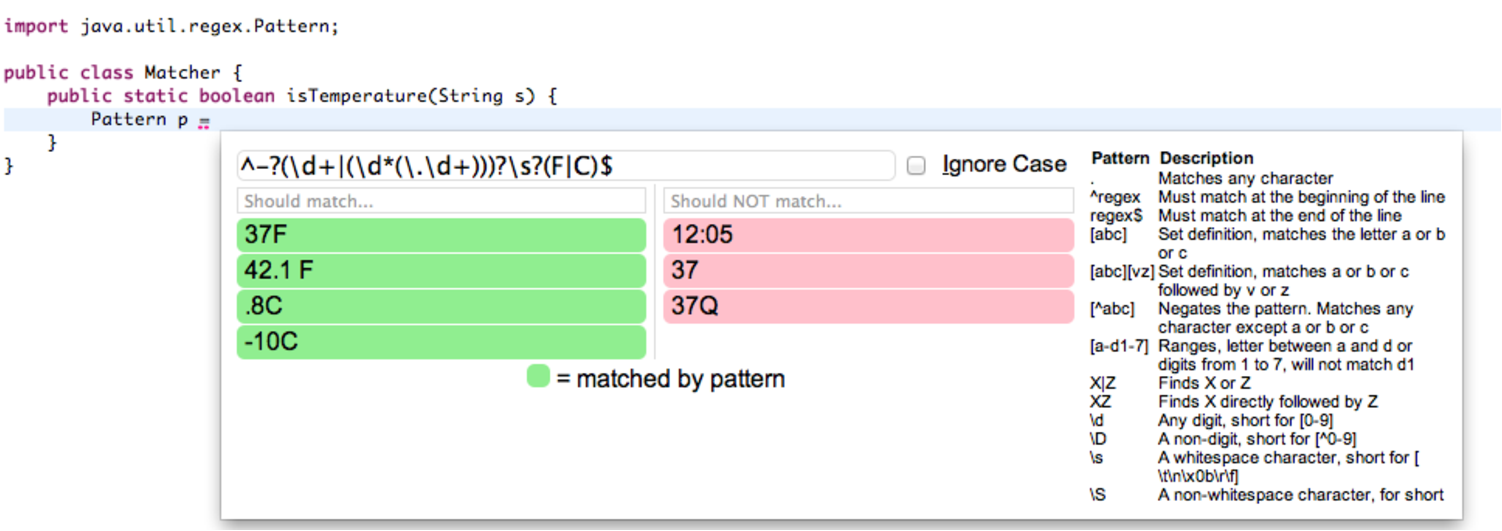
\includegraphics[scale=.55]{regex-palette.pdf}\\
% $\Downarrow$ \text{(pressing \textbf{Enter})}\\
% 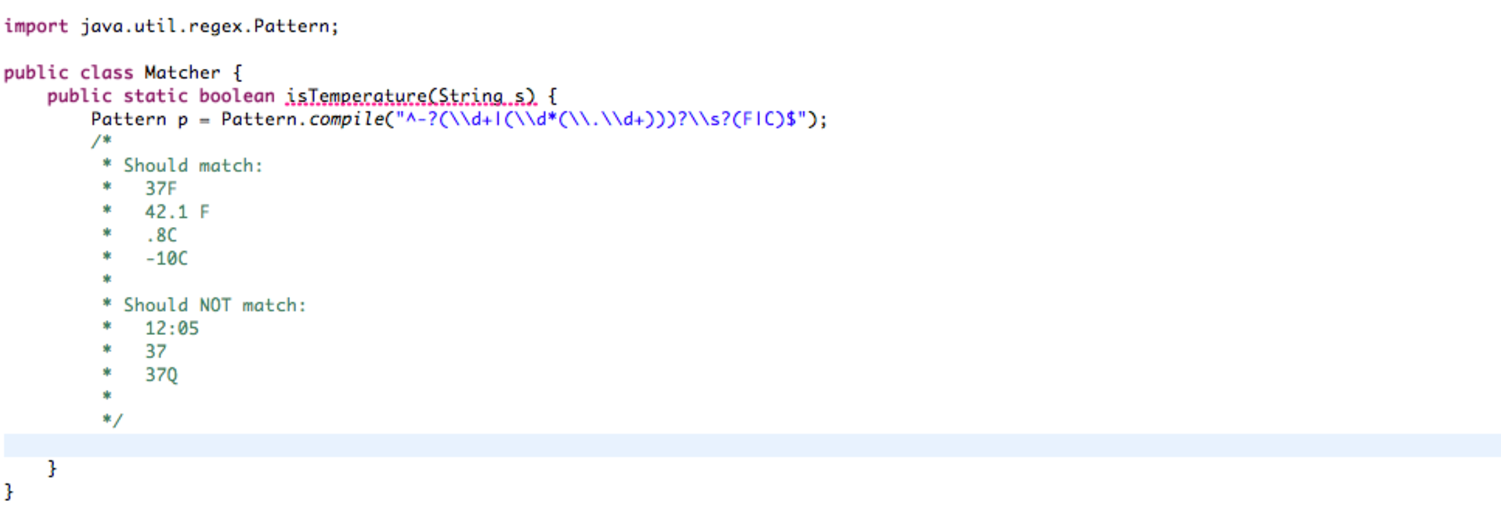
\includegraphics[scale=.55]{regex-code-generated.pdf}
% \end{center}
% \vspace{-20px}
% \caption{An example of type-specific editor services, here shown for Java.}
% \label{fig:regex-palette}
% %\vspace{-10px}
% \end{figure}

%In a conventional \emph{monolithic} programming system, support for each of these features would need to be built into the language and tools. 

\subsection{Existing Approaches}\label{sec:syntax-existing}
\subsubsection{Dynamic String Parsing}
To expose this more concise concrete syntax for regular expression patterns to clients, the most common approach is to provide a function that parses strings to produce patterns. Because, as just mentioned, there  may be many implementations of the \lstinline{PATTERN} signature, the usual approach is to define a parameterized module (a.k.a. a \emph{functor} in SML) defining utility functions like this abstractly:

\begin{lstlisting}[numbers=none]
module PatternUtil(P : PATTERN) => mod {
  fun parse(s : string) : P.t => (* ... pattern parser here ... *)
}
\end{lstlisting}
This allows a client of any module \lstinline{P : PATTERN} to use the following definitions:
\begin{lstlisting}[numbers=none]
let module PU = PatternUtil(P)
let val pattern = PU.parse
\end{lstlisting}
to construct patterns like this:
\begin{lstlisting}[numbers=none]
pattern "SSTRA|T|G|CESTR"
\end{lstlisting}
 %Again, none of our goals are comprehensively achieved.
Unfortunately, this approach is imperfect for several reasons:
\begin{enumerate} 
\item First, there are syntactic conflicts between string escape sequences and pattern escape sequences. For example, the following is not a well-formed term:
\begin{lstlisting}[numbers=none,mathescape=|]
let val ssn = pattern "SSTR\d\d\d-\d\d-\d\d\d\dESTR"
\end{lstlisting}
When compiling an expression like this, the client would see an error message like \verb|error: illegal escape character|.\footnote{This is the error message that \texttt{javac} produces. When compiling an analagous expression using SML of New Jersey (SML/NJ), we encounter the rather bizarre error message \texttt{Error: unclosed string}.} In a small lab study, we observed that this class of error was common, and often temporarily confused even experienced programmers if they had not used regular expressions recently \cite{Omar:2012:ACC:2337223.2337324}. The standard workaround has higher syntactic cost -- one must double all backslashes:
\begin{lstlisting}[numbers=none]
let val ssn = pattern "SSTR\\d\\d\\d-\\d\\d-\\d\\d\\d\\dESTR"
\end{lstlisting}

Some languages, anticipating such modes of use, build in alternative string forms that leave escape sequences uninterpreted. For example, Ocaml supports the following, which has only a constant syntactic cost:
\begin{lstlisting}[numbers=none]
let val ssn = pattern {rx|SSTR\d\d\d-\d\d-\d\d\d\dESTR|rx}
\end{lstlisting}

\item The next problem is that pattern parsing does not occur until the pattern is evaluated. For example, the following malformed pattern will only trigger an exception when this expression is evaluated during the full moon: %Achieving this goal is an explicit goal of this proposal, so we are obviously not happy with this.

\begin{lstlisting}[numbers=none]
case(moon_phase) {
    Full => pattern "SSTR(GCESTR" (* malformedness not statically detected *)
  | _ => (* ... *)
}
\end{lstlisting}
Though malformed patterns can sometimes be discovered dynamically via testing, empirical data gathered from large open source projects suggests that there remain many malformed regular expression patterns that are not detected by a project's test suite ``in the wild'' \cite{spishak2012type}. 

Statically verifying that pattern formation errors will not dynamically arise requires reasoning about the full dynamics of the language. This is an undecidable verification problem in general and is difficult to even partially automate. In this example, the verification procedure would first need to be able to establish that the variable \lstinline{pattern} is equal to the parse function \lstinline{PU.parse}. If the string argument had not been written canonically but rather computed, e.g. as \lstinline{"SSTR(GESTR" ^ "SSTRCESTR"} where \lstinline{^} is the string concatenation function applied in infix style, it would also need to be able to establish that this expression is equivalent to the string \lstinline{"SSTR(GCESTR"}. For patterns that are dynamically constructed based on input to a function (see example below), the problem is not solved by ``simply''  evaluating the expression statically (or, more generally, in some earlier ``stage'' of evaluation) \cite{Jones:Gomard:Sestoft:93:PartialEvaluation}. 

Of course, asking the client to provide a proof of well-formedness would completely defeat the purpose -- lowering syntactic cost.

\item Dynamic string parsing also necessarily incurs dynamic cost. Regular expression patterns are common when processing large datasets, so it is easy to inadvertently incur this cost repeatedly. For example, consider mapping over a list of strings:
\begin{lstlisting}[numbers=none]
map exmpl_list (fn s => rx_match (pattern "SSTRA|T|G|CESTR") s)
\end{lstlisting}
To avoid incurring the parsing cost for each element of \lstinline{exmpl_list}, the programmer or compiler must move the parsing step out of the closure or, barring that, ensure that an appropriately tuned memoization (i.e. caching) strategy is being used.\footnote{Anecdotally, in scientific code using major contemporary compilers, the former optimization is not automatic. Compilation caches are more often provided by the regular expression library, but like any cache, it is difficult to reason compositionally about performance in their presence.} %If the programmer does it, it can sometimes make the program more difficult to read. 

%This too is difficult if a portion of the pattern is dynamically generated. % Regular expressions are often used across large datasets in scientific applications, so the absolute peformance penalty can be non-trivial.

\item The next problem is that dynamic string parsing mainly decreases the syntactic cost of ``literal'' patterns. Patterns constructed compositionally cannot easily benefit from this technique. For example, consider this function from strings to patterns:
\begin{lstlisting}[numbers=none]
fun example(name : string) => 
  P.Seq(P.Str(name), P.Seq(pattern "SSTR: ESTR", ssn)) (* ssn as above *)
\end{lstlisting}
%We needed to use both dynamic string parsing and explicit applications of pattern constructors to achieve the intended semantics. 
It is difficult to capture idioms like this more concisely using dynamic string parsing (we will see an example of syntax that does capture such idioms below).

\item Finally, for functions like \lstinline{example} where we are constructing patterns on the basis of data of type \lstinline{string}, using strings coincidentally to introduce patterns makes it easy for programmers to use string concatenation in subtly incorrect ways. For example, consider the following seemingly more readable definition of \lstinline{example}:
\begin{lstlisting}[numbers=none,escapechar=|]
fun example_bad(name : string) => 
  pattern (name ^ "SSTR: \\d\\d\\d-\\d\\d-\\d\\d\\d\\dESTR")
\end{lstlisting}
%The (unstated) intent here was to treat \lstinline{name} as a sub-pattern matching only itself, but this is not the observed behavior when \lstinline{name} contains special characters that have other meanings in patterns.

Both \lstinline{example} and \lstinline{example_bad} have the same type and behave identically at many inputs, particularly those that would be expected during typical executions of the program (i.e. alphabetic names). It is only when the input \lstinline{name} contains special characters that have meaning in the concrete syntax of patterns that a problem arises. In applications that query sensitive data, mistakes like this lead to \emph{injection attacks}, which are among the most common and catastrophic security threats on the web today \cite{owasp2013}. Proving that mistakes like this have not been made involves reasoning about complex run-time data flows, so it is once again notoriously difficult to automate. 
 %Ultimately, of course, mistakes like this are the fault of a programmer using a flawed heuristic, and they could be avoided with discipline. The problem is once again that it is difficult to detect violations of this discipline automatically. 

 %Ideally, our library would be able to make it more difficult to inadvertently introduce subtle security bugs like this.
\end{enumerate}

% \begin{enumerate}
% \item \textbf{Conventional Concrete Syntax.} Patterns must be written in exactly the conventional manner, shown in blue below. Curly braces serve as an ``unquote'' form to splice one pattern into another:
% \begin{lstlisting}[numbers=none]
% let N : Pattern = /SURLA|T|G|CEURL/
% let BisI : Pattern = /SURLGC{EURLNSURL}GCEURL/
% let twoDigits : Pattern = /SURL\d\dEURL/\end{lstlisting}

% %The choice of delimiter, i.e. matching forward slashes here, is not important.
% %The cognitive load of reading and writing patterns is low and patterns are parsed once at compile-time. 
% \item \textbf{Compile-Time Parsing.} Pattern parsing must occur at compile-time, i.e. it must not incur run-time cost and malformed patterns, e.g. \lstinline{/SURLGC(EURL/}, must result in {compile-time} errors no matter where they appear in the program. 
% \item \textbf{Security By Default.} Strings must not be treated as patterns, nor used idiomatically to construct patterns. For example, the function below must be ill-typed because \lstinline{name} is not of type \lstinline{Pattern}:
% \begin{lstlisting}[numbers=none]
% fun example(name : string) : Pattern
%   let twoDigits : Pattern = /SURL\d\dEURL/
%   /SURL{EURLnameSURL}: {EURLtwoDigitsSURL}EURL/
% \end{lstlisting}
%     It is also acceptable for \lstinline{example("SSTR[a-z]ESTR")} to be equivalent to \lstinline{/SURL\[a-z\]: \d\d/}, i.e. strings are treated as patterns matching only themselves. 
% It is \emph{not} acceptable for \lstinline{example("SSTR[a-z]ESTR")} to be equivalent to \lstinline{/SURL[a-z]: \d\d/}. 

%     This is a security issue because if \lstinline{name} is derived from user input, such confusion could lead to \emph{injection attacks}, which are both common and catastrophic when using regular expression libraries that fail to achieve these goals, discussed below \cite{owasp2013}. 
%   %\item A more advanced semantics might ensure that out-of-bounds backreferences to a captured group do not occur \cite{spishak2012type}. For example, we would want \verb|BisI|, above, to have the more precise type \lstinline{Pattern(1)}, i.e. a pattern with one captured group. 
% % \end{enumerate}
% %When an error is found, an intelligible error message is provided.
% %\item An \textbf{implementation} that partially or fully compiles known regular expressions into the efficient internal representation that will be used by the regular expression matching engine (e.g., a finite automata \cite{Thompson:1968:PTR:363347.363387}) ahead of time. In most languages, this compilation step occurs at run-time, even if the pattern is fully known at compile-time, thereby introducing performance overhead into programs. If the developer is not careful to cache compiled representations, regular expressions used repeatedly in a program might be needlessly re-compiled on each use. %By performing this step ahead-of-time, these dangers can be avoided.
% %\item A range of \textbf{editor services} that support syntax highlighting for patterns, retrieval of relevant documentation, interactive testing, and pattern extraction from example strings have been shown to be helpful for programmers when working with complex regular expressions \cite{ACC_VLHCC}. An example of some of these is shown in Figure \ref{fig:regex-palette}: the editor service shown helps programmers generate correct code, here via the Java standard library's implementation of regular expressions (discussed below).
% \end{enumerate}
% Let us consider the ways that providers of regular expression libraries commonly choose to define the type \verb|Pattern|: as synonymous to \lstinline{string}, as a recursive sum type, or as an abstract type.

% \vspace{-5px}
% \paragraph{Patterns as Strings} The most na\"ive choice is to define \lstinline{Pattern} as synonymous to \lstinline{string}:

% \begin{lstlisting}[numbers=none]
% type Pattern = string
% \end{lstlisting}
% The only reason to consider this definition is that it allows us to approximate pattern syntax using standard string literal syntax:

% \begin{lstlisting}[numbers=none]
% let N : Pattern = "SSTRA|T|G|CESTR"
% \end{lstlisting}
% To splice one pattern into another, we can perform string concatenation:
% \begin{lstlisting}[numbers=none,escapechar=|]
% let BisI : Pattern = "SSTRGCESTR" ^ N ^ "SSTRGCESTR"
% \end{lstlisting}
% or use string interpolation (as in Scala or SML/NJ using quotation/antiquotation \cite{SML/Quote}):
% \begin{lstlisting}[numbers=none,mathescape=|]
% let BisI : Pattern = s"SSTRGC${ESTRNSSTR}GCESTR"
% \end{lstlisting}

% Though this comes close, goal 1 is not truly achieved because the syntax of strings can conflict with the syntax for patterns. 

% Goal 2 is not achieved because parsing occurs only at run-time when we match a string against a pattern (worse, every time we do so unless the implementation uses an effective caching strategy).

% Goal 3 is also not achieved because the following code typechecks:
% \begin{lstlisting}[numbers=none,mathescape=|]
% fun example_bad_1(name : string) : Pattern
%   let twoDigits : Pattern = "SSTR\\d\\dESTR"
%   s"SSTR${ESTRnameSSTR}-${ESTRtwoDigitsSSTR}"ESTR
% \end{lstlisting}
% but \lstinline{example_bad_1("SSTR[a-z]ESTR")} evaluates to \lstinline{"SSTR[a-z]-\\d\\dESTR"}.



% \paragraph{Patterns as Recursive Sums} A more semantically justifiable strategy is to define \lstinline{Pattern} as a recursive sum type  \cite{pfpl}. Verse supports these in the form of case types, which are analagous to datatypes in ML:

% \begin{lstlisting}[numbers=none]
% casetype Pattern
%   Empty
%   Str of string
%   Seq of Pattern * Pattern
%   Or of Pattern * Pattern
%   Star of Pattern  
% \end{lstlisting}

% More generally, we can hold the representation of patterns abstract while exposing an isomorphic interface to clients by defining an abstract type in a {module} opaquely ascribed the following {module type} (a.k.a. \emph{signature} in SML): % exposes the constructors and case analysis as functions:

% \begin{lstlisting}[deletekeywords={case},numbers=none]
% module type PATTERN
%   type t
%   val Empty : t
%   val Str : string -> t
%   val Seq : t * t -> t
%   val Or : t * t -> t
%   val Star : t -> t
%   val case : (
%     'a -> 
%     (string -> 'a) ->
%     (t * t -> 'a) ->
%     (t * t -> 'a) ->
%     (t -> 'a) ->
%     'a)
% \end{lstlisting}
% The client of any module \lstinline{P : PATTERN} can define \verb|Pattern| as synonymous to \verb|P.t|: 
% \begin{lstlisting}[numbers=none]
% type Pattern = P.t
% \end{lstlisting}



%The first one might not be found incorrect without rigorous testing with unexpected inputs. Goal 3 expresses the ideal of designing a language where security does not require considering such subtle issues extralinguistically.%This is precisely why injection attacks are so difficult to detect.

% The dialect of Standard ML implemented by SML/NJ, recognizing that directly using constructors is often less than ideal, provides a facility for quotation/antiquotation \cite{SML/Quote}, which if introduced into Verse could be used as follows:
% \begin{lstlisting}[numbers=none,escapechar=|,mathescape=|]
% fun example(p : string)
%   let twoDigits = P.qparse `SQT\d\dEQT`
%   P.qparse `SQT^(EQTP.Str(p)SQT)-^(EQTtwoDigitsSQT)EQT`
% \end{lstlisting}

% Here, backticks are used to indicate a quoted term within which carets serve as an antiquote operator. This still represents a  compromise against goal 1. The most serious problem is that, once again, parsing does not occur until run-time. There are also  conflicts between quotation syntax and pattern syntax, i.e. \verb|^| conventionally means character set negation inside patterns, which conflicts with antiquotation here. This mechanism also does not support antiquotation at more than one type, so we could not define the antiquote operator to insert the \verb|Str| constructor automatically, as suggested in goal 3. %For syntax that necessary involves antiquotation at multiple types (e.g. concrete syntax for a programming language with multiple syntactic sorts, HTML which might include Javascript and CSS, and others), this 

The problems above are not unique to regular expression patterns. Whenever a library encourages the use of dynamic string parsing to address the issue of syntactic cost (which is, fundamentally, not a dynamic issue), these problems arise. %Strings are, simply put, not ideally suited for this task. 
	This fact has motivated much research on reducing the need for dynamic string parsing \cite{Bravenboer:2007:PIA:1289971.1289975}. Existing alternatives can be broadly classified as being based on either \emph{direct syntax extension} or \emph{static term rewriting}. We describe these next, in Secs. \ref{sec:syntax-extension} and \ref{sec:term-rewriting} respectively.% We summarize the most relevant work below.

\subsubsection{Direct Syntax Extension}\label{sec:syntax-extension}
One tempting alternative to dynamic string parsing is to use a system that gives the users of a language the power to directly extend its concrete syntax with new derived forms. %for regular expression patterns.% for patterns.

The simplest such systems are those where the elaboration of each new syntactic form is defined by a single rewrite rule. For example, Gallina, the ``external language'' of the Coq proof assistant, supports such extensions \cite{Coq:manual}. A formal account of such a system has been developed by Griffin \cite{5134}. Unfortunately, these systems are not expressive enough to allow us to express pattern syntax in the conventional manner. For example, sequences of characters  can only be parsed as identifiers using these systems, rather than as characters in a regular expression pattern. 

Syntax extension systems based on context-free grammars like  Sugar* \cite{erdweg2013framework}, Camlp4 \cite{ocaml-manual} and several others, as well as mechanisms that allow direct programmatic control over parsing like Racket's reader extensions \cite{Flatt:2012:CLR:2063176.2063195} are more expressive, and would allow us to directly introduce pattern syntax into our core language's grammar, perhaps following Unix conventions like this:
\begin{lstlisting}[numbers=none]
let val ssn = /\d\d\d-\d\d-\d\d\d\d/
\end{lstlisting}

For patterns constructed compositionally, we can define \emph{splicing syntax} that allows us to write string and pattern expressions inline (distinguished by prefixes \lstinline{@} and \lstinline{%}, respectively). 
For example, we can write \lstinline{example} equivalently, but at lower syntactic cost, like this:
\begin{lstlisting}[numbers=none,escapechar=|]
fun example_concise(name : string) => 
  /@name: %ssn/
\end{lstlisting}
%The body of this function elaborates to the body of \lstinline{example_fixed} as shown above. 
Had we mistakenly written \lstinline{%name}, we would encounter only a static type error, rather than the  silent injection  vulnerability discussed above. 

The problems of dynamic string parsing described above are solved by this approach. Unfortunately, it introduces serious new problems. First, the systems mentioned thus far cannot guarantee that \emph{syntactic conflicts} between such extensions will not arise. As stated directly in the  Coq manual: ``mixing different symbolic notations in [the] same text may cause serious parsing ambiguity''. If another library provider used similar syntax for a different implementation or variant of regular expressions, or for some other unrelated construct, then a client could not simultaneously use both libraries at the same time. So properly considered, every combination of extensions introduced using these mechanisms creates a \emph{de facto} derived syntactic dialect of our language. % Resolving such parsing amibiguities is left to each client of the library. 

In response to this problem, Schwerdfeger and Van Wyk developed a modular analysis that accepts only grammar extensions that specify a universally unique starting token and obey subtle constraints on  the follow sets of base language non-terminals \cite{conf/pldi/SchwerdfegerW09}. Extensions that satisfy these criteria can be used together in any combination without the possibility of syntactic conflict. However, note that the most natural starting tokens like \lstinline{pattern} cannot be guaranteed to be universally unique, so we would be forced to use a more verbose token like \lstinline{edu_cmu_verse_rx_pattern}. There is no simple way for clients of our extension to define scoped abbreviations for starting tokens because this mechanism operates purely on syntactic forms.

Putting this aside, we must also consider the question of how newly introduced forms elaborate to forms in our base grammar. In our example, this is tricky because we have defined a modular encoding of patterns -- which particular module should the elaboration use? Clearly, simply assuming that some module identified as \lstinline{P} matching \lstinline{PATTERN} is in scope is a brittle solution. In fact, we should expect that the system actively prevents such capture of specific variable names to ensure that variables (including module variables) can be freely renamed. Such a \emph{hygiene discipline} is well-understood only when performing term-to-term rewriting (discussed below) or in simple language-integrated rewrite systems like those found in Coq. For mechanisms that operate strictly at the level of context-free grammars, this issue is not easy to address.

We can address the problem of choosing a module to use in the elaboration by requiring that the client explicitly identify it as an ``argument'' to the form:
\begin{lstlisting}[numbers=none]
let val ssn = edu_cmu_verse_rx_pattern P /\d\d\d-\d\d-\d\d\d\d/
\end{lstlisting}

Another problem with the approach of direct syntax extension is that there is no typing discipline -- given an unfamiliar piece of syntax, there is no straightforward method for determining what type it will have, causing difficulties for both humans (related to code comprehension) and tools. 

\subsubsection{Static Term Rewriting}\label{sec:term-rewriting}
An alternative approach is to leave the concrete syntax of the language fixed, but repurpose it for novel ends using a \emph{local term-rewriting system}. The LISP macro system \cite{Hart63a} is perhaps the most prominent example of such a system. Early variants of this system suffered from the problem of unhygienic variable capture just described, but  later variants, notably in the Scheme dialect of LISP, brought support for enforcing hygiene \cite{Kohlbecker86a}. In languages with a stronger static type discipline, variants of macros that restrict rewriting to a particular type and perform the rewriting statically have also been studied \cite{Herman10:Theory,ganz2001macros} and integrated into languages, e.g. MacroML \cite{ganz2001macros} and Scala \cite{ScalaMacros2013}. 

The most immediate problem with using these for our example is that we are not aware of any such statically-typed macro system that integrates cleanly with an ML-style module system, i.e. macros cannot be parameterized by modules. However, let us imagine such a macro system. We could use it to repurpose string syntax  as follows:
\begin{lstlisting}[numbers=none]
let val ssn = pattern P {rx|SSTR\d\d\d-\d\d-\d\d\d\dESTR|rx}
\end{lstlisting}

Here, \lstinline{pattern} is a macro parameterized by a module \lstinline{P : PATTERN}. It statically parses the provided string literal (which must still be written using an Ocaml-style literal here) to generate an elaboration. The macro specifies that the elaboration it statically generates will be of type \lstinline{P.t}. 
By parsing the string statically, we avoid the problems of dynamic string parsing for statically-known patterns. 

For patterns that are constructed compositionally, we need to get more creative. For example, we might repurpose the infix operators that are normally used for other purposes to support string and pattern splicing as follows:

\begin{lstlisting}[numbers=none,escapechar=|]
fun example_macro(name : string) => 
  pattern P (name ^ "SSTR: ESTR" + ssn)
\end{lstlisting}

Having to creatively repurpose existing syntax like this limits the impact a library provider can have on syntactic cost (particularly when there are pre-existing conventions that are not consistent with the conventions adopted by the language). It also can create confusion for readers expecting parenthesized expressions to behave in a consistent manner. However,  this approach is still common because it avoids many of the problems of na\"ive syntax extensions: there cannot be syntactic conflicts (because the syntax is not extended at all), we can define macro abbreviations because macros are integrated into the language, there is a hygiene discipline that guarantees that the elaboration will not capture variables inadvertently, and using a typed macro system, there is a clear type discipline (i.e. programmers need not examine the elaboration to know what type a macro application must have). 

% \begin{enumerate}
% \item Given an unfamiliar piece of syntax, there is no simple method for determining what type it has, or to identify which extension determines its desugaring, hindering code comprehension.
% \item It requires that the syntax be expressed as a grammar that can be consumed by a particular parser generator. Not all syntax  is most naturally expressed in this way, but there is no way to use a ``hand-rolled'' parser.
% \end{enumerate}

\subsection{Contributions}\label{sec:syntax-contributions}
Verse provides a new external primitive -- the \textbf{typed syntax macro} (TSM) -- that combines the syntactic flexibility of syntax extensions with the reasoning guarantees of typed macros. TSMs can be parameterized by modules, so they can be used to define syntax valid at any type defined by a module satisfying a specified signature. As we will discuss in Sec. \ref{sec:tsms} below, this addresses all of the problems brought up above, at moderate syntactic cost.

To further decrease syntactic cost (which is, of course, the entire purpose of this effort), we go on in Sec. \ref{sec:tsls} to briefly introduce \textbf{type-specific languages} (TSLs). TSLs are TSMs associated directly with a type when it is generated. Verse leverages local type inference to implicitly control TSL dispatch.

Syntax defined by library providers using these primitives comes at syntactic cost comparable to that of derived syntax built in primitively by the language designer or  using a na\"ive syntax extension tool like Camlp4, without causing dialect formation. As such, these \emph{ad hoc} approaches can, in large part, be discarded. That said, we examine some limitations of our approach in Sec. \ref{sec:tsms-limitations}.

\subsubsection{Typed Syntax Macros (TSMs)}\label{sec:tsms}
%A typed syntax macro is invoked by applying it to a \emph{delimited form}, which can contain  arbitrary syntax in its \emph{body}.  
To introduce TSMs, let us consider the following concrete external expression:
\begin{lstlisting}[numbers=none]
pattern P /SURLA|T|G|CEURL/
\end{lstlisting}
Here, we apply a \emph{parameterized TSM}, \lstinline{pattern}, first to a module parameter, \lstinline{P}, then to a \emph{delimited form}, \lstinline{/SURLA|T|G|CEURL/}. Note that a number of alternative delimiters are also provided by Verse's concrete syntax and could equivalently be used. The TSM statically parses the \emph{body} of the provided delimited form, i.e. the characters between the delimiters (shown here in blue), and computes an \emph{elaboration}, i.e. another external expression. In this case, \lstinline{pattern} generates the following elaboration (written concretely):

% import cs.cmu.edu/~wyvern/regex as R
% let syntax pattern = R.pattern
% let module P = R.P
% The first line imports our top-level regular expression module (identified uniquely by a URI) and binds a shorter name, \lstinline{R}, to it. The second line binds a local name to the  TSM named \lstinline{pattern} that \lstinline{R} exports. The third line gives a shorter name, \lstinline{P}, to the module \lstinline{R.P : R.PATTERN}, as defined previously. The fourth line then applies \lstinline{pattern} to this module parameter and a form delimited by forward slashes. This causes it to elaborate \emph{statically} to the following base form:
\begin{lstlisting}[numbers=none]
P.Or(P.Str "SSTRAESTR", P.Or(P.Str "SSTRTESTR", P.Or(P.Str "SSTRGESTR", P.Str "SSTRCESTR")))
\end{lstlisting}

%The original expression, above, is statically rewritten to this expression.
The definition of \lstinline{pattern} looks like this:
\begin{lstlisting}[numbers=none]
syntax pattern(P : PATTERN) at P.t {
  static fn (ps :: ParseStream) :: Exp => (* pattern parser here *)
}
\end{lstlisting}
This TSM definition first identifies the TSM as \lstinline{pattern}, then specifies a module parameter, \lstinline{P}, which must match the signature \lstinline{PATTERN}. Note that identifying the module parameter as \lstinline{P} here is an entirely local choice, i.e. the TSM can be applied to \emph{any} module parameter matching  \lstinline{PATTERN}. This parameter is used in the type annotation \lstinline{at P.t}, which specifies that all elaborations that arise from the application of this TSM to a module \lstinline{P} and a delimited form must necessarily be of type \lstinline{P.t}. These elaborations arise by the static action of the parse function defined next, within braces. It is written as a static function of sort \lstinline{ParseStream -> Exp}.  Both of these are defined in the Verse \emph{prelude}, which is a set of definitions available ambiently. The sort \lstinline{ParseStream} will give the function access to the {body} of the delimited form (in blue above) and the sort \lstinline{Exp}  encodes the abstract syntax of external expressions. %So the parse function parses the body of the delimited form to generate an encoding of the elaboration.

To support splicing syntax as described in Sec. \ref{sec:syntax-extension}, the parse function must be able to extract external subexpressions directly from the parse stream. For example, consider the client code below:
\begin{lstlisting}[numbers=none]
(* TSMs can be partially applied and abbreviated *)
let syntax pat = pattern P
let val ssn = pat /SURL\d\d\d-\d\d-\d\d\d\dEURL/
fun example_tsm(name: string) => 
  pat /SURL@EURLnameSURL: %EURLssn/
\end{lstlisting}
The subexpressions \lstinline{name} and \lstinline{ssn} on the last line occur directly in the parse stream. When the parse function encounters these, it asks the \lstinline{ParseStream} to extract these as \emph{spliced expressions} for use in the elaboration. For example, the elaboration generated for the body of \lstinline{example_tsm} above would, if written concretely with spliced expressions marked, be:
\begin{lstlisting}[numbers=none]
P.Seq(P.Str(<spliced>(name)), P.Seq(P.Str ": ", <spliced>(ssn)))
\end{lstlisting}
The hygiene mechanism then ensures that only these marked portions of the generated elaboration can refer to the variables at the use site, preventing inadvertent variable capture by the elaboration. For example, the following would not be a valid elaboration, because it has free variables that are not inside spliced subexpressions:
\begin{lstlisting}[numbers=none]
P.Seq(P.Str(name), P.Seq(P.Str ": ", ssn))
\end{lstlisting}
%Put another way, the  elaboration logic must be valid in any context. 

\paragraph{Formalization} To briefly introduce the formal specification of TSMs, let us consider the rule in the EL's semantics for handling TSM application to a delimited form. To simplify matters, we will first consider only unparameterized TSMs (i.e. TSMs defined at a single type, e.g. the case type \lstinline{Pattern}, rather than a parameterized family of types): 
\begin{mathpar}
\inferrule[syn-aptsm]{
    \vdash \psi ~@~ \sigma_\text{ty}~\{\sigma_\text{parser}\}\\
    \mathbf{parsestream}(b) = \sigma_\text{ps}\\
    \sigma_\text{parser}(\sigma_\text{ps}) \Downarrow \sigma_\text{elab}\\
    \sigma_\text{elab} \uparrow e_\text{elab}\\\\
    \Gamma; \emptyset \vdash e_\text{elab} \Leftarrow \sigma_\text{ty} \leadsto \iota_\text{trans}
}{
    \Gamma_\text{out}; \Gamma \vdash \mathbf{aptsm}(\psi; b) \Rightarrow \sigma_\text{ty} \leadsto \iota_\text{trans}
}
\end{mathpar}
Looking at the conclusion of the rule, we see that TSM application takes the abstract form $\mathbf{aptsm}(\psi; b)$. The metavariable $\psi$ ranges over \emph{TSM expressions} and $b$ ranges over {bodies} of delimited forms. TSM expressions consist only of TSM definitions here (cf. the definition of \lstinline{pattern} above), though when we formalize parameterized TSMs, we will distinguish TSM definitions from TSM expressions.%Note that for simplicity in the formal system, we have tacitly assumed that TSM names are drawn from a set that is disjoint from the set of variable names, so that function application and TSM application desugar to the distinct abstract forms. %In practice, we would use a common set of names and include a disambiguation step, but making the assumption of disjoint names allows us to avoid specifying this. %In practice, there would be an additional step that determined whether a function or a TSM was being applied based on the current context, 

Note also that we omit various contexts relevant only to other Verse primitives. We include only \emph{typing contexts}, $\Gamma$, which map variables to types in the standard way. We describe why there are two contexts -- the \emph{outer context} and the \emph{current context} -- below. 


The premises can be understood as follows, in order:
\begin{enumerate}
\item The first premise can be pronounced ``TSM expression $\psi$ defines a valid TSM at type $\sigma_\text{ty}$ with parse function $\sigma_\text{parser}$''.  The ``outputs'' of this judgement are the type $\sigma_\text{ty}$ (of sort $\mathsf{Ty}$) and the static parse function, $\sigma_\text{parser}$ (of sort $\mathsf{ParseStream} \rightarrow \mathsf{Exp}$), defined by the TSM.% We must omit the rules governing this judgement here (a complete specification of this judgement represents the main piece of remaining work, see below). % Application of a parameterized TSM to its parameters is handled by this judgement (not shown).
\item The second premise creates a parse stream, $\sigma_\text{ps}$, of sort $\mathsf{ParseStream}$, from the body of the delimited form.
\item The third premise applies the parse function to the parse stream to generate a static representation of the elaboration, $\sigma_\text{elab}$ (of sort $\mathsf{Exp}$).% Note that this is ``metaprogramming'' -- a static expression in the external semantics to generate an encoding of another external term.
\item The fourth premise decodes $\sigma_\text{elab}$, producing the elaboration itself, $e_\text{elab}$.
\item The final premise \emph{validates} the elaboration by analyzing it against the type $\sigma_\text{ty}$ specified by the TSM. The {current} typing context is ``saved'' for use when a spliced subexpression is encountered during this process by setting it as the new \emph{outer context}, as indicated.

Variables in the outer context are not directly available to the elaboration, e.g. they are ignored by the (syn-var) rule:
\begin{mathpar}
\inferrule[syn-var]{ }{
    \Gamma_\text{out}; \Gamma, x : \sigma \vdash x \Rightarrow \sigma \leadsto x
}
\end{mathpar}

Outer contexts are switched back in when encountering marked spliced expressions:
\begin{mathpar}
\inferrule[syn-spliced]{
    \emptyset; \Gamma_\text{out} \vdash e \Rightarrow \sigma \leadsto \iota
}{
    \Gamma_\text{out}; \Gamma \vdash \mathbf{spliced}(e) \Rightarrow \sigma \leadsto \iota
}

\inferrule[ana-spliced]{
    \emptyset; \Gamma_\text{out} \vdash e \Leftarrow \sigma \leadsto \iota
}{
    \Gamma_\text{out}; \Gamma \vdash \mathbf{spliced}(e) \Leftarrow \sigma \leadsto \iota
}
\end{mathpar}


This premise of (syn-aptsm) thus enforces both type safety and hygiene.

%The translation of the elaboration becomes the translation in the conclusion of the rule.
\end{enumerate}
%We plan to give a more complete account of all of these judgements in the dissertation.
\subsubsection{Type-Specific Languages (TSLs)}\label{sec:tsls}
With TSMs, we achieved the conventional syntax for regular expression patterns within delimiters, but we still explicitly had to apply the TSM and provide the module parameter each time. To further lower the syntactic cost of using TSMs, Verse also  supports \emph{type-specific languages} (TSLs). This allows library providers to associate a TSM directly with a generated type (or parameterized type constructor, more generally). For example, a module \lstinline{P} can associate \lstinline{pattern} with \lstinline{P.t} as follows:
\begin{lstlisting}[numbers=none]
module P : PATTERN = mod {
  type t = (* ... *)
  (* ... *)
} with syntax pattern
\end{lstlisting}

When the semantics encounters a delimited form not prefixed by a TSM name, the TSM associated with the type it is being analyzed against is implicitly applied. For example, the following function is equivalent to \lstinline{example_tsm} (note the return type annotation):
\begin{lstlisting}[numbers=none]
fun example_tsl(name : string) : P.t => 
  /SURL@EURLnameSURL: %EURLssn/
\end{lstlisting}

As another example, we can use TSLs to express derived list syntax. For example, if we use a case type, we can define the TSL directly upon declaring the list type:
\begin{lstlisting}[numbers=none]
casetype list('a) { Nil | Cons of 'a * list('a) } with syntax {
  static fn (body :: ParseStream) => 
    (* ... comma-delimited spliced exps ... *)
}
\end{lstlisting}
Together with the TSL for patterns, this allows us to write a list of patterns like this:
\begin{lstlisting}[numbers=none]
let val x : list(P.t) = [/SURL\dEURL/SHTML, EHTML/SURL\d\dEURL/SHTML, EHTML/SURL\d\d\dEURL/]
\end{lstlisting}
From the client's perspective, it is essentially as if the language had built in derived syntax for lists and regular expression patterns directly.%However, we did not need to build in this syntax primitively.%The only constraint is that this syntax must be used in an analytic position, which we argue is actually better for code compren when encountering unfamiliar syntax.

\subsubsection{Limitations}\label{sec:tsms-limitations}
%\todo{revise this section}The main limitation of this approach is that it 
Though elaboration validation ensures that an incorrect parser cannot threaten type safety,  proving type safety inductively is subtle because the elaboration is not a subexpression of the expression it will replace. There is a ``simple'' solution to this problem: we impose the restriction that the elaboration cannot itself use TSMs or TSLs. This would be somewhat awkward in practice, so we plan to briefly discuss other more flexible solutions as well.  

Another concern is that if we define the SL such that evaluating the parse function may not terminate, this then causes typechecking to become undecidable. In practice, this too should  be a minor concern. For example, we could specify a limit to the running time of the parse function. The compiler would enforce this limit to ensure that compilation does not ``hang'' due to an incorrect parser. Related concerns would arise if the static language supported external (e.g. I/O) effects. Existing techniques for controlling these effects would handle this problem, but this is not something we plan to detail here because our SL does not specify these effects.

Another limitation is that TSMs as we have described them only capture idioms that occur within a single parameterized family of types,  not idioms that might span many (or all) types, e.g. control flow idioms. In fact, this is intentional, as it makes maintaining a type discipline in the presence of TSMs substantially easier -- neither humans nor tools need to examine the elaboration to determine what type it must necessarily have. We will, however, discuss other points in the design space in the dissertation.

Finally, we have discussed only expression syntax here, but have not considered pattern matching. In fact, we conjecture that it is completely straightforward to extend this work to allow a TSM to define both an expression parser and a pattern parser. We plan to informally discuss this as the most immediate avenue for future work, but will not consider pattern matching in formal detail in the dissertation.

\subsection{Timeline and Milestones}\label{sec:syntax-timeline}
We described and gave a more detailed formal specification of TSMs in a recently published paper \cite{sac15}, and TSLs in a paper published last year \cite{TSLs}, both in the context of the Wyvern language. The mechanics of defining a TSM, statically invoking the parse function, elaboration encoding/decoding and hygienic elaboration validation have all been detailed there. In the dissertation, I plan to first present the formal system closely following this presentation, updating it only to ensure that it is consistent with the description above and with the work in the next section. The rule (syn-aptsm) above represents the first and most substantial step of this plan. I anticipate that this will take about \textbf{1.5 weeks} of further work.

Wyvern does not specify an ML-style module system (type declarations are the only form of type generation) and at the time, it did not support parameterized types, so to actually support the examples we have given in this section, we then need to update the formalization to handle parameterized TSMs. I plan to flesh this out in the course of writing the dissertation, and I anticipate it requiring 5.5 weeks of my time after the proposal is complete. I propose the following concrete milestones:

\begin{enumerate}
\item equip the EL with an appropriately structured module context \textbf{(2 weeks)}
\item formally specify the syntax of parameterized TSM expressions \textbf{(0.5 weeks)}
\item formally specify an updated version of the TSM expression validation judgement that appeared as the first premise of (syn-aptsm) above \textbf{(1 week)}
\item update the metatheory established in the work cited above to handle this \textbf{(2 weeks)}
\end{enumerate}

To validate our claims of expressiveness, I plan to give several more examples drawn from existing languages. I will include those we have worked out in the papers just cited as well as additional examples that highlight the benefits of integration with Verse's ML-based module system. For example, I will discuss implementing Haskell's primitive ``do'' syntax using TSLs together with a modular encoding of monads (as described on Prof. Harper's blog \cite{SML/Monads}). I will also show how parser generators and quasiquotation (e.g. as in Scala \cite{shabalin2013quasiquotes} or Lisp \cite{Bawd99a}) can be seen as modes of use of TSMs/TSLs. I will also briefly summarize the corpus analysis we conducted in \cite{TSLs} where we found a large number of  situations in large publicly available Java libraries where dynamic string parsing was apparently being used to control syntactic cost. I anticipate that writing these examples will take an additional \textbf{1 week} of work, bringing the total for this portion of the dissertation up to 8 weeks. %Adding in the time I will need to propose and some buffer time for unanticipated issues, my goal is to have this portion of the dissertation complete by the end of Summer 2015.



% \subsection{Typed Syntax Macros (and Type-Specific Languages)}
% Consider the following \emph{recursive case type}, which encodes the tree structure of HTML documents (we will see how case types are themselves library constructs later):
% \begin{lstlisting}[numbers=none]
% casetype HTML
%   Empty
%   Seq of HTML * HTML
%   TextNode of string
%   H1Element of Attributes * HTML (* Attributes not shown *)
%   (* ... *)
% \end{lstlisting}
% We can introduce values of this type by applying one of these declared constructors to data of the corresponding type. For example, here is a function that creates a heading given a string (assuming the variable \lstinline{empty_attrs : Attributes} is in scope, not shown):
% \begin{lstlisting}[numbers=none]
% fun make_heading(x : string) -> HTML
%   H1Element(empty_attrs, TextNode(x))
% \end{lstlisting}
% The same function can be written using more idiomatic HTML syntax via a TSM as follows:
% \begin{lstlisting}[numbers=none]
% fun make_heading_tsm(x : string)
%   html `SHTML<h1><%EHTMLxSHTML></h1>EHTML`
% \end{lstlisting}
% Here, \lstinline{html} identifies a TSM defined as below:
% \begin{lstlisting}[numbers=none]
% syntax html for HTML
%   fn (body : ParseStream) -> Exp => (* ... *)
% \end{lstlisting}
% The function in the indented block is invoked {statically} to generate an \emph{elaboration} based on the {body} of the \emph{delimited form} provided to the TSM, here \lstinline{SHTML<h1><%EHTMLxSHTML></h1>EHTML}, 
% for subsequent typechecking and translation to the Verse IL. In this example, the elaboration generated is equivalent to the one shown above in \lstinline{make_heading}. Both \lstinline{ParseStream}, which provides access to the body as a stream of characters, and \lstinline{Exp}, which encodes the abstract syntax of the Verse EL, are types defined in the Verse \emph{prelude}, which is simply a collection of definitions loaded before all others. The implementation of this parse function is not particularly interesting, so we omit it here. We will discuss how generating this function from a declarative grammar specification is itself a mode of use of TSMs later.

% Notice that a portion of the body, indicated in black for clarity, is treated as a \emph{spliced expression}. The TSM determines what syntactically distinguishes spliced expressions (here, the delimiters \lstinline{<%} and \lstinline{>} around an identifier or, not shown, \lstinline{<%>} and \lstinline{</%>} around an expression). 
% Verse only specifies the delimiters that can be used to transition from the expression language to the TSM body (here, we used backticks, but Verse supports several others, including \emph{layout delimiters}, which we will discuss later). This ensures that syntactic conflicts cannot arise by construction and localizes reasoning about syntactic ambiguity to each TSM, without incurring substantial syntactic cost.

% The semantics includes an \emph{elaboration validation} step that maintains a \emph{hygiene discipline} by ensuring that the elaboration does not make any assumptions about the context around the TSM application. In particular, only portions of the elaboration derived from spliced expressions can refer to variables in the surrounding context. Moreover, by requiring that the TSM provide a type annotation, it maintains a \emph{typing discipline}. For example, due to the type annotation on the definition of \lstinline{html} above, clients can assume that all successful applications of the TSM will elaborate to a term of type \lstinline{HTML}, without needing to reason about the elaboration logic itself. Not shown here, this annotation can be parameterized by types as well as modules. Because the Verse module system is borrowed directly from ML,  this means that TSMs can be used to define derived syntax valid for all instances of an abstract type. We will discuss this after motivating it with another example in Section \ref{sec:syntax}.

% To decrease the syntactic cost of applying a TSM even further (controlling syntactic cost being, of course, the very purpose of TSMs), Verse can often locally infer these parameters. Moreover, when a type is declared, Verse allows the library provider to designate one TSM as its \emph{type-specific language} (TSL). Clients can then omit mention of this TSM entirely in positions where an expression of that type is expected. For example, if \lstinline{html} was designated as the TSL for \lstinline{HTML}, then we could have written the function above equivalently as:
% \begin{lstlisting}[numbers=none]
% fun make_heading_tsl(x : string) -> HTML
%   'SHTML<h1><%EHTMLxSHTML%></h1>EHTML'
% \end{lstlisting}

%These mechanisms are one reason why we specify Verse by a bidirectionally typed elaboration semantics.

\section{Modularly Programmable Type Structure}\label{sec:metamodules}
In the previous section, we assumed that the EL had an otherwise standard, ML-like type structure and considered only TSMs and TSLs as departures from ML. In fact, constructs like case types (shown briefly in use in the previous section), tuples, records and objects are not built primitively into Verse. Instead, they can be expressed using \emph{metamodules} (which are distinct from, though closely related to, {modules}, as we will discuss below). Only polymorphic function types are built primitively into the Verse EL.

This section is organized like Sec. \ref{sec:syntax}. We will begin with examples of type structure that we might want to express in Sec. \ref{sec:metamodules-example}, then discuss how existing approaches are insufficient in Sec. \ref{sec:metamodules-related}. Next, we outline how {metamodules} (together with TSMs and TSLs) serve to address these problems in Sec. \ref{sec:metamodules-solution} and conclude with a timeline in Sec. \ref{sec:metamodules-timeline}.

\subsection{Motivating Example: Labeled Tuples and Regular Strings}\label{sec:metamodules-example}
As a simple introductory example, let us define a \emph{labeled tuple type} for conference papers:
\begin{lstlisting}[numbers=none]
let type Paper = ltuple {SPCT
   title : EPCTrstring /SURL.+EURL/
    SPCTconf : EPCTrstring /SURL([A-Z]+) (\d\d\d\d)EURL/
}
\end{lstlisting}
The \lstinline{let type} construction defines a synonym, \lstinline{Paper}, for a type constructed by applying the \emph{type constructor} (or \emph{tycon}) \lstinline{ltuple} to a \emph{component specification}, which is a  statically valued (cf. Sec. 2) ordered finite mapping from labels to types, written using conventional concrete syntax.

The first component is labeled \lstinline{title} and specifies the \emph{regular string type} \lstinline{rstring /SURL.+EURL/}. Regular string types are constructed by applying the tycon \lstinline{rstring} to a statically valued regular expression pattern, again written here using conventional concrete syntax like that discussed in the previous section. The second component of type \lstinline{Paper} is labeled \lstinline{conf} and specifies a regular string type with two {parenthesized groups}, corresponding to a conference abbreviation and year. 

% Alternatively, we could have used the following construction to declare \lstinline{Paper} \emph{generatively}:
% \begin{lstlisting}[numbers=none]
% lprodtype Paper {
%   SPCTtitle : EPCTrstring /SURL.+EURL/
%    SPCTconf : EPCTrstring /SURL([A-Z]+) (\d\d\d\d)EURL/
% }
% \end{lstlisting}
% The difference is in how type equality is handled. Two labeled product types with the same signature are equal, unless declared generatively, in which case type equality is nominal.

Clients can introduce regular strings in analytic position using standard string literal syntax, as long as the body of the literal is in the corresponding regular language. 
Clients can introduce a value of type \lstinline{Paper} in an analytic position in one of two ways. We can omit the labels and provide component values positionally:
\begin{lstlisting}[numbers=none]
let val exmpl : Paper = {"SUSAn Example PaperEUS"SCSS, ECSS"SUSEXMPL 2015EUS"}
\end{lstlisting}
Alternatively, we can include the component labels explicitly for readability or if we want to give the components in an alternative order:
\begin{lstlisting}[numbers=none]
let val exmpl : Paper = {SCSSconf=>ECSS"SUSEXMPL 2015EUS"SCSS, title=>ECSS"SUSAn Example PaperEUS"}
\end{lstlisting}
%In either case, notice that we used literal syntax to introduce the component values, which are of regular string type.

Given a value of type \lstinline{Paper}, we can project out a component value by providing  a  label:% like this:
\begin{lstlisting}[numbers=none]
let val exmpl_conf = # <SNATconfENAT> exmpl 
\end{lstlisting}
Here, \lstinline{#} identifies an \emph{operator constructor} (or \emph{opcon}) parameterized by a statically valued label, written literally here as \lstinline{<SNATconfENAT>}. The resulting \emph{operator}, \lstinline{# <SNATconfENAT>}, is then passed one \emph{argument}, \lstinline{exmpl}. An important point is that this operator is not a function, i.e. it cannot be given function type, because it is able to operate on values of \emph{any} labeled tuple type that has a component labeled \lstinline{conf}, not just \lstinline{Paper}. That type's component specification determines the type of the operation as a whole, here \lstinline{rstring /SURL([A-Z]+) (\d\d\d\d)EURL/}.

We can project out the first captured group from the regular string \lstinline{exmpl_conf} using the \lstinline{#group} operator constructor, which is parameterized by a statically valued natural number referring to the group index:
\begin{lstlisting}[numbers=none]
let val exmpl_conf_name = #group 0 exmpl_conf
\end{lstlisting}
The variable \lstinline{exmpl_conf_name} has type \lstinline{rstring /SURL[A-Z]+EURL/}.

We will equip labeled tuple types with an extended set of operators that go beyond the introduction and projection operators just discussed. For example, two labeled tuples can be concatenated (with common components updated with the value on the right) using the \lstinline{ltuple+} operator. Using this operator, we can add a component labeled \lstinline{authors} to \lstinline{exmpl}:
\begin{lstlisting}[numbers=none]
let val a : ltuple {SPCTauthors : EPCTlist(rstring /SURL.+EURL/)} = {["SUSHarry Q. BovikEUS"]}
let val exmpl_paper_final = ltuple+ exmpl a
\end{lstlisting}
We can drop a component using the operator constructor \lstinline{ltuple-}, which is parameterized by a static label:
\begin{lstlisting}[numbers=none]
let val exmpl_paper_anon = ltuple- <SNATauthorsENAT> exmpl_paper_final
\end{lstlisting}
There are many other operators that we might wish to describe, for both labeled tuples and regular strings, but for our purposes it suffices to stop here.

\subsection{Existing Approaches}\label{sec:metamodules-related}
Before describing how we express the type structure of labeled tuples and regular strings in Verse using metamodules, let us consider some alternative approaches for each.

\subsubsection{Labeled Tuples}
Recall that Verse builds only nullary and binary products into the IL, so we cannot express the type structure described above for labeled tuples  directly using IL primitives. The Verse EL does not build in even these, but so as to separate concerns, let us assume for the moment that regular string types are available in the EL: %So to consider existing approaches, we have to at least somewhat weaken our insistence on minimalism.
\begin{lstlisting}[numbers=none]
 (* type synonyms for concision *)
 let type title_t = rstring /SURL.+EURL/
 let type conf_t = rstring /SURL([A-Z]+) (\d\d\d\d)EURL/
\end{lstlisting}

\paragraph{Modules}
It is reasonable to ask if it is possible to express the type structure of any particular labeled tuple type using the module system.  %For simplicity below, let us slightly weaken our insistence on minimalism and build binary products into the EL (and, for now, assume that regular string types are also built in in some suitable manner).%This is not strictly necessary -- we could use a Church-style encoding -- but this simplifies our examples.%then we could try to use the module system to express the type structure of any particular labeled tuple type. For our example above:
For our example type \lstinline{Paper} from above, we might start by defining the following signature:
\begin{lstlisting}
signature PAPER = sig {
  type t
  (* introduction without labels *)
  val intro : title_t -> conf_t -> t
  (* introduction with explicit labels, in both orders *)
  val intro_title_conf : title_t -> conf_t -> t
  val intro_conf_title : conf_t -> title_t -> t
  (* projection *)
  val prj_title : t -> title_t
  val prj_conf : t -> conf_t
}
\end{lstlisting}
Here, we've taken all possible valid introductory and projection operators and called for their expression as functions. Expressing labels explicitly is an important facet of having labeled tuple types in a language, so we must put them into the function identifiers. Even with our minimal EL, we could  implement the semantics of the corresponding operators against this signature using a Church-style encoding (the details are standard and omitted here). Alternatively, if we slightly relax  our insistence on minimalism and add binary products to the EL, we could use them to implement our desired semantics like this:
\begin{lstlisting}
 module Paper : PAPER = mod {
   type t = title_t * conf_t
   fun intro title conf => (title, conf)
   fun intro_title_conf title conf => (title, conf)
   fun intro_conf_title conf title => (title, conf)
   fun prj_title (title, conf) => title 
   fun prj_conf (title, conf) => conf
 }
 \end{lstlisting}
%Compared to the four line type definition at the beginning of Sec.  safe to say that this is an  unacceptable departure from the four line type definition at the beginning of Sec. \ref{sec:metamodules-example}.

There are several fundamental problems with this approach. First, not every module matching the signature \lstinline{PAPER} correctly implements the semantics of the operators we seek to express, so each such module would itself need to be verified. In particular, we need to verify the universal condition that for all \lstinline{e : Paper.t} and \lstinline{f : Paper.t -> T}, we have that \lstinline{f(e)} is equivalent to \lstinline{f(Paper.intro (Paper.prj_title e) (Paper.prj_conf e))}. The volume of boilerplate code that needs to be generated and verified manually is factorial in the number of components of the labeled tuple type we are expressing (because we must encode each permutation of label orderings with a distinct introductory function).% Not all modules satisfying the signature above correctly implement the semantics, so this boilerplate must be checked for correctness in some way.

Even if we were to automate this (using, for example, \emph{type macros} as  in Scala \cite{ScalaMacros2013}, adapted to a language with ML-style modules), another issue is that we can only reasonably express the introductory and projection operators by specifying their semantics as functions like this. To enumerate all possible operators that arise from the opcon \lstinline{ltuple-} using functions would require constructing an encoding of every labeled tuple type that might arise from dropping one or more components from the labeled tuple in question. If fully enumerated, this would add an  exponential factor to our volume of boilerplate code. 
Finally, there is simply no way to specify the semantics \lstinline{ltuple+} with a finite collection of functions because there are infinitely many extensions of any labeled tuple type. % of this operator would need to be implemented by clients manually, defeating the purpose of the operator. %For example, there are an arbitrary 

% \begin{lstlisting}[numbers=none]
% signature PAPER
%   type t
%   val intro_tpl : rstring /.../ * rstring /.../ -> t
%   val intro_conf_title : rstring /.../ * rstring /.../ -> t
%   val intro_title_conf : rstring /.../ * rstring /.../ -> t
%   val prj_conf : t -> rstring /.../
%   val prj_title : t -> rstring /.../
%  \end{lstlisting}

\paragraph{Records and Tuples}
If, instead of this module-based encoding, we further weaken our insistence on minimalism and primitively build record and tuple types into the EL, as SML and many other languages have done, let us consider what might be possible. Note that these too are library constructs in Verse, but because they are so commonly built in to other languages, this situation is worth considering.%we can retreat from trying to use the module system, but have only slightly better options. 

The simplest approach we might consider taking is to directly map each labeled tuple type to a record type having an identically written component specification:
\begin{lstlisting}[numbers=none]
let type Paper_rcd = record {
  title : title_t
   conf : conf_t 
}\end{lstlisting}
Unlike labeled tuple types, record types are identified up to component reordering, so this mapping does not preserve certain type disequalities between labeled tuple types. Without positional information available in the type, it is not  possible to allow clients to omit component labels when introducing a value of record type.%, because this information is not maintained by the type system.

To work around this limitation if this is the only reason we care about preserving these type disequalities, we could define two conversion functions involving unlabeled tuples:
\begin{lstlisting}[numbers=none]
fun Paper_of_tpl (t : title_t, c : conf_t) => 
  {title => t, conf => c}
fun tpl_of_Paper {title => t, conf => c} =>
  (t, c)
\end{lstlisting}
For clients to be able to rely on this approach, we must extrinsically verify that the library provider implemented these functions correctly. Clients must also bear the syntactic and dynamic costs of explicitly invoking these functions. We could define a TSM for every such type to reduce this cost to clients, albeit at an additional cost to providers.  %This also means that we cannot omit the labels and rely on positional information when introducing a value of a record type in an analytic position, as we did above with type \lstinline{Paper}. %If we instead use an unlabeled product type (which in ML is actually a record type with numeric labels, which are omitted syntactically), we lose the ability to use labels in the elimination form. 

If, on the other hand, we do care about preserving all type disequalities between labeled tuple types, the workaround is even less elegant. We first need to define a record type with component labels tagged in some sufficiently unambiguous way by position, e.g.:
\begin{lstlisting}[numbers=none]
let type Paper = record {
	__0_title : title_t
	__1_conf : conf_t 
}\end{lstlisting}
To avoid exposing these labels directly to clients, we need two auxiliary type definitions:
\begin{lstlisting}[numbers=none]
let type Paper_tpl = (title_t * conf_t)
let type Paper_rcd = (* as above *)
\end{lstlisting}
and four conversion functions:
\begin{lstlisting}[numbers=none]
fun Paper_of_tpl (t : title_t, c : conf_t) => {
  __0_title => t,
  __1_conf => c
}
fun tpl_of_Paper {__0_title => t, __1_conf => c} => 
  (t, c)
fun Paper_of_rcd {title => t, conf => c} => {
  __0_title => t,
  __1_conf => c
}
fun rcd_of_Paper {__0_title => t, __1_conf => c} = {
  title => t,
  conf => c
}
\end{lstlisting}
Clients once again bear the costs of applying these conversion functions ahead of every operation and providers again bear the burden of defining this boilerplate code (which has volume linear in the number of components, albeit with a constant factor that is again not easy to dismiss) and verifying that these functions were implemented correctly. %We are interested in all such pragmatic issues, so this is not an entirely satisfying solution. % In any case, records, tuples and labeled tuples are all library constructs in Verse. 

As with the modular encoding of labeled tuples we attempted above, neither of these encodings using records and unlabeled tuples provides us with any way to uniformly express the more interesting operations, like \lstinline{ltuple+} or \lstinline{ltuple-}, that we discussed earlier.

\subsubsection{Regular Strings}
Let us now turn to regular string types. Note that we have specified the full semantics of regular string types in a recent workshop paper \cite{sanitation-psp14}.

\paragraph{Dynamic Checks}
The most common alternative to regular strings in existing languages is to simply use standard strings (which themselves may be expressed as lists or vectors of characters together with derived syntax) and insert dynamic checks around operations to maintain the regular string invariant. This clearly does not express the static semantics of regular strings, and incurs syntactic and dynamic cost.

\paragraph{Type Refinements}
We might attempt to recover the static semantics of regular strings by moving the logic governing regular string types into an external system of \emph{type refinements} \cite{Freeman91}. %This treats membership of a string in a specified regular language exclusively as a static verification condition. 
Such  systems allow programmers to specify \emph{refinements} of a type that capture more specific invariants. For example, we might consider capturing the regular string invariant using refinements of the \lstinline{string} type. Clients supply refinement specifications using structured comments or annotations (which can then be processed by external refinement checkers, like SML CIDRE \cite{Davies:1997:RTC}):
\begin{lstlisting}[numbers=none]
let val conf : string (* ~ rstring /([A-Z]+) (\d\d\d\d)/ *) = "EXMPL 2015"
\end{lstlisting}
One immediate limitation of this approach is that there is now no way to express the group projection operator described above, i.e. we cannot define a function \lstinline{#group} that can be applied like this:
\begin{lstlisting}[numbers=none]
let val conf_venue = #group 0 conf
\end{lstlisting}
The reason is that group projection does not have a function-like semantics -- it needs access to information that here is  available only in the type refinement of each regular string, i.e. the definitions of the captured groups. To access a group, we would instead need to dynamically match the string against the regular expression explicitly:

\begin{lstlisting}[numbers=none]
let val conf_venue = nth 0 (match /SURL([A-Z]+) (\d\d\d\d)EURL/ conf)
\end{lstlisting}
This has higher syntactic and dynamic cost. Moreover, proving that there will not be an out-of-bounds error in expressions like this requires more sophisticated reasoning about dynamic behavior.
%Refinement types are strictly a layer above the language, and thus cannot affect its dynamic semantics.

Another consideration is that type refinements do not introduce type disequalities. As a result, a compiler cannot use the invariants they capture to optimize the representation of a value. For example, the fact that some value of type \lstinline{string} can be given the refinement \lstinline{rstring /A|B/} cannot be justification to locally alter its representation to, for example, a single bit, both because it could later be passed into a function expecting a standard string and because there are many other possible refinements. Another perhaps more useful optimization that is not possible is to represent regular strings that have captured groups in a manner that ensures that group projection has constant dynamic cost (by running the match once when the string is introduced and caching the group values). Another example where this is relevant is when a language designer considers omitting a primitive type of ``non-negative integers representable in 32 bits'' because this seems ``merely'' to be a refinement of (mathematical) integers. But by eliminating the structural distinction between the two types, compilers lose the ability to use a machine representation more suitable to this particular static invariant. Of course, such structural distinctions  are sometimes inconvenient because they require defining and applying coercions with possibly non-zero dynamic cost to go from values of one type to another. Nevertheless, it is certainly not the case that a language can reasonably predict all possible structural distinctions that might be useful \emph{a priori}.

%Put another way, type refinements are quite useful when one needs only to make ``behavioral'' distinctions within a type, but they are not appropriate when new type disequalities would be useful or new operators need to be introduced.   %Refinement types cannot be used for this purpose without the possibility of conflict.
%This is also the reason why one cannot viably do away with primitive record types by claiming that they are refinements of finite mappings with labels as keys.

%In summary, type refinements are appropriate when one needs only to make finer static distinctions within an existing type. When one needs to introduce new operators or type disequalities that have ``downstream'' impact, refinement types are not the right solution.%Refinement types are useful when no non-trivial operators need to be introduced into the language and the refinement has no impact on representation, but the type system itself must be extended in some way in more advanced situations.


% \paragraph{Modules}
% To create type disequalities, we might consider again turning to the module system, defining a signature for each regular string type that we wish to work with. Again, this requires a non-trivial amount of boilerplate code:
% \begin{lstlisting}[numbers=none]
% signature TITLE = sig {
%   type t
%   val intro : string -> t
%   val strcase : t -> (unit -> 'a) -> (string * string -> 'a) -> 'a
% }

% signature CONF_GROUP_1 = sig {
% 	type t
% 	val intro : string -> t
% 	val strcase : t -> (unit -> 'a) -> (sting * strng -> 'a) -> 'a 
% }

% signature CONF = sig {
%   type t
%   val intro : string -> t
%   val strcase : t -> (unit -> 'a) -> (string * string -> 'a) -> 'a
%   structure Grp0 : CONF_GROUP_0
%   structure Grp1 : CONF_GROUP_1
%   val prj_group_0 : t -> Grp0.t
%   val prj_group_1 : t -> Grp1.t
% }

% \end{lstlisting}

% As discussed previously, we do not have a guarantee that all implementations of these signatures correctly capture the semantics we seek to express, so they must each be verified externally. Moreover, we must externally verify that every application  of the \lstinline{intro} operator is statically correct as well (i.e. that it won't raise an exception), perhaps with a system of type refinements. As with all language-external verification approaches, it is difficult to propagate this fact into a compiler in a manner that guarantees that redundant dynamic checks are eliminated. And finally, this approach again reveals itself to be too limited when we need to express operators that cannot be expressed as functions. For example, expressing regular string concatenation uniformly using a single function or a finite set of functions is impossible, because there are infinitely many regular string types that might be involved.

\subsection{Contributions}\label{sec:metamodules-solution}

%An important point is that labeled products, as well as other ``record-like'' constructs, can  be expressed by a \emph{type-directed translation} targeting our IL (and indeed, many compilers take advantage of facts like this to simplify the number of cases that must be considered downstream). %it is inaccurate to state that they are merely syntactic sugar over such a language. %Object systems are perhaps even more diverse across languages\todo{citation}. 
%Other dialects are justified by a desire to proivde more special-purpose semantic constructs. For example, 
%Substantially more sophisticated examples require at most only a very slightly more capable intermediate language (the IL of popular virtual machines, even those with flaws like ubiquitous \texttt{null} references, e.g. JVM or CIL bytecode, are also sufficient if used strictly as translation targets).

Verse introduces a \emph{metamodule system} that gives library providers more direct control over the type structure of the EL. Using the metamodule system, library providers can express all of the types and operators discussed above.

Just as the Verse (i.e. ML) module system is organized around \emph{signatures} and \emph{modules}, the Verse metamodule system is organized around \emph{metasignatures} and \emph{metamodules}. These are most easily introduced by example. We consider only labeled tuple types in this section (regular string types will follow analagously; we will discuss regular string types in more detail in the dissertation).
%Briefly summarized:
%\begin{itemize}
%\item A \emph{metasignature} specifies a set of type and operator constructors (tycons and opcons). Each is parameterized by a specified \emph{kind} of \emph{static value}. 
%\item A \emph{metamodule}  defines static functions that govern the typechecking and  translation to the IL of each type and operator constructor specified in the  metasignature. 
%\end{itemize}

%Static values are values of the \emph{typed static language} (SL), which itself forms a total typed lambda calculus, with \emph{static expressions} $\sigma$ classified by \emph{kinds} $\kappa$. Types are one kind of static value. We discuss other kinds of static values below.

\subsubsection{Example: Labeled Tuple Types via Metamodules}

Figure \ref{fig:ltuplex} defines a metasignature, \lstinline{LTUPLE}, and a matching 
metamodule, \lstinline{Ltuple}. It also defines a \emph{metamodule-parameterized TSM} \lstinline{ltpl}, which will give us the introductory syntax shown in Sec. \ref{sec:metamodules-example}. The remainder of this subsection explains this figure.

\paragraph{Type Constructors} On line \ref{line:ltuplex-c-sig} of Figure \ref{fig:ltuplex}, the metasignature \lstinline{LTUPLE} specifies that all matching metamodules must define a type constructor \lstinline{c} parameterized by {static values} of {sort} \lstinline{ComponentSpec}. %This user-defined sort (not shown) classifies ordered mappings from labels (of sort \lstinline{Lbl}, also user-defined but not shown) to types, which are static values of sort \lstinline{Ty} (a primitive sort). 
Let us assume that we can write static values of sort \lstinline{ComponentSpec} concretely like this (in the dissertation, we will discuss how it would be possible to adapt TSLs to also operate at the level of static values):
\begin{lstlisting}[numbers=none]
let static val Paper_tyidx :: ComponentSpec = {
  SPCTtitle : EPCTrstring /SURL.+EURL/SPCT,EPCT
   SPCTconf : EPCTrstring /SURL([A-Z]+) (\d\d\d\d)EURL/
}
\end{lstlisting}
Applying the type constructor \lstinline{Ltuple.c} to this parameter gives us a type:
\begin{lstlisting}[numbers=none]
let type Paper = Ltuple.c Paper_tyidx
\end{lstlisting}
Line \ref{line:tycon-synonym} defines the tycon synonym \lstinline{ltuple} for \lstinline{Ltuple.c}. Substituting into the above, we recover the definition of \lstinline{Paper} given at the beginning of Sec. \ref{sec:metamodules-example}:
\begin{lstlisting}[numbers=none]
let type Paper = ltuple {
  SPCTtitle : EPCTrstring /SURL.+EURL/SPCT,
   conf : EPCTrstring /SURL([A-Z]+) (\d\d\d\d)EURL/
}
\end{lstlisting}
Note that because types are static values of sort \lstinline{Ty}, this is equivalent to writing:
\begin{lstlisting}[numbers=none]
let static val Paper :: Ty = ltuple {
  SPCTtitle : EPCTrstring /SURL.+EURL/SPCT,
   conf : EPCTrstring /SURL([A-Z]+) (\d\d\d\d)EURL/
}
\end{lstlisting}

Also note that to ensure that type equality is decidable, tycon parameters can only be of a sort for which equality coincides with structural comparison of values. We call these sorts \emph{equality sorts}. Equality sorts are exactly analagous to equality types as found in Standard ML. The main implication of this restriction is that type parameters cannot contain static functions (because they cannot be compared structurally).

\paragraph{Type Translations} Recall from Sec. \ref{sec:verse} that each external type must translate to an internal type. Each metamodule controls the translation of types constructed by its tycons by defining a static function called the \emph{type translator}. This static function programmatically generates the type's translation given its type parameter. Type translations are represented as static values of sort \lstinline{ITy}, which we assume supports standard \emph{quasiquotation} syntax (e.g. as in Scala \cite{shabalin2013quasiquotes} or Lisp \cite{Bawd99a}).

The  type translator for \lstinline{Ltuple.c} is defined on lines \ref{line:c-start}-\ref{line:c-end} of Figure \ref{fig:ltuplex}. We have chosen here to translate labeled tuple types to nested binary product types internally. The type translator generates these by folding over the component mapping (using helper function \lstinline{comp_spec_to_tuples :: ComponentSpec -> list(Lbl * Ty)}, not shown). It generates the representation of \lstinline{unit} for the empty case, and nests the binary product types in the recursive case (using the standard \emph{unquote} syntax, \lstinline{%}). 
For example, the representation of the type translation of \lstinline{Paper} determined by this static function is:
\begin{lstlisting}[numbers=none]
`SCSStrans(ECSSrstring /SURL.+EURL/SCSS) * (trans(ECSSrstring /SURL([A-Z]+) (\d\d\d\d)EURL/SCSS) * unit)ECSS`
\end{lstlisting}
Notice that the translations of the component regular string types are not inserted directly, but are rather treated {parametrically} using the \emph{translational form} \lstinline{SCSStrans(ECSSTSCSS)}. This will be key to the modularity principle -- \emph{translation independence} -- that we will discuss shortly.%\todo{discuss SL}

Let us assume, for example, that all regular string types translate to standard internal strings, encoded by some internal type abbreviated \lstinline{string}. After we substitute this in for these translational forms, we arrive at the translation of \lstinline{Paper}:
\begin{lstlisting}[numbers=none]
string * (string * unit)
\end{lstlisting}

Formally, we should be able to derive that $\vdash \texttt{Paper}~\mathtt{type} \leadsto \texttt{string} \times (\texttt{string} \times \mathsf{unit})$. The following rule governs type translation:
\begin{mathpar}
\inferrule[trans-ty]{
    \vdash_\Phi \mathbf{ty}(m\cdot c; \sigma_\text{param}) :: \mathsf{Ty}\\
    \mathbf{ty}(m\cdot c; \sigma_\text{param})~\mathtt{sval}_\Phi\\
	\mathbf{translator}(\Phi; m\cdot c)=\sigma_\text{translator}\\
	\sigma_\text{translator}(\sigma_\text{param}) \Downarrow \sigma_\text{trans}\\
	\sigma_\text{trans} \uparrow_\Phi^m \tau_\text{abstrans} \parallel {\delta} : {\Delta}\\
	{\Delta} \vdash \tau_\text{abstrans}~\mathtt{itype}
}{
	\vdash_\Phi \mathbf{ty}(m.c;\sigma_\text{param})~\mathtt{type}\leadsto[{\delta}]\tau_\text{abstrans}
}
\end{mathpar}
Note that this rule is again slightly simplified here. It would need to be modified to handle external type abstraction, for example. However, it is pedagogically useful to begin with this simpler rule. Note that our purpose in this proposal is not to give a complete formal account of our contributions, but only to sketch out what this formal account will look like. 

Looking at the conclusion of the rule, we see that in the abstract syntax of the SL, types constructed by user-defined tycons take the form $\textbf{ty}(m\cdot c; \sigma_\text{param})$, where $m\cdot c$ refers to a  {tycon} $c$ defined by metamodule $m$ and $\sigma_\text{param}$ is the type parameter. The premises can be understood as follows:
\begin{enumerate}
\item The first premise checks that the type is of the required sort, $\mathsf{Ty}$. This involves finding the parameter sort associated with the tycon in the \emph{metamodule context}, $\Phi$ (we omit the straightforward definitions and rules for concision here).
\item The second premise checks that the parameter is a static value. %All static expressions, including types, are fully evaluated during typechecking and translation.
\item The third premise looks up the translator associated with $m \cdot c$ in $\Phi$. 
\item The fourth premise applies this translator to the type parameter to generate the representation of the type translation, $\sigma_\text{trans}$ (e.g. shown above for \lstinline{Paper}).
\item The fifth premise decodes $\sigma_\text{trans}$ to produce an \emph{abstracted type translation}, $\tau_\text{abstrans}$. It is ``abstracted'' in that translational forms referring to types constructed by metamodules other than $m$, e.g. \lstinline{trans(rstring /.+/)} above, have been replaced by type variables. For example, the representation above produces the abstracted typed translation $\alpha_1 \times (\alpha_2 \times \mathsf{unit})$. The actual translations of these types are packaged into a standard \emph{type substitution}, $\delta$. For example, here $\delta = [\texttt{string}/\alpha_1, \texttt{string}/\alpha_2]$. The context corresponding to this substitution, here $\Delta=\alpha_1, \alpha_2$, is also generated.
\item The final premise validates the abstracted type translation under $\Delta$ by making sure it is a valid internal type according to the internal statics.
\item Finally, the conclusion of the rule applies $\delta$ to the abstracted translation to produce the final type translation.
\end{enumerate}

We will see why having this ability to selectively hold type translations abstract is critical to modularity after we consider operator constructors.

\paragraph{Operator Constructors} On line \ref{line:intro-unlabeled-sig} of Figure \ref{fig:ltuplex}, the metasignature \lstinline{LTUPLE} specifies an operator constructor, \lstinline{intro_unlabeled}, parameterized by static values of sort \lstinline{unit}. The qualifier \lstinline{ana} specifies that this opcon is only for use in analytic positions (i.e. where the expected type is known). For example, we can apply \lstinline{Ltuple.intro_unlabeled} as follows, because the return type of the function determines the expected type:
\begin{lstlisting}[numbers=none]
fun make_paper(c : conf_t, t : title_t) : Paper => 
  Ltuple.intro_unlabeled () (c; t)
\end{lstlisting}
First, we provided the opcon with a static parameter value of the appropriate sort, here \lstinline{unit}, to create an operator. Then, we supply the operator with an \emph{argument list}, \lstinline{(conf; title)}.

This is syntactically unwieldy. Luckily, we can define a parameterized TSM, \lstinline{ltpl}, that gives us a more conventional syntax. As shown on lines \ref{line:ltplx-tsm-start}-\ref{ltplx-tsm-end} of Figure \ref{fig:ltuplex}, \lstinline{ltpl} defines syntax at all types that are of the form \lstinline{L.c(param)}, where \lstinline{L} is a metamodule matching \lstinline{LTUPLE} and \lstinline{param} is a static value of sort \lstinline{ComponentSpec}. In other words, the TSM defines syntax for all labeled tuple types. We elide the parser implementation, but as the comment indicates, we can rewrite \lstinline{make_paper} like this:
\begin{lstlisting}[numbers=none]
fun make_paper_tsm(c : conf_t, t : title_t) : Paper => 
  ltpl Ltuple Paper_tyidx {cSCSS, ECSSt}
\end{lstlisting}

To avoid having to explicitly name the TSM and supply the parameters, we designate \lstinline{ltpl} as \lstinline{Ltuple.c}'s TSL on line \ref{line:ltplx-annotation}. Now we can rewrite \lstinline{make_paper} in the standard way:
\begin{lstlisting}[numbers=none]
fun make_paper_tsl(c : conf_t, t : title_t) : Paper => 
  {cSCSS, ECSSt}
\end{lstlisting}

Putting syntax aside, the metamodule defining the opcon, \lstinline{Ltuple}, programmatically determines how to typecheck and translate this operation, again by the defining a static function called the \emph{opcon definition}. The definition of \lstinline{intro_unlabeled} is shown on lines \ref{line:introul-start}-\ref{line:introul-end} of Figure \ref{fig:ltuplex}. For analytic opcons like \lstinline{intro_unlabeled}, the semantics provides the opcon definition  with the type that the expression is being analyzed against, here \lstinline{Paper}, the operator parameter, here \lstinline{()}, and a list of \emph{argument interfaces}, which will allow it to ask the semantics to recursively typecheck and translate the arguments provided in the argument list. It must return a representation of an  internal expression, which will become the translation of the operation. Internal expressions are represented as static values of sort \lstinline{IExp}, and again we assume that we can use standard quasiquote syntax. The remaining opcons (which we will not consider in detail here) are synthetic opcons, which means they can be used anywhere. Rather than taking a type as input, they produce a pair of a type and a translation as output. 

On lines \ref{line:introul-start}-\ref{line:introul-end}, the opcon definition first checks that the type is actually a labeled tuple type using the \lstinline{tycase} primitive, which case analyzes against the type constructor of the provided type. There must always be a default case to ensure exhaustiveness. In this example, the default case raises a type error (with an error message, elided here).\footnote{The reason why we use this exception-like data flow for raising type errors, rather than using an option sort, is somewhat subtle so we defer it for discussion in the dissertation.} If the tycon is \lstinline{c}, we pair up the items in the type's component specification with the arguments and fold over this list. The empty case generates the representation of the trivial internal value and the recursive case generates nested pairs. Notice that this follows the structure of the type translator for \lstinline{c}, reflecting the fact that introductory operations at a type must generate a translation consistent with the corresponding type translation for type safety to hold. The static operation \lstinline{ana(arg, ty)} requests that the provided argument be analyzed against the provided type, evaluating to a representation of its translation if this succeeds and raising an error if it fails. For our example above, the representation of the translation generated by the opcon definition is:
\begin{lstlisting}[numbers=none]
`SQT(anatrans[0](EQTconf_tSQT), (anatrans[1](EQTtitle_tSQT), ()))`
\end{lstlisting}
An \emph{argument translation} of the form \lstinline{SQTanatrans[i](EQTTSQT)} stands in for the translation of argument \lstinline{i} analyzed against type \lstinline{T}.

The semantics next generates an \emph{abstracted translation}, which is a corresponding internal term where each argument translation has been replaced by a corresponding fresh variable. To validate it, we assume that the type of each variable is the abstracted type translation of the type the corresponding argument was analyzed against. So in this case, the abstracted translation is $(x_0, (x_1, ()))$ and it will be validated against the abstracted type translation for \lstinline{Paper}, i.e. $\alpha_0 \times (\alpha_1 \times \mathsf{unit})$, under a context where $x_0 : \alpha_0$ and  $x_1 : \alpha_1$ (this will, of course, succeed). Only after this succeeds are the actual argument translations substituted in to generate the final operation translation, here $({c}, ({t}, ())$.

By treating the arguments to the operation parametrically in this way, we can be sure that the metamodule defining labeled tuple types cannot violate the translation invariants that other metamodules maintain. For example, even if regular strings are implemented (by some other metamodule, not shown) as strings satisfying the regular string invariant, \lstinline{Ltuple} knows only that \emph{there exists} some translation for each regular string type, but nothing more. Thus, it cannot define ``bad'' opcons like this:

\begin{lstlisting}[numbers=none]
syn opcon bad {
	static fn (op_param :: unit, args :: list(Arg)) :: Ty * IExp => 
	  (rstring /.+/, `""`)
}
\end{lstlisting}
Here, the opcon ignores the arguments and synthesizes a regular string type that the client will assume classifies non-empty strings. However the corresponding translation is in fact the empty string. So even if all of the opcons defined in the metamodule implementing regular strings maintained this regular string invariant, this opcon would violate it. Note  that simply checking the translation is  well-typed would not solve this problem. The operator translation (the empty string) is consistent with the type translation (\lstinline{string}). Fortunately, by holding the type translation of regular strings abstract when validating the output of this opcon, the problem is caught -- the empty string is not of type $\alpha$. Put another way, the problem with this opcon is that it is not defined in a translation-independent manner with respect to tycons defined in another metamodule. This is exactly analagous to the representation independence property underlying modular reasoning with ML-style modules. By leveraging type abstraction, we are able to achieve modularity guarantees without requiring mechanized proofs of translation invariants (just as ML does not require mechanized proofs of representation invariants). 

%If the regular string metamodule later decides to change how it implements regular string types, this would require only local changes to that metamodule. We call this property \emph{translation independence}, by analogy to the \emph{representation independence} property that underlies modular reasoning with ML modules. %Translation independence allows library providers to reason locally about \emph{translation invariants} maintained by the operators in a metamodule. For example, a metamodule defining regular string types would maintain the regular string invariant. No other metamodule, by virtue of this translation independence property, can violate this invariant.

To formalize the intuition just described, we will need to introduce a non-trivial number of technical devices. It would thus require too much space to give a comprehensive formal account of this mechanism in this proposal, so  we leave this as work that remains to be done (though see below for progress). In broad strokes, it is similar to the rule for type translation described above in that we validate the operation translation before applying the substitutions for type and expression variables.

Note that the static functions that define these opcons contain code that looks just like the code that would appear in a standard implementation of the first stage of a compiler for a language that built in labeled tuple types. The novelty is not in these definitions, but in how they are organized and brought into the language.
% \begin{mathpar}
% \inferrule[ap-anaop]{
%   \mathbf{ana opcon}~m.\text{op}~\mathbf{of}~\uppi_\text{param}~\{ \sigma_\text{opdef} \} \in \Phi\\
%   \vdash_\Phi \sigma_\text{param} :: \uppi_\text{param}\\
%   \mathbf{args}(\es) = \sigma_\text{args}\\
%   \sigma_\text{opdef} (\sigma_\text{ty}) (\sigma_\text{param}) (\sigma_\text{args}) \Downarrow_{\hat{\Gamma};\Phi;\es} \sigma_\text{trans}\\
%   \sigma_\text{trans} \parallel \emptyset~\emptyset \uparrow_{\hat{\Gamma}; \Phi; \es}^m \tau_\text{abstrans} \parallel \memD~\memG\\
%   \mathsf{trans}(\sigma_\text{ty}) \parallel \memD \uparrow_{\Phi}^m 
% }{
% 	\hat{\Gamma} \vdash_\Phi \mathbf{opconap}(m; \text{op}; \sigma_\text{param}; \bar{e}) \Leftarrow \sigma_\text{ty} \leadsto [\delta][\gamma]\iota
% }
% \end{mathpar}
% omega anaop of pi_param { sigma_opdef }
% sigma_param :: pi_param
% arginterface(es) = sigma_args
% sigma_opdef (sigma_ty) (sigma_param) (sigma_args) |v sigma_trans
% sigma_trans || 0 0 ^| iota_trans |\ (g : G) (d : D)
% trans(sigma) || d : D ^| tau_tytrans || d' : D'
% D G |- iota_trans : tau_tytrans
% -----------------------------------------------------------------
% opconap(omega; sigma_param; es) <= sigma ~> [delta][gamma]iota

 

\subsubsection{Limitations}
The main limitation of the mechanism just described is that it only supports defining types and operators that do not require adding new contexts to the EL typing judgement. No new binding structure can be defined. Fortunately, a number of interesting examples found in existing languages have this character, including labeled tuple types, record types, labeled sum types, object types (of various designs), regular string types and range-restricted numeric types. We plan to detail these in the thesis. On the other hand, constructs like ML-style exceptions, Ocaml-style open datatypes or Java-style class-based object systems would not be possible because they require statically tracking which constructors/classes are in scope. We plan to discuss adding support for new user-defined static contexts as an avenue for future work in the dissertation.

Establishing the metatheory of metamodules is also somewhat tricky, again because it involves reasoning about expressions that are not clearly subexpressions of those in the conclusion of the relevant rules. We plan to give an induction principle by which we can prove the necessary metatheorems in the dissertation.


\subsection{Timeline and Milestones}\label{sec:metamodules-timeline}
The work above has recently been refactored so as to more closely follow the construction of the ML module system. Previously, the main organizational unit was a single tycon, rather than a metamodule. In this alternative form, we have a complete paper draft and a nearly complete technical report that gives the details of all of the mechanisms described above. They can be found at:
\begin{itemize}
\item Paper:\\ \url{https://github.com/cyrus-/papers/blob/master/atlam-icfp15/atlam-icfp15.pdf}
\item Technical Report:\\ \url{https://github.com/cyrus-/papers/blob/master/atlam-icfp15/atlam-icfp15-supplement.pdf}
\end{itemize}

We propose the following concrete milestones, to be completed after the work in the previous section:
\begin{enumerate}
\item Refactor the syntax around metamodules \textbf{(1 week)}
\item Update the static language's semantics \textbf{(1 week)}
\item Update the external language's semantics \textbf{(1 week)}
\item Update and complete the metatheory \textbf{(3 weeks)}
\item Add support for external type abstraction \textbf{(1 week)}
\end{enumerate}

To further validate our work, we plan to detail a number of the examples mentioned above, including regular strings, case types, and a simple prototypic object system. We anticipate that the writing involved to do this, along with other writing tasks, will take another \textbf{2 weeks}. So the total for this section is 9 weeks.
% The semantics uses internal type abstraction to guarantee that metamodule providers can reason modularly about translation invariants, just as it uses external type abstraction to guarantee that module providers can reason modularly about representation invariants.%For example, a metamodule that expresses the type structure of records wouldLblTyList introduce a type constructor  \texttt{record} parameterized by a static mapping from labels to types, and two operators: the introductory operator \texttt{intro}, parameterized by a list of row labels, and the row projection operator \texttt{prj}, parameterized by a row label. It might then choose to internally represent records by binary products, which the IL provides. Critically, the choice of internal representation is \emph{computed} based on each record type's parameter, and it is held abstract outside the metamodule using internal type abstraction, facilitating modular reasoning about translation invariants (just as external type abstraction facilitates modular reasoning about representation invariants in the module system). Metamodules like this can express many other constructs, including variants of records that support additional operations, labeled sums, object systems, constrained strings, typechecked operations on format strings like \texttt{printf} and typechecked foreign function interfaces. By using %This simplifies the Verse core language relative to the core languages of ML,  Scala and other comparable languages.

\section{Conclusion}
In summary, we have proposed a new functional programming language, Verse, that gives programmers the ability to programmatically implement new derived concrete syntax and type structure using statically evaluated functions. Consequently, Verse does not need to build in constructs that comparable languages need to (or would need to) build in, like regular expression syntax, list syntax, labeled tuples and regular strings. These and other examples that we will cover in the dissertation will serve to validate our claim that Verse is highly expressive (and thus should lead to a decreased need for dialect formation).

We have also outlined a formal semantics for these novel primitives. A more detailed specification and metatheoretic results that validate our claims that Verse has a hygienic type discipline and strong modular reasoning principles represent the main avenues for remaining work. We have already made substantial progress on closely related variants of the mechanisms proposed here, so we anticipate that the work can be completed over the course of 17 weeks, per the timelines in the sections above. Given that the proposal should be complete by the end of Summer 2015, this implies that the remaining work can be completed over the course of Fall 2015. Final updates and the presentation of the dissertation should then be in early Spring 2016.


% These constructs, very generally summarized, give library providers \emph{metaprogrammatic control} over aspects of the \emph{external} (i.e. user-facing) textual syntax and type structure of Verse, respectively. This \emph{external language} (EL) is given meaning by type-directed translation to a minimal \emph{typed internal language} (IL), specified in a completely standard manner. In some ways, this style of language specification is comparable to a specification for the first stage of a type-directed compiler shifted ``one level up'' into the language and modularly reorganized. By \emph{metaprogrammatic control}, we mean that Verse exposes a \emph{static language} (SL) to library providers. Functions written in the SL, which we refer to as \emph{static functions}, are invoked by the external semantics to control certain aspects of parsing, elaboration, typechecking and translation. %This IL can be specified in a completely standard manner, but the user-facing \emph{external language} (EL) must be specified in a novel manner to support these constructs. 



%  %while imposing constraints in order to maintain strong metatheoretic guarantees, including the guarantee that these constructs can be reasoned about modularly and used together by clients in any combination, without the possibility of syntactic or semantic conflicts.\footnote{...other than simple naming conflicts, which must be handled by adopting appropriate naming conventions, e.g. based on URIs as in the Java ecosystem.} By \emph{metaprogrammatic}, we mean that Verse exposes a \emph{static language} (SL) to library providers. Functions written in the SL, which we refer to as \emph{static functions}, are invoked by the language to control certain aspects of parsing, elaboration, typechecking and translation to Verse's minimal typed internal language (IL), which is specified in the standard manner.% In a sense, Verse pulls machinery that is usually part of a compiler into the language specification so that it can give library providers greater control over it. 



% %Although metamodules are in some sense conceptually prior to TSMs, it will be  pedagogically useful for us to introduce TSMs first, in Sec. \ref{sec:syntax}, assuming temporarily that the core type structure is specified in the standard manner. We then show how metamodules can influence the type structure in Sec. \ref{sec:metamodules}.

% %This trend toward languages that are a growing hodge podge of constructs surrounded by an ecosystem of ``toy dialects'' can only be slowed by the development of mechanisms that are expressive enough to subsume large classes of existing constructs, pulling them out of the language definition and into modularly composable libraries. 




% % The ability to reason separately about libraries and import them freely is critical when constructing large software systems and participating in modern software ecosystems. If using a library requires a developer to directly modify the programming language they are using, detecting and resolving conflicts between constructs manually, then reestablish critical metatheoretic properties about the language followed by important invariants throughout their own code, the library will be essentially useless to them. 
% % %This means that it is difficult to construct large software systems and ecosystems from components written in different dialects. 
% % From this perspective, it is hardly surprising when software engineers avoid dialects and settle on a single common language, where they can rely on the guarantees provided by its module system to program ``in the large''. %The designers of these languages may slowly adopt the most generally useful new ideas. 
% % Unfortunately, this has left many useful constructs for programming ``in the small''  languishing in ``toy dialects''.% It is safe to say that in contemporary times, language dialects should be considered harmful. % It is little wonder that many programmers eschew esoteric language dialects in favor of languages that stopped evolving decades ago.

% % It is nearly always the case, however, that the dynamic semantics of these dialects can be defined by type-directed translation to the existing language. For example, ReactiveML builds in support for functional reactive programming, but its dynamic semantics can be implemented by type-directed translation to Standard ML \cite{mandel2005reactiveml}. In some cases, the semantics of the dialect are directly specified in this way. For example, F\# \cite{syme2012expert} introduces functional datatypes and the other constructs of the ML core language, defining them in terms of constructs available in the Common Intermediate Language (CIL), a class-based object-oriented language. Ocaml includes a class-based object system that can be defined by type-directed translation to Caml, a language building in little more than recursive product and sum types. 

% %{\Verse} aims to explore the polar opposite design philosophy: a core language designed to remain small and as unopinionated as possible. Rather than building in extensive syntax and type structure \emph{a priori}, it is organized around metaprogramming mechanisms that  %In other words, power is decentralized (though not completely, as we will discuss), while responsibility over metatheoretic guarantees remains ultimately in the hands of the language designer.

% Ensuring that the language specification is  metatheoretically well-behaved and, in particular, that the constructs that we introduce can be reasoned about modularly and used together in any combination is the primary challenge in this work. 
% For example, if we simply conceived of the language as being specified by a ``bag of forms and rules'' (like ``paper'' specifications of languages often appear) and let library providers introduce new forms and rules, as much of the related work does, one could easily cause syntactic conflicts, or introduce rules that violate type safety, interfere with invariants being maintained by rules defined in other libraries, or introduce undesirable forms of non-determinism into the semantics. %There is also the question of how to allocate finite syntactic resources. For example, as noted above, the design space around record types is large. If we allow libraries to explore this design space, which library gets to determine the meaning of a form like \lstinlinep{\{label1=e1, label2=e2\}}? 





%This suggests a need for language-integrated mechanisms that allow library providers to modularly express syntactic and semantic constructs of the sort that today require new dialects, allowing for perhaps some low-cost syntactic compromises.
%For example, it should be possible to express different record systems within a language specified like ML (or the simply typed lambda calculus). The challenge  is to give formal shape to these intuitions. %Our broad aim in this thesis is to design language mechanisms that take significant steps toward achieving this goal.

% \section{Contributions}
% \subsection{Verse}
% To provide a coherent vehicle for our contributions, we introduce a new programming language called Verse. Let us briefly review its organization. Syntactically, Verse has a layout-sensitive textual concrete syntax (i.e. newlines and indentation are meaningful). This choice is not fundamental to our proposed mechanisms, but it will be useful for cleanly expressing a class of examples that we will discuss later.  Semantically, Verse is organized into a \emph{module language} and a \emph{core language}. The module language is based directly on the Standard ML module language, with which we assume familiarity for the purposes of this proposal \cite{harper1997programming}. We will use it in an example in Section \ref{sec:syntax}. The core language is split into a user-facing \emph{external language} (EL) and a minimal \emph{typed internal language} (IL). The EL  is specified by a type-directed translation semantics targeting the much simpler IL. Notionally, this can be thought of as simply shifting the first stage of a type-directed compiler directly into the language specification \cite{tarditi+:til-OLD}. More specifically, we specify a {bidirectionally typed translation semantics}, i.e. one where a distinction is made between \emph{type analysis} (the type is an ``input'') and \emph{type synthesis} (the type is an ``output''), for reasons that we will return to later. 

% The main novelty is that the Verse EL builds in almost no type structure or syntax \emph{a priori}. Instead, \textbf{metamodules} and \textbf{typed syntax macros} (TSMs), described below, are expressive enough to render building in substantial type structure and concrete syntax unnecessary. Although metamodules are in some sense prior to TSMs, we will describe TSMs first, temporarily assuming that the EL does build in standard type structure, for pedagogical reasons. 

% The mechanisms we introduce are relatively insensitive to the particular choice of IL. Choosing the semantics of the IL is the primary decision that a language designer leveraging these mechanisms would need to make. The only strict requirements are that the IL is type safe and supports parametric type abstraction. For our purposes, we will keep things simple by using the strictly evaluated polymorphic lambda calculus with nullary and binary product and sum types and recursive types, which we assume the reader has familiarity with and for which all the necessary metatheorems are already well-established \cite{pfpl}. Features like state, exceptions, concurrency primitives, scalars, arrays and other constructs characteristic of a first-stage compiler IL would also be included in practice, but we omit them when their inclusion would not meaningfully affect our discussion.

% \subsection{Typed Syntax Macros}
% Typed syntax macros (TSMs) allow library providers  to metaprogrammatically control the parsing and elaboration of delimited segments of concrete syntax. As such, Verse does not need to build in  many forms of derived syntax, e.g. list syntax as built in to many languages, but also HTML syntax, regular expression pattern  syntax and quasiquotations. 

% TSMs are well-behaved: syntactic conflicts cannot arise by construction and the semantics includes an elaboration validation step that maintains hygiene  and, by requiring that TSM providers provide a type annotation, a typing discipline. This annotation can be parameterized by types as well as modules. Because the Verse module system is borrowed directly from ML,  this means that TSMs can be used to define derived syntax valid for all instances of an abstract type.  

% To control the syntactic cost of invoking a TSM (controlling syntactic cost being, of course, the very purpose of TSMs), Verse can often locally infer these parameters. Moreover, when a type is declared, Verse allows the library provider to designate one TSM as its \emph{type-specific language} (TSL). Clients can then omit mention of this TSM entirely in positions where an expression of that type is expected. These mechanisms are one reason why we specify Verse by a bidirectionally typed elaboration semantics.

% \subsection{Metamodules}
% Metamodules introduce type and operator constructors parameterized by arbitrary \emph{static values} and metaprogrammatically express the logic governing their typechecking and  translation to the IL using the \emph{static metalanguage} (SL). This can be used to express the type structure of a wide variety of constructs, including tuples/records, labeled sums, object systems, regular strings, typechecked operations on format strings like \texttt{printf} and typechecked foreign function interfaces.  The semantics uses internal type abstraction to guarantee that metamodule providers can reason modularly about translation invariants, just as it uses external type abstraction to guarantee that module providers can reason modularly about representation invariants.%For example, a metamodule that expresses the type structure of records would introduce a type constructor  \texttt{record} parameterized by a static mapping from labels to types, and two operators: the introductory operator \texttt{intro}, parameterized by a list of row labels, and the row projection operator \texttt{prj}, parameterized by a row label. It might then choose to internally represent records by binary products, which the IL provides. Critically, the choice of internal representation is \emph{computed} based on each record type's parameter, and it is held abstract outside the metamodule using internal type abstraction, facilitating modular reasoning about translation invariants (just as external type abstraction facilitates modular reasoning about representation invariants in the module system). Metamodules like this can express many other constructs, including variants of records that support additional operations, labeled sums, object systems, constrained strings, typechecked operations on format strings like \texttt{printf} and typechecked foreign function interfaces. By using %This simplifies the Verse core language relative to the core languages of ML,  Scala and other comparable languages.

% Typed syntax macros then allow programmers to metaprogrammatically control the parsing and elaboration (i.e. to the EL) of delimited segments of concrete syntax at a specified type or, perhaps most interestingly, a module-parameterized family of types. Consequently, Verse does not need to build in derived syntax for  constructs like lists, HTML documents, regular expressions and quasiquotations. Syntactic ambiguities are not possible by construction and, by validating the code generated by the SL, we maintain a hygienic type discipline. 

% \item \textbf{Metamodules} allow library providers to express new type constructors (tycons) together with associated operators, controlling their typechecking and translation to a minimal internal language (IL) metaprogrammatically. As such, Verse does not need to build in constructs like tuples/records (and variants thereof), labeled sums, objects, typechecked \texttt{printf} and typechecked foreign function interfaces. %To support tycon modules, the core language is specified like the first stage of a compiler, i.e. as an external language (EL) given meaning by type-directed translation to a minimal typed internal language (IL). % The semantics delegates control over aspects of parsing, typechecking and translation to  
% %Metafunctions are written in a typed static language (SL).% associated with TSMs and tycon modules. 

% Tycon modules are also well-behaved. Syntactic and semantic ambiguities cannot arise by construction. The semantics, which is specified like the first stage of a type-directed compiler shifted up into the language, includes a translation validation step that maintains several strong metatheoretic guarantees, including type safety, hygiene and a powerful modular reasoning principle that we call \emph{conservativity}: a broad class of metatheorems relating to tycon modules need only be established in a ``closed world'', i.e. without needing to consider  logic expressed by any other tycon modules. Type abstraction plays a fundamental  role in ensuring that these metatheorems will be conserved in the ``open world'' by maintaining \emph{translation independence} between tycon modules. This is, encouragingly, analagous to the  in maintaining representation independence between standard modules). % In particular, 
% \end{enumerate}

% \subsection{Modularly Metaprogrammable Concrete Syntax}
% \emph{Typed syntax macros} (TSMs) give library providers the ability to metaprogrammatically control the parsing and elaboration of delimited segments of arbitrary concrete syntax. For example, list syntax, HTML syntax and regular expression syntax can all be expressed using TSMs. Syntactic conflicts cannot arise by construction and the semantics performs a form of translation validation that maintains a hygiene discipline as well as a typing discipline, the latter by requiring that every TSM definition specify a type annotation. This annotation can be parameterized by types as well as modules, providing a clean method for associating derived syntax with all instances of an abstract type. To control the syntactic cost of invoking a TSM (controlling syntactic cost being, of course, their very purpose), Verse can often locally infer these parameters. Moreover, when a type is declared, Verse allows the library provider to designate one TSM as its \emph{type-specific language} (TSL). Clients can then omit mention of this TSM entirely in positions where an expression of that type is expected, further decreasing syntactic cost. %We also briefly  introduce a related mechanism that allows for the use of non-textual interactions in introducing a value of a type. %Local type inference to control the invocation of the TSL, rather than having to invoke it explicitly. This further decreases their syntactic cost.% the same usage profile as syntax that is built in to other languages.

% %Verse provides forms of type generativity \emph{Type-specific languages} (TSLs) 
% % clean integration with the module system. 

% \emph{Tycon structures} allow library providers to define external type constructors (\emph{tycons}) and their associated operators, implementing the logic governing their typechecking and translation to the (completely standard) IL using static metafunctions. For example, tycon structures can  express the type structure of tuples/records (and variants thereof), labeled sums, object systems, operations on format strings like \texttt{sprintf} and typechecked foreign function interfaces, all constructs that are, or would need to be, built in to other contemporary languages. A translation validation step  ensures type safety and hygiene, and perhaps most intriguingly, gives rise to a powerful modular reasoning principle: library providers can prove a broad class of metatheorems about the tycon structures they have defined in a ``closed world'' where no others need to be considered. All such metatheorems will necessarily continue to hold no matter which other tycon structures are also being used in a program, i.e. in the ``open world''. As in the module language, type abstraction plays a critical role in this process.%The module system that all of these constructs can be reasoned about separately and used in any combination. 



% There are three main mechanisms that we propose in this thesis. The first two have to do with concrete syntax, and are closely related, while the final one has to do with the type structure of the core language. 
% \begin{itemize}
% \item \textbf{Typed Syntax Macros}. TODO: description + example (and a variant of them that further lowers syntactic cost in certain circumstances, \emph{type-specific languages}), introduced in Sec. \ref{sec:syntax}.
% \item \textbf{Tycon Structures}, introduced in Sec. \ref{sec:extensible-semantics}. 
% \end{itemize}
% For each mechanism that we introduce, we will first demonstrate its expressive power by showing how constructs that are, or would need to be, built directly in to contemporary languages can in Verse be expressed in libraries. To demonstrate that these mechanisms are theoretically sound, we will then develop a formal specification and proofs of various important metatheoretic properties. The most interesting of these will be various \emph{modular reasoning principles} that guarantee that user-defined constructs can be reasoned about separately and then used together in any combination, without the possibility of syntactic or semantic conflict. 


%  %Only constructs for which the dynamic semantics can ultimately be defined by translation to the IL chosen can be expressed using the mechanisms we introduce (in practice, this would be exactly the same constraint necessary to guarantee that a compiler could implement a dialect specification). %Again, we will make these statements more precise as we continue.%The external language provides local type inference \cite{Pierce:2000:LTI:345099.345100}. % (for the purposes of this work).
% %Such mechanisms are colloquially known as \emph{extension mechanisms} because the sorts of constructs they are used to express are those that would otherwise require extensions to the language itself. %Defining a new construct then corresponds to the usual notion of language extension. We will make this intuition more precise later.

% % Rather than building derived syntax for certain privileged data structures, e.g. list syntax, as is nearly ubiquitious in dialects of ML, Verse allows users to express new derived syntax on their own, associating it with their own data structures. To guarantee that syntactic ambiguities cannot arise, Verse controls which delimiters can be used around derived syntax, but otherwise imposes no 

% %in languages without such mechanisms, expressing such constructs would require extensions to the language itself (a better qualifier might thus be \emph{extension-mitigating}). %We will make these notions more precise as we continue. %Thus, these mechanisms precisely capture the notions of language extension and language composition.



% %The mechanisms we propose are designed to decrease the number of constructs that need to be built in \emph{a priori} by a language designer. However, there are still some basic syntactic and semantic decisions that must unavoidably be made. 

%  %Constructs that are built in to languages like ML, like $n$-ary tuples/records, labeled sums and others, can in Verse be realized as modes of use of this mechanism. 
% %Languages that are organized around mechanisms like these are colloquially known as \emph{extensible languages}. 

% %Designing a modularly extensible language is a challenge because giving away too much control can easily make reasoning about program behavior difficult and lead to problems that arise only when extensions are used at the same time. For example, a library provider given free reign over syntax and semantics could introduce parsing conflicts, violate {type safety}, and  interfere with other extensions. We aim to design mechanisms that eliminate these possibilities, while providing a degree of expressive power sufficient to express a variety of constructs that are, or would need to be, built directly in to today's languages. %ll constructs that can be defined using a mechanism we will introduce can be reasoned about separately and composed arbitrarily.% With these mechanisms, we anticipate dialect formation being far less common. %Indeed, all of these problems have plagued previous  designs.



% % Common dialects of ML that suffice for \cite{harper1997programming}. %We will . 

%    %Our challenge will be to design mechanisms that achieve these goals while also being powerful enough to express features that today require dialects.%Our challenge will be to design such extension mechanisms, while still retaining significant expressive power -- we wish to permit library-based expression of a range of features that today are, or would need to be, built into a system by its designers.%It can also make it more difficult to define new sorts of tools for working with the language because they cannot rely on there being a fixed abstract syntax (the canonical \emph{expression problem}). For programmers, 
% %It can make it difficult to understand and reason about the type of an unfamiliar term, a critical facet of program comprehension (the \emph{typing discipline problem}).

% %So our goal will be to design extension mechanisms that handle these metatheoretic and composition-related issues while still  permitting library-based expression of a range of features that today are, or would need to be, built into a system by its designers. %More specifically, we will show how to delegate control, in a methodical manner, to \emph{static functions}, i.e. user-defined functions written in a \emph{static language}. By layering these mechanisms over a fixed typed internal language, constraining the static language appropriately and validating the code it is used to generate, we will retain key  metatheoretic properties and arrive at powerful modular reasoning principles. %By associating these static functions with type constructors, forming \emph{active type constructors},  we will further show how they can enjoy a usage profile essentially identical to that of built in features. % while maintaining key metatheoretic properties and modular reasoning principles. % By keeping the abstract syntax fixed and layering these mechanisms atop a fixed typed internal language (essentially lifting the first stages of compilation into the language), we avoid most aspects of the expression problem. %By delegating control to user-defined functions provided alongside user-defined type constructors (forming \emph{active type constructors}), we can give library providers substantially more control over these features of the system. 
% %We structure each mechanism that we introduce as a \emph{bidirectional type system} combined with an  \emph{elaboration semantics} targeting a fixed typed internal language. 
% %By constraining these functions and enforcing critical abstraction barriers between extensions, we will ensure key metatheoretic properties of the language and system components and guarantee that extensions can be reasoned about modularly. %We call user-defined types that introduce new features into the system in this way \emph{active types}.  % also highly expressive.
% %But taking a \emph{language-internal approach} to implementing a feature is the most practical. If a feature can be realized by creatively using existing language constructs and distributed as a library, clients face fewer barriers to adoption because it is easy to integrate library-based features into existing projects gradually and granularly and they leverage well-understood and well-developed mechanisms.
% % But taking this approach is often \emph{not} possible today %We call designs \emph{monolithic programming systems}.

% %To realize a new abstraction or system behavior, such experts can consider either a \emph{language-internal approach}, where they work within an existing language and distribute their solutions as libraries, or a \emph{language-external approach}, where they create a new, distinct programming system (often centered around what has come to be called a new \emph{domain-specific language} \cite{dsl}) or extend an existing system by some mechanism that is not part of the language itself, such as an extension mechanism supported by a {particular} compiler, editor or other tool.

% %The result of this work will be the design of a \emph{modularly extensible programming language} called Verse.   and end with a brief foray into editor services in Sec. \ref{sec:editor-services}.\todo{fix sections}

% \section{Extensible Semantics}\label{sec:extensible-semantics}
% As a minimal example, consider System \textbf{F}, a.k.a. the polymorphic lambda calculus (perhaps the simplest general-purpose language) \cite{girard1971extension,Reynolds94anintroduction,pfpl}. It specifies type variables and two type constructors, written abstractly $\mathtt{arr}$ and $\mathtt{all}$:

% \[
% \begin{array}{llllll}
% \textbf{Sort} & & & \textbf{Abstract Form} & \textbf{Typeset Form} & \textbf{Description}\\
% \mathsf{Type} & \tau & ::= & t & t & \text{type variable}\\
% & & & \mathtt{arr}(\tau; \tau) & \tau \rightarrow \tau & \text{function type}\\
% & & & \mathtt{all}(t.\tau) & \forall t.\tau & \text{type quantification}
% \end{array}
% \]
% and value variables and four term constructors:
% \[
% \begin{array}{llllll}
% \textbf{Sort} & & & \textbf{Abstract Form} & \textbf{Typeset Form} & \textbf{Description}\\
% \mathsf{Exp} & \iota & ::= & x & x & \text{value variable}\\
% & & & \mathtt{lam}[\tau](x.\iota) & \lambda x{:}\tau.\iota & \text{value abstraction}\\
% & & & \mathtt{ap}(\iota; \iota) & \iota(\iota) & \text{application}\\
% & & & \mathtt{Lam}(t.\iota) & \Lambda t.\iota & \text{type abstraction}\\
% & & & \mathtt{Ap}[\tau](\iota) & \iota\mathtt{[}\tau\mathtt{]} & \text{type application}
% \end{array}
% \]

% If we wanted to express record types in \textbf{F}, derived syntax would not be enough (the static semantics of \textbf{F} provide no way to express row labels, amongst other issues). We could, however, develop a dialect that built in the type and term operators relevant to records, specifying its static and dynamic semantics as a type-directed translation to the polymorphic lambda calculus (using the standard Church-style encoding for records). More formally, assuming that metavariables $e$, $\sigma$ and $\Upsilon$ range over terms, types and typing contexts of our dialect, and $\iota$, $\tau$ and $\Gamma$  range over the terms, types and typing contexts of \textbf{F}, the main judgements in the specification of our dialect would take the following form:
% \[\begin{array}{ll}
% \textbf{Judgement} & \textbf{Pronunciation}\\
% \Upsilon \vdash e : \sigma \leadsto \iota & \text{Under typing context $\Upsilon$, term $e$ has type $\sigma$ and translation $\iota$.}\\
% \Upsilon \vdash \sigma \leadsto \tau & \text{Under typing context $\Upsilon$, type $\sigma$ is valid and has translation $\tau$.}\\
% \vdash \Upsilon \leadsto \Gamma & \text{Typing context $\Upsilon$ is valid and has translation $\Gamma$.}
% \end{array}\]
% \todo{couple more sentences} %Constructs specified by a type-directed translation like this can be considered \emph{derived semantic constructs}.


% \subsubsection{Example 2: Regular Strings}\label{sec:rstr}
% The example above deals with how regular expression patterns are  encoded, introduced and reasoned about. Going further, programmers may also benefit from a semantics where they can statically constrain strings to be within a particular regular language \cite{sanitation-psp14}. For example, a programmer might want to ensure that the arguments to a function that creates a database connection given a username and password are alphanumeric strings, ideally including this specification directly in the type of the  function:
% \begin{lstlisting}[numbers=none]
% type alphanumeric = rstring /SURL[A-Za-z0-9]+EURL/
% val connect : (alphanumeric * alphanumeric) -> DBConnection
% \end{lstlisting}

% This example requires that the language include a {type constructor}, \verb|rstring|, indexed by a statically known regular expression, written using the syntax described above. Ideally, we would be able to use standard string literal syntax for such regular strings as well, e.g.
% \begin{lstlisting}[numbers=none]
% let connection = connect("admin", "password")
% \end{lstlisting}

% To be useful, the language would also need a static semantics for standard operations on regular strings. For example, concatenating two alphanumeric strings  should result in an  alphanumeric string. This should not introduce additional run-time cost as compared to the corresponding operations on standard strings. Coercions that can be determined statically to be valid in all cases due to a language inclusion relationship should have trivial cost, e.g. coercions from alphabetic to alphanumeric strings.

% Regular strings might go beyond simply \emph{refining} standard string types (i.e. specifying verification conditions atop an existing semantics \cite{Freeman91}). For example, they might define an operation like \emph{captured group projection} that has no analog over standard strings:
% \begin{lstlisting}[numbers=none]
% let example : rstring /SURL(\d\d\d)-(\d\d\d\d)EURL/ = "555-5555"
% let group0 (* : rstring /\d\d\d/ *) = example#0
% \end{lstlisting}
% It should be possible to give this operation a cost of $\mathcal{O}(1)$. %From a language implementation perspective, this requires that different regular string types  have different representations, also not possible when using a refinement system over strings. %This is not possible if regular strings are defined using a refinement system atop a language with only strings. %This example requires introducing new operators into the system that did not already exist, and using an underlying represention that differs for different type indices. 

% \subsubsection{Example 3: Labeled Products with Functional Update Operators}\label{sec:lprod}
% The simplest way to specify the semantics of product types is to specify only nullary and binary products \cite{pfpl}. However, in practice, many more general but also more complex variations on product types are built in to various dialects of ML and other languages, e.g. $n$-ary tuples, labeled tuples, 
% records (identified up to reordering), 
% records with width and depth coercions \cite{Cardelli:1984:SMI:1096.1098} and records with functional update operators (also called \emph{extensible records}) \cite{ocaml-manual}. {The Haskell wiki notes that ''extensible records  are not implemented in GHC. The problem is that the record design space is large, and seems to lack local optima. [...] As a result, nothing much happens.'' \cite{GHCFAQ}}%, 
%  %mutable fields \cite{ocaml-manual}, 
% %field delegation \cite{atlang-gpce14} \todo{gpce submission} 
% %and 
% % ``methods'' (i.e. pure objects) \cite{TSLs}


% We would ideally like to avoid needing the language designer to decide \emph{a priori} on just one privileged point in this large design space. Instead, the language designer might define only nullary and binary products, and include an extension mechanism that makes it possible for these other variations on products to be defined as libraries and  used together without conflict. For example, we would like to define the semantics of labeled products, which have labeled rows like records but maintain a row ordering like tuples, in a library. An example of a labeled product type (constructed by the type constructor \lstinline{lprod}) classifying conference papers might be:
% \begin{lstlisting}[numbers=none]
% type Paper = lprod {
%   title : rstring /SURL.+EURL/,
%    conf : rstring /SURL[A-Z]+ \d\d\d\dEURL/
% }
% \end{lstlisting}

% The row ordering should make it possible to introduce values of this type either with or without explicit labels, e.g.
% \begin{lstlisting}[numbers=none]
% fun make_paper(t : rstring /SURL.+EURL/) : Paper = {title=t, conf="EXMPL 2015"}
% \end{lstlisting}
% should be equivalent to
% \begin{lstlisting}[numbers=none]
% fun make_paper(t : rstring /SURL.+EURL/) : Paper = (t, "EXMPL 2015")
% \end{lstlisting}
% (note that we aim to be able to unambiguously re-use standard record and tuple syntax.)

% We should then be able to project out rows by providing a positional index or a label:
% \begin{lstlisting}[numbers=none]
% let test_paper = make_paper "Test Paper"
% test_paper#0
% test_paper#conf
% \end{lstlisting}

% We might also want our labeled tuples to support functional update operators. For example, an operator that dropped a row might be used like this:
% \begin{lstlisting}[numbers=none]
% let title_only (* : lprod {title : rstring /.+/} *) = test_paper.drop[conf]
% \end{lstlisting}
% An operation that added a row, or updated an existing row, might be used like this:
% \begin{lstlisting}[numbers=none]
% fun with_author(p : Paper, a : rstring /SURL.+EURL/) = p.ext(author=a)
% \end{lstlisting}
% % \subsection{Language-External Approaches}\label{external-approaches}


% An important point is that labeled products, as well as other ``record-like'' constructs, can  be expressed by a \emph{type-directed translation} targeting our IL (and indeed, many compilers take advantage of facts like this to simplify the number of cases that must be considered downstream). %it is inaccurate to state that they are merely syntactic sugar over such a language. %Object systems are perhaps even more diverse across languages\todo{citation}. 
% %Other dialects are justified by a desire to provide more special-purpose semantic constructs. For example, 
% Substantially more sophisticated examples require at most only a very slightly more capable intermediate language (the IL of popular virtual machines, even those with flaws like ubiquitous \texttt{null} references, e.g. JVM or CIL bytecode, are also sufficient if used strictly as translation targets).  %Once again, these languages could all be specified by type-directed translation to a common intermediate language with comparatively few constructs , but generally not by a purely syntactic desugaring. 

% % In situations like these where a library-based approach is not satisfactory, providers must today take a \emph{language-external approach}, specifying a new system dialect, reasoning about its metatheory monolithically and implementing it using a {compiler generator} \cite{brooker1963compiler}, {language workbench} \cite{erdweg2013state}, {DSL framework} \cite{fowler2010domain}, an extension mechanism for a {particular} compiler\footnote{Compilers that modify, or allow modification of, the semantics of their base language, rather than simply permitting semantics-preserving optimizations, should be considered a pernicious means for creating dialects. 
% % %That is, some programs that purport to be written in C, Haskell or Standard ML are actually written in compiler-specific dialects of these languages.
% % }, editor or other tool, or by forking an existing system implementation. 

% % For example, a researcher interested in providing the regular expression related features just described (let us refer to these collectively as \texttt{R}) might design a new system with built-in support for them, perhaps basing it on an existing system containing standard general-purpose features, \texttt{G} (e.g. the features of Standard ML). A different researcher developing a new language-integrated parallel programming abstraction, \texttt{P}, might  take the same approach (e.g. Manticore is such a system based on SML \cite{conf/popl/FluetRRSX07}). A third researcher, developing a type system for reasoning about units of measure (\texttt{Q}) might again do the same \cite{conf/cefp/Kennedy09}. This results in a collection of  systems, as diagrammed in Figure \ref{approaches}a. 

% % Although these systems are valid ``proofs of concept'', this is a rather weak notion because no abstraction will be used entirely in isolation. Such an approach gives us no rigorously justifiable  reason to believe that it can safely and naturally be merged with others specified or implemented in the same way. That is, one must either use the system defining features \texttt{G+R}, \texttt{G+P} or \texttt{G+Q}. There is no system defining \texttt{G}, \texttt{R}, \texttt{P} and \texttt{Q} in other combinations. % and there is no formal, general mechanism for merging these systems.
% % We argue that, due to these problems of composition, taking a language-external approach to realizing a new feature should be considered harmful and avoided whenever possible. 

% % \begin{figure}
% % \begin{center}
% % 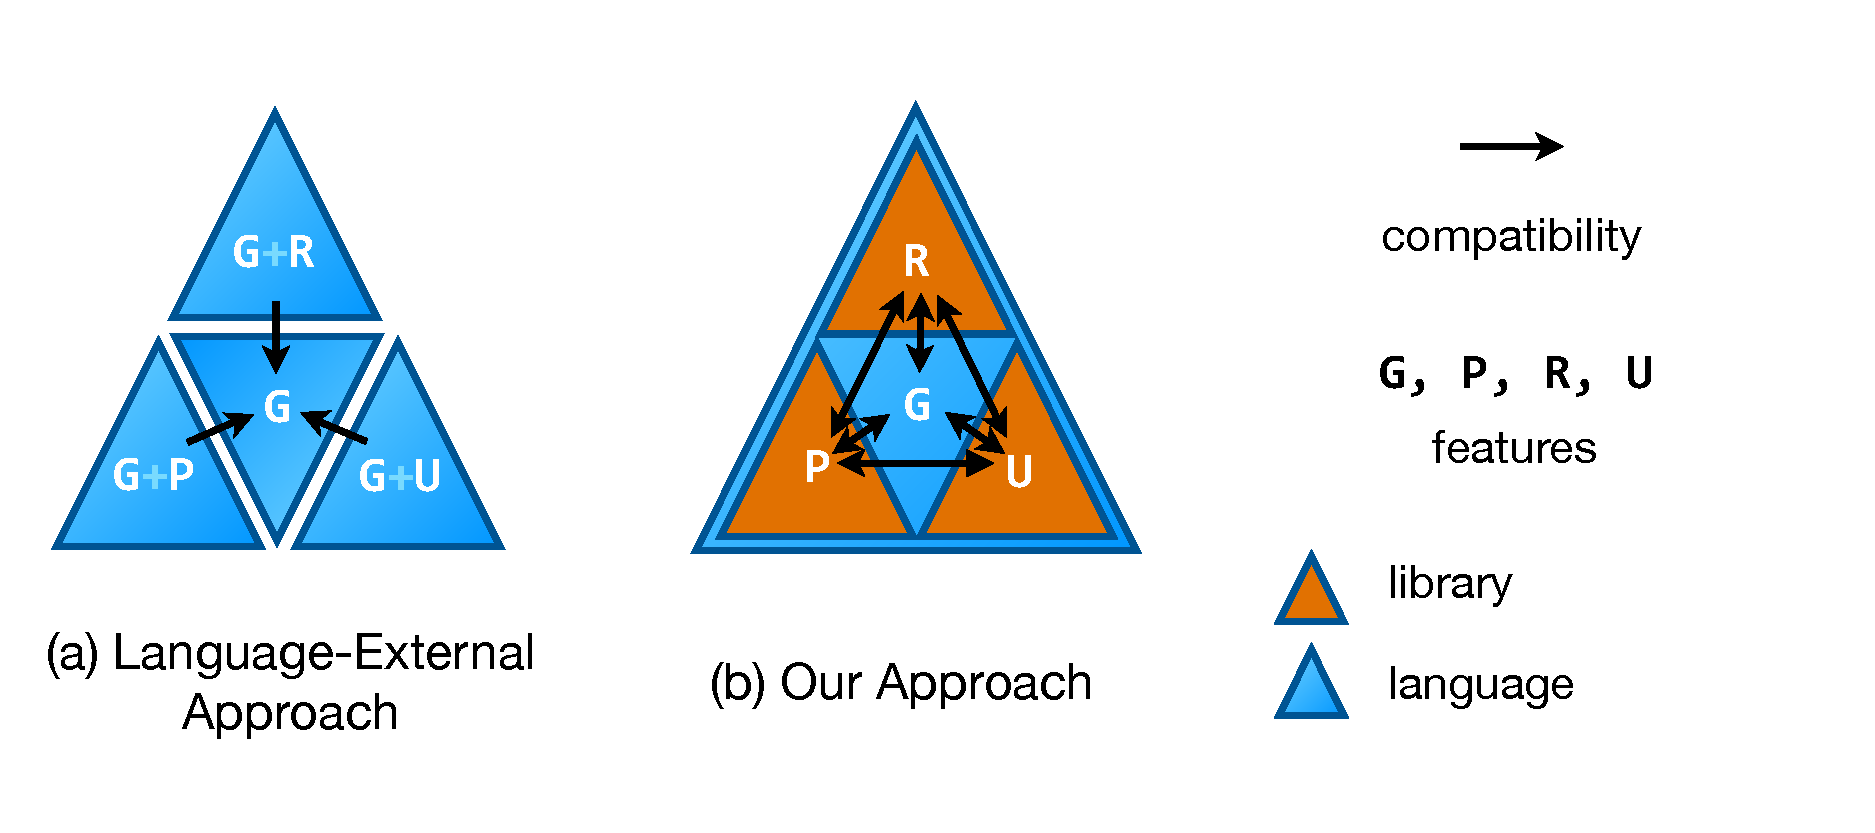
\includegraphics[scale=.48]{approaches.pdf}
% % \end{center}
% % \vspace{-20px}
% % \caption{\small (a) When taking a language-external approach, new features are packaged together into separate languages and tools. (b) We propose an approach where there is one extensible host language and the compile-time and edit-time logic governing new constructs is expressed within safely composable libraries.}
% % \label{approaches}
% % %\vspace{-10px}
% % \end{figure}
% %  %
% % % More specifically, there is no guarantee of \textbf{orthogonality} or even \textbf{interoperability}.% This has limited the broad adoption of these kinds of innovations.%This latter method couples the semantics of the feature to the implementation details of a particular tool. Because the use of one implementation entails a different semantics for the feature than another, the extended tool acts, \emph{de facto}, as a distinct system for our purposes. 

% % %\paragraph{Orthogonality} Features implemented by language-external means like these cannot be adopted individually, but instead are only available coupled to a fixed collection of other features. This makes adoption more costly when these incidental features are  not desirable or are insufficiently developed (``toy languages''), or when the features bundled with a different language or tool are simultaneously desirable. 

% % % Recent evidence indicates that this is one of the major barriers preventing research  from being driven into practice. For example, developers prefer high-level language-integrated parallel programming abstractions that provide  stronger semantic guarantees  \cite{cave2010comparing}, but library-based approximations are far more widely adopted because the ``parallel programming languages'' privilege only a few  specialized abstractions at the language level. In contrast, it is widely acknowledged that  different specialized abstractions are more appropriate in different situations \cite{Tasharofi:2013rc}. Moreover,  parallel programming is rarely the only relevant specialized concern. Support for regular expressions as above would be simultaneously desirable for processing large amounts of genomic data in parallel.% but using these features together in the same compilation unit would be difficult or impossible if implemented using language-external means. Indeed, switching to a ``parallel programming language'' would likely make it \emph{more} difficult to use regular expressions, as these are likely to be less well-developed in a specialized language than in an established general-purpose language.% This intuition was perhaps most succinctly expressed by a participant in a recent study by Basili et al. \cite{basili2008understanding}:  ``I hate MPI, I hate C++. [But] if I had to choose again, I would probably choose the same.'' %Similarly, a language and tools designed primarily to support regular expressions might make an interesting research project, but it would not be a suitable tool for writing large applications with more varied needs.

% % %\item Developing a new language and its associated tools places a significant development burden on providers who may wish only to promote a few core innovations, although tools like compiler generators, language workbenches and easy-to-extend tools can decrease this burden. 
% % %\item 

% % %Clients seem to prioritize the ability to choose different features for different portions of an application. 
% % %If calling between languages were safe and easy, then using a variety of specialized languages and associated tools might be less problematic. In fact, s
% % %Recognizing the limitations of relying on monolithic collection of primitives, some researchers have advocated instead for a model where multiple languages used within a single application, calling it the \emph{language-oriented approach} to software development \cite{languageoriented}. 

% % % \paragraph{Interoperability} Even in cases where, for each component of a software system, a programming system considered entirely satisfactory by its developers is available (e.g. a team goes through the trouble of implementing \verb|G+R+P| by reading papers about \verb|G+R| and \verb|G+P| and disentangling orthogonality-related issues), there remains a problem at any interface between  components written using a different combination of features. An interface that  externally exposes a specialized construct particular to one language (e.g. a function that requires a quantity having a particular unit of measure) cannot necessarily be safely and naturally consumed from another language (e.g. a parallel programming language). Tool support is also lost when calling into different languages. %We call this the \emph{interoperability problem}. % programs written by clients of a certain collection of features cannot always interface with programs written by clients of other features  in a safe, performant and natural manner.

% % % One strategy taken by proponents of a {language-oriented approach} \cite{journals/stp/Ward94} to partially address the interoperability problem is to  target an established intermediate language and use its constructs as a common language for communication between components written in different languages. Scala \cite{200464/IC} and F\# \cite{pickering2007foundations} are examples of prominent general-purpose languages that have taken this approach, and most DSL frameworks also rely on this strategy. As indicated in Figure \ref{approaches}a, this only enables interoperability in one direction. Calling into the common language becomes straightforward and safe, but calling in the other direction, or between the languages sharing the common target, does not, unless these languages are only trivially different from the common language. 

% % % %This approach only works well when new languages consist of constructs that can also be expressed safely and almost as naturally in the common language.
% % % %But many of the most innovative constructs found in modern languages (often, those that justify their creation) are difficult to define in terms of existing constructs in ways that guarantee all necessary invariants are statically maintained and that do not require large amounts boilerplate code and run-time overhead. 
% % % As a simple example with significant contemporary implications, F\#'s type system does not admit \verb|null| as a value for any type both defined and used within F\# code, but maintaining this sensible internal invariant still requires dynamic  checks because the stricter typing rules of F\# do not apply when F\# data structures are constructed by other languages on the Common Language Infrastructure (CLI) like C\# or SML.NET. This is not an issue exclusive to intermediate languages that make regrettable choices regarding \verb|null|, however. The F\# type system also includes support for checking that units of measure are used correctly \cite{syme2012expert, kennedy1994dimension}, but this more specialized static invariant is left entirely unchecked at language boundaries. Indeed, guidelines for F\# suggest that exposing functions that operate over values having units of measure, datatypes or tuples is not recommended when a component ``might be used'' from another language \cite{syme2012expert} because it is awkward to construct and consume these from other languages without the convenient primitive operations (e.g. pattern matching) and syntax that F\# includes. SML.NET prohibits exposing such types at component boundaries altogether. Moreover, it also cannot naturally consume F\# data structures, despite having a rather similar syntax and semantics in most ways (both languages directly descend from ML). 
% % %In Scala, traits that have default method implementations are difficult to implement from Java or other JVM languages and the workaround can break if the trait is modified \cite{scalatraitinterop}. 
% % %In some cases, desirable features must be omitted entirely due to concerns about interoperability. F\#, for example, aimed to retain source compatibility with Ocaml code, but due to the need for bidirectional interoperability with CLI languages, it does not support features like polymorphic variants, modules or functors \cite{ocaml-manual} because they have no apparent analogs in the type system of the CLI.
% % %\end{itemize}

% % %\subsection{Language-Integrated Approaches}\label{language-integrated-approaches}


% % %Such libraries have been called \emph{active libraries}  \cite{activelibraries}. %Features implemented within active libraries can be imported individually, unlike features implemented by external means, giving us a potential means to avoid the problems of orthogonality and interoperability just described.

% % % We must proceed with caution, however: critical issues having to do with {safety} must be overcome before language-integrated extension mechanisms can be introduced into a system. If too much control over  these core features of the system is given  to developers, the system's metatheory may become weak. 
% % % %For example, an extension could weaken important metatheoretic guarantees previously provided by the system. 
% % % For example, parsing ambiguities might arise if the syntax can be modified arbitrarily. Type safety  may not hold if the static and dynamic semantics of the language can be modified or extended arbitrarily from within libraries. Furthermore, even if extensions can be shown not to cause such problems in isolation, there may still be conflicts between extensions that could weaken their semantics, leading to subtle problems that only appear when two extensions are used together. %As a simple example, if two active libraries introduce the same syntactic form but back it with differing (but individually valid) semantics, this ambiguity  would only manifest itself when both libraries were imported within the same scope. %Resolving these kinds of ambiguities requires significantly more expertise with parser technology than using the syntax itself does. 
% % % These issues have plagued previous attempts to design language-integrated extensibility mechanisms.\todo{I can include a more detailed related work section if requested.}% We will briefly review some of these attempts below, then return to our approach.% To prevent them, our mechanisms will organize  extension logic around types to guarantee that extensions are both safe in isolation and also safely composable in any combination. 


% %  %This represents a minimalist approach to system design -- the conventional distinction between built-in and user-defined constructs is blurred and most features of the system are orthogonally implemented as {libraries}, rather than by the maintainers of the system.

% % %The mechanisms we describe will do so primarily by delimiting the scope of an extension to expressions of a single user-defined type or family of types. 

% % %This can be thought of as a more pernicious form of the conflict that arises when two globally-accessible constructs are given the same name. n languages without universal namespacing mechanisms (e.g. C, JavaScript, \LaTeX, ML and many others). 

% % %The extension mechanism\todo{elaborate on safety requirements + tension between expressiveness and safety, merge with next paragraph}. must be expressive enough to allow users to associate rich run-time, compile-time and edit-time behaviors with user constructs directly, while being sufficiently restrictive to maintain the global safety properties of the language and system as a whole, and to ensure that constructs cannot interfere with one another. 

\begin{figure}[p!]
\vspace{-25px}
\begin{lstlisting}
metasignature LTUPLE = metasig {
  ^\label{line:ltuplex-c-sig}^tycon c of ComponentSpec
  ^\label{line:intro-unlabeled-sig}^ana opcon intro_unlabeled of unit
  ^\label{line:intro-labeled-sig}^syn opcon intro_labeled of list(Lbl)
  ^\label{line:prj-sig}^syn opcon # of Lbl
  ^\label{line:conc-sig}^syn opcon + of unit
  ^\label{line:drop-sig}^syn opcon - of Lbl
}

^\label{line:ltplx-tsm-start}^syntax ltpl(L :: LTUPLE, param :: ComponentSpec) at L.c(param) {
  static fn ps => (* 
    - elaborates {e_1, ..., e_n} to 
        L.intro_unlabeled () (e_1; ...; e_n)
    - elaborates {lbl1 => e_1, ..., lbln => e_n} to 
        L.intro_labeled [lbl1, ..., lbln] e_1 ... e_n
  *)
}^\label{ltplx-tsm-end}^

metamodule Ltuple :: LTUPLE = metamod {
  ^\label{line:c-start}^(* translate labeled tuple types to nested products *)
  tycon c {
  	(* type translation generator: *)
  	static fn (param :: ComponentSpec) :: ITy => fold (comp_spec_to_tuples param)
      `SCSSunitECSS`
      (fn ((lbl, ty), cur_ty_trans) => `SCSStrans(ECSStySCSS) * %ECSScur_ty_trans`)
  }^\label{line:c-end}^

  ^\label{line:introul-start}^ana opcon intro_unlabeled {
  	(* translate intro operator to nested pairs *)
  	static fn (ty :: Ty, op_param :: unit, args :: list(Arg)) :: IExp => tycase(ty) {
        c(ty_param) => (fold (zipExact (comp_spec_to_tuples ty_param) args)
      	  `SCSS()ECSS`
          (fn (((lbl, ty), arg), cur_trans) => `SCSS(%{ECSSana(arg, ty)SCSS}, %ECSScur_transSCSS)ECSS`)
        )
      | _ => raise TyErr("...")
    }
  }^\label{line:introul-end}^

  ^\label{line:introl-start}^syn opcon intro_labeled {
  	static fn (op_param :: list(Lbl), args :: list(Arg)) :: Ty * IExp => 
      (* ... similar to intro_unlabeled but reorder first ... *)
  }^\label{line:introl-end}^

  ^\label{line:prj-start}^syn opcon # {
  	static fn (op_param :: Lbl, args :: list(Arg)) :: Ty * IExp =>  
      (* ... generate the appropriate n-fold projection ... *)
  }^\label{line:prj-end}^

  ^\label{line:ltpl-conc-start}^syn opcon + {
  	static fn (op_param :: unit, args :: list(Arg)) :: Ty * IExp => 
      (* generate the new type and combine the two nested tuples *)
  }^\label{line:ltpl-conc-end}^

  ^\label{line:ltpl-drop-start}^syn opcon - {
  	static fn (op_param :: Lbl, args :: list(Arg)) :: Ty * IExp => 
      (* generate the new type and drop the appropriate component *)
  }^\label{line:ltpl-drop-end}^
} with syntax ltpl^\label{line:ltplx-annotation}^
(* synonyms used in Sec. 5.1 *)
^\label{line:tycon-synonym}^let tycon ltuple = Ltuple.c
let opcon # = Ltuple.#
let opcon ltuple+ = Ltuple.+ 
let opcon ltuple- = Ltuple.-
\end{lstlisting}
\caption{Using metamodules to define the type structure of labeled tuple types.}
\label{fig:ltuplex}
\end{figure}
% !TEX root = omar-thesis-proposal.tex
\subsubsection{Background}\label{alibs}\label{background}
The term \emph{active libraries} was first introduced by Veldhuizen et al. \cite{activelibraries, active-libraries-thesis} to describe ``libraries that take an active role in compilation, rather than being passive collections of subroutines''. The authors suggested a number of reasons libraries might benefit by being able to influence the programming system at compile-time or edit-time, including high-level program optimization, checking programs for correctness against specialized criteria, reporting domain-specific errors and warnings, and ``rendering domain-specific textual and non-textual program representations and for interacting with such representations'' (anticipating interactions between libraries and tools other than just the compiler). 

% This stuff isn't actually hooking into the compiler...
The first concrete realizations of active libraries in statically typed settings, prompting the introduction of the term, were libraries that performed domain-specific program optimization at compile-time by exploiting language mechanisms that allow for limited compile-time computation. A prominent example in the literature is Blitz++, a library that uses C++ template metaprogramming to optimize compound operations on vectors and matrices by eliminating intermediate allocations \cite{veldhuizen2000blitz++}. Although this and several other interesting optimizations have been shown possible by this technique, its expressiveness is fundamentally limited because template expansion allows for only the substitution of compile-time constants into pre-written code, and template metaprograms are notoriously difficult to read, write, debug and reason about (see discussion in \cite{Robison:2001:IEC:376656.376751}). %They are, however, composable, because templates are associated with a single function or class, and  the only metatheoretic issue is that template expansion can be non-terminating.

More powerful and direct compile-time \emph{term rewriting mechanisms} available in some languages can also be used for optimization, as well as for introducing specialized error checking logic and extending a language with new abstractions. These mechanisms are highly expressive because they allow users to programmatically manipulate syntax trees directly, but they suffer from problems of composability and safety. For example, compile-time macros, such as those in MetaML \cite{Sheard:1999:UMS}, Template Haskell \cite{SheardPeytonJones:Haskell-02} and Scala \cite{scala-macros}, take full control over all of the code that they enclose. This can be problematic, however, as outer macros can interfere with the functionality of inner macros. Moreover, once a value escapes a macro's scope, there is no way to rely on the guarantees and features that were available within its scope, because the output of a macro is simply a value in the underlying language (a problem fundamentally related to the problem of relying on a common intermediate language,  described in Section \ref{external-approaches}). Thus, macros can be used to automate code generation, but not to truly extend the semantics of a language. It can also be difficult to reason about the semantics of code when any number of enclosing macros may be manipulating it, and to build tools that operate robustly in their presence.

Some term rewriting systems replace the explicitly delimited scoping of macros with global pattern-based dispatch. Xroma (pronounced ``Chroma''), for example, is designed around active libraries and allows users to insert custom rewriting passes into the compiler from within libraries \cite{activelibraries}. Similarly, the derivative of Haskell implemented by the Glasgow Haskell Compiler (GHC) allows providers to introduce custom compile-time term rewriting logic if an appropriate flag is passed in \cite{jones2001playing}. In both cases, the user-defined logic can dispatch on arbitrary patterns of code throughout the component or program the extension is activated within, so these mechanisms are highly expressive and avoid some of the difficulties of explicitly invoked macros. But libraries containing such global rewriting logic cannot be safely composed because two different libraries may attempt to rewrite the same piece of code differently. It is also difficult to guarantee that such logic is correct and difficult to reason about code when simply importing a library can change the semantics of the program in a highly non-local manner.
% http://www.haskell.org/ghc/docs/latest/html/users_guide/rewrite-rules.html

Another example of an active library approach to extensibility is SugarJ \cite{erdweg2011sugarj} and other languages generated by Sugar* \cite{erdweg2013framework}, like SugarHaskell \cite{erdweg2012layout}. These languages permit libraries to extend the base syntax of the core language in a nearly arbitrary manner, and these extensions are imported transitively throughout a program. Unfortunately, this flexibility means that  extensions are also not safely composable. For example, a library that defines a literal syntax for HTML would conflict with another that defines a literal syntax for XML because they define differing semantics for some of the same syntactic forms. If SugarJ was used by two different regular expression engines to provide literal syntax for regular expression patterns, there could easily be conflicts at link-time because both will introduce many of the same notations but back them with differing implementations. 
And again, it is difficult to predict what an unfamiliar piece of syntax desugars into, leading to difficulties reading and reasoning about code.

%Another example comes from the Tau package for tuning and analyzing parallel programs, which allows libraries to instrument themselves declaratively so that internal details can be hidden from users of the tool \cite{tau}. 

%The researchers behind these tools often claim that such conflicts are rare. There have, to our knowledge, been no studies of this claim. Nevertheless, the core fact remains: conflicts can arise, which makes it difficult to rely on such libraries 

%There also does not appear to be a clear, well-founded theoretical foundation for this approach, nor for active libraries in general.

%\todo{Smooth this transition}Developers specify type-specific compile-time and edit-time features by equipping type families, when they are defined, with functions written in an appropriate metalanguage. These are selectively invoked by tools, such as the parser, type checker, translator and editor, when they work with expressions of that type, and only in those situations.

%\subsection{Example: First-Class Natural Numbers}
%To make our approach more concrete and emphasize its foundational character, let us begin with a very simple example, first-class natural numbers. If a programming system included first-class support for natural numbers, it might support behaviors like the following:
%
%\begin{enumerate}
%\item type checking rules that constrain uses of the three operators associated with the $\nat$ type, as defined in G\"{o}del's System \textbf{T} \cite{tapl}: $\natz$, $\nats{e}$ and $\natrec{e_1}{e_2}{e_3}$\todo{phrasing of his}
%\item type checker error messages that provide domain-specific assistance, like detecting when the trailing $\textbf{z}$ in a constant has been omitted: \todo{phrasing / merge this into 1?}
%\begin{verbatim}
%    s(s(s))
%        ^ (Line 1, Character 5)
%    Error: Operator s requires 1 argument of type nat. Provided 0 arguments.
%    Did you mean s(z)?
%\end{verbatim}
%\item translation into an efficient integer representation at run-time
%\item syntax support \todo{elaborate on syntax support for nat literals}
%\item editor support, such as the ability to instantiate nat constants more easily \todo{elaborate on this / reference Graphite section}
%%generate statistical predictions useful for code completion (e.g. biasing smaller constants) and other editor interactions, customized syntactic/visual representations and so on.
%\end{enumerate}
%


%\section{Related Work}
%We review existing approaches that are available to researchers and domain experts who wish to develop novel constructs below.
%
%\subsection{Language-Oriented Approaches}
%\subsubsection{Language Frameworks}
%A number of tools have been developed to assist with this task of developing new languages and their associated tools, including compiler generators, language workbenches and domain-specific language frameworks (see \cite{fowler2010domain} for a review). In some cases, these tools allow language features to be defined modularly and composed differentially to produce a variety of different languages. To our knowledge, none of these mechanisms guarantee that any combination of features can be safely composed, nor do they guarantee safety properties about the resulting languages. User-defined code is still ultimately compiled against a particular language, and because language composition cannot be automatic or guaranteed safe, interoperability with code written in other languages is thus limited by the difficulties described above despite the modular construction.
%
%\subsubsection{Extensible Compilers and Tools}
%A related methodology is to implement language features as compiler and tool extensions directly. A number of extensible compilers have been developed to support this approach (see \cite{clements2008comparison}). As with language frameworks, this approach can lead to \emph{de facto} implementation of a new language, since user libraries must be compiled against a particular combination of extensions, and these extensions cannot be guaranteed to compose in general. Moreover, a language may have multiple competing compilers and other tools. By relying on implementation-specific features of a single tool to define core semantics and behaviors, the clean conceptual separation between languages and tools is broken, leading to compatibility issues and hard-to-anticipate behaviors for user code. We argue that this approach should be considered harmful.
%
%\subsection{Library-Oriented Approaches}
%\subsubsection{Embedded DSLs}
%Embedded domain-specific languages are languages that creatively repurpose existing language constructs to create interfaces that resemble those of a distinct language. In languages with rich type systems, such as Haskell, this approach can be quite successful (e.g. \cite{svensson2011obsidian}). Ultimately, however, this approach is limited by the host system, and as discussed in Section 2, thus limits experts who want to express particularly novel constructs, relative to the host language. 
%
%\subsubsection{Term Rewriting Systems}
%Many languages and tools allow developers to rewrite expressions according to custom rules. These can broadly be classified as {\it term rewriting systems}. Macro systems, such as those characteristic of the LISP family of languages \cite{mccarthy1978history}, are the most prominent example. Some compile-time metaprogramming systems also allow users to manipulate syntax trees (e.g. MetaML \cite{Sheard:1999:UMS}), and external rewrite systems also exist for many languages. These systems are expressive if used correctly, but verifying correctness and non-interference properties is difficult for the same reason. Manipulating source trees directly is a complex task, even in languages with simple grammars like LISP. Finally, term rewriting systems focus on rewriting terms to support alternative language semantics but do not intrinsically support extensions that cover the full programming system.
%
%\subsubsection{Active Libraries}
%Active libraries, as proposed by Czarnecki et al. \cite{activelibraries}, ``are not passive collections of routines or objects, as are traditional libraries, but take an active role in generating code''. They go on to suggest a number of areas in which the library could interact with the programming system, including optimizing code, checking source code for correctness, reporting domain-specific errors and warnings, and ``rendering domain-specific textual and non-textual program representations and for interacting with such representations''. 
%
%This paper was largely a proposal. The concrete implementations of this concept have largely been term rewriting systems described above. One prominent example within the active libraries literature is Blitz++, which uses the C++ template expansion system as a metalanguage to support optimizations of array operations. An example of tool support comes from the Tau package for tuning and analyzing parallel programs. Tau allows libraries to instrument themselves declaratively to hide internal details and complex internal representations from users. A more extensive system with support for active libraries is Xroma. Xroma allows users to provide annotations that intercept compilation of a component at various stages of compilation to support rewriting, custom error handling and custom error checking. The approach taken by Xroma, by still requiring direct syntax manipulation and allowing arbitrary interception, is flexible but not compositional, and generally more complex than may be necessary. There also does not appear to be a clear, well-founded theoretical foundation for this approach, nor for active libraries in general.

%\subsection{Type-Level Computation} %Haskell, Ur and $\Omega$mega
%System XX with simple case analysis provides the basis of type-level computation in Haskell (where type-level functions are called type families \cite{Chakravarty:2005:ATC}). Ur uses type-level records and names to support typesafe metaprogramming, with applications to web programming \cite{conf/pldi/Chlipala10}. $\Omega$mega adds algebraic data types at the type-level, using these to increase the expressive power of algebraic data types at the expression level \cite{conf/cefp/SheardL07}. Dependently-typed languages blur the traditional phase separation between types and expressions, so type-level computation is often implicitly used (though not always in its most general form, e.g. Deputy \cite{conf/icfp/ChenX05}, ATS \cite{conf/esop/ConditHAGN07}.)

%\subsubsection{Run-Time Indirection}
%{\it Operator overloading} \cite{vanWijngaarden:Mailloux:Peck:Koster:Sintzoff:Lindsey:Meertens:Fisker:acta:1975} and {\it metaobject dispatch} \cite{Kiczales91} are run-time protocols that translate operator invocations into function calls. The function is typically selected according to the type or value of one or more operands. These protocols share the notion of {\it inversion of control} with type-level specification. However, type-level specification is a {\it compile-time} protocol focused on enabling specialized verification and implementation strategies, rather than simply enabling run-time indirection.

%\subsection{Specification Languages}
%Several {\it specification languages} (or {\it logical frameworks}) based on these theoretical formulations exist, including the OBJ family of languages (e.g. CafeOBJ \cite{Diaconescu-Futatsugi01}). They provide support for verifying a program against a language specification, and can automatically execute these programs as well in some cases. The  language itself specifies which verification and execution strategies are used.
%
%Type-determined compilation takes a more concrete approach to the problem, focusing on combining {\it implementations} of different\- logics, rather than simply their specifications. In other words, it focuses on combining {\it type checkers} and {\it implementation strategies} rather than more abstract representations of a language's type system and dynamic semantics. In Section 4, we outlined a preliminary approach based on proof assistant available for the type-level language to unify these approaches, and we hope to continue this line of research in future work.
%

% !TEX root = omar-thesis-proposal.tex
\section{Active Types}\label{contributions}
The language-integrated extension mechanisms that we will introduce in this thesis are designed to be highly \textbf{expressive}, permitting library-based implementations of features comparable to the built-in features found in modern programming systems, but without the kinds of \textbf{safety} problems that have been an issue in previous mechanisms, as described above. We also aim to maintain the ability to understand and reason locally about code. This is accomplished by organizing extension logic around types and scoping it to or around expressions of the type it is associated with, rather than applying it globally or within an explicitly delimited scope as in previous mechanisms. 

To motivate this approach, let us return to our example of regular expressions. Observe that every feature described in Sec. \ref{regex} relates specifically to how terms  classified by a single user-defined type or family of types should behave. In fact, nearly all the features relate to the type representing regular expression patterns (let us call it \verb|Pattern|\footnote{We should note at the outset that to fully prevent conflicts between libraries, naming conflicts must also be avoided. Suitable namespacing mechanisms (e.g. URI-based schemes, as Java uses) are already widely used in practice  and will be assumed implicitly whenever needed.}). Feature 1 calls for specialized syntax for the introductory form for this type. Features 2a and 2b relate to its static and dynamic semantics. Feature 3 is about its edit-time behavior. The remaining feature, 2c, also relates to the semantics of a single family of types: \verb|StringIn[r]|, which classifies strings known to be in the language of the statically-known regular expression \verb|r|. It is exclusively when editing or compiling expressions of the associated type that the logic in Sec. \ref{regex}  needs to be considered. 

Indeed, this is not a property unique to our chosen example, but a commonly-seen pattern in programming language design. The semantics of a programming language or logic is often organized around its types (equivalently, its propositions). In two major textbooks about programming languages, TAPL \cite{tapl} and PFPL \cite{pfpl}, most chapters describe the semantics and metatheory of a few new types and their associated primitive operations without reference to other types. The composition of the types and associated operations from different chapters into complete languages is a language-external operation. For example, in PFPL, the notation $\mathcal{L}$\{$\rightarrow$ \verb|nat| \verb|dyn|\} represents a language composed of the arrow ($\rightarrow$), \verb|nat| and \verb|dyn| types and their associated operators. Each of these are defined in separate chapters, and it is generally left unstated that the semantics and metatheory developed separately will compose without trouble (justified by the fact that, upon careful examination, it is indeed the case that almost any combination of types defined separately in PFPL can be combined to form a language with little trouble). 

This ubiquitous type-oriented organization suggests a principled language-integrated alternative to the mechanisms described in Section \ref{alibs} that preserves much of their expressiveness but eliminates the possibility of conflict and makes it easier to reason locally about a piece of code: associating extension logic directly with a single type (or family of types) and scoping it to affect only expressions classified by that type (or by a type in that family). This guarantees that different extensions don't have overlapping scope, preventing a range of common conflicts. By constraining the extension logic itself by various means we will show that the system as a whole can also maintain many other important safety and non-interference properties that have not previously been achieved. We call types with such logic associated with them \emph{active types} and systems that support them \emph{actively-typed programming systems}. 

\subsection{Proposed Contributions}
This thesis will introduce several language-integrated extensibility mechanisms, each based on active types, that give providers control over a different aspect of the system from within libraries (that is, in a decentralized manner). In each case, we will show that the system remains fundamentally safe and that extensions cannot interfere with one another. We will also discuss various points in the design space related to extension correctness (as distinct from safety, which is guaranteed even if an incorrect extension is used). To justify the  expressiveness of each approach, we will give a number of examples of non-trivial features that are, or would need to be, built into other systems, but that can be expressed within libraries using our mechanisms. To help us gather a broad, unbiased collection of examples and demonstrate the scope and applicability of our approaches in practice, we conduct empirical studies.

We begin in Sec. \ref{aparsing} by considering \textbf{syntax}. The availability of specialized syntax can bring numerous cognitive benefits \cite{green1996usability}, and discourage the use of problematic techniques like using strings to represent structured data \cite{Bravenboer:2007:PIA:1289971.1289975}. But allowing library providers to add arbitrary new syntactic forms to a language's grammar can lead to interference issues, as described above. We observe that many syntax extensions are motivated by the desire to add alternative  introductory forms (a.k.a. \emph{literal forms}) for a particular type. For example, regular expression pattern literals as described in Sec. \ref{regex} are an introductory form for the \verb|Pattern| type.  In the mechanism we introduce, syntax extensions are associated directly with a type and are active only where an expression of that type is expected (shifting part of the burden of parsing into the typechecker). This avoids extension interference problems because the base grammar of the language is never extended directly. We call such an extension a \emph{type-specific language (TSL)} and introduce TSLs in the context of a new language, Wyvern. We begin by showing how interference issues between the base language and the TSL syntax can be avoided by either introducing minor syntactic constraints on the body of a literal or by using a novel layout-delimited literal form. We then develop a formal semantics, basing it on work on bidirectional type systems and elaboration semantics, and introduce a novel mechanism that statically prevents unsafe variable capture and shadowing by extensions (providing a form of \emph{hygiene}). Finally, we conduct a corpus analysis to examine this technique's expressiveness, finding that a substantial fraction of string literals in existing code could be replaced by TSL literals.

Wyvern has an extensible syntax but a fixed general-purpose static and dynamic semantics. The general-purpose abstraction mechanisms we have included in Wyvern are powerful, and implementation techniques for these are well-developed, but there remain situations where providers may wish to extend the \textbf{semantics} of a language directly, by introducing new primitive types and operations. Examples of type system extensions that require this level of control abound in the research literature. For example, to implement the features in Sec. \ref{regex}, new logic must be added to the type system to statically track information related to backreferences (feature 2b, see \cite{spishak2012type}) or to execute a decision procedure for language inclusion when determining whether a coercion is possible (feature 2c, see \cite{fulton-thesis}). We discuss more examples from the literature where general-purpose abstraction mechanisms proved inadequate and researchers had to turn to language-external approaches in Sec. \ref{att}. To support these more advanced use cases in a decentralized manner, we next develop language-integrated mechanisms for implementing semantic extensions, while leaving the syntax fixed. We begin in Sec. \ref{foundations} with a type theoretic treatment, specifying an ``actively typed'' lambda calculus called @$\lambda$. By beginning from first principles, we are able to cleanly state and prove the key safety and non-interference theorems and examine the connections between active types and several prior notions, including type-level computation, typed compilation and abstract types. We then go on in Sec. \ref{ace} to demonstrate the expressiveness of this mechanism by designing and implementing a full-scale actively typed language, Ace. Interestingly, Ace is itself bootstrapped as a library within an existing language, Python. We discuss how we accomplish this, relate Ace to the core calculus and implement a number of powerful primitives from existing languages as libraries, giving examples from a variety of paradigms, including low-level parallel programming, functional programming, object-oriented programming and specialized domains, like regular expression types.

Finally, in Sec. \ref{acc}, we will show how \textbf{editor services} can be implemented from within active libraries, by a technique we call \emph{active code completion}. To provide a new editor service, providers associate
specialized user interfaces, called \emph{palettes}, with types. Clients discover and invoke palettes from the code completion menu at edit-time, populated according to the expected type at the cursor (a protocol similar to the one we use for syntax extensions in Wyvern). When the interaction between the client and the palette is complete, the palette generates a term of the type it is associated with based on the information received from the user. Using several empirical
methods, we surveyed the expressive power of this approach and developed design criteria. Based on these initial studies, we then developed an active code completion system for Java called Graphite. Using Graphite,
we implemented a palette for working with regular expressions and conduct a small study that demonstrates the usefulness of this approach.

Taken together, these mechanisms demonstrate that actively-typed mechanisms can be introduced throughout a programming system to allow users to extend both its compile-time and edit-time semantics from within libraries, without  weakening the safety guarantees that the system provides. They also further reinforce the idea that types are a natural organizational unit for defining programming system features and show how a type-oriented approach can make it easier to guarantee that the features will be safely composable in any combination. By implementing our techniques within a variety of different host systems, we demonstrate that actively-typed mechanisms are relevant across traditional paradigms. In the future, we anticipate developing a programming system that will bring together several actively-typed mechanisms, organized around a minimal, well-specified and formally verified core, where nearly every feature is specified, implemented and verified in a decentralized manner and distributed as a library. 

%
%This suggests that a natural place where these features can be defined is in the library containing the declaration of \verb|Pattern| itself, rather than in the language and tool implementations. An \emph{actively-typed} definition of \verb|Pattern| would thus be equipped with	 functions that described how the parser (item 1), type checker (item 2), translator (item 3) and editor (item 4) should operate when working with expressions of type \verb|Pattern|. We can abstractly denote this declaration, as it would exist within a user-defined library, as follows:
%\begin{equation*}
%{\sf type}~Pattern[f_{\text{editor}}]\{
%\textbf{z}[f_{\text{resolve-z}}, f_{\text{compile-z}}], 
%\textbf{s}[f_{\text{resolve-s}}, f_{\text{compile-s}}], 
%\textbf{natrec}[f_{\text{resolve-rec}}, f_{\text{compile-rec}}]\}
%\end{equation*}
%
%When type checking an expression like $\nats{\nats{\natz}}$, the type checker delegates to the user-provided type-level function $f_{\text{resolve-s}}$. This function would be tasked with assigning a type to expression as a whole, given information including the \emph{types} (but not necessarily the full syntax trees) of all its subexpressions, or if a type cannot be assigned, producing a specific error message. Similarly, the compiler calls the $f_{\text{compile-s}}$ function to determine a representation in the target language for the expression, checking to ensure that it is well-formed and type-correct with respect to the target type system. Finally, elements of the editor may call into the $f_{\text{editor}}$ function (or one of several such functions, more generally) to control behaviors like code completion and code prediction when an expression of type $\nat$ is being entered. 
%
%Note that these functions are \emph{not} to be conflated with methods or run-time functions -- they are functions written in a type-level language that are called at compile-time and edit-time to define the basic behaviors associated with the type that they are associated with.
%
%\subsection{Characteristics of an Actively-Typed Programming System}
%An actively-typed programming system can be characterized by its choice of type-level language, source grammar, target language and dispatch protocols.
%
%\paragraph{Type-Level Language} The type-level language is the language within which the type definitions and the functions that define their behaviors are defined. This language must be constrained so that different definitions do not interfere with one another and so that desirable safety properties for the system as a whole are maintained, as we discuss below.
%
%\paragraph{Source Language} The source language is the language with which run-time behavior is defined. In our example above, terms like $\nats{\nats{\natz}}$ are part of the source language. In the purest case, the source language is simply a grammar; its semantics are given entirely by active type specifications.
%
%\paragraph{Dispatch Protocol} For each syntactic form in the source language, there is a dispatch protocol that determines which type is delegated responsibility over it, and which specific function(s) are called for each behavior the system supports. This fixed protocol makes it possible for users to predict the meaning of a construct using information local to the term, a key differentiator of this approach compared to term-rewriting systems where there can be action at a distance.
%
%\paragraph{Target Language} The target language is the language that the front-end compilation phase of the system targets. The limitations and constraints imposed by the target language are final, because all constructs ultimately translate into terms in the target language. In other words, active type specifications can only add additional invariants to the language; they cannot violate invariants imposed by the target language.

%\subsection{Research Challenges}
%The example of natural numbers given above is relatively simple, and the solution we outline remains abstract. A key challenge is then to demonstrate that this approach is able to express the behaviors of more sophisticated language constructs that span diverse problem domains, and be implemented in the context of a realistic collection of tools. The resulting system should be usable by developers who lack the expertise needed to define new language constructs themselves.
%
%Simultaneously, we must also demonstrate that this model is well-motivated theoretically, place it within the broader context of the theory of typed programming languages, and demonstrate that it is possible for desirable system safety properties to be maintained. In particular, we are interested in properties like:
%
%\begin{itemize}
%\item Correctness of active type specifications, so that users of a library need not be forced to debug errors arising within the specifications themselves.
%\item Correctness of translations, so that the results of translation are guaranteed to be well-typed and consistent with respect to the target language.
%\item Termination of active type specifications, so that evaluation of the type-level functions cannot cause the compiler or editor to hang.
%\item Composability of active type specifications, so that the behaviors defined by one type cannot interfere with those defined by another, no matter the order in which they are imported. This property is essential if we wish to place these specifications within normal libraries.
%\end{itemize}



% % !TEX root = omar-thesis-proposal.tex
\section{Tycon-Specific Languages (TSLs)}\label{aparsing}
Many abstractions can be seen, semantically, as modes of use of general-purpose constructs like sums and products. 
%By using a general-purpose construct to define a data structure, one immediately benefits from a body of useful operators, established reasoning principles, well-optimized implementations and tool support. 
For example, lists can be defined using a more general mechanism for defining polymorphic recursive sum types by observing that a list can either be empty, or be broken down into a product of the \emph{head} element and the \emph{tail}, another list. In an ML-like language, this would be written as a datatype:
\begin{lstlisting}[numbers=none]
datatype 'a list = Nil | Cons of 'a * 'a list
\end{lstlisting}
By defining type constructors like \li{list} in terms of these general purpose semantic mechanisms, we immediately know how to reason about them (here, by structural induction) and examine them (by pattern matching). They are already well optimized by compilers and benefit from general-purpose editor support as well. %The programmer only needs to provide an encoding of the structure of lists; the semantics and implementation are filled in by the general-purpose abstraction mechanism.
While this is all quite useful, the associated general-purpose concrete syntax is often less than ideal. For example, few would claim that writing a list of numbers as a sequence of \li{Cons} cells is convenient:
\begin{lstlisting}[numbers=none]
Cons(1, Cons(2, Cons(3, Cons(4, Nil))))
\end{lstlisting}

Because lists are a common data structure, many languages build in \emph{literal syntax} for introducing them, e.g. \li{[1, 2, 3, 4]}. This syntax is semantically equivalent to the general-purpose syntax shown above, but brings cognitive benefits by drawing attention to the content of the list, rather than the nature of the encoding. Using terminology from Green's cognitive dimensions of notations \cite{green1996usability}, it is more \emph{terse}, \emph{visible} and \emph{maps more closely} to the intuitive notion of a list. Stoy, in discussing the value of good notation, writes \cite{stoy1977denotational}:
\begin{quote}\emph{A good notation thus conceals much of the inner workings behind suitable abbreviations, while allowing us to consider it in more detail if we require: matrix and tensor notations provide further good examples of this. It may be summed up in the saying: ``A notation is important for what it leaves out.''}\end{quote}

List, number and string literals are nearly ubiquitous features of modern languages. Some languages additionally  build in  specialized notation for other common data structures (like maps, sets, vectors and matrices), data formats (like XML and JSON), query languages (like regular expressions and SQL), markup languages (like HTML and Markdown) and many other types of data. For example, a language with built-in notation for HTML and SQL, supporting type-safe \emph{splicing} via curly braces, might define:
\begin{lstlisting}
let webpage : HTML = SHTML<html><body><h1>Results for {EHTMLkeywordSHTML}</h1>
  <ul id="results">{EHTMLto_list_items(query(db, 
    SSQLSELECT title, snippet FROM products WHERE {ESQLkeywordSSQL} in titleESQL)SHTML}
  </ul></body></html>EHTML
\end{lstlisting}
as more concise and natural shorthand for:
\begin{lstlisting}
let webpage : HTML = HTMLElement(Dict.empty(), [BodyElement(Dict.empty(),
  [H1Element(Dict.empty(), [TextNode($\texttt{"}$SSTRResults for $\texttt{"}$ESTR + keyword)]), 
  ULElement((Dict.add Dict.empty() ($\texttt{"}$SSTRid$\texttt{"}$ESTR, $\texttt{"}$SSTRresults$\texttt{"}$ESTR)), to_list_items(query(db, 
    SelectStmt([$\texttt{"}$SSTRtitle$\texttt{"}$ESTR, $\texttt{"}$SSTRsnippet$\texttt{"}$ESTR], $\texttt{"}$SSTRproducts$\texttt{"}$ESTR, 
      [WhereClause(InPredicate(StringLit(keyword), $\texttt{"}$SSTRtitle$\texttt{"}$ESTR))]))))]]]
\end{lstlisting}

When a specialized notation like this is not available, but this equivalent general-purpose notation, which in essence captures only the abstract syntax of languages like HTML and SQL, is unsatisfying, developers typically turn to run-time mechanisms to make constructing data structures more convenient. Among the most common strategies across language paradigms in these situations is to simply use a string representation that is parsed at run-time.% Developers across language paradigms frequently write examples like the above as:
\begin{lstlisting}
let webpage : HTML = parse_html($\texttt{"}$SSTR<html><body><h1>Results for ESTR$\texttt{"}$ + keyword + $\texttt{"}$SSTR</h1>
  <ul id=\$\texttt{\color{cyan}"}$results\$\texttt{\color{cyan}"}$>$\texttt{"}$ESTR + to_string(to_list_items(query(db, parse_sql(
  	$\texttt{"}$SSTRSELECT title, snippet FROM products WHERE '$\texttt{" + keyword + "}$' in title$\texttt{"}$ESTR)))) + 
  $\texttt{"}$SSTR</ul></body></html>$\texttt{")}$
\end{lstlisting}

Though recovering some of the notational convenience of the literal version, it is still more awkward, requiring explicit conversions to and from structured representations (\li{parse_html} and \li{to_string}, respectively) and escaping when the syntax of the language interferes with the syntax of string literals (line 2). Code like this also causes a number of problems beyond cognitive load. Because parsing occurs at run-time, syntax errors will not be discovered statically, causing potential problems in production scenarios. Run-time parsing also incurs performance overhead, particularly relevant when code like this is executed often (as on a heavily-trafficked website). But the most serious issue with this code is that it is fundamentally insecure: it is vulnerable to cross-site scripting attacks (line 1) and SQL injection attacks (line 3). For example, if a user entered the keyword \li{'; DROP TABLE products --}, the entire product database could be erased. These attack vectors are considered to be two of the most serious security threats on the web today \cite{owasp2013}. Although developers are cautioned to sanitize their input, it can be difficult to verify that this was done correctly throughout a codebase. The best way to avoid these problems today is to avoid strings and insist on structured representations, despite the inconvenient notation.

Unfortunately, situations like this, where maintaining strong correctness, performance and security guarantees entails significant syntactic overhead, causing developers to turn to worse solutions that are more convenient, are quite common. To emphasize this, let us return to our running example of pattern literals. A small regular expression like \verb!(\d\d):(\d\d)\w*((am)|(pm))! might be written using general-purpose notation as:
\begin{lstlisting}
Seq(Group(Seq(Digit, Digit), Seq(Char($\texttt{"}$SSTR:ESTR$\texttt{"}$), Seq(Group(Seq(Digit, Digit)), 
  Seq(ZeroOrMore(Whitespace), Group(Or(Group(Seq(Char($\texttt{"}$SSTRaESTR$\texttt{"}$), Char($\texttt{"}$SSTRmESTR$\texttt{"}$))), 
  Group(Seq(Char($\texttt{"}$SSTRpESTR$\texttt{"}$), Char($\texttt{"}$SSTRmESTR$\texttt{"}$))))))))))
\end{lstlisting}
This is clearly more cognitively demanding, both when writing the regular expression and when reading it. Among the most common strategies in these situations, for users of any kind of language, is again to simply use a string representation that is parsed at run-time:
\begin{lstlisting}
rx_from_str($\texttt{"}$SSTR(\\d\\d):(\\d\\d)\\w*((am)|(pm))ESTR$\texttt{"}$)
\end{lstlisting}
%%
%%For example, in languages without SQL literals, developers can implement a builder pattern:
%%\begin{lstlisting}
%%new SQLQuery().SELECT("*").FROM("table").WHERE("username").Eq(username)
%%\end{lstlisting}
This is problematic, for all of the reasons described above: excessive conversions between representations, interference issues with string syntax, correctness problems, performance overhead and security issues.

Today, supporting new literal syntax within an existing programming language requires the cooperation of the language designer. This is primarily because, with conventional parsing strategies, not all notations can unambiguously coexist, so a designer is needed to make choices about which syntactic forms are available and what their semantics should be. For example, conventional notations for sets and maps are both delimited by curly braces. When Python introduced set literals, it chose to distinguish them based on whether the literal contained only elements (e.g. \verb|{3}|), or key-element pairs (\verb|{"x": 3}|). But this causes an ambiguity with the syntactic form \verb|{ }| -- should it mean an empty set or an empty map (called a dictionary in Python)? The designers of Python chose the latter interpretation (for backwards compatibility reasons).

So although languages that allow providers to introduce new syntax from within libraries appear to hold promise for the reasons described above, enabling this form of extensibility is non-trivial because there is no longer a central designer making decisions about such ambiguities. In most existing related work, the burden of resolving ambiguities falls to clients who have the misfortune of importing conflicting extensions. For example, SugarJ \cite{erdweg2011sugarj} and other extensible languages generated by Sugar* \cite{erdweg2013framework} allow providers to nearly arbitrarily extend the base syntax of the host language with new forms, like set and map literals. These new forms are imported transitively throughout a program. To resolve syntactic ambiguities that arise, clients must manually augment the composed grammar with new rules that allow them to choose the correct interpretation explicitly. This is both difficult to do, requiring a reasonably thorough understanding of the underlying parser technology (in Sugar*, generalized LR parsing) and increases the cognitive load of using the conflicting notations (e.g. both sets and dictionaries) in the same file because disambiguation tokens must be used. These kinds of conflicts occur in a variety of circumstances: HTML and XML, different variants of SQL, JSON literals and dictionaries, or simply different implementations (``desugarings'') of the same specialized syntax (e.g. two regular expression engines). Techniques that limit the kinds of syntax extensions that can be expressed, to guarantee that ambiguities cannot occur, simply cannot express these kinds of examples as-is (e.g. \cite{conf/pldi/SchwerdfegerW09}).

In this work, we will describe an alternative parsing strategy that avoids these problems by shifting responsibility for parsing certain \emph{generic literal forms} into the typechecker. The typechecker, in turn, defers responsibility to user-defined types, by treating the body of the literal as a term of the   \emph{type- or type-constructor-specific language (TSL)} associated with the type it is being checked against. The TSL is responsible for rewriting this term to ultimately use only general-purpose notation. This strategy avoids the problem of conflicting syntax, because neither the base language nor TSLs are ever extended directly. It also permits semantic flexibility -- the meaning of a form like \verb|{ }| can differ depending  on its type, so it is safe to use it for empty sets, maps and other data structures, like JSON literals. This frees these common notations from being tied to the variant of a  data structure built into a language's standard library, which sometimes does not provide the exact semantics that a programmer needs (for example, Python dictionaries do not preserve key insertion order).
\begin{figure}[t]
\begin{lstlisting}
let imageBase : URL = <SURLimages.example.comEURL>
let bgImage : URL = <SURL%EURLimageBaseSURL%/background.pngEURL>
new : SearchServer
  def resultsFor(searchQuery, page)
    serve(~) (* serve : HTML -> Unit *)
SHTML      >html
        >head
          >title Search Results
          >style EHTML~
SCSS            body { background-image: url(%ECSSbgImageSCSS%) }
            #search { background-color: %ECSSdarken(`SCOLOR#aabbccECOLOR`, SPCT10pctEPCT)SCSS% }
ECSSSHTML        >body
          >h1 Results for < EHTMLHTML.Text(searchQuery)SHTML
          >div[id="search"]
            Search again: < EHTMLSearchBox($\texttt{"}$SSTRGo!ESTR$\texttt{"}$)SHTML
          <EHTML (* fmt_results : DB * SQLQuery * Nat * Nat -> HTML *)
             fmt_results(db, ~, SNAT10ENDNAT, page)
               SSQLSELECT * FROM products WHERE {ESQLsearchQuerySSQL} in titleESQL
\end{lstlisting}
%\vspace{-8px}
\caption{Wyvern Example with Multiple TSLs}
\label{f-example}
%\vspace{-10px}
\end{figure}
%\begin{lstlisting}
%let empty_set : Set = { }
%let empty_dict : Dict = { }
%let empty_json : JSON = { }
%\end{lstlisting}
\subsection{Wyvern}
We specify our work as a variant of a new programming language being developed by our group called Wyvern \cite{Nistor:2013:WST:2489828.2489830}. To allow us to focus on the essence of our proposal, the variant of Wyvern we will describe in this thesis is simpler than the variant previously described: it is purely functional (there are no effects other than non-termination) and it does not enforce a uniform access principle for objects (fields can be accessed directly). Objects can thus be thought of as recursive labeled products with support for simple methods (functions that are automatically given a self-reference) for convenience. We also add recursive labeled sum types, which we call \emph{case types}, that are quite similar to datatypes in ML. One can refer to the version of the language described in this thesis as \emph{TSL Wyvern}. TSL Wyvern has a layout-sensitive concrete syntax, for reasons we will discuss.

\subsection{Example: Web Search}
We begin in Fig. \ref{f-example} with an example showing several different TSLs being used to define a fragment of a web application showing search results from a database. Note that for clarity of presentation, we color each character  according to the TSL it is governed by. Black represents the base language and comments are in italics.

\subsection{Inline Literals}
\begin{figure}[t]
\begin{lstlisting}[numbers=none]
<SURLliteral body here, <inner angle brackets> must be balancedEURL>
{SURLliteral body here, {inner braces} must be balancedEURL}
[SURLliteral body here, [inner brackets] must be balancedEURL]
`SURLliteral body here, ``inner backticks`` must be doubledEURL`
$\texttt{'}$SURLliteral body here, ''inner single quotes'' must be doubledEURL$\texttt{'}$
$\texttt{"}$SURLliteral body here, ""inner double quotes"" must be doubledEURL$\texttt{"}$
SURL12xyzEURL (* no delimiters necessary for number literals; suffix optional *)
\end{lstlisting}
\vspace{-8px}
\caption{Inline Generic Literal Forms}
%\vspace{-10px}
\label{f-delims}
\end{figure}
Our first TSL appears on the right-hand side of the variable binding on line 1. The variable \li{imageBase} is annotated with its type, \li{URL}. This is a named {object type}\footnote{In our example we do not make use of parameterized types (i.e. \texttt{list}), so types and type constructors are indistinguishable, and we will simply use ``types'' for concision.} declaring several fields representing the components of a URL: its protocol, domain name, port, path and so on (not shown). We could have created a value of type \li{URL} using general-purpose notation:
\begin{lstlisting}[numbers=none]
let imageBase : URL = new
  val protocol = $\text{"}$SUShttpEUS$\texttt{"}$
  val subdomain = $\texttt{"}$SUSimagesEUS$\texttt{"}$
  (* ... *)
\end{lstlisting}
%  val domain : URLString = $\texttt{"}$SSTRexampleESTR$\texttt{"}$
This is tedious. Because the \li{URL} type has a TSL associated with it, we can instead introduce precisely this value using conventional notation for URLs by placing it in the \emph{body} of a \emph{generic literal}, \li{<SURLimages.example.comEURL>}. Any other delimited form in Fig. \ref{f-delims} could equivalently be used if the constraints shown are obeyed. The type annotation on \li{imageBase} implies that this literal's \emph{expected type} is \li{URL}, so the {body} of the literal (the characters between the angle brackets, in blue) will be governed by the \li{URL} TSL during the typechecking phase. This TSL specifies how to parse the body  to produce a Wyvern abstract syntax tree (AST) that explicitly instantiates a new object of type \li{URL} using general-purpose notation as if the above had been written directly. We will return to how this works shortly. 

In addition to supporting conventional notation for URLs, this TSL supports \emph{splicing}
another Wyvern expression of type \li{URL} to form a larger URL. The spliced term is delimited by percent signs,
as seen on line 2 of Fig. \ref{f-example}. The TSL parses code between percent signs  as a Wyvern expression, using its abstract syntax tree (AST) to construct an AST for the expression as a whole. A string-based representation of the URL is never constructed. Note that the delimiters used to go from Wyvern to a TSL are controlled by Wyvern  while the TSL controls how to return to Wyvern. 
%\subsection{General-Purpose Notation for Object and Case Types}
%The general-purpose introductory form for object types is \li{new}. This form is a syntactic \emph{forward reference} to the layout-delimited block of {definitions} beginning on the line immediately after the line \li{new} appears in (line 4 in this case), and ending when the indentation level has returned to the baseline, or when the file ends (after line 19 in this case). An object in TSL Wyvern can contain methods, introduced using \li{def}, and fields, introduced using \li{val}. Here we have just a single method, \li{serve_results} taking two arguments. Object types in TSL Wyvern are simple structural interfaces that constrain the signatures of fields and methods. The \emph{type ascription} around \li{new} checks that the object being introduced satisfies the signature of \li{SearchServer} (not shown).\todo{discuss case types}
\subsection{Layout-Delimited Literals}


On line 5 of Fig. \ref{f-example}, we see a call to a function \li{serve} (not shown) which has type \li{HTML -> Unit}. Here, \li{HTML} is a user-defined \emph{case type}, having cases for each HTML tag as well as some other structures, like text nodes and sequencing. Declarations  of some of these cases can be seen on lines 2-6 of Fig. \ref{f-htmltype} (note that TSL Wyvern also includes simple product types for convenience, written \li{T1 * T2}). We could again use Wyvern's general-purpose introductory form for case types, e.g. \li{BodyElement((attrs, child))}. But, as discussed above, using this syntax can be inconvenient and  cognitively demanding. Thus, we associate a TSL with \li{HTML} that provides a simplified notation for writing HTML, shown being used on lines 6-18 of Fig. \ref{f-example}. This literal body is layout-delimited, rather than delimited by explicit tokens as in Fig. \ref{f-delims}, and introduced by a form of \emph{forward reference}, written \li{~} (``tilde''), on the previous line. Because the forward reference occurs in a position where the expected type is \li{HTML}, the literal body is governed by that type's TSL. The forward reference will be replaced by the general-purpose term, of type \li{HTML}, generated by the TSL during typechecking. Because layout was used as a delimiter, there are no syntactic constraints on the body, unlike with inline literals (Fig. \ref{f-delims}). For HTML, this is quite useful, as all of the inline forms impose constrains that would cause conflict with some valid HTML.
\subsection{Implementing a TSL}
\begin{figure}
\begin{lstlisting}[escapechar=$]
casetype HTML 
  Empty
  Seq of HTML * HTML 
  Text of String
  BodyElement of Attributes * HTML
  StyleElement of Attributes * CSS
  (* ... *)
  metadata : HasTSL = new
    val parser = ~
SGRM      start <- '>body'= attributes> start>
        EGRMfn attrs, child => `SQTHTML.BodyElement((%EQTattrsSQT%, %EQTchildSQT%))EQT`
SGRM      start <- '>style'= attributes> EXP>
        EGRMfn attrs, e => `SQTHTML.StyleElement((%EQTattrsSQT%, %EQTeSQT%))EQT`
SGRM      start <- '<'= EXP>EGRM 
        fn e => `SQT%EQTeSQT%EQT`
\end{lstlisting}
\vspace{-8px}
\caption{A Wyvern case type with an associated TSL.}
\label{f-htmltype}
\end{figure}
\begin{figure}[t]
\begin{subfigure}[t]{.58\textwidth}
\begin{lstlisting}
objtype HasTSL
  val parser : Parser
objtype Parser                          
  def parse(ps : ParseStream) : ParseResult
  metadata : HasTSL = new
    val parser = (* parser generator *)
casetype ParseResult
  OK of Exp * ParseStream
  Error of String * Location  
\end{lstlisting}
\end{subfigure}
\begin{subfigure}[t]{.42\textwidth}
\begin{lstlisting}[linewidth=.42\textwidth,firstnumber=10]
casetype Exp 
  Var of ID
  Lam of ID * Type * Exp
  Ap of Exp * Exp
  Tuple of Exp * Exp
  ... 
  Spliced of ParseStream
  metadata : HasTSL = new
    val parser = (* quasiquotes *)
\end{lstlisting}
\end{subfigure}
\caption{Some of the types included in the Wyvern prelude. They are mutually defined.}
%\vspace{-10px}
\label{f-builtins}
%\label{fig:typeParser}
\end{figure}
Portions of the implementation of the TSL for \li{HTML} are shown on lines 8-15 of Fig. \ref{f-htmltype}. A TSL is associated with a named type, forming an \emph{active type}, using a more general mechanism for associating a pure, static value with a named type, called its \emph{metadata}. Metadata is introduced as shown on line 8 of Fig. \ref{f-htmltype}. Type metadata, in this context, is comparable to class annotations in Java or attributes in C\#/F\# and internalizes the practice of writing metadata using comments, so that it can be checked by the language and accessed programmatically more easily. This can be used for a variety of purposes -- to associate documentation with a type, to mark types as being deprecated, and so on.

For the purposes of this work, metadata values will always be of type \li{HasTSL}, an object type that declares a single field, \li{parser}, of type \li{Parser}. The \li{Parser} type is an object type declaring a single method, \li{parse}, that transforms a \li{ParseStream} extracted from a literal body to a Wyvern AST. An AST is a value of type \li{Exp}, a case type that encodes the abstract syntax of Wyvern expressions. Fig. \ref{f-builtins} shows portions of the declarations of these types, which live in the Wyvern \emph{prelude} (a collection of types that are automatically loaded before any other).

Notice, however, that the TSL for \li{HTML} is not provided as an explicit \li{parse} method but instead as a declarative grammar. A grammar is a specialized notation for defining a parser, so we can implement a more convenient grammar-based parser generator  as a TSL associated with the \li{Parser} type. We chose the  layout-sensitive formalism developed by Adams \cite{Adams:2013:PPI:2429069.2429129} -- Wyvern is itself layout-sensitive and has a grammar that can be written down using this formalism, so it is sensible to expose it to TSL providers as well. Most aspects of this formalism are completely conventional. 
Each non-terminal (e.g. \li{start}) is defined by a number of disjunctive productions, each introduced using \li{->}. Each production defines a sequence of terminals (e.g. \li{'>body'}) and non-terminals (e.g. \li{start}, or one of the built-in non-terminals \li{ID}, \li{EXP} or \li{TYPE}, representing Wyvern identifiers, expressions and types, respectively). Unique to Adams grammars is that each terminal and non-terminal in a production can also have an optional \emph{layout constraint} associated with it. The layout constraints available are \li{=} (meaning that the leftmost column of the annotated term must be aligned with that of the parent term), \li{>} (the leftmost column must be indented further) and \li{>=} (the leftmost column \emph{may} be indented further). %We will discuss this formalism further when we formally specify Wyvern's layout-sensitive concrete syntax.

Each production is followed, in an indented block, by a Wyvern function that generates a value given the values recursively generated by each of the $n$ non-terminals it contains, ordered left-to-right. For the starting non-terminal, always called \li{start}, this function must return a value of type \li{Exp}. User-defined non-terminals might have a different type associated with them (not shown). Here, we show how to generate an AST using general-purpose notation for \li{Exp} (lines 13-15) as well as a more natural \emph{quasiquote} style (lines 11 and 18). Quasiquotes are expressions that are not evaluated, but rather reified into syntax trees. We observe that quasiquotes too fall into the pattern of ``specialized notation associated with a type'' -- quasiquotes for expressions, types and identifiers are simply TSLs associated with \li{Exp}, \li{Type} and \li{ID} (Fig. \ref{f-builtins}). They support the full Wyvern concrete syntax as well as an additional delimited form, written with \li{%}s, that supports ``unquoting'': splicing another AST into the one being generated. Again, splicing is safe and structural, rather than based on string interpolation. 

%We have now seen several examples of TSLs that support splicing. The question then arises: what type should the spliced Wyvern expression be expected to have? This is determined by placing the spliced value in a place in the generated AST where its type is known -- on line 11 of Fig. \ref{f-htmltype} it is known to be \li{HTML} and on line 13 it is known to be \li{CSS} by the declaration of \li{HTML}. When these generated ASTs are recursively typechecked during compilation, any use of a nested TSL at the top-level (e.g. the CSS TSL in Fig \ref{f-example}) will operate as intended. 


\subsection{Formalization}
A formal and more detailed description can be found in our paper.\footnote{\url{https://github.com/wyvernlang/docs/blob/master/ecoop14/ecoop14.pdf?raw=true}} In particular:
\begin{enumerate}
\item We provide a complete layout-sensitive concrete syntax. We show how it can be written without the need for a context-sensitive lexer or parser using an Adams grammar and provide a full specification for the layout-delimited literal form as well as other forms of forward-referenced blocks (for the forms \li{new} and \li{case(e)}).
%\item We detail the general mechanism for associating metadata with a type. A TSL is then implemented by associating a parser (of type \li{Parser}) with a type. The parser is responsible for rewriting ParseStreams (of type \li{ParseStream}) into Wyvern ASTs (of type \li{Exp}). These types are defined in the standard library.
%\item This lower-level mechanism is general, but writing a hand-written parser and manipulating syntax trees manually is cognitively demanding. We observe that \emph{grammars} and \emph{quasiquotes} can both be seen as TSLs for parsers and ASTs respectively and discuss how to implement them as such.
\item We formalize the static semantics, including the literal parsing logic, of TSL Wyvern by combining a bidirectional type system (in the style of Lovas and Pfenning \cite{Lovas08abidirectional}) with an elaboration semantics (in a style similar to Harper and Stone \cite{Harper00atype-theoretic}). By distinguishing locations where an expression synthesizes a type from locations where an expression is being analyzed against a known type, we can precisely state where generic literals can and cannot appear and how parsing is delegated to a TSL. The key judgements are of the form:
\[\Gamma \vdash_\Theta e \leadsto i \Leftarrow \tau~~~~~~~~\text{and}~~~~~~~~\Gamma \vdash_\Theta e  \leadsto i \Rightarrow \tau\]

Expressions, $e$, elaborate to \emph{internal expressions}, $i$ (which do not contain literals). This occurs simultaneously with typechecking; the first judgement captures situations where type analysis is occurring, the second type synthesis. The typing context, $\Gamma$, is standard, and the named type context, $\Theta$, associates named types with their declarations and metadata. 

\item A na\"ive rewriting strategy would be \emph{unhygienic} -- it could allow for the inadvertent capture and shadowing of variables around a TSL literal. We show a novel mechanism that ensures hygiene by requiring that the generated AST is closed except for subtrees derived from portions of the user's parse stream that are interpreted as spliced Wyvern expressions or identifiers. We formalize this mechanism by splitting the context in our static semantics. %We also show how to explicitly refer to local values available in the parser definition (e.g. helper functions) in a safe way.
\end{enumerate}

\subsection{Remaining Tasks and Timeline}
This work was published at ECOOP 2014 (and received a Distinguished Paper Award) \cite{TSLs}. We have not formally shown how parameterized and abstract types work (e.g. we can't yet implement list literal syntax uniformly as a library). I plan to do this as remaining work in the course of completing the dissertation writing. I am currently working with two undergraduates on other extensions to this work, but do not plan to include it in my dissertation. % and we will defer these tasks to after the OOPSLA deadline in late March.% If not accepted, we will aim to resubmit to OOPSLA.
%\begin{enumerate}
%\item In our current top-level grammar, expressions within parenthesis must still obey layout constraints. This is not strictly necessary for preventing ambiguities, and it is quite convenient to not require this (as in Python, for example). We will add these simple rules to the grammar.
%\item 
%\item In macro systems like Scheme's, free variables in generated ASTs refer to their bindings within the macro definition, rather than where they are inserted. To support this, we have introduced the \li{toast} operator. Using it is currently explicit, so free variables that were not inside \li{toast} result in errors. We believe we can insert \li{toast} automatically using single variable (rather than whole expression) splicing so that free variables are implicitly \li{toast}ed, from within a library. We will show this.
%\item To examine how broadly applicable the technique is, we conduct a simple corpus analysis, finding that string languages are used ubiquitously in existing Java code. We need to finish this (collaborative work with Darya Kurilova).
%\end{enumerate}
%\item The corpus analysis we conducted was preliminary. We must perform this in a more complete and rigorous manner (collaborative work with Darya Kurilova).
%\item The current implementation of Wyvern does not include all of these mechanisms as described. Although the implementation of Wyvern is not a project I am responsible for, I plan on working with the student who is doing this to implement as much of what we have described as possible.\todo{should I drop this from the proposal? I don't want to promise that everything will be implemented because that is largely contingent on Benjamin's effort, not mine.}
%\end{enumerate}
%
%\subsection{TODO}
%- Figure out separate compilation (e.g. of CSS)
\newpage
% % !TEX root = omar-thesis-proposal.tex
\newcommand{\atlam}{@$\lambda$}

% Generic
\newcommand{\bindin}[2]{#1;~#2}
\newcommand{\pipe}{~\text{\large $\vert$}~}
\newcommand{\splat}[3]{#1_{#2};\ldots;#1_{#3}}
\newcommand{\splatC}[3]{#1_{#2}~~~~\cdots~~~~#1_{#3}}
\newcommand{\splatTwo}[4]{#1_{#3}#2_{#3},~\ldots~, #1_{#4}#2_{#4}}
\newcommand{\substn}[2]{[#1]#2}
\newcommand{\subst}[3]{\substn{#1/#2}{#3}}
\newcommand{\entails}[2]{#1 \vdash #2}

% Programs
\newcommand{\progsort}{\rho}
\newcommand{\pfam}[2]{\bindin{#1}{#2}}
\newcommand{\pdef}[4]{\bindin{{\sf def}~\tvar{#1}:#2=#3}{#4}}

% Families
\newcommand{\fvar}[1]{\textsc{#1}}

\newcommand{\family}[6]{{\sf tycon}~\fvar{#1}~{\sf of}~#2~\{{\sf schema~} #6; #3\}}
\newcommand{\familyDf}{\family{Tycon}{\kappaidx}{\opsort}{\opsigsort}{i}{\taurep}}

% Operators
\newcommand{\opsort}{\theta}
\newcommand{\opsigsort}{\Theta}
\newcommand{\opvar}[1]{\textbf{\textit{#1}}}

% Expressions
\newcommand{\evar}[1]{#1}
\newcommand{\efix}[3]{{\sf fix}~#1{:}#2~{\sf is}~#3}
\newcommand{\elam}[3]{\lambda #1{:}#2.#3}
\newcommand{\eapp}[2]{{#1~#2}}
\newcommand{\eopapp}[2]{\eop{Arrow}{ap}{\tunit}{#1; #2}}
\newcommand{\eop}[4]{{\fvar{#1}.\opvar{#2}\langle#3\rangle(#4)}}
\newcommand{\elet}[3]{{\sf let}~#1 = #2~{\sf in}~#3}
\newcommand{\etdef}[4]{{\sf let}~\tvar{#1} : #2 = #3~{\sf in}~#4}

% Type-Level Terms
\newcommand{\tvar}[1]{{\textbf{#1}}}

\newcommand{\tlam}[3]{\lambda \tvar{#1}{:}{#2}.#3}
\newcommand{\tapp}[2]{#1~#2}
\newcommand{\tifeq}[5]{{\sf if}~#1\equiv_{#3}#2{\sf ~then~}#4~{\sf else}~#5}
\newcommand{\tstr}[1]{\textit{``#1''}}
\newcommand{\tunit}{()}
\newcommand{\tpair}[2]{(#1, #2)}
\newcommand{\tfst}[1]{{\sf fst}(#1)}
\newcommand{\tsnd}[1]{{\sf snd}(#1)}
\newcommand{\tnil}[1]{[]_#1}
\newcommand{\tcons}[2]{#1 :: #2}
\newcommand{\tfold}[6]{{\sf fold}(#1; #2; \tvar{#3},\tvar{#4},\tvar{#5}.#6)}
\newcommand{\tinl}[2]{{\sf inl}[#1](#2)}
\newcommand{\tinr}[2]{{\sf inr}[#1](#2)}
\newcommand{\tsumcase}[5]{{\sf case}~#1~{\sf of~inl}(\tvar{#2}) \Rightarrow #3~{\sf |~inr}(\tvar{#4})\Rightarrow#5}
%\newcommand{\tsumcase}[5]{{\sf case}(#1; #2.#3; #4.#5)}
\newcommand{\tlabel}[1]{\textsl{#1}}
\newcommand{\tfamSpec}[5]{{\sf family}~[#2]~::~#3~\{#4 : #5\}}
\newcommand{\tfamSpecStd}{\tfamSpec{fam}{\kappaidx}{\taurep}{\theta}{\Theta}}

\newcommand{\ttype}[2]{\fvar{#1}\langle#2\rangle}
\newcommand{\ttypestd}{\ttype{Tycon}{\tau}}
\newcommand{\tfamcase}[5]{{\sf case}~#1~{\sf of}~\fvar{#2}\langle\tvar{#3}\rangle\Rightarrow#4~{\sf ow}~#5}
\newcommand{\trepof}[1]{{\sf repof}(#1)}

\newcommand{\tden}[2]{\llbracket #2 \leadsto #1 \rrbracket}
\newcommand{\ttypeof}[1]{{\sf typeof}(#1)}
\newcommand{\tvalof}[2]{{\sf trans}(\tden{#1}{#2})}
\newcommand{\terr}{{\sf error}}
\newcommand{\tdencase}[5]{{\sf case}~#1~{\sf of}~\tden{\tvar{#2}}{\tvar{#3}}\Rightarrow#4~{\sf ow}~#5}
\newcommand{\tderbind}[4]{{\sf let}~\tden{\tvar{#1}}{\tvar{#2}}=#3~{\sf in}~#4}

\newcommand{\titerm}[1]{\rhd(#1)}
\newcommand{\titype}[1]{{\blacktriangleright}(#1)}

\newcommand{\tconst}[1]{{\sf const}(#1)}
\newcommand{\tOp}[1]{{\sf op}(#1)}

\newcommand{\tprog}[1]{{\sf program}(#1)}

\newcommand{\topsempty}{\cdot}
\newcommand{\tops}[5]{{\sf opcon}~\opvar{#1}~{\sf of}~#2~\{#5\}}
\newcommand{\topp}[2]{#1; #2}
\newcommand{\Tops}[2]{\tvar{#1} : #2}
\newcommand{\Topp}[2]{#1; #2}
\newcommand{\kOpEmpty}{\cdot}
\newcommand{\kOpS}[2]{\opvar{#1}[#2]}
\newcommand{\kOp}[3]{#1; \kOpS{#2}{#3}}

% Tycontexts
\newcommand{\fCtx}{\Sigma}
\newcommand{\itvarCtx}{\Omega}
\newcommand{\iCtx}{\Theta}
\newcommand{\eCtx}{\Gamma}
\newcommand{\etvarCtx}{\Omega}
\newcommand{\errCtx}{\mathcal{E}}
\newcommand{\famEvalCtx}{\Xi}

% Judgments
\newcommand{\emptyctx}{\emptyset}
\newcommand{\tvarCtx}{\Delta}
\newcommand{\tvarCtxX}[2]{\Delta, {\tvar{#1}} : {#2}}
\newcommand{\fvarCtx}{\Sigma}
\newcommand{\fvarCtxX}{\Sigma, \fvarOfType{Fam}{\kappaidx}{\Theta}}
\newcommand{\eivarCtx}{\Omega}
\newcommand{\eivarCtxX}[1]{\Omega, \evar{#1}}

\newcommand{\kEntails}[3]{#1 \vdash_{#2} #3}

\newcommand{\progProg}[1]{#1}
\newcommand{\progOK}[3]{\kEntails{#1}{#2}{\progProg{#3}}}
\newcommand{\progOKX}[1]{\progOK{\tvarCtx}{\fvalCtx}{#1}}

\newcommand{\fvarOfType}[3]{\fvar{#1}[#2,#3]}
\newcommand{\fvarOfTypeDf}{\fvarOfType{Fam}{\kappaidx}{\Theta}}

\newcommand{\opOfType}[2]{#1}
\newcommand{\opType}[4]{\kEntails{#1}{#2}{\opOfType{#3}{#4}}}

\newcommand{\tOfKind}[2]{#1 : #2}
\newcommand{\tKind}[4]{\kEntails{#1}{#2}{\tOfKind{#3}{#4}}}
\newcommand{\tKindX}[2]{\tKind{\tvarCtx}{\fvalCtx}{#1}{#2}}

\newcommand{\tkindC}[4]{#1 \vdash_{#2}^\checkmark \tOfKind{#3}{#4}}

\newcommand{\isExpr}[1]{#1~\mathtt{wk}}
\newcommand{\exprOK}[3]{#1 \vdash_{#2} \isExpr{#3}}
\newcommand{\exprOKX}[1]{\exprOK{\tvarCtx}{\fvalCtx}{#1}}

\newcommand{\isIterm}[3]{#1 \vdash_#2 #3~\mathtt{wk}}
\newcommand{\isItermX}[1]{\isIterm{\tvarCtx}{\fvalCtx}{#1}}

\newcommand{\isItype}[3]{#1 \vdash_{#2} #3~\mathtt{wk}}
\newcommand{\isItypeX}[1]{\isItype{\tvarCtx}{\fvalCtx}{#1}}

\newcommand{\tEvalX}[2]{#1 \Downarrow #2}
\newcommand{\tiEvalX}[2]{#1 \curlyveedownarrow #2}

\newcommand{\fvalCtx}{\Phi}
\newcommand{\fvalCtxX}[1]{\Phi, #1}
\newcommand{\fval}[4]{\fvar{#1}\{#2; #3; #4\}}
\newcommand{\fvalDf}{\fval{Tycon}{\kappaidx}{\taurep}{\theta}}

\newcommand{\pcompiles}[3]{\vdash_{#1} #2 \Longrightarrow #3}
\newcommand{\pcompilesX}[1]{\pcompiles{\fvalCtx}{#1}{\iota}}

\newcommand{\pkcompiles}[2]{#1 \Longrightarrow #2}
%...
\newcommand{\ptcc}[2]{#1 \longrightarrow #2}

\newcommand{\etCtx}{\Gamma}
\newcommand{\etCtxX}[2]{\etCtx, \evar{#1} : #2}

\newcommand{\gtCtx}{\Psi}
\newcommand{\gtCtxX}[2]{\gtCtx, \evar{#1} \sim #2}

\newcommand{\dcheck}[6]{#1 \vdash_{#2}^{#3} #4 ~\checkmark~ #5 \leadsto #6}
\newcommand{\dcheckX}[3]{\dcheck{\Gamma}{\fvalCtx}{\Xi}{#1}{#2}{#3}}

\newcommand{\ecompiles}[5]{#1 \vdash_{#2} #3 : #4 \Longrightarrow #5}
\newcommand{\ecompilesX}[3]{\ecompiles{\etCtx}{\fvalCtx}{#1}{#2}{#3}}
\newcommand{\ecompilesA}[5]{#1 \vdash_{#2} #3 : #4 \leadsto #5}
\newcommand{\ecompilesAX}[3]{\ecompilesA{\etCtx}{\fvalCtx}{#1}{#2}{#3}}


\newcommand{\delfromtau}[4]{\vdash^{\fvar{#1}}_{#2} #3 \leadsto #4}
\newcommand{\tauisdel}[5]{\vdash^{\fvar{#1}}_{#2} \ttype{#3}{#4} \sim #5}
\newcommand{\concrep}[3]{\vdash_{#1}^{\Xi} #2 \leadsto #3}

\newcommand{\checkRC}[5]{#1 \vdash^{#2}_{#3} #4 \sim #5}
\newcommand{\checkRCX}[2]{\checkRC{\gtCtx}{\Xi}{\fvalCtx}{#1}{#2}}

\newcommand{\erase}[3]{\vdash_{#1} #2 ~\lightning~ #3}
\newcommand{\eraseX}[2]{\erase{\fvalCtx}{#1}{#2}}

\newcommand{\eCtxTogCtx}[4]{\vdash^{#1}_{#2} #3 \looparrowright #4}
\newcommand{\eCtxTogCtxX}[2]{\eCtxTogCtx{\Xi}{\fvalCtx}{#1}{#2}}

\newcommand{\ddbar}[4]{\vdash^{#1}_{#2} #3 \looparrowright #4}
\newcommand{\ddbarX}[2]{\ddbar{\Xi}{\fvalCtx}{#1}{#2}}

\newcommand{\iType}[3]{#1 \vdash #2 : #3}

\newcommand{\gtCtxH}{\hat{\gtCtx}}
\newcommand{\gtCtxHX}[2]{\gtCtxH, \evar{#1} : #2}

%
\newcommand{\fSpec}[3]{\tof{\fvar{#1}}{\kFam{#2}{#3}}}
\newcommand{\fSpecStd}{\fSpec{fam}{\kappaidx}{\Theta}}

% \tau
\newcommand{\taut}[1]{{\tau_{\text{#1}}}}
\newcommand{\tautype}{\taut{ty}}
\newcommand{\taudef}{\taut{def}}
\newcommand{\tautrans}{\taut{trans}}
\newcommand{\tauproof}{\taut{proof}}
\newcommand{\tauidx}{\taut{idx}}
\newcommand{\taui}{\taut{i}}
\newcommand{\tauidxn}[1]{\taut{idx,#1}}
\newcommand{\taurep}{\taut{rep}}
\newcommand{\taurepn}[1]{\taut{rep,#1}}
\newcommand{\tauden}{\taut{den}}
\newcommand{\tauIT}{\taut{IT}}
\newcommand{\tauarrow}{\taut{arrow}}
\newcommand{\tauprod}{\taut{prod}}
\newcommand{\tauint}{\taut{int}}
\newcommand{\taubool}{\taut{bool}}
\newcommand{\tauprog}{\taut{prog}}
\newcommand{\tauiterm}{\taut{itm}}
\newcommand{\tauval}{\taut{val}}
\newcommand{\tauop}{\taut{op}}
\newcommand{\tauD}{\taut{D}}

% \gamma
\newcommand{\ghat}{\hat{\gamma}}
\newcommand{\gabs}{\gamma_{\text{abs}}}

% \sigma
\newcommand{\delt}[1]{\sigma_{\text{#1}}}
\newcommand{\delrep}{\delt{rep}}
\newcommand{\dhat}{\hat{\sigma}}
\newcommand{\sbar}{\bar{\sigma}}
\newcommand{\sabs}{\hat{\sigma}}
\newcommand{\sabsrep}[1]{{\sf absrepof}(#1)}
\newcommand{\sconc}{\sigma_{\text{conc}}}

% \kappa
\newcommand{\kappat}[1]{\kappa_{\text{#1}}}
\newcommand{\kappaidx}{\kappat{idx}}
\newcommand{\kappai}{\kappat{i}}

% Types

% IL terms
\newcommand{\ibar}{{\bar \iota}}
\newcommand{\ivar}[1]{\textrm{#1}}
\newcommand{\ilam}[3]{\lambda #1{:}#2.#3}
\newcommand{\ifix}[3]{{\sf fix~}#1{:}#2~{\sf is}~#3}
\newcommand{\iapp}[2]{#1~#2}
\newcommand{\ipair}[2]{(#1, #2)}
\newcommand{\iunit}{()}
\newcommand{\ifst}[1]{{\sf fst}(#1)}
\newcommand{\isnd}[1]{{\sf snd}(#1)}
\newcommand{\iinl}[2]{{\sf inl}[#1](#2)}
\newcommand{\iinr}[2]{{\sf inr}[#1](#2)}
\newcommand{\icase}[5]{{\sf case}~#1~{\sf of~inl}(#2) \Rightarrow #3~{\sf |~inr}(#4)\Rightarrow#5}
\newcommand{\iintlit}{\bar{
\textrm{z}}}
\newcommand{\iop}[2]{#1 \oplus #2}
\newcommand{\iIfEq}[5]{{\sf if}~#1\equiv_{#3}#2{\sf ~then~}#4~{\sf else}~#5}
\newcommand{\mvalof}[1]{{\sf valof}(#1)}
\newcommand{\iup}[1]{{\lhd}(#1)}
\newcommand{\itransof}[1]{{\sf transof}(#1)}

% Internal Types
\newcommand{\darrow}[2]{#1\rightharpoonup#2}
\newcommand{\dint}{{\sf int}}
\newcommand{\dpair}[2]{#1\times#2}
\newcommand{\dsum}[2]{#1 + #2}
\newcommand{\dup}[1]{{\blacktriangleleft}(#1)}
\newcommand{\drepof}[1]{{\sf repof}(#1)}
\newcommand{\dunit}{\textsf{1}}



% Kinds
\newcommand{\kvar}[1]{\textrm{#1}}
\newcommand{\karrow}[2]{#1\rightarrow{#2}}
\newcommand{\kforall}[2]{\forall \kvar{#1}.#2}
\newcommand{\kstr}{\textsf{Str}}
\newcommand{\klabel}{\textsf{Lbl}}
\newcommand{\kint}{{\sf Int}}
\newcommand{\kunit}{\textsf{1}}
\newcommand{\kpair}[2]{#1 \times #2}
\newcommand{\klist}[1]{\textsf{list}[#1]}
\newcommand{\kTypeBlur}{\textsf{Ty}}
\newcommand{\kDen}{\textsf{D}}
\newcommand{\kIType}{\textsf{ITy}}
\newcommand{\kITerm}{\textsf{ITm}}
\newcommand{\ksum}[2]{#1 + #2}
% Judgements
\newcommand{\tof}[2]{#1 : #2}
\newcommand{\mtof}[2]{#1 :: #2}
\newcommand{\tentails}[2]{#1 \vdash #2}
\newcommand{\tentailst}[3]{\tentails{#1}{\tof{#2}{#3}}}
\newcommand{\tStdCtx}{\fCtx~\tvarCtx}
\newcommand{\tCtxXF}[1]{\fCtx, #1~\tvarCtx}
\newcommand{\tCtxXT}[1]{\fCtx~\tvarCtx, #1}
%\newcommand{\tCtxXL}[1]{\fCtx~\tvarCtx~\lvarCtx, #1}
\newcommand{\tentailsX}[1]{\tentails{\tStdCtx}{#1}}
\newcommand{\tentailsXt}[2]{\tentailsX{\tof{#1}{#2}}}
\newcommand{\kentails}[2]{#1 \vdash #2}
\newcommand{\kentailsX}[1]{\kentails{\fCtx}{#1}}
\newcommand{\iMkCtx}[3]{#1~#2~#3}
\newcommand{\iStdCtx}{\iMkCtx{\fCtx}{\tvarCtx}{\itvarCtx}}
\newcommand{\ientails}[2]{#1 \vdash #2}
\newcommand{\ientailsX}[1]{\entails{\iStdCtx}{#1}}
\newcommand{\casemap}[2]{#1 : #2}
\newcommand{\mentails}[3]{#1, #2 \vdash #3}
\newcommand{\mentailsX}[1]{\mentails{\tvarCtx}{\itvarCtx}{#1}}
\newcommand{\eentails}[4]{#1~#2~#3 \vdash #4}
\newcommand{\eentailsX}[1]{\eentails{\fCtx}{\tvarCtx}{\etvarCtx}{#1}}
\newcommand{\mtentails}[2]{#1 \vdash #2}
\newcommand{\mtentailsX}[1]{\mtentails{\iCtx}{#1}}
\newcommand{\mtentailsXt}[2]{\mtentails{\iCtx}{\mtof{#1}{#2}}}
\newcommand{\kSimple}[1]{#1~{\sf simple}}
\newcommand{\Tentails}[3]{#1 \vdash_{#2} #3}
\newcommand{\TentailsX}[1]{\Tentails{\fCtx}{\fvar{fam}}{#1}}
\newcommand{\kEq}[1]{#1~\mathtt{eq}}

% Verification and Translation
\newcommand{\translates}[4]{\entails{#1}{#2 \longrightarrow \tden{#3}{#4}}}

% Compilation Semantics
\newcommand{\compiless}[3]{#1 \Longrightarrow \tden{#2}{#3}}
\newcommand{\compiles}[3]{#1 \Longrightarrow \tden{#2}{#3}}
%\newcommand{\translates}[6]{\entails{#1}{\translatesTo{#2}{#3}{#4}{#5}{#6}}}
\newcommand{\translatesTo}[5]{#1 \longrightarrow \tden{#2}{\ttype{#3}{#4}{#5}{6}{7}}}
\newcommand{\translatesX}[5]{\translates{\eCtx}{#1}{#2}{#3}{#4}{#5}}

% !TEX root = omar-thesis-proposal.tex
\newcommand{\lam}[3]{\lambda #1{:}#2.#3}
\newcommand{\ap}[2]{#1~#2}
\newcommand{\z}{\textsf{z}}
\newcommand{\s}[1]{\textsf{s}(#1)}
\newcommand{\natrec}[5]{\textsf{natrec}(#1; #2; #3,#4.#5)}
\newcommand{\pair}[2]{(#1, #2)}
\newcommand{\fst}[1]{\textsf{fst}(#1)}
\newcommand{\snd}[1]{\textsf{snd}(#1)}

\newcommand{\tArrow}[2]{#1 \rightarrow #2}
\newcommand{\nat}{\texttt{nat}}
\renewcommand{\prod}[2]{#1 \times #2}

%\newcommand{\eCtx}{\Gamma}
\newcommand{\eCtxX}[3]{#1, #2 : #3}
\newcommand{\jet}[3]{#1 \vdash #2 : #3}
\newcommand{\jetX}[2]{\jet{\eCtx}{#1}{#2}}

\lstset{language=ML,
basicstyle=\ttfamily\footnotesize,
morekeywords={newcon,extends,tycon,opcon,err,schema,fix,is},
}

\section{Extending a Type System From Within}\label{att}
In this and the following two sections, we will turn our focus to language-integrated, type-oriented mechanisms for implementing extensions to the static semantics of a simply-typed programming language, to allow providers to express finer distinctions than allowed by the general-purpose constructs (recursive labeled sums and products) that we included in Wyvern. We will return to using a fixed  syntax. The methods in the previous section could also be applied to the languages we will now design, but we do not integrate them explicitly because their intellectual  contributions are fundamentally orthogonal. %We will also consider aspects of syntax other than literal forms, in various ways. % We will, however,  introduce a flexible dispatch mechanism for common elimination forms.
\subsection{Foundations}

\newcommand{\xty}[2]{\mathtt{#1}[#2]}
\newcommand{\xtyX}[1]{\xty{#1}{()}}
\newcommand{\xop}[3]{\mathtt{#1}[#2](#3)}
\newcommand{\xopX}[2]{\xop{#1}{()}{#2}}
\begin{figure}[t]
\small
\vspace{-8pt}
\begin{mathpar}
%\inferrule[var]{ }{
%	\jet{\eCtxX{\eCtx}{x}{\tau}}{x}{\tau}
%}
%
\inferrule[arrow-I]{
	\jet{\eCtxX{\eCtx}{x}{\tau}}{e}{\tau'}	
}{
	\jetX{\mathtt{lam}[\tau]({x}.e)}{\mathtt{arrow}[(\tau, \tau')]}
}

\inferrule[arrow-E]{
	\jetX{e_1}{\mathtt{arrow}[(\tau, \tau')]}\\
	\jetX{e_2}{\tau}
}{
	\jetX{\mathtt{ap}[()](e_1; e_2)}{\tau'}
}
\end{mathpar}
\vspace{-8pt}
\caption{Static semantics of the $\rightarrow$ fragment.}
\label{stlc}
\vspace{-8pt}
\end{figure}
\begin{figure}[t]
\small
\begin{mathpar}
\inferrule[nat-i1]{ }{\jetX{\mathtt{z}[()]()}{\mathtt{nat}[()]}}

\inferrule[nat-i2]{
	\jetX{e}{\mathtt{nat}[()]}
}{
	\jetX{\xopX{s}{e}}{\xtyX{nat}}
}

\inferrule[nat-e]{
	\jetX{e_1}{\xtyX{nat}}\\
	\jetX{e_2}{\tau}\\
	\jet{\eCtxX{\eCtxX{\eCtx}{x}{\xtyX{nat}}}{y}{\tau}}{e_3}{\tau}
}{	
	\jetX{\xopX{natrec}{e_1; e_2; x, y.e_3}}{\tau}
}
\end{mathpar}
\vspace{-8pt}
\caption{Static semantics of the $\mathtt{nat}$ fragment.}
\label{natfrag}
\vspace{-8pt}
\end{figure}
Simply-typed programming languages are often described in fragments, each consisting of a small number  of indexed type constructors (often one) and associated term-level operator constructors. The simply typed lambda calculus (STLC), for example, consists of a single fragment containing a single type constructor: $\mathtt{arrow}$, indexed by a pair of types, and two operator constructors: $\mathtt{lam}$, indexed by a type, and \verb|ap|, which we may think of as being indexed trivially. Their syntax and static semantics are shown in Fig. \ref{stlc}, written abstractly in a way that emphasizes this way of thinking about the type and term structure. A fragment is often identified by the type constructor it is organized around, so the STLC can more generically called $\mathcal{L}\{\rightarrow\}$, a notational convention used by Harper \cite{pfpl} and others. 

G\"odel's $\mathbf{T}$, or  $\mathcal{L}\{\rightarrow \mathtt{nat}\}$, adds the \verb|nat| fragment, defining natural numbers and a recursor that allows one to ``fold'' over a natural number. The static semantics of this fragment, also written abstractly with explicit type and operator indices, is shown in Fig. \ref{natfrag}. The language $\mathcal{L}\{\rightarrow \mathtt{nat}\}$ is  more powerful than $\mathcal{L}\{\rightarrow\}$ because the STLC can be embedded  into  $\mathbf{T}$ but the reverse is not true. Buoyed by this increase in power, we might go on by adding fragments that define sums, products and various forms of inductive types (e.g. lists), or perhaps a general mechanism for defining inductive types. Each fragment also increases the expressiveness of our language by the same argument.

If we consider the $\forall$ fragment, however, defining universal quantification over types (i.e. parametric polymorphism), we must take a moment to refine our understanding of embeddings. In $\mathcal{L}\{\rightarrow\,\forall\}$, studied by Girard as System $\mathbf{F}$ \cite{girard1971extension} and Reynolds as the polymorphic lambda calculus \cite{Reynolds94anintroduction}, it is known that sums, products, and inductive and co-inductive types can all be weakly defined by a technique analagous to Church encodings. This means that we can \emph{translate} well-typed terms of a language like $\mathcal{L}\{\rightarrow\forall~\mathtt{nat} + \times\}$ to well-typed terms in $\mathcal{L}\{\rightarrow\forall\}$ in a manner that preserves their dynamic semantics. But Reynolds, in a remark that recalls the ``Turing tarpit'' of Perlis \cite{Perl82a}, reminds us that discarding the source language and programming directly with the \emph{embedding} corresponding to this encoding may be unwise \cite{Reynolds94anintroduction}: 
\begin{quote}
To say that any reasonable function can be expressed by some program is not to say that it can be expressed by the most reasonable program. It is clear that the language requires a novel programming style. Moreover, it is likely that certain important functions cannot be expressed by their most efficient algorithms.
\end{quote}

%Adding new fragments directly to a language can make statically reasoning about programs more precise, support a more natural programming style and endow the language with a more favorable cost semantics. The latter two points might be relevant even if a strong embedding (i.e. one where there is a semantics-preserving isomorphism between terms and types of the fragment and the language) can be found. 
%
%Consistent with this view, typed programming languages like ML expose, for example, both $n$-ary product types and record types, despite the fact that any product type is definable using a record type (or in the other direction, using a module to provide the field selection operator). The compiler, on the other hand, \emph{is} mainly concerned with implementing the dynamic semantics correctly, and indeed, compilers often use the fact that weak definability results are quite readily derivable to their advantage, translating the constructs of an external language (EL) to those of a much simpler internal language (IL), e.g. with only binary products, during or directly after typechecking\todo{cite Harper-Stone}. %Correctly implementing the dynamic semantics of the language becomes the primary concern during this phase, so a simple IL that decreases the number of cases needing consideration when implementing and verifying the compiler is a wise choice.

%Having established why a minimal language like $\mathcal{L}\{\rightarrow\forall\}$, while suitable as an internal language, needs to be extended with additional fragments before it is suitable for use as a human-facing external language, 


An \emph{isomorphic embedding} of a typed language fragment, i.e. one that preserves static reasoning principles, in a sense that we will make more precise as we go on, can be far more difficult to establish than a weak embedding. For example, the aforementioned embedding of $\mathcal{L}\{{\rightarrow}~{\forall}~\mathtt{nat}~{+}~{\times}\}$ into $\mathcal{L}\{\rightarrow\forall\}$ does not preserve type disequality and some other equational reasoning principles (and we will see less subtle issues with more complex fragments soon). Establishing an isomorphic embedding that is also natural, as measured to a first approximation by the amount of boilerplate code that must be manually generated (and how likely one is to make a mistake when writing it), and that has a reasonable cost semantics is harder still. But these are the criteria one must satisfy to claim that a new language is unnecessary, because an embedding is sufficient.

Modern general-purpose languages do, of course, provide constructs, like datatypes, records, abstract types and objects, that admit satisfying embeddings of many language fragments, occupying what their designers and users see as ``sweet spots'' in the design space. However, ``general-purpose'' and ''all-purpose'' remain quite distinct, and situations continue to arise in both research and practice where desirable fragments can still only be weakly defined in terms of general-purpose constructs, or an isomorphic embedding, while possible, is widely seen as too verbose, brittle or inefficient:

\begin{enumerate}
%\compresslist
\item General-purpose constructs continue to evolve. There are many  variants of product types: records, records with functional record update, labeled tuples (records that specify a field ordering, unlike records) and record-like data structures with field delegation (of various sorts). Wyvern contains records with methods. Similarly, sum types also admit many variants (e.g. various forms of open sums). These are all either awkward or impossible to isomorphically embed into general-purpose languages that do not build in support. Even something as seemingly simple as a type-safe \verb|sprintf| operator requires special support from languages like Ocaml.
\item Perhaps more interestingly, specialized type systems that enforce stronger invariants than general-purpose constructs are capable of enforcing are often developed by researchers. One need take only a brief  excursion through the literature to discover language extensions that support data parallel programming \cite{Blelloch93,chakravarty2007data}, concurrency \cite{reppy1993concurrent}, distributed programming \cite{Murphy:2007:TDP:1793574.1793585}, dataflow programming \cite{mandel2005reactiveml}, authenticated data structures \cite{Miller:2014:ADS:2535838.2535851}, database queries \cite{Ohori:2011:MSM:2034773.2034815},  units of measure \cite{conf/cefp/Kennedy09} and many others.% All of these are implemented as dialects of existing languages, presumably because a strong encoding was not feasible.
\item Safe and natural foreign function interfaces (FFIs) require enforcing the type system of the foreign language within the calling language. %Using  a FFI that does not do this can lead to safety issues, even when both languages are separately known to be safe. 
%Safe FFIs generally require direct extensions to the language. 
For example, MLj extended Standard ML with constructs for safely and naturally interfacing with Java \cite{benton1999interlanguage}. For any other language, including  others on the JVM like Scala and the many languages that might be accessible via a native FFI, there is no way to guarantee that language-specific invariants are statically maintained, and the interface is far from natural.
\end{enumerate}

These sorts of innovations are, as these references suggest, generally disseminated as \emph{dialects} of an existing general-purpose language, constructed either as a fork, using tools like compiler generators, DSL frame\-works or  language workbenches, or directly within a particular compiler for the language, sometimes activated by a flag or pragma. This, as we have argued, is quite unsatisfying: a programmer can choose either a dialect supporting, for example, an innovative approach to data parallelism or one that builds in support for statically reasoning about units of measure, but there may not be an available dialect supporting both. Forming such a dialect is alarmingly non-trivial, even in the rare situation where a common framework has been used or the dialects are implemented within the same compiler, as these mechanisms do not guarantee that different combinations of individually sound dialects remain sound when combined. Metatheoretic and compiler correctness results can only be derived for the dialect \emph{resulting} from a language   composition operation, so in a sufficiently diverse software ecosystem, dialect providers have little choice but to leave this task to clients (providing, perhaps, some informal guidelines or partial automation). Avoiding dialect composition altogether in any large project is also difficult because interactions between components written in different dialects can lead to precisely the problems of item 3 (the \emph{client compatibility} problem previously discussed).% We will consider this further in our discussion of related work in Sec. \ref{related-work}.

These are not the sorts of problems usually faced by library providers. Well-designed languages preclude the  possibility of ``link-time'' conflicts between libraries and ensure that the semantics of one library  cannot be weakened by another by strictly enforcing abstraction barriers. For example, a module declaring an abstract type in ML can rely on any representation invariants that it internally maintains no matter which other modules are in use, so clients can assume that they will operate robustly in combination without needing to attend to burdensome ``link-time'' proof obligations. 

Inspired by this, we will begin in Sec. \ref{atlam} by developing a core calculus called @$\lambda$ where type and operator constructors are user-defined entities. The static semantics of a fragment can be implemented in a functional style by writing type-level functions. The dynamic semantics are implemented simultaneously by translation to a fixed typed internal language. We will show that by importing notions from the typed compilation literature and by treating fragment boundaries in a manner similar to how module boundaries are treated in conventional languages, we can derive type safety and conservativity theorems. As a result, if a fragment can be weakly defined in terms of the internal language, and its statics are of a general form that permit its implementation by this mechanism, it can be isomorphically embedded into the external language by implementing the ``missing'' rules. We call such an embedding an \emph{active embedding}. Once established, we show that a general class of lemmas necessary to prove that the embedding satisfies the isomorphism equations that we will discuss cannot be weakened by the introduction of any other fragment. While this work is focused on theoretical issues, and the core calculus has a decidedly uniform and thus awkward notation reminiscent of that in the two figures above, we will also sketch a flexible type-directed dispatch mechanism for standard syntactic forms that sits atop this core calculus that relies fundamentally on the idea of associating extension logic with types and recovers a more natural syntax. We then give examples of simple but interesting extensions that are built into, or are only weakly definable, in modern functional languages. 

This provides a bridge to Sec. \ref{ace}, where we approach the problem from the other direction, designing and implementing a full-scale actively typed language called Ace implemented itself as a library within an existing widely-used language, Python. Ace is aimed squarely at our goal of \emph{expressiveness}, giving today's programmers orthogonal access to a richer variety of type systems  from within a single   language. Python begins at the opposite extreme, initially providing effectively only a single type, \texttt{dyn}, so it poses quite an interesting challenge. We show how we can expose substantially more expressive examples of statically-typed general-purpose abstractions, as well as specialized abstractions (including the entirety of the OpenCL programming language for GPU programming), using Ace. Ace  supports user-defined base and target languages, rather than picking a fixed base language ($\mathcal{L}\{\rightarrow\}$) and target language ($\mathcal{L}\{\rightharpoonup \kint~\kunit \times{+}\}$) as in @$\lambda$. Ace also supports an extensible form of ``just-in-time'' staging: dynamic class tags extracted from Python values can propagate into the Ace compiler as static types at the point during execution where an Ace function is called from a Python script. We show that this is particularly well-suited for scientific workflows that make extensive use of FFIs. Though we include checks based on those in @$\lambda$ that make accidentally violating safety quite a bit more difficult than in related work, it is still possible. We discuss how this gap between @$\lambda$ and Ace could be filled by a bootstrapping technique, though we only sketch the details of this. The full details would require working with a formal dynamic semantics for Python and other intellectually uninteresting but unreasonably labor-intensive tasks, placing it  beyond the scope of this thesis.% characterized by periods of exploratory programming punctuated by computations that demand more performance, stronger correctness guarantees or specialized abstractions. 


%But, as mentioned in Section \ref{language-integrated-approaches}, some significant challenges must be addressed before such a mechanism can be relied upon. The desire for expressiveness must be balanced against  concerns about maintaining various safety properties in the presence of arbitrary combinations of user-defined  extensions to the language's core semantics. The mechanism must ensure that desirable \emph{metatheoretic properties} (e.g. type safety, decidability) of the language are maintained by extensions. Because multiple independently developed extensions might be used within one program, the mechanism must further guarantee that extensions are \emph{conservative}. These are the issues we seek to address in the next two sections.

\section{@$\lambda$}\label{atlam}
%Programming languages are typically organized around a monolithic collection of indexed type and operator constructors. Let us begin by considering the simply-typed lambda calculus (STLC). It provides a single type constructor, indexed by a pair of types, that we will call $\fvar{Arrow}$ for uniformity. It also provides two operator constructors: $\lambda$, indexed by a type, and $\texttt{ap}$, indexed trivially. We can specify the static semantics of the STLC as follows, using a uniform abstract syntax where type and operator indices are written in braces to emphasize this way of thinking about its structure:
%
%Although a researcher may casually speak of ``conservatively extending the STLC`` with a primitive natural number type and its corresponding operators (as in G\"odel's T; Figure \ref{nat-statics}) or primitive product types and their  corresponding operators (Figure \ref{pair-statics}), it is clearly not possible to directly introduce these from within the STLC.
%\begin{figure}[h]
%\small
%\vspace{-8pt}
%\begin{mathpar}
%\inferrule[nat-I1]{ }{
%	\jetX{\texttt{z}[()]()}{\fvar{Nat}[()]}
%}
%
%\inferrule[nat-I2]{
%	\jetX{e}{\fvar{Nat}[()]}
%}{
%	\jetX{\texttt{s}[()](e)}{\fvar{Nat}[()]}
%}
%
%\inferrule[nat-E]{
%	\jetX{e_1}{\fvar{Nat}[()]}\\
%	\jetX{e_2}{\tau}\\
%	\jet{\eCtxX{\eCtxX{\eCtx}{x}{\fvar{Nat}[()]}}{y}{\tau}}{e_3}{\tau}
%}{
%	\jetX{\texttt{natrec}[()](e_1; e_2; x.y.e_3)}{\tau}
%}
%\end{mathpar}
%\vspace{-8pt}
%\caption{Static semantics of natural numbers.}\label{nat-statics}
%\vspace{-15pt}
%\end{figure}
%\begin{figure}[h]
%\small
%\begin{mathpar}
%\inferrule[Prod-I]{
%	\jetX{e_1}{\tau_1}\\
%	\jetX{e_2}{\tau_2}
%}{
%	\jetX{\texttt{pair}[()](e_1; e_2)}{\fvar{Prod}[(\tau_1, \tau_2)]}
%}
%
%\inferrule[Prod-E1]{
%	\jetX{e}{\fvar{Prod}[(\tau_1, \tau_2)]}
%}{
%	\jetX{\texttt{prl}[()](e)}{\tau_1}
%}
%
%\inferrule[Prod-E2]{
%	\jetX{e}{\fvar{Prod}[(\tau_1, \tau_2)]}
%}{
%	\jetX{\texttt{prr}[()](e)}{\tau_1}
%}
%\end{mathpar}
%\vspace{-8pt}
%\caption{Static semantics of products}\label{pair-statics}
%\end{figure}
%
%One recourse researchers have in such situations is to attempt to encode new constructs in terms of existing constructs. Collections of such encodings are sometimes called \emph{embedded domain-specific languages (EDSLs)} \cite{fowler2010domain}. Unfortunately, finding an encoding that fully captures both the static and dynamic semantics of a desirable construct can be difficult\footnote{For example, Church encodings in System F were among the more challenging topics for students in our undergraduate programming languages course, 15-312.} and is not always possible. Even when it possible, it may be impractical to work with and optimize. For our example of adding natural numbers or products to the STLC, an encoding is impossible. In closely-related languages, like the polymorphic lambda calculus (a.k.a. System F), such constructs are only weakly definable via Church encodings \cite{reynoldsIntroToPolymorphism} and far from practical. Reynolds, echoing Perlis   \cite{perlisPearl}, puts it succinctly \cite{reynoldsIntroToPolymorphism}:
%
%\begin{quote}
%To say that any reasonable function can be expressed by some program is not to say that it can be expressed by the most reasonable program. It is clear that the language requires a novel programming style.
%Moreover, it is likely that certain important functions cannot be expressed by their most
%efficient algorithms.
%\end{quote}
%

%creating a new language. If this is not practical, the best one can attempt to do is encode the new types in terms of existing types (by a Church encoding, for example). This is generally unsatisfactory -- 

%Languages implemented using these common patterns are central planning by a language designer or design committee. 

%Researchers or domain experts who cannot work around such limitations must develop new standalone languages. In our simple scenario, we may simply copy our implementation of G\"odel's T or even edit it directly (a pernicious technique for implementing a new language where the prior one is overwritten). In a more complex scenario, we may instead employ a tool like a compiler generator or DSL framework \cite{fowler2010domain} that can generate a standalone implementation from declarative specifications of language constructs. Some of these tools allow you to package and reuse these specifications (with the important caveat that not all combinations of constructs are valid and free of conflicts, an important modularity issue that we will return to several times in this paper).
%
%The increasing sophistication and ease-of-use of these tools have led many to suggest a {\it language-oriented approach} \cite{journals/stp/Ward94} to software development where different components of an application are written in different languages. Unfortunately, this leads to problems at language boundaries: a library's external interface must only use constructs that can reasonably be expressed in \emph{all possible calling languages}. This can restrict domain-specific languages by, for example, precluding constructs that rely on statically-checked invariants stronger than those their underlying representation in a common target language normally supports. At best, constructs like these can be exposed by generating a wrapper where run-time checks have been inserted to guarantee necessary invariants. This compromises both verifiability and performance and requires the development of an interoperability layer for every DSL. Moreover, library clients must work with verbose and unnatural ``glue code'' when interfacing across languages, defeating the primary purpose of high-level programming languages: hiding the low-level details from the end-users of abstractions. We diagram this fundamental \emph{compatibility problem} in Figure \ref{approaches}(a).
%\begin{figure*}
%\begin{center}
%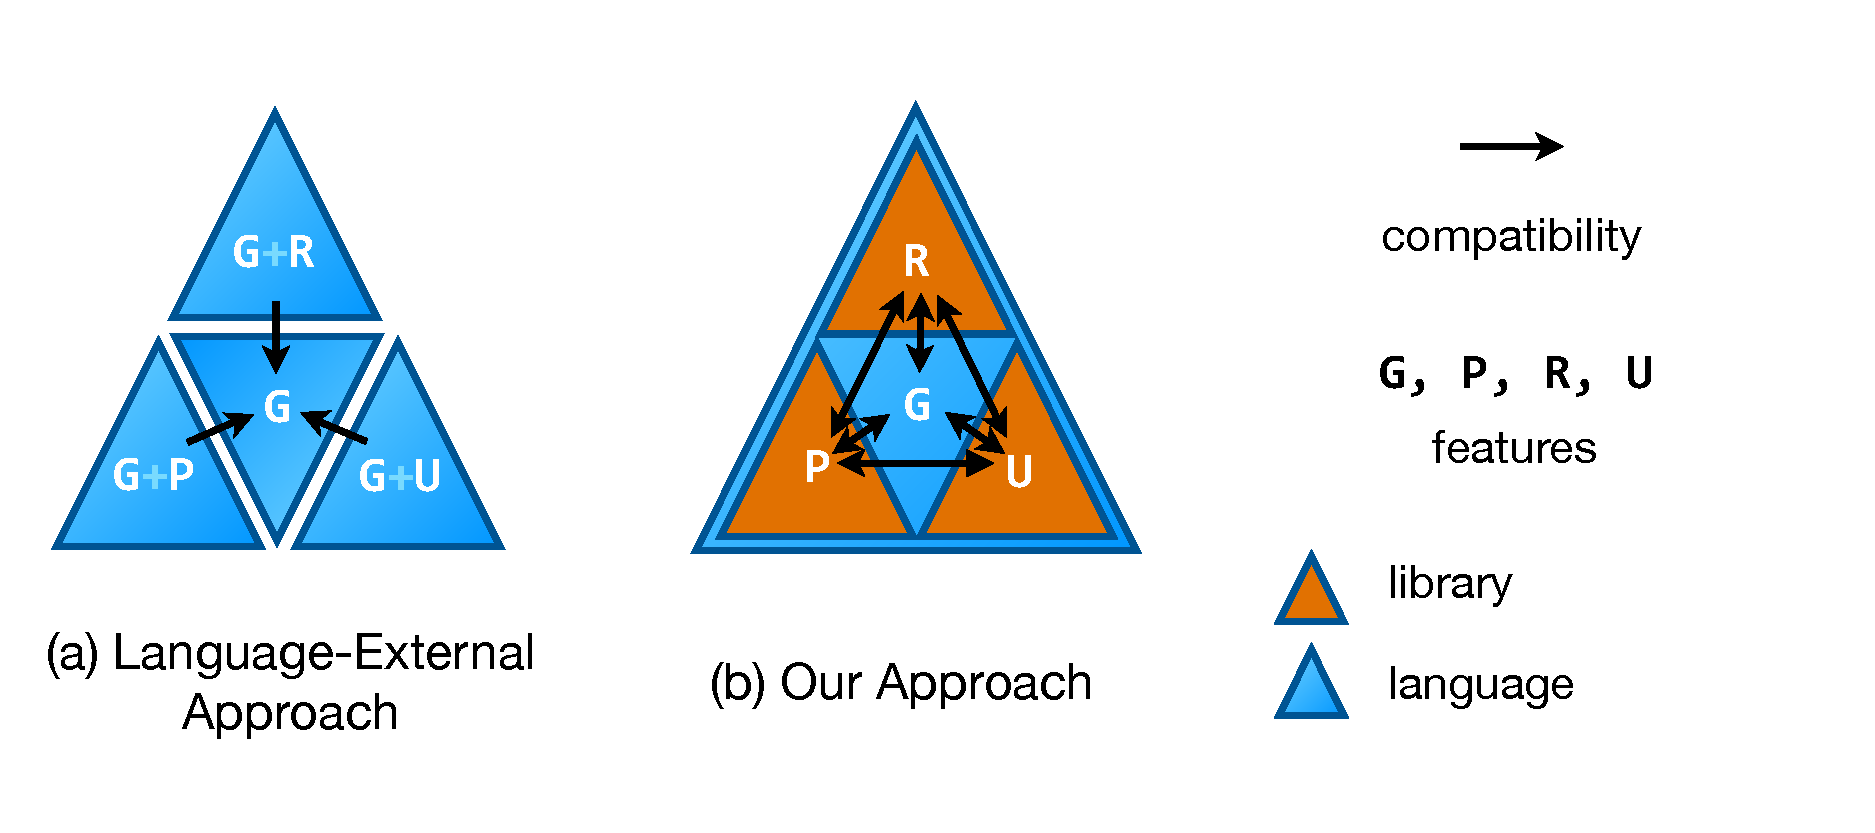
\includegraphics[scale=0.5]{approaches.pdf}
%\end{center}
%\vspace{-20px}
%\caption{\small (a) With a language-oriented approach, novel constructs are packaged into separate languages. Users can only safely and naturally call into languages consisting of common constructs (often only the common target language, such as C or Java bytecode). (b) With a language-internal extensibility approach, there is one system providing a common internal language, where additional primitive constructs that strictly strengthen its static guarantees or perform specialized code generation are specified and distributed within libraries. \label{approaches}}
%\end{figure*}

%As a result, domain-specific languages and new general-purpose abstractions alike have experienced relatively slow adoption in practice.
%
%Porting large codebases to new languages is difficult, and the dominant programming languages innovate slowly, so programming language.
%
%More specifically, such languages are neither \emph{internally extensible} because the language itself exposes only natural numbers and functions to its users, nor are they \emph{externally extensible} because no new behaviors can be added to the language's  implementation in a separate module from the one containing the initial implementation.

%This is the essence of a monolithic language implementation: it is impossible for anyone to modularly extend languages defined in this way. 

%\subsection{Theory}\label{atlam}
%%\begin{figure}
%%\begin{mathpar}
%%\inferrule{a}{b}
%%\end{mathpar}
%%\end{figure}
%In this section, we will describe a minimal calculus that captures our language-internal extensibility mechanism,  called \emph{active typechecking and translation (AT\&T)}. AT\&T allows developers to declare new primitive type families, associate operators with them, implement their static semantics in a functional style, and realize their dynamic semantics by simultaneously implementing a translation into a typed internal language. Note that this latter mechanism is closely related to how Standard ML was (re-)specified\todo{cite/read a bit about this/ask Bob/flesh this out}, but that we are fundamentally interested in extending language \emph{implementations}, not their  declarative specifications; proving the adequacy of such implementations against mechanized specifications, or extracting them directly from such specifications, will be investigated in future work.
%
%The AT\&T mechanism utilizes type-level computation of higher kind and integrates typed compilation techniques into the language to allow us to give strong metatheoretic guarantees,  and uses a mechanism notionally related to abstract types (such as those found in the ML module system) to guarantee that extensions cannot interfere with one another,  while remaining straightforward and expressive. In this section, we will develop a core calculus, called \atlam, which uses a minimal, uniform grammar for primitive operators. Then in Section \ref{ace}, we will show how to realize this minimal mechanism within a widely-used language with a more expressive grammar.
%
%AT\&T is general with respect to many choices about the type-level language, the typed internal language and syntax. Choices along these dimensions can affect both expressiveness and ease-of-use. We will begin in Sec. 2 by introducing a minimal system called $@\lambda$ (the ``actively-typed lambda calculus'') that distills the essence of the mechanism in a simply-typed, simply-kinded setting. This will allow us to fully and concisely formalize the language and compiler and give several key safety theorems. We will then continue in Sec. 3 by discussing variants of this mechanism based on other basic paradigms, considering dependently-typed functional languages and object-oriented languages, discussing trade-offs between expressivity and safety when doing so. We have developed a simple prototype called Ace and have used it to develop a number of full-scale language extensions as libraries. We will briefly discuss this language and these extensions in Sec. 4.

%We note at the outset that AT\&T focuses on extending the static semantics of languages with fixed, though flexible, syntax. Language-internal syntax extension mechanisms have been developed in the past (e.g. SugarJ \cite{sugarj}) but they have also suffered from safety problems because grammar composition is not always safe when done in an  unconstrained manner. Tyconstrained approaches that provide stronger safety guarantees have recently been outlined (e.g. Wyvern \cite{globaldsl13}) but we will leave integration of syntax extensions with semantic extensions as future work.


%\subsubsection{@$\lambda$: Conservatively Extending a Type System From Within}
\begin{figure}[t]
\small
$$\begin{array}{rccl}	
\textbf{programs} & \rho & ::= & \pfam{\familyDf}{\progsort} 
%\pipe \pdef{t}{\kappa}{\tau}{\progsort} 
\pipe e\\
		&	\theta	&	::= &	\tops{op}{\kappaidx}{i}{a}{\taut{def}} \pipe 
												\topp{\theta}{\theta}\\
\\
\textbf{external terms} 				&	e	&	::=	&	\evar{x} \pipe 
%														\efix{x}{\tau}{e} \pipe 
														\elam{\evar{x}}{\tau}{e} \pipe 
														\eop{Tycon}{op}{
															\tauidx
														}{
  												    		\splat{e}{1}{n}
														} \\
									& 		&		& 	\\


\textbf{internal terms} 				& 	\iota	&	::=	&	\evar{x} \pipe 
												\ifix{\evar{x}}{\sigma}{\iota} \pipe
												\ilam{\evar{x}}{\sigma}{\iota} \pipe 
												\iapp{\iota_{1}}{\iota_{2}} \pipe
												\iintlit \pipe \iop{\iota_{1}}{\iota_{2}} \pipe \iIfEq{\iota_{1}}{\iota_{2}}{\dint}{\iota_{3}}{\iota_{4}} \\
										& & \pipe & 
												\iunit \pipe
												\ipair{\iota_{1}}{\iota_{2}} \pipe 
												\ifst{\iota} \pipe
												\isnd{\iota} \pipe
												 \iinl{\sigma_2}{\iota_1} \pipe \iinr{\sigma_1}{\iota_2} \pipe \icase{e}{x}{e_1}{x}{e_2} \\
												
%\text{deabstracted}& \iota & ::= & \mathcal{G}[\iota, \sigma]\\
\textbf{internal types}			&	\sigma	&	::=	&    \darrow{\sigma_1}{\sigma_2} \pipe \dint \pipe \dunit \pipe \dpair{\sigma_1}{\sigma_2} \pipe \dsum{\sigma_1}{\sigma_2}  
												
\\
\\
							
\hspace{-5pt}\textbf{type-level terms} 	& \tau 	& ::= 	& 	\tvar{t} \pipe 
														\tlam{t}{\kappa}{\tau} \pipe 
														\tapp{\tau_1}{\tau_2} \pipe
														\tnil{\kappa} \pipe \tcons{\tau_1}{\tau_2} \pipe 
									                     \tfold{\tau_1}{\tau_2}{h}{t}{r}{\tau_3}
														\\
												
	 			& 		& \pipe	& 	 \iintlit \pipe \iop{\tau_1}{\tau_2} \pipe \tlabel{label} \pipe \tunit \pipe 
														\tpair{\tau_{1}}{\tau_{2}} \pipe 
														\tfst{\tau} \pipe 
														\tsnd{\tau} 
														\\	
									&       & \pipe & \tinl{\kappa_2}{\tau_1} \pipe \tinr{\kappa_1}{\tau_2} \pipe \tsumcase{\tau}{x}{\tau_1}{x}{\tau_2} \\
\text{equality}  & & \pipe & 					\tifeq{\tau_{1}}{\tau_{2}}{\kappa}{\tau_{3}}{\tau_{4}} 
														\\													\text{types} 						& 		& \pipe	& 	\ttypestd \pipe \tfamcase{\tau}{Tycon}{x}{\tau_1}{\tau_2}\\
						%				& & \pipe & \tfamcase{\tau}{Fam}{x}{\tau_1}{\tau_2}\\
																								
\text{derivates} 				& 		 & 	\pipe	&	\tden{\tauiterm}{\tautype}  \pipe \tderbind{x}{t}{\tau}{\tau_1}\\% \tdencase{\tau}{x}{t}{\tau_1}{\tau_2}\\
 %& & \pipe & 
%														\tdencase{\tau}{y}{x}{\tau_1}{\tau_2}
%														 \\

\text{reified IL}		&		&	\pipe	&	\titerm{\bar \iota} \pipe \titype{\bar \sigma} \\
% &  & \pipe & \tvalof{\tau_1}{\tau_2} \pipe \iup{\tau} \\
% 												\trepof{\tau} \pipe \dup{\tau}\\
	& \bar{\iota} & ::= & x \pipe \ifix{x}{\bar \sigma}{\bar \iota} 
	%\pipe \ilam{x}{\bar \sigma}{\bar \iota} \pipe \iapp{\bar \iota_1}{\bar \iota_2} 
	\pipe \cdots \pipe \iup{\tau} \pipe \tvalof{\tauiterm}{\tautype} \\						
 & \bar{\sigma} & ::= & \darrow{\bar \sigma_1}{\bar \sigma_2} \pipe \cdots \pipe \dup{\tau} \pipe \trepof{\tau} \\
											\\
\textbf{kinds} 					& \kappa	&	::=	&	\karrow{\kappa_1}{\kappa_2} \pipe \klist{\kappa} \pipe \kint \pipe
											    \klabel \pipe
												\kunit \pipe 
												\kpair{\kappa_{1}}{\kappa_{2}} \pipe 
												\ksum{\kappa_1}{\kappa_2} \pipe
												\kTypeBlur \pipe \kDen \pipe 
												\kITerm \pipe \kIType
												\\
\\												
%\textbf{ops signature}			& \Theta	&	::=	&	\kOpEmpty \pipe \kOp{\Theta}{op}{\kappai}\\
%											 							&		&		&	\\
\end{array}$$
\vspace{-10pt}
\caption{\small Syntax of Core \atlam. Here, $x$ ranges over external and internal language variables, $\tvar{t}$ ranges over type-level variables, $\fvar{Tycon}$ ranges over type constructor names, $\opvar{op}$ ranges over operator constructor names, $\iintlit$ ranges over integer literals, $\tlabel{label}$ ranges over label literals (see text) and $\oplus$ ranges over the standard total binary operations over integers (e.g. addition). The form $\tvalof{\tauiterm}{\tautype}$ is  used internally by the semantics (it need not be supported by a parser).%The productions related to the internal language are written using generators $\mathcal{G}$ and $\mathcal{S}$ to avoid duplicating the syntax of common terms.
\vspace{-10pt}
\label{grammar}}
\end{figure}
%\begin{figure}[t]
%\small
%\begin{flalign}
%\label{natfam}&\family{Nat}{\kunit}{\\
%\label{z}&\quad\tops{z}{\kunit}{i}{a}{\tlam{idx}{\kunit}{\tlam{args}{\klist{\kDen}}{
%	\tapp{\tapp{\tvar{if\_empty}}{\tvar{args}}}{
%		\tden{\titerm{0}}{\ttype{Nat}{\tunit}}
%	}}}};\\
%\label{s}&\quad\tops{s}{\kunit}{i}{a}{\tlam{idx}{\kunit}{\tlam{args}{\klist{\kDen}}{\\
%& \quad\quad
%	\tapp{
%		\tapp{\tvar{pop\_final}}{\tvar{args}}}{\tlam{x}{\kITerm}{\tlam{t}{\kTypeBlur}{
%			\\
%			&\quad\quad\tapp{\tapp{\tapp{\tvar{check\_type}}{\tvar{t}}}{\ttype{Nat}{\tunit}}}{
%				\tden{\titerm{\iup{\tvar{x}}+1}}{\ttype{Nat}{\tunit}}
%			}
%		}}
%		}
%	}}};\\
%\label{rec}&\quad\tops{rec}{\kunit}{i}{args}{\tlam{idx}{\kunit}{\tlam{args}{\klist{\kDen}}{\\
%& \quad\quad
%	\tapp{\tapp{\tvar{pop}}{\tvar{args}}}{\tlam{x1}{\kITerm}{\tlam{t1}{\kTypeBlur}{\tlam{args}{\klist{\kDen}}{\\
%	&\quad\quad\tapp{\tapp{\tvar{pop}}{\tvar{args}}}{\tlam{x2}{\kITerm}{\tlam{t2}{\kTypeBlur}{\tlam{args}{\klist{\kDen}}{\\
%	&\quad\quad \tapp{\tapp{\tvar{pop\_final}}{\tvar{args}}}{\tlam{x3}{\kITerm}{\tlam{t3}{\kTypeBlur}{\\
%	&\quad\quad \tapp{\tapp{\tapp{\tvar{check\_type}}{\tvar{t1}}}{\ttype{Nat}{\tunit}}}{(\\
%	&\quad\quad \tapp{\tapp{\tapp{\tvar{check\_type}}{\tvar{t3}}}{\ttype{Arrow}{(\ttype{Nat}{\tunit},\ttype{Arrow}{(\tvar{t2},\tvar{t2})})}}}{\\
%		\label{fix}&\quad\quad \tden{\titerm{\iapp{(\ifix{f}{\darrow{\dint}{\trepof{\tvar{t2}}}}{\ilam{x}{\dint}{\\
%		\label{lastop}&\quad\quad\quad \iIfEq{x}{0}{\dint}{\iup{\tvar{x2}}}{\iapp{\iapp{\iup{\tvar{x3}}}{(x-1)}}{(\iapp{f}{(x-1)})}}}})}{\iup{\tvar{x1}}}}}{\tvar{t2}}
%	)}}
%	}}}}}}}}}}}}}}
%\\
%&}{XXX}{i}{\tlam{idx}{\kunit}{\titype{\dint}}};\\
%\label{nattype}&\etdef{nat}{\kTypeBlur}{\ttype{Nat}{\tunit}}{\\
%& \elet{plus}{\ttype{Arrow}{(\tvar{nat}, \ttype{Arrow}{(\tvar{nat}, \tvar{nat})})}}{
%	\elam{x}{\tvar{nat}}{
%		\elam{y}{\tvar{nat}}{
%			\\&\quad \eop{Nat}{rec}{\tunit}{x; y; \elam{p}{\tvar{nat}}{\elam{r}{\tvar{nat}}{
%				\eop{Nat}{s}{\tunit}{r}
%			}}}
%		}
%	}
%}{\\
%& \elet{two}{\tvar{nat}}{\eop{Nat}{s}{\tunit}{\eop{Nat}{s}{\tunit}{\eop{Nat}{z}{\tunit}{}}}}{\\
%& \eop{Arrow}{ap}{\tunit}{plus; \eop{Arrow}{ap}{\tunit}{two; two}}
%}}}
%%{\\&\elet{two}{\tvar{nat}}{\eop{Nat}{s}{\tunit}{\eop{Nat}{s}{\tunit}{\eop{Nat}{z}{\tunit}{ }}}}{\eapp{\eapp{plus}{two}}{two}}}
%%}
%%\elam{x}{\tvar{nat}}{\elam{y}{\tvar{nat}}{\\
%	%&\quad \eop{Nat}{rec}{\tunit}{x; y; \elam{p}{\tvar{nat}}{\elam{r}{\tvar{nat}}{
%	%\eop{Nat}{s}{\tunit}{r}
%	%}}}}
%\end{flalign}
%\vspace{-15px}
%\caption{\small G\"odel's $\mathbf{T}$ in \atlam, used to calculate 2+2. The simple helper functions $\tvar{if\_empty}$, $\tvar{pop}$, $\tvar{pop\_final}$, $\tvar{check\_type}$ all have return kind $\ksum{\kDen}{\kunit}$ (see text). Their definitions can be found in the appendix. We use \textsf{let} to bind both external and type-level variables for clarity of presentation; these can be eliminated by manually performing the indicated substitutions (or added to the semantics).}
%\label{nat}
%\end{figure}
%
%\begin{figure}[t]
%\begin{lstlisting}
%tycon Nat of 1 with  
%    schema $\lambda$idx:1.$\blacktriangledown$($\mathbb{Z}$) 
%    opcon Z of 1 ($\lambda$idx:1.$\lambda$args:list[Elab].is_empty args $\llbracket$$\triangledown$(0) as Nat[()]$\rrbracket$)
%    opcon S of 1 ($\lambda$idx:1.$\lambda$args:list[Elab].pop_final args $\lambda$x:ITm.$\lambda$ty:$\star$. 
%      checktype ty Nat[()] $\llbracket$$\triangledown$($\vartriangle$(x)+1) as Nat[()]$\rrbracket$)
%    opcon Rec of 1 ($\lambda$idx:1.$\lambda$args:list[Elab].
%      pop args $\lambda$x1:ITm.$\lambda$ty1:$\star$.$\lambda$args':list[Elab].
%      pop args' $\lambda$x2:ITm.$\lambda$ty2:$\star$.$\lambda$args'':list[Elab].
%      pop_final args'' $\lambda$x3:ITm.$\lambda$ty3:$\star$.
%      check_type t1 Nat[()] (
%      check_type t3 Arrow[(Nat[()], Arrow[(t2, t2)])] 
%      	$\llbracket$$\triangledown$((fix f:$\mathbb{Z} \rightarrow$ rep(t2) is $\lambda$x:$\mathbb{Z}$.
%	        if x = 0 then $\vartriangle$(x2) else $\vartriangle$(x3) (x - 1) (f (x - 1))) $\vartriangle$(x1)) as t2$\rrbracket$))
%end
%\end{lstlisting}
%\caption{An implementation of primitive natural numbers as internal integers in @$\lambda$.}
%\label{nat-atlam}
%\end{figure}
In this section, we will develop an ``actively typed'' version of the simply-typed lambda calculus with simply-kinded type-level computation called @$\lambda$. More specifically, the level of types, $\tau$, will itself form a simply-typed lambda calculus. \emph{Kinds} classify type-level terms in the same way that types conventionally classify expressions. Types become just one kind  of type-level value (which we will write $\kTypeBlur$, though it is also variously written $\star$, \verb|T| and \verb|Type| in various settings). Rather than there being a fixed set of type constructors, we allow the programmer to declare new type  constructors, and give the static and dynamic semantics of their associated operators, by writing type-level functions. In the semantics for this calculus, our kind system combined with techniques borrowed from the typed compilation literature and a form of type abstraction allow us to prove strong type safety, decidability and conservativity theorems.

The syntax of @$\lambda$ is given in Fig. \ref{grammar}. An example of a program containing an extension that implements the static and dynamic semantics of G\"odel's \textbf{T} is given in Fig. \ref{nat}. We do not, of course, deny that natural numbers can be strongly encoded with a similar usage and asymptotic performance profile (but with potentially relevant additional function call overhead) by existing means (e.g. by an abstract type). We will provide more sophisticated examples where this is not the case below. %It consists of:
%a type constructor declaration, $\fvar{Nat}$, indexed trivially, together with three operator constructors, also all indexed trivially, that implement the standard introductory forms for natural numbers as well as the recursor operator (as in G\"odel's T \cite{pfpl}). Following the type constructor declaration, we apply $\fvar{Nat}$ with the trivial index, $\tunit$, to form the type $\tvar{nat}$. Finally, we write an external term that uses the operators associated with $\fvar{nat}$ and the built-in constructor $\fvar{Parr}$, governing partial functions, to define an addition function and compute the addition of the natural numbers  two and two. We will introduce a more convenient concrete syntax in later portions of this thesis; for now we will restrict ourselves to the abstract syntax so that this example can directly aid in understanding the semantics.

\subsection{Programs}

A program, $\rho$, consists of a series of static declarations followed by an external term, $e$. The syntax for external terms contains three core forms: variables, functions, and a form for all other operator invocations, which we will discuss below. Compiling a program consists of first \emph{kind checking} its static declarations and type-level terms then \emph{type checking} the external term and, simultaneously, \emph{translating} it to a term, $\iota$, in a \emph{typed internal language}. In our calculus, the internal language contains partial functions (via the generic fixpoint operator of Plotkin's PCF \cite{PCF}), simple product and sum types and a base type of integers (to make our example interesting and give a nod to practicality on contemporary machines). In practice, the internal language could be any intermediate language for which type safety and decidability of typechecking are known, as @$\lambda$ requires these to establish the corresponding theorems about the language as a whole.

The \emph{active typing judgement} relates an external term to a \emph{type} and an internal term, called its \emph{translation}, under \emph{typing context} $\Gamma$ and \emph{constructor context} $\Phi$: 
$$\ecompilesX{e}{\tau}{\iota}$$ 

This judgement follows standard conventions for the typing judgement of a simply-typed lambda calculus in most respects. The typing context $\Gamma$ maps variables to types and obeys standard structural properties. The key novelties here are that the available type and operator constructors are not fixed by the language, but rather are tracked by the constructor context, $\fvalCtx$, and that a translation is simultaneously derived. The dynamic semantics of external terms are defined by their translation to the internal language. For this judgement, the two contexts and the external term can be thought of as input, while the type and translation are output (we do not consider a bidirectional approach in this work, though this may be a promising avenue for future research).

\subsection{Types}
User-defined type constructors are declared at the top-level of a program (or package, in a practical implementation) using \textsf{tycon}. Each type constructor in the program must have a unique name, written e.g. \fvar{Nat}. We do not intrinsically consider the issue of namespacing, under the assumption that globally unique names can be generated by some extrinsic mechanism (e.g. a URI-based scheme). A type constructor must also declare an \emph{index kind}, $\kappaidx$. Types themselves are type-level values of kind $\kTypeBlur$ and are introduced by applying a previously declared type constructor to a type-level term of its index kind, $\ttype{Tycon}{\tauidx}$. The kind $\kTypeBlur$ also has an elimination form: a type can be case analyzed against a type constructor in scope to extract its index. Like open datatypes, there is no longer a notion of exhaustiveness. To maintain totality, we require the default case.

To permit the implementation of interesting type systems, the type-level language includes several other kinds of data alongside types. We lift several  standard functional constructs to the type level: unit ($\kunit$), binary sums ($\ksum{\kappa_1}{\kappa_2}$), binary products ($\kpair{\kappa_1}{\kappa_2}$), lists ($\klist{\kappa}$) and integers ($\dint$). We also include labels ($\klabel$), written in a slanted font, e.g. $\tlabel{myLabel}$, which are atomic string-like values that can only be compared, here only for equality, and play a distinguished role in the expanded syntax, as we will later discuss. Our first example, $\fvar{Nat}$, is indexed trivially, i.e. by unit kind, $\kunit$, because there is only one natural number type, $\ttype{Nat}{\tunit}$, but we will show examples of type constructors that are indexed in more interesting ways in later portions of this work. For example, $\fvar{Tuple}$ is indexed by a list of types and $\fvar{LabeledTuple}$ is indexed by a list pairing labels with types.  

Two type-level terms of kind $\kTypeBlur$ are equivalent if they apply the same constructor, identified by name, to equivalent indices. Going further, we ensure that deciding type equivalence requires only checking for syntactic equality after evaluation to normal form by imposing the restriction that type constructors can only be indexed by kinds for which equivalence can be decided in this way. All combinations of kinds introduced thus far  have this property and this is sufficient for many interesting examples. We leave  introducing a richer notion of  equivalence of types that  extension providers can extend as future work, as the metatheoretic guarantee that typing respects type equivalence would be quite a bit more complex in such a setting.% (a na\"ive approach to this would impose non-trivial extrinsic proof obligations onto extension developers that, unlike in others in this thesis, could threaten type safety).

Type constructors are not first-class; they do not themselves have arrow kind as in some kind systems (e.g.  \cite{Watkins08}\todo{cite}; Ch. 22 of \emph{PFPL} describes a related system \cite{pfpl}). The type-level language does, however, include total functions of conventional arrow kind, $\karrow{\kappa_1}{\kappa_2}$. Type constructor application can be wrapped in a type-level function to emulate first-class type constructors (and indeed, such a wrapper could be generated automatically, though we avoid this for simplicity in our semantics). Equivalence at arrow kind does not coincide with $\beta$-equivalence, so type-level functions cannot appear in type indices. Our treatment of equivalence in the type-level language is thus quite similar to the treatment of term-level equality using ``equality types'' in a language like Standard ML. Indeed, one might imagine that a practical implementation of our calculus would start with a pure, total subset of the term language of ML to construct the type-level language (consistent with its early development as a ``metalanguage'' and, as we will see, the role of our type-level language as a DSL for implementing type systems and translators, which functional languages are widely considered well-suited for as-is). We leave the development of such an implementation (and of bootstrapping type-level and internal languages that are themselves user-defined or extensible) as areas for future work.
\subsection{Operators}
User-defined operator constructors are declared using \textsf{opcon}. For reasons that we will discuss, our calculus associates every operator constructor with a type constructor. The \emph{fully-qualified name} of the operator constructor, e.g. $\fvar{Nat}.\opvar{z}$, must be unique. Operator constructors are indexed by type-level values, like type constructors, and so also declare an index kind $\kappaidx$. In our first example, all the operator constructors are indexed trivially, but later examples will use more interesting indices. For example, the projection operators for tuples and labeled tuples use numbers and labels as indices, respectively.
Note that neither operator constructors nor operators are first-class type-level values (we plan to investigate  lifting the latter restriction) and we do not impose any restrictions on their index kinds.

In the external language, an operator is selected and invoked by applying an operator constructor to a type-level index and $n \geq 0$ \emph{arguments}, $\eop{Tycon}{op}{\tauidx}{\splat{e}{1}{n}}$. For example, on line 18 of Fig. \ref{nat}, we see the operator constructors $\fvar{Nat}.\opvar{z}$ and $\fvar{Nat}.\opvar{s}$ being invoked to compute two.\footnote{Although our focus here is entirely on semantics, a brief note on syntax: in the expanded syntax, the trivial indices and empty argument lists can be omitted, so we could write \texttt{Nat.s(Nat.s(Nat.z))}. With the ability to ``open'' a type's operators into the context, we could shorten this still to \texttt{s(s(z))}. Alternatively, with the ability to define a TSL in a manner similar to that in Sec. \ref{aparsing}, we might instead just write \texttt{2}.}
To derive the active typing judgement for this form, the semantics invokes  
 the operator constructor's  \emph{definition}: a type-level function that must examine the provided operator index and the recursively determined \emph{derivates} of the arguments to determine a derivate for the operation as a whole,  or indicate an error. A derivate is a type-level representation of the result of deriving the active typing judgement\footnote{Technically, the abstract active typing judgement, which is similar in form and we will introduce shortly.}: an internal term, called the {translation},  paired with a type. Derivates have kind $\kDen$ and introductory form $\tden{\tautrans}{\tautype}$. The elimination form $\tderbind{x}{t}{\tau}{\tau'}$ extracts the translation and type from the derivate $\tau$, binding it to $\tvar{x}$ and $\tvar{t}$ respectively in $\tau'$. 
%Indeed, one might be tempted to simply define derivates as products. However, we treat translations with much care throughout the calculus, so this is not quite the case (we will return to this shortly). 
Because constructing a derivate is not always possible (e.g. when there is a type error in the client's code, or an invalid index was provided), the return kind of the function is an ``option kind'', $\ksum{\kDen}{\kunit}$, where the trivial case indicates a statically-detected error in the client's program. In practice, it would instead require providers to report information about the precise location of the error and an appropriate error message.
 
A translation, as we have said, is an internal term. To construct an internal term using a type-level function, as we must do to construct a derivate, we must expose a type-level representation of the internal language. A \emph{quoted internal term} is a type-level value of kind $\kITerm$ with introductory form $\titerm{\bar \iota}$ and a \emph{quoted internal type} is a type-level value of kind $\kIType$ with introductory form $\titype{\bar \sigma}$. Neither kind has an elimination form. Instead, the syntax for the quoted  internal language includes complementary \emph{unquote forms} $\iup{\tau}$ and $\dup{\tau}$ that permit the interpolation of another quoted term or type, respectively, into the one being formed. Interpolation is capture-avoiding, as our semantics will clarify. We have now described all the kinds in our language.

The definition of $\fvar{Nat}.\opvar{z}$ is quite simple: it returns the derivate $\tden{\titerm{0}}{\ttype{Nat}{\tunit}}$ if no arguments were provided, and indicates an error (an \emph{arity error}, though we do not distinguish this in our calculus) otherwise. This is done by calling a simple helper function, $\tvar{is\_empty} : \karrow{\klist{\kDen}}{\karrow{\kDen}{(\ksum{\kDen}{\kunit})}}$, that selects the appropriate case of the sum given the derivate that should be produced if the list is indeed empty. The definition of $\fvar{Nat}.\opvar{s}$ is only slightly more complex, because it requires inspecting a single argument. The helper function $\tvar{pop\_final} : \karrow{\karrow{\klist{\kDen}}{(\karrow{\kTypeBlur}{\karrow{\kITerm}{(\ksum{\kDen}{\kunit})})}}}{(\ksum{\kDen}{\kunit})}$ ``pops'' a derivate from the head of the list and, if no other arguments remain, passes its translation and type to the ``continuation'', returning the error case otherwise. The continuation checks if the argument type is equal to $\ttype{Nat}{\tunit}$ using $\tvar{check\_type} : \karrow{\kTypeBlur}{\karrow{\kTypeBlur}{\karrow{\kDen}{(\ksum{\kDen}{\kunit})}}}$, which operates similarly. If these arity and type checks succeed, the resulting derivate is composed by adding one to the translation of the argument, passed into the continuation as $\tvar{x}$ in our example, and pairing it with the natural number type: $\tden{\titerm{\iup{\tvar{x}} + 1}}{\ttype{Nat}{\tunit}}$. We will return to the definition of $\fvar{Nat}.\opvar{rec}$ after in the next subsection.

By writing the typechecking and translation logic in this way, as a total function, we are taking a rather ``implementation-focused view'' rather than attempting to extract such a function from a declarative specification. That is,  we leave to the provider (or to a program generator or kind-specific language that transforms such a specification into an operator definition) the problem of finding a deterministic algorithm that adequately implements their intended semantics, allowing us to prove decidability of typechecking for the language as a whole by essentially just citing the termination theorem for the type-level language. We also avoid difficulties with error reporting in practice. Rob Simmons' undergraduate thesis has a good discussion of these issues \cite{rjs-princeton}.

Because the input to an operator definition is the recursively determined derivate of the argument in the same context as the operator appears in, our mechanism does not presently permit the definition of operator constructors that bind variables themselves or require a different form of typing judgement (e.g. additional forms of contexts). This is also why the $\lambda$ operator constructor needs to be built in. It is the only operator in our language that can be used to bind variables. The type constructor $\fvar{Arrow}$ can be defined from within the language (and is included in the ``prelude'' constructor context), but only defines the operator constructor, $\opvar{ap}$. These two operators translate to their corresponding forms in the internal language directly, as we will discuss below. We leave adding the ability to declare and manipulate new contexts as future work.

\subsection{Representational Consistency Implies Type Safety}
In our example, natural numbers are represented internally as integers. Were this not the case -- if, for example, we added an operator constructor $\fvar{Nat}.\opvar{z2}$ that produced the derivate $\tden{\titerm{\iinl{\dint}{\iunit}}}{\ttype{Nat}{\tunit}}$, then there would be two different internal types, $\dint$ and $\dsum{\dunit}{\dint}$,  associated with a single external type, $\ttype{Nat}{\tunit}$. This makes it impossible to operate compositionally on the translation of an external term of type $\ttype{Nat}{\tunit}$, so our implementation of $\fvar{Nat}.\opvar{s}$ would produce ill-typed translations in some cases but not others. Similarly, we wouldn't be able to write functions over all natural numbers because there would not be a well-typed translation to give to such a function.

To reason compositionally about the semantics of well-typed external terms when they are given meaning by translation to a typed internal language, we must have the following property: for every  type, $\tau$, there must exist an internal type, $\sigma$, called its \emph{representation type}, such that the translation of every external term of type $\tau$ has internal type $\sigma$. This principle of \emph{representational consistency} arises essentially as a strengthening of the inductive hypothesis necessary to prove that all well-typed external terms translate to well-typed internal terms, precisely because operators like $\lambda$ and $\fvar{Nat}.\opvar{s}$ are defined compositionally. It is closely related to the concept of \emph{type-preserving compilation} developed by Morrisett et al. for the TIL compiler for Standard ML \cite{TIL}\todo{cite}. %That is, instead of being used as a necessary condition for compiler correctness, we are using it as a sufficient condition for type safety. 
%We emphasize the distinction between translation (which in our calculus endows terms with a dynamic semantics) and compilation (which must preserve the dynamic semantics of terms). %In the presence of extensions, checking for representational consistency becomes subtle if we wish to guarantee conservativity, as we will discuss in the next subsection.

It is easy to show by induction that, under a ``closed-world assumption'' where the only available operators are $\fvar{Nat}.\opvar{z}$ and $\fvar{Nat}.\opvar{s}$, the representation type of $\ttype{Nat}{\tunit}$ is $\dint$. If we can maintain this under an ``open-world assumption'' (requiring that, for example, applications of operator constructors like $\fvar{Nat}.\opvar{z2}$, above, are not well-typed), and we target a type safe internal language, then we will achieve type safety: well-typed external terms cannot go wrong, because they always translate to well-typed internal terms, which cannot go wrong. For the semantics to ensure that representational consistency is maintained by all operator definitions, we require that each type constructor must declare a \emph{representation schema} with the keyword \textsf{schema}. This must be a type-level function of kind $\karrow{\kappaidx}{\kIType}$, where $\kappaidx$ is the index kind of the type constructor. When the compiler needs to determine the representation type of the type $\ttype{Tycon}{\tauidx}$ it simply applies the representation schema of $\fvar{Tycon}$ to ${\tauidx}$.

As described above, the kind $\kIType$ has introductory form $\titype{\bar \sigma}$ and no elimination form. There are two forms in $\bar \sigma$ that do not correspond to forms in $\sigma$ that allow quoted internal types to be formed compositionally:
\begin{enumerate}
\item $\dup{\tau}$, already described, unquotes (or ``interpolates'') the quoted internal type $\tau$
\item $\trepof{\tau}$ refers to the representation type of type $\tau$ (we will see in the next subsection why this needs to be in the syntax for $\bar \sigma$ and not directly in the type-level language)
\end{enumerate}

These additional forms are not needed by the representation schema of $\fvar{Nat}$  because it is trivially indexed. In Fig. \ref{tuple}, we show an example of the type constructor $\fvar{Tuple}$, implementing the semantics of $n$-tuples by translation to nested binary products. Here, the representation schema requires referring to the representations of the tuple's constituent types, given in the type index\todo{add this example from appendix of ESOP}.

Operator constructor definitions might also need to refer to the representation of a type. We see this in the definition of the recursor on natural numbers, $\fvar{Nat}.\opvar{rec}$. After checking the arity and extracting the types and translations of its three arguments, it produces a derivate that implements the necessarily recursive dynamic semantics using a fixpoint computation in the internal language. This fixpoint computation produces a result of some arbitrary type, $\tvar{t2}$. We cannot know what the representation type of $\tvar{t2}$ is, we refer to it abstractly using $\trepof{\tvar{t2}}$. The translation is well-typed no matter what the representation type is. In other words, a proof of representational consistency of the derivate produced by the definition of $\fvar{Nat}.\opvar{rec}$ is parametric (in the metamathematics) over the representation type of $\tvar{t2}$. This leads us into the concept of conservativity.

\subsection{Parametricity Implies Conservativity}
In isolation, our definition of natural numbers can be shown to be a strong encoding of the semantics of G\"odel's $\mathbf{T}$. That is, there is a bijection between the terms and types of the two languages and the typing judgements preserve this mapping. Moreover, we can show by a bisimulation argument that the translation produced by @$\lambda$ implements the dynamic semantics of G\"odel's $\mathbf{T}$. We will provide more details on this later. A necessary lemma in the proof, however, is that the value of every translation of an external term of type $\ttype{Nat}{\tunit}$ is a non-negative integer. This is needed to show that the fixpoint computation in the definition of $\fvar{Nat}.\opvar{rec}$ is terminating, as the recursor always does in $\mathbf{T}$. A very similar lemma is needed to show that the translation of every external term of type $\ttype{Nat}{\tunit}$ is equivalent to the translation that would be produced by some combination of applications of $\fvar{Nat}.\opvar{z}$ and $\fvar{Nat}.\opvar{s}$ (the analog to a canonical forms lemma in our setting). Fortunately, the definitions we have provided thus far admit such lemmas.

However, these theorems are all quite precarious because they rely on exhaustive induction over the available operators. As soon as we load another library into the program, these theorems may no longer be \emph{conserved}. For example, the following operator declaration in some other type that we have loaded would topple our house of cards:





%If g : nat then [[g]] : Nat[()] -> i and i : Z and there exists an i' s.t. i |->* i' and i' val and geq i' -1 |->* 1.
%
%[[z]] := Nat.z[()]()
%[[s(e)]] := Nat.s[()]([[e]])
%If |- e' : t then [[rec(e; e'; x.y.e'')]] := Nat.rec[()]([[e]]; [[e']]; \x:Nat[()].\y:[[t]].e'')
%[[nat]] := Nat[()]
%[[t -> t']] := Arrow[([[t]], [[t']])]
%[[x]] := x
%[[\x:t.g]] := \x:[[t]].[[g]]
%[[g g']] := Arrow.ap[()]([[g]]; [[g']])
%
%If |- g : nat then g \evals g' and |- [[g]] : Nat[()] -> i
%  s.t. |- i : Z and if if i \evals i' then 
%    gt i' -1 |->* 1 and 
%    |- [[g']] : Nat[()] -> i'' s.t. 
%    if i'' \evals i''' then i' = i'''.
%    
%If |- e : Nat[()] -> i then |- [[e]] : nat and [[e]] |-> g' and |- [[g']] : Nat[()] -> i' and if i \evals i'' and i' evals i''' then i'' = i'''.
%
%The proof relies on the following lemma:
%If |- e : Nat[()] -> i then if i evals i', gt i' 0 evals 1.
%
%Without it, the case for the recursion operator, which requires fixpoint induction, would not terminate. 
%  
%g |-> g' s.t. g' val then |- [[g']] : Nat[()] -> i''
%  |- i'' : Z
%  i'' |->* i'
%
%[[Nat.z[()]()]] := z
%[[Nat.s[()](e)]] := s([[e]])
%[[Nat.rec[(()](e; e'; e'')]] := rec([[e]]; [[e']]; [[e'']])
%[[\x:tau.e]] := \x:[[tau]].[[e]]
%...
%
%If |- e : Nat[()] -> i then |- [[e]] : nat and [[e]] |-> g' and i -> i' and [[g']] : Nat[()] -> i'' s.t. i'' ->* i'.
%

%
%It can also be shown to maintain the invariant that natural numbers elaborate into \emph{non-negative} internal integers. Note that because we are beginning with a simply-typed, simply-kinded formulation, these kinds of statements must be proven metatheoretically (as with other sorts of complex invariants in simply-typed languages). With a naive formulation of this mechanism, these theorems would be quite a bit more precarious, however. If another provider, perhaps a malicious one, declares a new operator constructor that introduces natural numbers, these theorems may not be \emph{conserved}. For example, the following operator declaration is quite problematic

\todo{In progress below}:

\begin{lstlisting}
opcon badnat of 1 ($\lambda$idx:1.$\lambda$args:list[Elab].$\llbracket\triangledown$(-1) as Nat[()]$\rrbracket$)
\end{lstlisting}

With this declaration, there is now a new and unexpected introductory form for the natural number type, and even worse, it violates our previous implementation invariants. A naive check for type preservation would not catch this problem: \li{-1} does have type $\mathbb{Z}$, it is simply not an integer that could have been emitted by the original definition of \li{Nat}.

To prevent this problem, we \emph{hold the representation of a type abstract} outside of the operators explicitly associated with it. If \li{badnat} cannot know that the representation of \li{Nat[()]} is $\mathbb{Z}$, then the above operator implementation cannot be correct. Because we cannot prove relational correctness properties from within a simply-typed/kinded calculus, our semantics enforces this by using a form of value abstraction, similar to that described by Zdancewic et. al \cite{zdancewic}. In brief: the representation of a type, written $\trepof{\tautype}$, does not reduce further to the actual representation type (e.g. to $\mathbb{Z}$) when not in an operator definition associated with $\tautype$. The only internal form that can be checked against  $\trepof{\tautype}$ is the special form $\tvalof{\tauiterm}{\tautype}$, an abstracted internal term corresponding to the internal term reflected by $\tauiterm$. Rather than exposing it explicitly, it is wrapped so that it can't be checked against any type other than $\trepof{\tautype}$. A full description of this mechanism (and the others, described above) requires us to introduce the semantics in detail. A draft of the semantics of @$\lambda$ is available as a paper draft\footnote{\url{https://github.com/cyrus-/papers/tree/master/esop14}}.

%
%\subsection{Operators}
%As indicated, operators other than $\lambda$ and \textsf{fix} in @$\lambda$ are associated with type constructors (for reasons we will discuss), so an external term of the form $\eop{Tycon}{op}{\tauidx}{\splat{e}{1}{n}}$ applies the operator $\opvar{op}$ associated with type constructor $\fvar{Tycon}$ to operator index $\tauidx$ and zero or more arguments, written in our syntax and semantics using the shorthand ${\splat{e}{1}{n}}$ for concision. We can see on line X the application of the $\tvar{z}$ and $\tvar{s}$ constructors to form the natural number \texttt{s(s(z))}, for example:
%$$\eop{Nat}{s}{()}{\eop{Nat}{s}{()}{\eop{Nat}{z}{()}{ }}}$$
%
%Operator constructors, like type constructors, are indexed by type-level values. In our example, all the operators are indexed trivially, but we will see examples later where non-trivial operator indices are useful. For the sake of uniformity, we include trivial indices, but in a concrete syntax for such a language, these could be omitted. We will discuss why operator constructors are associated directly with type constructors, rather than existing as standalone entities, when we discuss the scoping mechanism for the representation schema. This coupling also forms the foundation for the higher-level elaboration mechanism that allows us to use more conventional and concise (though still fixed) syntactic idioms, which we intend to explore in this thesis, but have not yet formalized. For now, we simply note that intuitively, most operators are either introduction or elimination forms for a particular type, so we are simply encoding a common idiom. Free-floating operator constructors could be introduced to this calculus with little difficulty.
%
%The declarations of the three operator constructors related to natural numbers are given on lines 3-13 of Fig. \ref{nat-atlam}. Operator constructors are declared by specifying the kind of type-level value they are indexed by and giving an \emph{operator definition}, a type-level function of kind $\kappa \rightarrow \klist{\kDen} \rightarrow \kDen$. The kind $\kDen$ classifies \emph{elaborations}. There are two introductory forms for this kind: \emph{valid elaborations}, $\tden{\tauiterm}{\tautype}$, consist of a reflected internal language term paired with a type assignment, while \emph{error elaborations}, $\terr$, represent a type error (in a full implementation, the error elaboration would contain an error message, as discussed above, but for simplicity in our core calculus, we simply treat all type errors equivalently). Internal terms, $\iota$, like internal types, are reflected as type-level terms of kind $\kITerm$ via the introductory form $\titerm{\iota}$. The form $\iup{\tau}$ interpolates a type-level value of kind $\kITerm$ into an internal term.  Note that there are no elimination forms for the kinds $\kIType$ and $\kITerm$. Composition occurs entirely via interpolation -- syntax trees are never examined directly by extensions in @$\lambda$. 
%
%Operator definitions are called by the compiler to generate an elaboration for operator invocations. In our example, the definition of $\fvar{Nat}.\opvar{z}$ simply checks that there were no arguments (using a simple helper function for working with lists of elaborations, \li{is_empty}, not shown) and if so, provides an elaboration where the internal language integer \li{0} is associated with type $\ttype{Nat}{\tunit}$. If the list is not empty, \li{is_empty} simply returns $\terr$. The other two operator constructors are more verbose, but follow a similar pattern -- elaborations are popped off and broken down into their constituent internal terms and types by helper functions, then a functional program that implements the intended semantics is written to produce an elaboration as a whole. Note that the \li{Rec} operator does not itself bind new variables; it must use the built-in \li{Arrow} type constructor. There is no support in @$\lambda$ for introducing new forms of binding; $\lambda$ is the only available binding operator. Note that application is invoked like other operators: $\eop{Arrow}{ap}{\tunit}{e_1; e_2}$.
%
%
%\subsection{Kind Checking and Normalization}
%
%\subsection{Type Checking}

%\subsubsection{Abstract Internal Typechecking}
%
%\subsubsection{Deabstraction}
%
%\subsection{Safety}
%Type safety of TL. Type safety of IL. Type preserving compilation. Type safety of EL. Strong normalization of TL. Decidability of type checking. Conservativity.
%
%
% %Kind checking  can be expressed judgementally as follows:\todo{compilation judgement}
%
%
%
%
%
%\paragraph{Type Constructors} Type constructors are indexed by A type constructor is declared by providing a name, like $\fvar{Tuple}$, an index kind, like %$\list$
%
%Note that this calculus be compared to the ``core language'' of expressions and types in a language in Standard ML; a module language similar to ML's could be layered on top of this core in a completely standard way. Note also that we do not include polymorphism and recursive types in this calculus (nor can they be defined, because we do not support type binders). This is both to simplify the calculus and because it is known that polymorphism is conservative over simple types \cite{breazu1990polymorphism} (by similar arguments, recursive types are conservative over a simply typed language with fixpoints, which we do include).
%
%The semantics of the language are in the style of the Harper-Stone elaboration semantics for Standard ML: all terms in an external language, $e$, are simultaneously assigned a type and an elaboration to a term, $\iota$, in a fixed typed internal language. The mechanism checks that any generated elaborations are \emph{type preserving} -- that all external terms of a particular type, $\tau$, elaborate to internal terms with a consistent internal type, $\sigma$ -- following the approach taken in the TIL compiler for Standard ML by Morrisett et al. \cite{TIL}. This allows the semantics to be reasoned about compositionally and, when combined with type safety of the internal language, gives us type safety of the extensible external language. 
%
%This design ensures that global properties that the internal language maintains are guaranteed to hold no matter which extensions are introduced. In other words, extension providers cannot implement type systems weaker than the type system of the internal language. Providers are, however, able to implement type systems that maintain invariants stronger than those the internal type system can maintain. The internal language of @$\lambda$ is PCF with simple products and one base type, integers. Because of the availability of the fixpoint operator, the internal language is universal (i.e. Turing-complete).
%
%It is reasonable, if we wish to actually program with such a language, to permit only the addition of deterministic, decidable rules to the semantics. Extension logic is thus implemented in a functional style  (essentially, lifting fragments of the typechecker into the type-level language), rather than extracted from inductive specifications, like those at the beginning of Sec. \ref{att}\footnote{Though we will not explore this further in this thesis, a system for extracting such a function from a declarative specification could potentially be implemented using the techniques in Sec. \ref{aparsing} -- a \emph{kind-specific language}!}. This has the added benefit of giving providers finer-grained control over error reporting. When extracting an implementation from a typical inductive specification, which only specifies ``success conditions'', it is difficult to provide different error messages at different failure points within a single rule.
%%In this section, we will sketch a calculus where new type families and operator families can be introduced by users. The type synthesis and translation logic that implements the desired static and dynamic semantics, respectively, for these is implemented in the type-level language. 
%
%To enable this, the language must allow for the introduction of new type constructors, like \verb|Tuple|, operator constructors, like \verb|NewTuple| and \verb|Prj|, and their associated static and dynamic semantics. Type and operator constructors can no longer be indexed by compiler-internal values in such a design. 
%%We are also be considering only simply-typed languages -- those with a clear phase separation between compile-time and run-time -- so we will not consider dependent types, though extensibility mechanisms for dependently typed languages are an interesting avenue of future work.\footnote{Note that types indexed by expressions are distinct from type names that have metadata expressions associated with them, as in Wyvern. Metadata does not impact type equality, for example.} 
%We will instead use type-level values. This requires supporting more kinds of values in the type-level language, conventionally written $\tau$, than just types, and thus the type-level language must have a non-trivial semantics. The ``types'' of type-level terms are called \emph{kinds} for clarity. Types simply become a particular kind of type-level value (we will call it $\star$) and are introduced uniformly by naming an available type constructor and providing an index of the kind that constructor specifies. For example, the type constructor \verb|Tuple| is indexed by type-level values of kind \verb|list[|$\star$\verb|]| so a 3-tuple type might be written \verb|Tuple[cons(nat, cons(string, cons(nat, nil)))]|. Note that we do not identify type constructors and type-level functions, as in some kind systems (\verb|Tuple| is \emph{not} itself of kind \verb|list[|$\star$\verb|] |$\rightarrow$\verb| |$\star$). One can wrap constructor application with a type-level function to achieve the same effect (and avoid an awkward canonical forms lemma and beta-reduction rules).
%
%Operator constructors are similarly indexed by type-level values. For example, the projection operator written \verb|#2| in a language like Standard ML might be written \verb|prj[2]| in our work. Here, \verb|prj| is an operator constructor indexed by a type-level natural number. 
%To define an operator, we must also provide it with a static and dynamic semantics. We will, as in our work on Wyvern and consistent with our exposition above, take an approach similar to Harper and Stone in their definition of Standard ML where the dynamic semantics of external language terms are given by translation into a  typed internal language \cite{Harper00atype-theoretic}. Operator definitions must work with types, type indices and operator indices, all of which are type-level values, so we will argue that it is sensible to give these elaborations as type-level functions (appropriately constrained, as we will show). 
%
%-----
%
%To give a first example, the code in Fig. \ref{nat-atlam} (written using concrete syntax) shows how to introduce a new type constructor, $\fvar{Nat}$, indexed trivially (i.e. by a type-level value of kind 1, also known as unit). Types themselves are type-level values of kind $\kTypeBlur$ and are introduced by naming a type constructor and providing an index of the appropriate kind: $\ttype{Nat}{\tunit}$. To ensure that type equality is decidable, type constructors can only be indexed by values of a kind for which equality is ``trivially'' decidable (i.e. where semantic equality coincides with syntactic equality). This means that types themselves, as well as type-level data structures containing values of kinds with this property, can be used, while type-level functions cannot. We leave a richer consideration of type equality to future work for now.
%
%To ensure that compilation is type-preserving, as described above, each type must have an internal type, called its \emph{representation}, associated with it. The representation of a type might depend on its index, so each type constructor must declare a type-level function, called its \emph{representation schema}, that returns an internal type given a type's index. An internal type, $\sigma$, is reflected as a type-level term of kind $\kIType$ via the introductory form $\blacktriangledown(\sigma)$. Because $\fvar{Nat}$ is indexed trivially, it simply returns the reflected form of the internal type $\mathbb{Z}$. %The sort $\sigma$ also contains forms $\trepof{\tau}$ and $\dup{\tau}$. The former allows one to refer, abstractly, to the representation of the type $\tau$, while the latter enables the interpolatation of a type-level value of kind $\kIType$.
%
%%Two additional forms, $\tvalof{\tauiterm}{\tautype}$ and $\iup{\tau}$, will be discussed below. These are erased by the end of the elaboration process.
%
%--
%

\subsection{Expressiveness}
The use cases permitted by this mechanism are not simply subsumed by a module system with support for abstract types and functors. Indeed, such a module system is an orthogonal concern in that it must sit atop a core type system. More particularly, the distinction is the fundamental one between functions and operators. Functions cannot examine type indices at compile-time to determine a return type and implementation (or generate static error messages), as operators are able to do. It is encouraging that there are clear parallels between module systems with abstract types and type constructors with abstract schemas, and any full-scale language design based on this mechanism should certainly provide both mechanisms (with the former used in most cases). We plan to investigate this relationship more thoroughly, showing examples where abstract types are more clearly unsuitable, in the remainder of this work. 


\subsubsection{Remaining Tasks and Timeline}
We are actively working on this mechanism and plan to submit a paper to ICFP 2014 on Mar. 1 based on a submission to ESOP 2014 that was not accepted. The following key tasks, other than clarifying the writing, remain to be completed:

\begin{enumerate}
\item Reviewers of the previous submission to ESOP found a problem with our treatment of internal type variables that needs to be corrected by threading a context through the type-level evaluation semantics.
\item We must more rigorously state and prove the key lemmas and theorems related to type preservation, type safety, decidability and conservativity. 
\item We must develop examples that are more interesting than natural numbers. In particular, some interesting form of labeled product type that SML doesn't have (e.g. a record with prototypic dispatch) as well as sum types would be interesting.
\item We must consider whether properties related to termination can be conserved by this mechanism, because a fixpoint can be used to introduce a non-terminating expression of any type. This may be possible by being careful about how deabstraction interacts with fixpoints.
\item We must more clearly connect this work to the Harper-Stone semantics and other related work, and clarify  the relationship to abstract types.
\item We must show how to add additional syntactic forms to the external language that defer to the generic operator invocation form in a type-directed manner. This connects the theory to the work on Ace, described below. 
\end{enumerate}

\section{Ace}\label{ace}
 Using a type-level language that provides few strictly enforced semantic guarantees makes giving strong metatheoretic guarantees about Ace more difficult. Ace does include some checks similar to those in @$\lambda$ that catch accidental problems but they can be intentionally subverted by untrusted extension providers using the dynamic metaprogramming features of Python. This is sufficient for programmers who use a type system to help catch errors. We conjecture, but do not plan to show in detail, that it would be possible to use Ace to bootstrap a statically-typed subset of Python that, if used to compile extension logic, would be sufficient to provide theoretical guarantees comparable to @$\lambda$ (building, perhaps, on recent work that resulted in a mechanized semantics for Python \cite{pysem}).

\subsection{From Extensible Compilers to Extensible Languages}\label{evolution}
The monolithic character of most programming languages is reflected in, and perhaps influenced by, the most common constructs used for implementing programming languages.
Let us consider an implementation of the STLC. 
A compiler written using a functional language will invariably represent the primitive type  and operator constructors using {closed} recursive sums. 
For example, a simple implementation in Standard ML might be based around these datatypes (where variables, binders and operator application to arguments are handled separately, not shown)\footnote{This is essentially the approach that we took in the infrastructure for the coding assignments in 15-312.}:
\begin{lstlisting}
  datatype Ty = Arrow of Ty * Ty
  datatype Op = Lam of Ty | Ap 
\end{lstlisting}

%The compiler front-end, which consists of a typechecker and translator to a suitable intermediate language,    proceeds by exhaustive case analysis over the constructors of \verb|Op|.

In a class-based object-oriented implementation of the STLC, we might instead encode type and operator constructors as subclasses of abstract classes \verb|Ty| and \verb|Op|. If typechecking and translation proceed by the common \emph{visitor pattern}, dispatching against a fixed set of {known} subclasses of \verb|Op|, then we encounter a similar issue: everything is defined at once. 

This issue was first discussed by Reynolds \cite{Reynolds75}. A number of mechanisms have since been proposed that allow new cases to be added to data types and the functions that operate over them in a modular manner. 
In functional languages, we might turn to \emph{open datatypes and open functions} \cite{conf/ppdp/LohH06}. For example, we might add a new type constructor, \verb|Tuple|, indexed by a list of types, and two new operator constructors: an introductory form, \verb|NewTuple|, indexed trivially, and an elimination form, \verb|Prj|, indexed by a natural number (hypothetical syntax):
\begin{lstlisting}
  newcon Tuple of Ty list extends Ty
  newcon NewTuple extends Op
  newcon Prj of nat extends Op
\end{lstlisting}

The logic for functionality like typechecking and translation, if organized around open functions, can then be implemented for only these new cases. For example, the \verb|optype| function that synthesizes a type for an operator invocation given a  a list of argument types might be extended to support the new constructor \verb|Prj| like so:
\begin{lstlisting}
  optype (Prj(n), [t]) = case t of 
      Tuple(ts) => (case List.nth n ts of 
          Some t' => t'
        | _ => raise IndexError("<projection index out of bounds>"))
    | _ => raise TypeError("<tuple expected>")
  optype (ctx, Prj(n), _) = raise ArityError("<expected 1 argument>")
\end{lstlisting}

Using a class-based mechanism, we might dispense with the visitor pattern and instead invert control to abstract methods of \verb|Op|. 

\begin{lstlisting}[language=Java]
class Prj extends Op {
  Prj(Nat n) { this.n = n; }
  Nat n;
  Ty optype(List<Ty> args) {
    if (args.length != 1) throw new ArityError("<expected 1 argument>")
    Ty t = args[0];
    if (t instanceof Tuple) {
      Tuple t = (Tuple) t;
      try {
        return t.idx[this.n]
      } catch OutOfBoundsException(e) {
        throw new IndexError("<projection index out of bounds>");
      }
    } else throw new TypeError("<tuple expected>");
  }
}
\end{lstlisting} 

If we allowed programmers to load definitions like these into our compiler by, e.g., a pragma declaration, we will still have only succeeded in creating an extensible compiler. We have not created an extensible programming language because other compilers for the same language will not necessarily support the same extensions. These mechanisms are not truly \emph{language-integrated}, so if our newly-introduced constructs are exposed at a library's  interface boundary, clients of that library who are using different compilers face the same problems with client compatibility that those using different languages face (as described in Sec. \ref{external-approaches}). Worse still, these mechanisms allow the  metatheoretic properties of the language to be weakened by extensions and orthogonality is not guaranteed (in several senses of the word, which we will return to). %That is, {extending a language by extending a single compiler for it is morally equivalent to creating a new language}. 
Nevertheless, these two strategies give us the conceptual seeds for the approaches that we will take in Secs. \ref{atlam} and \ref{ace}. 
In both cases, we introduce into the language a mechanism similar to, but more constrained and specialized  than, the two above. Extensions become library imports, rather than compiler-specific pragmas or flags.\footnote{For unfortunate languages where a canonical implementation functions as the specification (e.g. Haskell and Scala), the mechanisms we introduce can be left in the compiler. Our metatheoretic advances apply also to this design, but we do not consider it further in this thesis.}


% We will show how, by integrating typed compilation techniques and a form of data hiding with similarities to abstract types into the semantics of operators, we can achieve type safety and conservativity of the language as a whole, despite this level of extensibility. Decidability is achieved by ensuring that the type-level language is total. Type equality is made decidable in a simple manner: by preventing type-level functions from appearing in type indices.

%The design described above suggests we may now need to add another layer to our language, above the type-level language (conventionally, $\tau$) and expression language (conventionally, $e$), where extensions are implemented. In fact, we will show that \textbf{a natural place for type system extensions is within the type-level language}. The intuition  is that extensions to a statically typed language's semantics will need to manipulate types as values at compile-time. Many languages already allow users to write type-level functions for various reasons, effectively supporting this notion of types as values at compile-time. The type-level language is often constrained by its own type system, where the types of type-level terms are called \emph{kinds} for clarity,  that prevents type-level functions from causing problems during compilation. The kind system is often more constraining than the type system is (e.g. it might permit only terminating functions, to ensure that typechecking is decidable). This is precisely the structure that a distinct extension layer would have, and so we will show that is quite natural to unify the two.

\lstset{
  language=Python,
  showstringspaces=false,
  formfeed=\newpage,
  tabsize=4,
  commentstyle=\itshape,
  basicstyle=\ttfamily\scriptsize,
  morekeywords={lambda, self, assert, as},
  numbers=left,
  numberstyle=\scriptsize\color{light-gray}\textsf,
  xleftmargin=2em,
  stringstyle=\color{mauve}
}
\lstdefinestyle{Bash}{
    language={}, 
    numbers=left,
    numberstyle=\scriptsize\color{light-gray}\textsf,
    moredelim=**[is][\color{blue}\bf\ttfamily]{`}{`}
}
\lstdefinestyle{OpenCL}{
	language=C++,
	morekeywords={kernel, __kernel, global, __global, size_t, get_global_id, sin, printf, int2}
}

%\usepackage{float}
%\floatstyle{ruled}
%\newfloat{codelisting}{tp}{lop}
%\floatname{codelisting}{Listing}
%\setlength{\floatsep}{10pt}
%\setlength{\textfloatsep}{10pt}



The key choices that a language must make when supporting the mechanism described in the previous section are:
\begin{enumerate}
\item What is the semantics of the type-level language?
\item What is the syntax of the external language, and how should the syntactic forms dispatch to  operator definitions?
\item What is the semantics of the internal language?
\end{enumerate}

In @$\lambda$, the type-level language was a form of the simply-typed lambda calculus with a few common data types, and the internal language was a variant of PCF. The external language currently only includes direct dispatch by naming an operator explicitly. This is useful for the purposes of clarifying the foundations of our work.

In this section, we wish to explore a different point in this design space, with an eye toward practicality and expressiveness. In particular, we want to show how to implement {the extension mechanism itself} as a library within an existing, widely used language, solving a \emph{bootstrapping problem} that has prevented  other work on extensibility from being effective as a means to bring more research into practice. This language, called Ace, makes the following choices:

\begin{enumerate}
\item Python is used as the type-level language (and more generally, as a compile-time metalanguage).
\item Python's syntax is used for the external language. We will describe the dispatch protocol below.
\item The internal language can be user-defined, rather than being pre-defined as in @$\lambda$.
\end{enumerate}

The choice of Python as the host language presents several challenges because we are attempting to embed an extensible static type system within a uni-typed (a.k.a. dynamically typed) language, without modifying its syntax in any way. We show that by leveraging Python's support for function quotations and by using its class-based object system to encode type constructors, we are able to accomplish this goal. Then, with a flexible statically-typed language under the control of libraries, we implement a variety of statically-typed abstractions, including common functional abstractions (e.g. inductive datatypes with pattern matching), low-level parallel abstractions (all of the OpenCL programming language), object systems and domain-specific abstractions (e.g. regular expression types, as described in the introduction). Ace can be used both as a standalone language and as a staged compilation environment from within Python.

\subsubsection{Language Design and Usage}\label{usage}
Listing \ref{map} shows an example of an Ace file. As promised, the top level of an Ace file is written directly in Python, requiring no modifications to the language (versions 2.6+ or 3.3+) nor features specific to CPython (so Ace supports alternative implementations like Jython, IronPython and PyPy). This choice pays  dividends on line 1: Ace's package system is Python's package system, so Python's build tools (e.g. \verb|pip|) and package repostories (e.g. \verb|PyPI|) are directly available for distributing Ace libraries. 

The top-level statements in an Ace file, like the \verb|print| statement on line 10, are executed at compile-time. That is, Python serves as the \emph{compile-time metalanguage} of Ace. %For readers familiar with C/C++, Python can be thought of as serving a role similar to (but more general than) its preprocessor and template system (as we will see).
Functions containing run-time behavior, like \verb|map|, are annotated as Ace functions and are then governed by a semantics that differs substantially from Python's (in ways that we will describe below). But Ace functions share Python's syntax. As a consequence, users of Ace benefit from an ecosystem of well-developed tools that work with Python syntax, including parsers, code highlighters, editor modes, style checkers and documentation generators. 

\subsubsection{OpenCL as an Active Library}
The code in this section uses \verb|clx|, an example of an library that implements the semantics of the OpenCL programming language, and extends it with some additional useful types, using Ace. Ace itself has no built-in support for OpenCL.

To briefly review, OpenCL provides a data-parallel SPMD programming model where developers define functions, called {\em kernels}, for execution across thousands of threads on \emph{compute devices} like GPUs or multi-core CPUs \cite{opencl11}. Each thread has access to a unique index, called its \emph{global ID}. Kernel code is written in the OpenCL kernel language, a somewhat simplified variant of C99 extended with some new primitive types and operators, which we will describe as needed in our examples below.

\subsubsection{Generic Functions}\label{genfn}
\begin{codelisting}
\lstinputlisting{../ace-pldi14/listing3.py}
\caption{[\texttt{listing\ref{map}.py}] A generic imperative data-parallel higher-order map function targeting OpenCL.}
\label{map}
\end{codelisting}
%\begin{codelisting}
%\lstinputlisting[commentstyle=\color{mauve}]{../ace-pldi14/listing7.py}
%\caption{[\texttt{listing\ref{metaprogramming}.py}] Metaprogramming with Ace, showing how to construct generic functions from abstract syntax trees.}
%\label{metaprogramming}
%\end{codelisting}
%\begin{codelisting}
%\begin{lstlisting}[style=Bash]
%$ `acec listing3.py`
%Hello, compile-time world!
%[ace] TypeError in listing1.py (line 6, col 28): 
%      'GenericFnType(negate)' does not support [].
%[acec] listing3.cl successfully generated.
%\end{lstlisting}
%\caption{Compiling \texttt{listing\ref{compscript}.py} using the \texttt{acec} compiler.}
%\label{mapc}
%\end{codelisting}
%\begin{codelisting}
%\lstinputlisting[style=OpenCL]{listing5.cl}
%\caption{[\texttt{listing\ref{compscript}.cl}] The OpenCL file generated by Listing \ref{mapc}.}
%\label{mapout}
%\end{codelisting}

Lines 3-4 introduce \verb|map|, an Ace function of three arguments that is governed by the \emph{active base} referred to by \verb|clx.base| and targets the \emph{active target} referred to by \verb|clx.opencl|. The active target determines which language the function will compile to (here, the OpenCL kernel language) and mediates code generation. The active target plays an analagous role to the internal language of @$\lambda$.

The body of this function, on lines 5-8, does not have Python's semantics. Instead, it will be governed by the active base together with any \emph{active types} used within it. No  types have yet been assigned, however. Because our type system is extensible, the code inside could be meaningful for many different assignments of types to the arguments (a form of \emph{ad hoc polymorphism}). We call functions awaiting types, like \verb|map|,  \emph{generic functions}. Once types have been assigned, they are called \emph{concrete functions}.

Generic functions are represented at compile-time as instances of \verb|ace.GenericFn| and consist of an abstract syntax tree, an {active base}, an {active target} and a read-only copy of the Python environment that they were defined within. The purpose of the \emph{decorator} on line 3 is to replace the Python function on lines 4-8 with an Ace generic function having the same syntax tree and environment and the provided active base and active target. 
A decorator in Python is simply syntactic sugar that applies another function directly to the function  being decorated \cite{python}. In other words, line 3 could be replaced by the following  statement on line 9: \verb|map = ace.fn(clx.base, clx.opencl)(map)|.
Ace extracts the abstract syntax tree for \verb|map| using the Python standard  library packages  \verb|inspect| (to retrieve its source code) and \verb|ast| (to parse it into a syntax tree). The ability to extract a function's syntax tree and inspect its closure directly are the two key ingredients for implementing a mechanism like this as a library within another language.

\subsubsection{Concrete Functions and Explicit Compilation}
\begin{codelisting}
\begin{lstlisting}
import listing1, ace, examples.clx as clx

@ace.fn(clx.base, clx.opencl)
def negate(x):
  return -x

T1 = clx.Ptr(clx.global_, clx.float)
T2 = clx.Ptr(clx.global_, clx.Cplx(clx.int))
TF = negate.ace_type

map_neg_f32 = listing1.map[[T1, T1, TF]]
map_neg_ci32 = listing1.map[[T2, T2, TF]]
\end{lstlisting}
%\lstinputlisting{../ace-pldi14/listing4.py}
\caption{[\texttt{listing2.py}] The generic \texttt{map} function compiled to map the \texttt{negate} function over two  types of input.}
\label{compscript}
\end{codelisting}

To compile a generic function to a particular \emph{concrete function}, a type must be provided for each argument, and typechecking and elaboration must then succeed. Listing \ref{compscript} shows how to explicitly provide type assignments to \verb|map| using the subscript operator (implemented using Python's operator overloading mechanism). We do so two times in Listing \ref{compscript}, on lines 11 and 12. Here, \verb|T1|, \verb|T2|, \verb|TF|, \verb|clx.float|, \verb|clx.int| and \verb|negate.ace_type| are types and \verb|clx.Ptr| and \verb|clx.Cplx| are type constructors. We will discuss these in the next section.
 
Concrete functions like \verb|map_neg_f32| and \verb|map_neg_ci32| are instances of \verb|ace.ConcreteFn|. They consist of a \emph{typed} abstract syntax tree, an elaboration into the target language and a reference to the originating generic function. %The typing and translation process is mediated by the logic in the active base, types and target that have been provided, as we will describe in more detail below. 

To produce an output file from an Ace ``compilation script'' like \verb|listing|\texttt{\ref{compscript}}\verb|.py|, the command \verb|acec| can be invoked from the shell, as shown in Listing \ref{mapc}. The result of compilation is the OpenCL file shown in Listing \ref{mapout}. The \verb|acec| compiler (a simple Python script) operates in two stages:
\begin{enumerate}
\item Executes the provided Python file (\verb|listing3.py|).
\item Extracts the elaborations from concrete functions and other top-level constructs that define elaborations (e.g. types requiring declarations) in the final Python environment.  This may produce one or more files, depending on which active targets were used (here, just \verb|listing3.cl|, but a web framework built upon Ace might produce separate HTML, CSS and JavaScript files).
\end{enumerate}

%In this case, stage 1 results in the output on lines \ref{mapc}.2-\ref{mapc}.4. The type error printed on lines \ref{mapc}.3-\ref{mapc}.4 will be explained in the next section. The compiler then enters stage 2 and concludes with the message on line \ref{mapc}.5 to indicate that one file was generated. This file is shown in Listing \ref{mapout} and can be used by any programs that consume OpenCL code (e.g. a C program that invokes the generated kernels via the OpenCL host API). 
We will show in the thesis, but omit in this proposal, that for targets with Python bindings, such as OpenCL, CUDA, C, Java or Python itself, generic functions can be executed directly, without any of the explicit compilation steps in Listings \ref{compscript} and \ref{mapc}. This represents a form of staged compilation.  In this setting, the dynamic type of a Python value determines, at the point of invocation, a static type assignment for the argument of an Ace generic function. 

\subsubsection{Types}
\begin{codelisting}
\begin{lstlisting}[style=Bash]
> `acec listing2.py`
Hello, compile-time world!
[acec] listing2.cl successfully generated.
\end{lstlisting}
%$ `acec listing3.py`
%Hello, compile-time world!
%[ace] TypeError in listing1.py (line 6, col 28): 
%      'GenericFnType(negate)' does not support [].
%[acec] listing3.cl successfully generated.
\caption{Compiling \texttt{listing\ref{compscript}.py} using the \texttt{acec} compiler.}
\label{mapc}
\end{codelisting}
\begin{codelisting}
\lstinputlisting[style=OpenCL]{../ace-pldi14/listing5.cl}
\caption{[\texttt{listing\ref{compscript}.cl}] The OpenCL file generated by Listing \ref{mapc}.}
\label{mapout}
\end{codelisting}
Lines 7-9 of Listing \ref{compscript} construct the types used to generate concrete functions from the generic function \verb|map| on lines 11 and 12. In Ace, types are themselves values that can be manipulated at compile-time. Python is thus Ace's type-level language. %This stands in contrast to other contemporary languages, where user-defined types (e.g. datatypes, classes, structs) are written declaratively at compile-time but cannot be constructed, inspected or passed around programmatically. 
More specifically, types are instances of a Python class that implements the \verb|ace.ActiveType| interface. Implementing this interface is analagous to defining a new type constructor in @$\lambda$. 

As Python values, types can be assigned to variables when convenient (removing the need for  facilities like \verb|typedef| in C or \verb|type| in Haskell). Types, like all compile-time objects derived from Ace base classes, do not have visible state and operate in a referentially transparent manner (by constructor memoization, which we do not detail here).% These types are all implemented in the \verb|clx| library imported on line 1, none are built into Ace itself.

The type named \verb|T1| on line 7 directly implements the logic of the underlying OpenCL type \verb|global float*|: a pointer to a 32-bit floating point number stored in the compute device's global memory (one of four address spaces defined by OpenCL \cite{opencl11}). It is constructed by applying \verb|clx.Ptr|, which is an Ace type constructor corresponding to pointer types, to a value representing the  address space, \verb|clx.global_|, and the type being pointed to. That type, \verb|clx.float|, is in turn the \verb|clx| type corresponding to \verb|float| in OpenCL (which, unlike in C99, is always 32 bits). 
The \verb|clx| library contains a full implementation of the OpenCL type system (including  complexities, like promotions, inherited from C99).
Ace is \emph{unopinionated} about issues like memory safety and the wisdom of such promotions. We will discuss how to implement, as libraries, abstractions that are higher-level than raw pointers, or simpler numeric types, but Ace does not prevent users from choosing a low level of abstraction or ``interesting'' semantics if the need arises (e.g. for compatibility with existing libraries). We also note that we are being more verbose than necessary for the sake of pedagogy. The \verb|clx| library includes more concise shorthand for OpenCL's types: \verb|T1| is equal to \verb|clx.gp(clx.f32)|. %Similarly, the decorators in Listings \ref{map} and \ref{metaprogramming} could have been written \verb|clx.cl_fn|.\todo{move this back there probably}

The type \verb|T2| on line 8 is a pointer to a \emph{complex integer} in global memory. It does not correspond directly to a type in OpenCL, because OpenCL does not include primitive support for complex numbers. Instead, the type constructor \verb|clx.Cplx| defines the necessary logic for typechecking operations on complex numbers and elaborating them to OpenCL. This constructor is parameterized by the numeric type that should be used for the real and imaginary parts, here \verb|clx.int|, which corresponds to 32-bit OpenCL integers. Arithmetic operations with other complex numbers, as well as with plain numeric types (treated as if their imaginary part was zero), are supported. When targeting OpenCL, Ace expressions assigned type \verb|clx.Cplx(clx.int)| are compiled to OpenCL expressions of type \verb|int2|, a  \emph{vector type} of two 32-bit integers (a type that itself is not inherited from C99). This can be observed in several places on lines \ref{mapout}.14-\ref{mapout}.21. This choice is merely an implementation detail that can be kept private to \verb|clx|. An Ace value of type \verb|clx.int2| (that is, an actual OpenCL vector) \emph{cannot} be used when a \verb|clx.Cplx(clx.int)| is expected (and attempting to do so will result in a static type error).

The type \verb|TF| on line 9 is extracted from the generic function \verb|negate| constructed in Listing \ref{compscript}. Generic functions, according to Sec. \ref{genfn}, have not yet had a type assigned to them, so it may seem perplexing that we are nevertheless extracting a type from \verb|negate|. Although a conventional arrow type cannot be assigned to \verb|negate|, we can give it a \emph{singleton type}: a type that simply means ``this expression is the \emph{particular} generic function \verb|negate|''. This type could also have been explicitly written as \verb|ace.GenericFnType(listing2.negate)|. During typechecking and translation of \verb|map_neg_f32| and \verb|map_neg_ci32|, the call to \verb|f| on line 6 of Listing \ref{map} uses the type of the argument to generate a concrete function from the generic function that inhabits the singleton type of \verb|f| (\verb|negate| in both cases shown). This is why there are two versions of \verb|negate| in the output in Listing \ref{mapout}. In other words, types \emph{propagate} into generic functions -- we didn't need to compile \verb|negate| explicitly. In effect, this scheme enables higher-order functions even when targeting languages, like OpenCL, that have no support for higher-order functions (OpenCL, unlike C99, does not support function pointers). Interestingly, because they have a singleton type, they are higher-order but not first-class functions. That is, the type system would prevent you from creating a heterogeneous list of generic functions. Concrete functions, on the other hand, can be given both a singleton type and a true function type. For example, \verb|listing2.negate[[clx.int]]| could be given type \verb|ace.Arrow(clx.int, clx.int)|. The base determines how to convert the Ace arrow type to an arrow type in the target language (e.g. a function pointer for C99, or an integer that indexes into a jump table constructed from knowledge of available functions of the appropriate type in OpenCL).

\subsubsection{Extensibility}
The core of Ace consists of about 1500 lines of Python code implementing its primary concepts: generic functions, concrete functions, active types, active bases and active targets.  The latter three comprise Ace's extension mechanism. Extensions provide semantics to, and govern the compilation of, Ace functions, rather than logic in Ace's core. %Indeed, the name ``Ace'' might itself be an acronym: it is an ``active compilation environment''.

Active types are the primary means for extending Ace with new abstractions. An active type, as mentioned previously, is an instance of a class implementing the \verb|ace.ActiveType| interface. Listing \ref{cplx} shows an example of such a class: the \verb|clx.Cplx| class used in Listing \ref{compscript}, which implements the logic of complex numbers. The constructor takes as a parameter any numeric type in \verb|clx| (line \ref{cplx}.2). 

\subsubsection{Dispatch Protocol}
\begin{codelisting}
\lstinputlisting{../ace-pldi14/listing9.py}
\caption{\texttt{[}in \texttt{examples/clx.py]} The active type family \texttt{Ptr} implements the semantics of OpenCL pointer types.}
\label{cplx}
\end{codelisting}
In a compiler for a monolithic language, there would be a \emph{syntax-directed} protocol governing typechecking and translation. In a compiler written in a functional language, for example, one would declare datatypes that captured all forms of types and expressions, and the typechecker would perform exhaustive case analysis over the expression forms. That is, all the semantics are implemented in one place. The visitor pattern typically used in object-oriented languages implements essentially the same protocol. This does not work for an extensible language because new cases and logic need to be added \emph{modularly}, in a safely composable manner.

Instead of taking a syntax-directed approach, the Ace compiler's typechecking and translation phases take a \emph{type-directed approach}. When encountering a compound term (e.g. \verb|e[e1]|), the compiler defers control over typechecking and translation to the active type of a designated subexpression (e.g. \verb|e|) determined by Ace's fixed \emph{dispatch protocol}. Below are examples of the choices made in Ace.
\begin{itemize}
\item Responsibility over {\bf attribute access} (\texttt{e.attr}), {\bf subscripting} (\texttt{e[e1]}),  \textbf{calls} (\verb|e(e1, ..., en)|) and {\bf unary operations} (e.g. \verb|-e|) is handed to the type recursively assigned to \texttt{e}.
\item Responsibility over {\bf binary operations} (e.g. \verb|e1 + e2|) is first handed to the type assigned to the left operand. If it indicates a type error, the type assigned to the right operand is handed responsibility, via a different method call. {Note that this operates like the corresponding rule in Python's \emph{dynamic} operator overloading mechanism.}
\item Responsibility over \textbf{constructor calls} (\verb|[t](e1, ..., en)|), where \verb|t| is a \emph{compile-time Python expression} evaluating to an active type, is handed to that type, by using Python's eval functionality to evaluate t. If \verb|t| evaluates to a type constructor, like \verb|clx.Cplx|, the type is first generated via a class method, as discussed below.
%\item Responsibility over {\bf simple assignment statements}, is handed to the type of the variable on the left (which, as we will see below, is determined by the active base). If this type does not provide special assignment semantics, the base must handle it.%Destructuring assignment is also supported by a somewhat more complex protocol.\todo{clarify}
\end{itemize}

\subsubsection{Typechecking}
When typechecking a compound expression or statement, the Ace compiler temporarily hands control to the object selected by the dispatch protocol by calling the method \verb|type_|$X$, where $X$ is  the name of the syntactic form, taken from the Python grammar \cite{python} (appended with a suffix in some cases). 

For example, if \verb|c| is a complex number, then the operations \verb|c.ni| and \verb|c.i| extract its non-imaginary and imaginary components, respectively. These expressions are of the form \verb|Attribute|, so the typechecker calls \verb|type_Attribute| (line 7).
This method receives the compilation context, \verb|context|, and the abstract syntax tree of the expression, \verb|node|, and must return a type assignment for it, or raise an \verb|ace.TypeError| if there is an error. In this case, a type assignment is possible if the attribute name is either \verb|"ni"| or \verb|"i"|, and an error is raised otherwise (lines 8-10). We note that error messages are an important and sometimes overlooked facet of {ease-of-use} \cite{marceau2011measuring}. A common frustration with using general-purpose abstraction mechanisms to encode an abstraction is that they can produce  verbose and cryptic error messages that reflect the implementation details instead of the semantics. Ace supports custom error messages.%Active types permit direct encoding of semantics and customization of error messages.

Complex numbers also support binary arithmetic operations partnered with both other complex numbers and with non-complex numbers, treating them as if their imaginary component is zero. The typechecking rules for this logic is implemented on lines 17-29. Arithmetic operations are usually symmetric, so the dispatch protocol checks the types of both subexpressions for support. To ensure that the semantics remain deterministic in the case that both types support the binary operation, Ace asks the left first (via \verb|type_BinOp_left|), asking the right (via \verb|type_BinOp_right|) only if the left indicates an error. In either position, our implementation begins by recursively assigning a type to the other operand in the current context via the \verb|context.type| method (line 24). If supported, it applies the C99 rules for arithmetic operations to determine the resulting type (via \verb|c99_binop_t|, not shown). 

Finally, a complex number can be constructed inside an Ace function using Ace's special constructor form: \verb|[clx.Cplx](3,4)| represents $3+4i$, for example. The term within the braces is evaluated at \emph{compile-time}. Because \verb|clx.Cplx| evaluates not to an active type, but to a class, this form is assigned a type by handing control to the class object via the \emph{class method} \verb|type_New|. It operates as expected, extracting the types of the two arguments to construct an appropriate complex number type (lines 50-57), raising a type error if the arguments cannot be promoted to a common type according to the rules of C99 or if two arguments were not provided.% (an exercise for the reader: modify this method to also allow a single argument for when the imaginary part is 0). 

%Note that in each example, subexpressions are not \emph{automatically} assigned types. Types must be requested from the context. This is useful because it allows types to reinterpret subexpressions of terms they control, to supporting more complex constructs (e.g. pattern matching on functional datatypes, see Sec. \ref{datatypes}).

\subsubsection{Translation}
Once typechecking a method is complete, the compiler enters the translation phase, where terms in the target language are generated from Ace terms. Terms in the target language are generated by calling methods of the \emph{active target} governing the function being compiled. The translation phase operates similarly to typechecking, using the dispatch protocol to invoke methods named \verb|trans_|$X$. These methods have access to the context and node just as during typechecking, as well as the active target (named \verb|target| here).

As seen in Listing \ref{mapout}, we are implementing complex numbers internally using OpenCL vector types, like \verb|int2|. Let us look first at \verb|trans_New| on lines 54-60, where new complex numbers are translated to vector literals by invoking \verb|target.VecLit|. This will ultimately  generate the necessary OpenCL code, as a string, to complete compilation (these strings are not directly manipulated by extensions, however, to avoid problems with, e.g. precedence). For it to be possible to reason compositionally about the correctness of compilation, all complex numbers must translate to terms in the target language that have a consistent target type. The \verb|trans_type| method of the \verb|ace.ActiveType| associates a type in the target language, here a vector type like \verb|int2|, with the active type. Ace supports a mode where this \emph{representational consistency} is dynamically checked during compilation (requiring that the active target know how to assign types to terms in the target language, which can be done  for our OpenCL target as of this writing).

The translation methods for attributes (line 12) and binary operations  (line 31) proceed in a straightforward manner. The context provides a method, \verb|trans|, for recursively determining the translation of subexpressions as needed. Of note is that the translation methods can assume that typechecking succeeded. For example, the implementation of \verb|trans_Attribute| assumes that if \verb|node.attr| is not \verb|'ni'| then it must have been \verb|'i'| on line 14, consistent with the implementation of \verb|type_Attribute| above it. Typechecking and translation are separated into two methods to emphasize that typechecking is not target-dependent, and to allow for more advanced uses, like type refinements and hypothetical typing judgements, that we do not describe here.

\subsubsection{Active Bases}\label{abases}
Each generic function is associated with an active base, which is an object implementing the \verb|ace.ActiveBase| interface. The active base specifies the \emph{base semantics} of that function. It controls the semantics of statements and expressions that do not have a clear ``primary'' subexpression for the dispatch protocol to defer to. A base is handed control over typechecking of statements and expressions in the same way as active types: via \verb|type_|$X$ and \verb|trans_|$X$ methods.  Each function can have a different base.

Literals are the most prominent form given their semantics by an active base. Our example active base, \verb|clx.base|, assigns integer literals the type \verb|clx.int32| while floating point literals have type \verb|clx.double|, consistent with the semantics of OpenCL and C99. The \verb|clx.base| object is an instance of \verb|clx.Base| that is pre-constructed for convenience. Alternative bases can be generated via different constructor arguments. For example, \verb|clx.Base(flit_t=clx.float)| is a base semantics where floating point literals have type \verb|clx.float|. This is useful because some OpenCL devices do not support double-precision numbers, or impose a significant performance penalty for their use. Indeed, to even use the \verb|double| type in OpenCL, a flag must be toggled by a \verb|#pragma| (The OpenCL target we have implemented inserts this automatically when needed, along with some other flags, and annotations like \verb|kernel|).  Similarly, for some applications, avoiding accidental overflows is more important than performance.  Infinite-precision integers can be implemented as an active type (not shown) and the base can be asked to use it for numeric literals. In all cases, this occurs by inserting a constructor call form, as described above.% the constructor call form, described above, around integers to support this.

The base also initializes the context and governs the semantics of variables and assignment. This can also permit it to allow for the use of ``built-in'' operators that were not explicitly imported. The semantics of \verb|get_global_id| and \verb|printf| are provided by \verb|clx.base|. In fact, the base provides extended versions of them (the former permits multi-dimensional global IDs, the latter supports typechecking format strings).A base which does not provide them as built-ins (requiring that they be imported explicitly) can be generated by passing the \verb|primitives=False| flag.

\subsubsection{Expressiveness}\label{examples}
Thus far, we have focused mainly on the OpenCL target and shown examples of fairly low-level active types: those that implement OpenCL's primitives (e.g. \verb|clx.Ptr|) and extend them in simple but convenient ways (e.g. \verb|clx.Cplx|).

But Ace has proven useful for more than low-level tasks like programming a GPU with OpenCL. We now describe some interesting extensions that implement the semantics of primitives drawn from a range of different language paradigms, to justify our claim that these mechanisms are highly expressive. 

\subsubsection{Growing a Statically-Typed Python Inside Ace}
Ace comes with a target, base and type implementing Python itself: \verb|ace.python.python|, \verb|ace.python.base| and \verb|ace.python.dyn|. These can be supplemented by additional active types and used as the foundation for writing statically-typed Python functions. These functions can either be compiled ahead-of-time to an untyped Python file for execution, or be immediately executed with just-in-time compilation, just like the OpenCL examples (not shown in this proposal).% Many of the examples in the next section support this target in addition to the OpenCL target we have focused on thus far.

\subsubsection{Recursive Labeled Sums}
\begin{codelisting}
\lstinputlisting{../ace-pldi14/datatypes_t.py}
\caption{\texttt{[datatypes\_t.py]} An example using statically-typed functional datatypes.}
\label{datatypest}
\end{codelisting}
\begin{codelisting}
\lstinputlisting{../ace-pldi14/datatypes.py}
\caption{\texttt{[datatypes.py]} The dynamically-typed Python code generated by running \texttt{acec datatypes\_t.py}.}
\label{datatypes}
\end{codelisting}
Listing \ref{datatypest} shows an example of the use of statically-typed polymorphic recursive labeled sum types together with the Python implementation just described. It shows two syntactic conveniences that were not mentioned previously: 1) if no target is provided to \verb|ace.fn|, the base can provide a default target (here, \verb|ace.python.python|); 2) a concrete function can be generated immediately by providing a type assignment immediately in braces (in Python 3, a more convenient syntax is available). Listing \ref{datatypest} generates Listing \ref{datatypes}.

Lines \ref{datatypest}.3-\ref{datatypest}.11 define a function that generates a recursive algebraic datatype representing a tree given a name and another Ace type for the data at the leaves. This type implemented by the active type family \verb|fp.Datatype|. A name for the datatype and the case names and types are provided programmatically on lines \ref{datatypest}.3-\ref{datatypest}.8. To support recursive datatypes, the case names are enclosed within a lambda term that will be passed a reference to the datatype itself. These lines also show two more active type families: units (the type containing just one value), and immutable pairs. Line \ref{datatypest}.13 calls this function with the Ace type for dynamic Python values, \verb|py.dyn|, to generate a type, aliased \verb|DT|. This type is implemented using class inheritance when the target is Python, as seen on lines \ref{datatypes}.1-\ref{datatypes}.13. For C-like targets, a \verb|union| type can be used (not shown).

The generic function \verb|depth_gt_2| demonstrates two features. First, the base has been setup to treat the final expression in a top-level branch as the return value of the function, consistent with typical functional languages. Second, the \verb|case| ``method'' on line \ref{datatypest}.17 creatively reuses the syntax for dictionary literals to express a nested pattern matching construct. The patterns to the left of the colons are not treated as expressions (that is, a type and translation is never recursively assigned to them). Instead, the active type implements the standard algorithm for ensuring that the cases are exhaustive and not redundant \cite{pfpl}. If the final case were omitted, for example, the algorithm would statically indicate a warning (or optionally an error, not shown), just as in ML.


%\subsubsection{Active Targets and Cross-Compilation}\label{atargets}
%An active target, which we describe being used above, is an instance of \verb|ace.ActiveTarget|. It has two primary roles in Ace: 1) providing an API for code generation to a target language, providing term and type constructors for use during translation (and, optionally, a type system implementation to support representational consistency checks); 2) implementing the interoperability layer to support calling of  generic or concrete function directly from Python, as described in Sec. \ref{implicit}.
%
%An active type or base can support multiple active targets by simply examining \verb|target| during translation (e.g. by performing capability checks using Python's \verb|hasattr| function). Alternatively, the active target can simulate the interface of a different target but generate code differently. For example, although our implementation of OpenCL's type system as a collection of active types and an active base relies on a target that supports OpenCL terms and types, our \verb|CUDA| and \verb|C99| targets provide partial support for the same term and type forms, in order to support cross-compilation. We will show the latter being used in Sec. \ref{examples}. 
%

%\subsection{Compositional Reasoning}\label{safety}
%Every statement and expression in an Ace function is governed by exactly one active type, determined by the dispatch protocol, or by the single active base associated with the Ace function. The representational consistency check ensures that compilation is successful without requiring that types that abstract over other types (e.g. container types) know about their internal implementation details. Together, this permits compositional reasoning about the semantics of Ace functions even in the presence of many extensions. This stands on contrast to many prior approaches to extensibility, where extensions could insert themselves into the semantics in conflicting ways, making the order of imports matter (see Sec. \ref{related}). 

%Type assignment to generic functions is similar in some ways to template specialization in C++. In effect, both a template header and type parameters at call sites are being generated automatically by Ace.% This simplifies a sophisticated feature of C++ and enables its use with other targets like OpenCL. %Other uses for C++ templates (and the preprocessor) are subsumed by the metaprogramming features discussed above\todo{cite template metaprogramming paper}.

%\subsection{Within-Function Type Resolution}
%\begin{codelisting}
%\lstinputlisting{listing6.py}
%\caption{\texttt{[listing6.py]} A function demonstrating whole-function type inference when multiple values with differing types are assigned to a single identifier, \texttt{y}.}
%\label{inference}
%\end{codelisting}
%On line 5 in the generic \verb|map| function in Listing \ref{map}, the variable \verb|gid| is initialized with the result of calling the OpenCL primitive \verb|get_global_id|.  The type for \verb|gid| is never given explicitly. This is a simple case of Ace's {\em within-function type resolution} strategy (we hesitate to call it \emph{type inference} because it does not, strictly speaking, take a constraint-solving approach). In this case, the type of \verb|gid| will resolve to \verb|size_t| because that is the return type of \verb|get_global_id| (as defined in the OpenCL specification, which the \verb|ace.OpenCL| module follows). The result can be observed on Lines 11 and 24 in Listing \ref{mapout}. 
%
%Inference is not restricted within single assignments, as in the \verb|map| example, however. Multiple assignments to the same identifier with values of differing types, or multiple return statements, can be combined if the types in each case are compatible with one another (e.g. by a subtyping relation or an implicit coercion). In Listing \ref{inference}, the \verb|threshold_scale| function assigns different values to \verb|y| in each branch of the conditional. In the first branch, the value \verb|0| is an \verb|int| literal. However, in the second branch of the loop, the type depends on the types of both arguments, \verb|x| and \verb|scale|. We show two choices for these types on Lines 11 and 12. Type inference correctly combines these two types according to OpenCL's C99-derived rules governing numeric types (defined by the user in the \verb|OpenCL| module, as we will describe in Section \ref{att}). We can verify this programmatically on Lines 12 and 13. Note that this example would also work correctly if the assignments to \verb|y| were replaced with \verb|return| statements (in other words, the return value of a function is treated as an assignable for the purpose of type inference).


\subsubsection{Remaining Tasks and Timeline}
A paper on this work was recently rejected from PLDI 2014. We plan to resubmit this work to OOPSLA 2014, due on Mar. 25th, after completing the following tasks (largely after the Mar. 1 ICFP deadline):
\begin{itemize}
\item The reviewers asked for more details about the composition properties of extensions, the relationship to abstract data types, to work on staging and on how variables and contexts are treated. We will give more space to these issues in the new draft.
\item We will provide more details, given the additional space available in an OOPSLA paper, of the examples other than OpenCL. We will consider using an example other than OpenCL to motivate the main body of the paper, so that the general distaste most PL researchers have for direct memory manipulation can be avoided. 
\item We will attempt to connect better to the theoretical work we have done on @$\lambda$, to emphasize that this work is about integrating that mechanism into an existing language (with the compromises this must necessarily entail).
\item The reviewers made several more concrete suggestions at different points in the paper that we will integrate.
\end{itemize}

% % !TEX root = omar-thesis-proposal.tex
\section{Active Code Completion}

% %\section{Preliminary Work}
We have started implementing a form of active typechecking and translation, as outlined above, by developing an actively-typed programming language embedded within Python called Ace. In addition, we have demonstrated and empirically evaluated active code completion support for Java, implemented using class annotations and a  plugin for the Eclipse editor called Graphite.

\subsection{Ace: Active Typechecking and Translation}
Ace is an actively-typed programming language with a fixed syntax, shared with the Python language, but user-extensible semantics specified using an implementation of the active typing mechanism described above. The type-level language of Ace is Python, and types are type-level instances of Python classes implementing a provided interface, \verb|ace.Type|. The compiler selectively invokes the methods of these instances when type checking and translating expressions, a mechanism we call {\em active type-checking and translation (AT\&T)}. We have demonstrated the basic practicality of this mechanism by implementing primitives from several widely-known low-level languages, including much of C99 and the entirety of OpenCL, as active libraries. 
\begin{codelisting}
\lstinputlisting{listing4.py}
\caption{The generic \texttt{map} function compiled to map the \texttt{add5} function over two  types of input.}
\label{mapadd5dbl}
\end{codelisting}

\begin{codelisting}
\lstinputlisting{listing9.py}
\caption{A portion of the implementation of OpenCL pointer types implementing subscripting logic using the Ace extension mechanism.}
\label{pointers}
\end{codelisting}

An example showing usage of Ace with the OpenCL active library is shown in Listing \ref{mapadd5dbl}. Here, the top-level of the file is type-level code. On line 13, two instances of an active type, corresponding to the OpenCL types \verb|__global double*| and \verb|__global int*|, are created (to emphasize, at compile-time). The \emph{generic functions} defined on lines 4-11 are then programmatically specialized with these types assigned to the input arguments on lines 12-13, triggering active typechecking and translation mechanism when operations on these arguments are encountered (e.g. line 7).

Listing \ref{pointers} shows the portion of the implementation of the \verb|GlobalPtrType| type family (which \verb|A| and \verb|B| in Listing 1 are members of) that is responsible for the subscripting operation on line 7. The \verb|resolve_Subscript| method is responsible for checking that the subscript is an integer type, returning the appropriate type for the expression as a whole -- the target type of the pointer -- if so or raising an appropriate error if not. The \verb|translate_Subscript| function is then responsible for translating the subscript expression into the target language. Here, our target language is OpenCL (that is, we have simply lifted a target language construct into Ace directly), so the translation is straightforward. In general, however, this method may contain sophisticated code generation logic. These two methods correspond to the $f_{\text{resolve-X}}$ and $f_{\text{compile-X}}$ functions described above.
 
In addition to AT\&T, Ace supports more general forms of metaprogramming, and functions can be launched directly from Python with standard numeric data structures as arguments. Using Ace, we designed a scientific simulation framework that allows users to modularly specify, compile and orchestrate the execution of parameterized families of scientific simulations on clusters of GPUs. This framework has been used to successfully conduct large-scale, high-performance neuroscience simulations, providing initial evidence that Ace is useful not only as a foundational tool for researchers, but also for the practice of high-performance computing today.

\subsection{Graphite: Active Code Completion}\label{graphite}
Graphite demonstrates an edit-time aspect of active types, corresponding to the $f_{\text{editor}}$ function above, in the context of an existing language, Java, and an existing editor, Eclipse. A paper describing and evaluating this work which was recently published at ICSE 2012 \cite{omar2012active}. 
In that paper, we introduced {\em active code completion}, a mechanism that allows library developers to associate interactive and highly-specialized code generation interfaces, called {\em palettes}, directly with types using Java's annotation system and HTML5 for implementation. A simple example of such a palette and its operation is shown in Figure \ref{color}. 

Using several empirical methods, we examined the contexts in which such a system could be useful, described the design constraints governing the system architecture as well as particular code completion interfaces, and detailed the design of our implementation, Graphite. Using Graphite, we implemented a more sophisticated palette for writing regular expressions and conducted a small pilot study that showed that this kind of domain-specific interface is useful for professional developers working in that domain.

\begin{figure*}\label{color}
\begin{center}
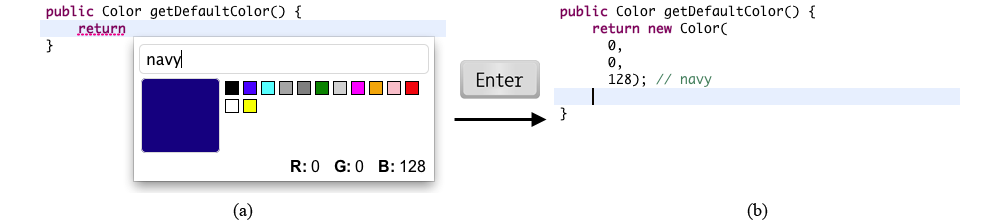
\includegraphics[width=40pc]{color_palette.png}\end{center}
\caption{(a) An example code completion palette associated with the \texttt{Color} class. (b) The source code generated by this palette.}
\end{figure*}

% %\section{Work To Be Done}
\subsection{Completion and Evaluation of Ace}
The work done so far on the Ace language establishes the practicality of active typechecking and translation as a foundational language mechanism and begins to apply it to one realistic problem domain, high-performance scientific computing on GPUs and other coprocessors, by internalizing OpenCL. However, to more fully establish the practicality of this approach, it must be shown that Ace can support more sophisticated, higher-level language constructs as well, ideally from a variety of application domains. It must also be further shown that users who are not language design experts, and will not be utilizing the extension mechanism directly, can nevertheless use the language in practice. 

Thus, a portion of the resources allocated to this project will be dedicated to completing the implementation of Ace, documenting it and releasing it both to the research community and to practitioners in areas where a useful set of constructs have been developed, beginning with the members of the high-performance computing community. This will also support synergy with ongoing collaborations in our group with other problem domains, including front-end and back-end web development, security, functional programming and object-oriented programming.

With broader usage by the research community and in practice, we will be able to continue to conduct case studies and empirical evaluations examining the usability and usefulness of Ace and the active typing mechanisms it introduces. Indeed, because of the flexibility of active typing and our implementation strategy, we plan on instrumenting the Ace compiler to send data and direct feedback from willing users back to us for analysis. This will allow us to analyze questions like:
\begin{itemize}
\item How often are different constructs and mechanisms used in practice?
\item What kinds of errors appear most frequently in practice, and how long does it take users to resolve these errors?
\item How do users feel about the mechanisms, constructs and error messages that they encounter, as determined by direct feedback solicited at the time of occurrence.
\item How commonly do users utilize the active typing mechanism directly?
\end{itemize}

To our knowledge, no such detailed study of usage patterns of a programming language in the wild has been conducted previously, and we anticipate producing insights that are relevant to programming language design broadly.
\subsection{Active Type Theory}
The work on Ace is aimed at establishing a practical implementation of active typechecking and translation. However, because it uses a dynamically-typed language, Python, for the type-level language, it is not suitable for rigorous theoretical analysis, nor does it achieve safety in the strictest sense, due to high levels of dynamism exploitable in Python's object model. Moreover, it is a full language and so it does not necessarily distill the essential concepts that we wish to introduce to the research community in their simplest possible form or connect them to existing concepts in the theory of typed programming languages. For these reasons, we plan to develop a minimal type theoretic formulation, which we call $\lambda_{\text{A}}$.

\subsubsection{Type-Level Computation}

We have chosen to use the term \emph{type-level language}, rather than \emph{metalanguage} or, as it is called in the original work on active libraries, \emph{metacode} intentionally. This is because the concept of a type-level language is already well-established and includes a key feature necessary for active types -- the reification of types as compile-time entities that can be manipulated programmatically. We believe that this connection between type-level computation and active types will provide new insights into each mechanism individually, and provide a clean theoretical basis for active typechecking and translation as an extension to type-level computation.

\subsubsection{Active Types and Wadler's Expression Problem}
Another key insight is that in monolithic programming languages, the fixed set of base types can be written as an algebraic datatype. Indeed, in functional implementations of typecheckers, this is precisely what is done, for example for G\"{o}del's \textbf{T}:

\begin{verbatim}
    datatype Type = Arrow of Type * Type 
                  | Nat
\end{verbatim}

If we wish to allow users to introduce new base types and type families, it can then be seen that we face a variant of the expression problem, so named by Wadler \cite{wadler1998expression}. That is, we wish to add new constructors of kind \verb|Type|, but this conventional formulation of datatypes does not allow us to do so. There are competing approaches that aim to solve this problem. The most common is to use object-oriented inheritance, where subtypes of \verb|Type| represent new type families. This is the approach taken in Ace. The functional programming approach is to instead use \emph{open data types} \cite{conf/ppdp/LohH06}. We will thus aim to further explore this approach, drawing a clear connection between active types, the expression problem and type-level open data types.

\subsubsection{Rigorous Safety Proofs}
A benefit of a simple core theory for active typing is that it will allow us to formally state and prove key safety theorems, formalizing the somewhat informal notions described in Section 3.3. Based on early sketches of a theory that we have discussed, we have implemented some run-time checks into Ace that ensure some of these properties for compiled programs based on a notion borrowed from the area of verified compilation called \emph{type-directed compilation} \cite{tarditi+:til-OLD}. We would like to be able to ensure these properties for all possible programs, and a type theory will allow us to demonstrate the machinery needed to do this in a rigorous manner.

\subsubsection{Implementation With a Dependently-Typed Language}
Finally, we would like to implement a functional version of active type-checking and translation, both as a counterpoint to Ace and as a useful tool for theoretical researchers. We plan on doing so as an extension to the Coq theorem prover, which contains a dependently-typed functional programming language at its core, and is implemented in Ocaml. This will allow us to understand the challenges and opportunities of using a dependently-typed functional language at the core of an extensible programming system.
 
\subsection{Active Code Prediction}
\subsubsection{Structured, Statistical Code Prediction}

Programming languages are formal systems with rich syntactic and semantic structure. They are
also human systems, in that they are used extensively by people in patterned ways to express their
intent. Many tools are designed to help people write code more efficiently by predicting
the source code that a developer intends. For example, code completion systems for editors like Eclipse for Java display pop-up menus containing the members of the class of the variable being manipulated by the developer.

Typical code completion systems use only this sort of semantic
information about the language and the libraries being used, and do not incorporate data about how developers have written programs
in the past. Recent work by Hindle et al.~\cite{Hindle:2012:NS:2337223.2337322} demonstrated, however, that source code could be successfully predicted statistically
using a simple $n$-gram model that used a tokenized, rather than structural, representation of source code, trained on existing codebases.

Our first aim is to unite the structured and statistical approaches to source code prediction. That is, rather than using a tokenized representation of source code, we would like to do statistical prediction on a more natural representation of source code: the typed syntax tree.  We can then condition our predictions using semantic information, specifically:
\begin{itemize}
\item the \emph{type}, denoted $\tau$, of the expression being predicted (e.g. \verb|int| or \verb|Color|)
\item the \emph{syntactic context}, denoted $\sigma$, in which the expression occurs (e.g. whether the expression is an argument of a function call, the guard of an \verb|if| statement, etc.)
\item the \emph{program context}, denoted $\Gamma$, in which the expression occurs (i.e. the set of variables paired with their types that are in scope at the location that the expression occurs.)
\end{itemize}

For example, if a user has entered the code \texttt{Planet destination = }, where \verb|Planet| is an enumeration containing \verb|Mercury|, \verb|Venus|, \verb|Earth|, etc. (but not \verb|Pluto|, of course), then we have that the expected type at the cursor is \verb|Planet|, the syntactic context is \emph{assignment}, and given a program context, our prediction space should only assign non-zero probabilities to:
\begin{itemize}
\item literal members of the \verb|Planet| enumeration (e.g. \verb|Planet.EARTH|)
\item variables and fields of type \verb|Planet| available from the program context
\item calls to methods available from the program context that have return type \texttt{Planet}\footnote{We can consider  operators like $+$ and $[]$ as methods of the built-in types in Java.}
\end{itemize}
To assign a particular probability to an expression, denoted $e$, we first determine how likely it is that the expression is of each of these three \emph{syntactic forms}, where syntactic forms are denoted $\phi$. For each form, we can then assign probabilities to particular expressions of that form according to some form-specific conditional distribution. This model can be understood as a graphical model, as shown in Figure \ref{graphicalmodel}, where the syntactic form is a latent variable. The conditional distributions for both the syntactic form and expression are learned using data gathered from analyses of prior code corpuses (smoothed using a suitable method in cases where enough information is not available).
\begin{figure}
    \begin{displaymath}
    \xymatrix{
      *+[F]{\color{ForestGreen}\txt{Type ($\tau$)}} \ar[dr] \ar[drr] & & \\
      & *+[F]{\color{black} \txt{Syntactic\\Form ($\phi$)}} \ar[r] & *+[F]{\color{cyan}\txt{Expression ($e$)}}  \\
      *+[F]{\color{ForestGreen}\txt{Syntactic\\Context ($\sigma$)}} \ar[ur] \ar[urr] & & *+[F]{\color{ForestGreen}\txt{Program\\Context ($\Gamma$)}} \ar[u]  
    }
    \end{displaymath}
\caption{\small A graphical model representing our approach. Green variables are always observed (we do not assign marginal distributions to them.) The syntactic form, $\phi$, is a latent variable, and the expression, $e$, is unknown. Note that the syntactic form is a function of the expression. \label{graphicalmodel}}
\end{figure}

\subsubsection{Active Code Prediction}
Given a system for predicting expressions in the context of a type syntax tree, we can then naturally ask: what about specialized domain knowledge that cannot be readily extracted from prior code analysis? For example, consider a type representing strings in a particular language, such as English. Constructors of the \verb|EnglishString| type should be biased to accept literals that have high likelihoods according to some natural language model, but we do not wish to encode all possible natural language models in the core of our prediction system. We can instead take an active types approach by allowing users to equip a type, such as \verb|EnglishString|, with a function, $f_{\text{prob}}$, that takes on the job of predicting the probabilities of only expressions of that type. That is, given a reified representation of $\sigma$, $\Gamma$ and $\phi$, it should be able to produce $P(e | \tau, \phi, \sigma, \Gamma)$. We can then use this prediction directly as if it had been produced by a method described above.

\subsubsection{Foundations, Implementation and Analysis}
We propose developing the theoretical foundations of this idea, in terms of probability theory and type theory, equipping it with a notion of active code prediction as described above, and implementing this atop a real language, likely Java. We have sketched and prototyped a small version of this as an Eclipse extension in the context of a prior course project. We will then evaluate the accuracy of these models, develop use cases as in the related work on active code completion described in Section \ref{graphite}, and analyze the usability and usefulness of this prediction system in applied contexts. In particular, we are interested in uses within code editors to predict expressions and portions of expressions, as well as uses within programming systems for disabled and paralyzed individuals, who need predictive text entry to be able to communicate at a reasonable pace. The information theoretic foundations for this latter application, in the context of brain-computer interfaces, have been developed as prior work by one of the investigators on this proposal \cite{journals/ijhci/OmarAJBMMMC11}.

%\subsection{Syntax and Visual Representation}
%Thus far, we have been discussing active types within the context of languages with a fixed syntax. However, in many specialized domains, a specialized syntax or visual representation for novel constructs may be appropriate. There are several approaches that we can take to include extensible syntax support in an actively-typed programming system. We have not settled on any one of these, so our proposed research will include a rigorous examination of the pros and cons of each approach.
%
%\subsubsection{Extensible Parsing} 
%Extensible parsers have been well-studied in the literature (e.g. \cite{journals/entcs/BrabrandSV03}), and such systems could be integrated with an actively-typed language without conflict with one caveat: each new syntactic form needs to have a dispatch protocol associated with it, to assign control over its semantics to one of its subexpressions. Such a mechanism will be one avenue we will evaluate for suitability.
%
%\subsubsection{Flexible Reinterpretation}
%An approach that we have prototyped, but not extensively utilized, in Ace is to allow active types to directly observe the syntax trees of subexpressions, rather than simply their types as we have described above. This allows a highly contextualized reinterpretation of a syntax tree, similar to capabilities found in macro systems (although without a direct rewriting component.) We will further explore this approach, particularly as we begin implementing abstractions that may not naturally fit within Python's existing syntactic forms in an intuitive way.
%
%\subsubsection{Delimited Parsing}
%A related alternative approach would be to partially parse a file, leaving delimited regions either unparsed or only tokenized and dispatching to an active type to do the actual parsing. This would give more flexibility to the active type, but also a greater responsibility to fully parse and give semantics to the provided source code. Nevertheless, this may be appropriate in certain cases where a highly-specialized local syntax is desirable for convenience (and flexible reinterpretation or active code completion at edit-time does not suffice.)
%
%\subsubsection{Actively-Typed Structured Editors}
%Projects such as Citrus \cite{Ko05} and Barista \cite{Ko06} are analogs of language frameworks for structured editors -- editors where source code elements are represented directly as a tree in a visual or semi-visual form, rather than written as a string as in conventional languages. These tools demonstrate that modular construction of such editors may be possible. An actively-typed structured editor would instead allow an active type to directly control the visual representation and interaction behaviors associated with expressions of that type. This is the most direct analog of active types in this domain, but requires a somewhat radical shift in program representation. It is unlikely that this can be integrated easily into existing languages and systems, as we have largely done in our other work. Thus, we will develop a separate prototype of this approach, and believe that the long-term evolution of actively-typed programming systems will be toward such a representation.

% % !TEX root = omar-thesis-proposal.tex
\section{Timeline}

\subsection{Fall 2013}
I will complete the work on Ace (ESOP - Oct.) and active type theory (PLDI - Nov.) and Wyvern (ECOOP - Dec.) and submit each for publication.

Ace:
- Finish implementation
- Finish OpenCL implementation
- Finish C implementation
- Implement global arrays, functional data parallelism, objects

Theory:
- Prove metatheory (mechanized?)
- Figure out composition theorem
- Figure out how it would look in Coq

Wyvern:
- Figure out grammar and type system formalism
- See implementation through
- Declarative stuff
- Write it up

Graphite:
- Figure out safety stuff

\subsection{Spring 2014}
I will finalize all work and write the final dissertation.

%\subsection{Summer 2014}

% !TEX root = globaldsl13.tex
%\section{Conclusion} % and Future Work}
%\label{s:conclusion}
%
%In this paper, we described how extensible parsing in Wyvern makes for
%a solid platform to support whitespace-delimited, type-directed embedded DSLs. In the
%future, we aim to implement a wide variety of DSLs in Wyvern tweaking
%our approach and implementation thereof to provide a comprehensive example of
%supporting multiple interacting DSLs in a safe and easy-to-use manner.
%
% \todo{tie features to goals}

% \todo{implementation and validation plans}

\section*{Acknowledgements}
We thank the anonymous reviewers for helpful comments, and acknowledge the support of the Department of Defense and the Air Force Research Laboratory. CO is supported by the NSF Graduate Research Fellowship.

\newpage

%% Bibliography magic
% dvips -n 15 -o description.ps description
% dvips -p=16 -o bibliography.ps description
% ps2pdf description.ps
% ps2pdf bibliography.ps
%
% OR, for pdflatex:
%
% pdftk description.pdf cat 1-15 output description1.pdf
% pdftk description.pdf cat 16-end output bibliography.pdf

\setcounter{page}{1}
\renewcommand{\thepage}{References - \arabic{page}}

\bibliographystyle{abbrv}
\bibliography{../research}
%,typestate-verification,objects,ownership,formal,dynamicweb,cloud
%\bibliographystyle{plainnat}
%\bibliography{references,dynamicweb,cloud}

\end{document}
